%% `numberedappendix` AND `appendixfloats` are both required, not cosmetic.
%% Without `numberedappendix` the class sets
%% `\AppendixApjSectionMarkInTitle#1{\relax}`, so an appendix heading prints
%% its title and NO LETTER -- while the body cites "Appendix~D.2" and
%% "\S D.2", and the reader is then sent to a label that is nowhere on the
%% page.  The letters and the subsection numbers are in
%% `\thesection`/`\thesubsection` either way and are simply not typeset
%% without it.  `appendixfloats` makes the appendix floats carry their
%% appendix's letter (A1, B1, D1, D2, E1) and restart at one in each;
%% without it an appendix figure cited seventh from the main text prints as
%% "Figure 10" and the main-text sequence looks wrong when it is not.
%% Every reference is a \ref, so nothing in the prose is typed.
\documentclass[twocolumn,twocolappendix,numberedappendix,appendixfloats]{openjournal}

%% ★★★ v4.25: PIN THE TRAILER /ID.  pdfTeX derives the PDF's trailer /ID from
%% an MD5 of the OUTPUT FILENAME and the build timestamp, so the same source
%% built as a different .tex name produced a PDF differing in exactly those 32
%% hex digits and in nothing else.  That made two things we need mutually
%% exclusive: `arxivset.sh`'s A8 proof that the stripped package is
%% byte-identical to the in-tree build, and a submission package whose
%% top-level filename carries no internal version string.  With the ID pinned
%% the PDF is a function of the source alone -- SOURCE_DATE_EPOCH already pins
%% the timestamp half of the same hash.  Guarded, because \pdftrailerid is a
%% pdfTeX primitive and the paper must still compile under an engine without
%% it (the ID is then filename-derived again, which is the old behaviour).
\ifdefined\pdftrailerid
  \pdftrailerid{alma-narrowband-carrier-search-40pc}
\fi

%% ★★★★ v4.25: AND THE PDF ITSELF CARRIED A VERSION STRING, WHERE NO TEXT
%% SWEEP COULD SEE IT.  For every included PDF figure pdfTeX writes the path
%% it was included from into the XObject dictionary as `/PTEX.FileName`, so
%% the shipped file held eleven local paths -- among them
%% `./figures/chain_v412.pdf`, the one occurrence of `_v4` anywhere in the
%% binary.  `pdftotext` cannot see it (it is a dictionary entry, not a text
%% stream), so `genai_sweep`, `prose_v412` and the forbidden-mention sweep all
%% passed a PDF that named an internal revision.  Suppressing the three PTEX
%% entries removes it, removes ten other local build paths with it, and makes
%% the output independent of where the figures sit -- which is also what lets
%% `arxivset.sh`'s A15 rename them in the package and A8 still prove the
%% clean build byte-identical.
\ifdefined\pdfsuppressptexinfo
  \pdfsuppressptexinfo=-1
\fi

%% ★★★★ AND THE DEFECT THE OPTION ABOVE CREATED, FOUND BY `labelcheck` F7 AND
%% NOT BY pdflatex.  `appendixfloats` resets the float counters in each
%% appendix, so the PRINTED numbers are right -- A1, C1, D1, D2 -- while the
%% HYPERREF ANCHOR is built from the bare counter and is `table.1` for all
%% four of the appendix tables at once.  Every body hyperlink to Table D1 then
%% lands on Table 1, which is the fifth defect of this project that the log
%% cannot see and a reader can.  `\theH...` is hyperref's own hook for exactly
%% this: it must carry whatever makes the number unique, which here is the
%% appendix letter.
\makeatletter
\AtBeginDocument{%
  \renewcommand{\theHtable}{\thesection.\arabic{table}}%
  \renewcommand{\theHfigure}{\thesection.\arabic{figure}}%
  \renewcommand{\theHequation}{\thesection.\arabic{equation}}%
}
\makeatother

\usepackage[T1]{fontenc}
\usepackage{graphicx}
\usepackage{amsmath,amssymb}
\usepackage{hyperref}
\usepackage{array}

\newcolumntype{P}[1]{>{\raggedright\arraybackslash}p{#1}}
\usepackage{booktabs}
%% The crossing ledger is fifteen columns wide and is set landscape, which
%% is what lets every one of its rows print at the same size as the rest of
%% the tables in this paper rather than two points below the body text.
\usepackage{rotating}
%% ★★★★ AND THE SIDEWAYS FLOAT HAS TO BE PUT BACK ON THE PAGE.  `rotating`
%% places a rotated double float with `\@@line`, which is `\hbox to \hsize`,
%% and sets `\hsize\textwidth` itself when it opens the float -- but this
%% class is derived from revtex4, whose own float machinery leaves \hsize at
%% the COLUMN width by the time the box is placed.  The rotated box was
%% therefore centred on column one instead of on the page: measured on the
%% shipped v4.19 build, the crossing ledger's caption ran from x = -5.9 pt,
%% i.e. off the left edge of the paper, with the first word or two missing
%% from every line of a nineteen-line caption, and 133 pt of the page's width
%% stood empty on the right.  No gate saw it: rotation hides the overflow
%% from `Overfull \hbox`, and nothing in this build had ever measured ink
%% against the text block.  `rotfit_r18.py` measures it now.
%% The patch restores the width the package meant to use, at the one point
%% where it is read.  `\patchcmd` fails loudly rather than silently doing
%% nothing, because a patch that stops applying after a package update would
%% put the caption back off the page.
\usepackage{etoolbox}
\makeatletter
\patchcmd{\end@rotdblfloat}{\vbox to \textheight}%
  {\hsize\textwidth\linewidth\textwidth\vbox to \textheight}%
  {}{\ClassError{technosignatures}{rotating's \string\end@rotdblfloat\space
      could not be patched: the sideways ledger would print off the page}{}}
\makeatother

%% ★★★ v4.11: SUPPRESS THE CLASS'S PREPRINT VERSION STAMP (referee 2, first
%% minor).  `openjournal.cls` sets `\submitted{Version \today}` and then
%% `\journalinfo{\@submitted}`, so the line is typeset twice -- once as the
%% title-page slug and once in the journal-info header -- and it was the
%% first thing on page 1.  The build pins SOURCE_DATE_EPOCH so that the
%% figures and the PDF are byte-identical run to run, which means `\today`
%% reads "January 1, 2020" and would read that for ever.
%%
%% The date is therefore NOT unfrozen: a reproducible build is worth more
%% than a date, and a date that must never change should not be printed at
%% all.  A journal submission does not want a preprint version stamp
%% either.  Both are emptied here rather than in the class, which is a
%% third-party template the journal may replace.  `abswords.py` and the
%% LaTeX-log gate both read page 1, so a regression shows up there.
\submitted{}
\journalinfo{}
% suppress the class's end-of-document template advertisement;
% delete this block to restore it
\makeatletter
\renewenvironment{bottompar}{\setbox\z@\vbox\bgroup}{\egroup}
%% ★ v4.16: AND THE SAME ADVERTISEMENT AT THE TOP OF PAGE 1, which the
%% end-of-document suppression above did not reach.  "Preprint typeset using
%% LaTeX style openjournal v. 09/06/15" was the first line of the paper --
%% above the title -- and it is a property of the template, not of the work.
%% Referee 2's first minor point was about exactly this kind of slug printed
%% where a reader looks first; \submitted and \journalinfo were emptied for it
%% and this line was left.  The \vspace that follows it is kept, so the title
%% block does not move and no page count changes.
\long\def\frontmatter@title@above{%
  \vspace*{-\headsep}\vspace*{\headheight}%
  \footnotesize
  {\footnotesize\textsc{\@journalinfo}}\par
  \par\vspace*{-\baselineskip}\vspace*{0.625in}%
}%
\makeatother

% ---------------------------------------------------------------
% \pv{\Macro} -- print a probability with its relational symbol.
% Generated p-value macros are of two kinds: an ordinary value such as
% 0.186, and a bound such as <10^{-4} for a probability too small for the
% ensemble to resolve. Writing "$p=\Macro$" at the use site is right for
% the first and produces "p =< 10^-4" for the second; writing "$p\Macro$"
% is right for the second and produces "p0.186" for the first. Both
% mistakes were in the manuscript. The relation therefore belongs with
% the value, decided once, here: \pv inspects the first token of the
% expanded macro and supplies "=" unless the value already carries its
% own relational symbol.
\makeatletter
\def\@pvlt{<}\def\@pvgt{>}\def\@pveq{=}
\def\@pvfirst#1#2\@nil{%
  \def\@pvA{#1}%
  \ifx\@pvA\@pvlt <#2%
  \else\ifx\@pvA\@pvgt >#2%
  \else\ifx\@pvA\@pveq =#2%
  \else =#1#2\fi\fi\fi}
\DeclareRobustCommand{\pv}[1]{p\,\expandafter\@pvfirst#1\@nil}
\makeatother
% ---------------------------------------------------------------
% \rankstatus -- the status of the star-versus-control rank, in ONE
% formulation used verbatim wherever the question arises (referee 1, item 1).
% Earlier versions stated this in several incompatible ways: the main text
% denied exchangeability while Appendix A asserted that star and controls
% "remain exchangeable in signal-to-noise ratio", and a table caption called
% the ensemble a "calibrated screen".  A macro makes the use sites identical
% by construction rather than by proof-reading.
\DeclareRobustCommand{\rankstatus}{The star-versus-control rank is an
empirically useful way of deciding which crossing to examine first, but the
stellar and control positions are not demonstrably exchangeable under the
null. The rank therefore has no calibrated per-window false-alarm probability
and is not used as evidence for detection.}
% ---------------------------------------------------------------
\shorttitle{An ALMA Archival Technosignature Search within 40\,pc}
\shortauthors{White \& Dey}

% GENERATED by make_numbers.py -- do not edit by hand.
% Every survey quantity in the manuscript is defined here, once,
% from survey_stats.json / occurrence_v328.json / nullcal.json.
\newcommand{\NCensus}{168}
\newcommand{\NStars}{90}
\newcommand{\NSystems}{83}
\newcommand{\NStarBands}{113}
\newcommand{\NEB}{407}
\newcommand{\NExtracted}{1721}
\newcommand{\NDup}{45}
\newcommand{\NDefect}{13}
\newcommand{\NWithheld}{0}
\newcommand{\NWindows}{1663}
\newcommand{\NFine}{405}
\newcommand{\NCoarse}{1258}
\newcommand{\DistMin}{1.30}
\newcommand{\DistMax}{39.63}
\newcommand{\UnionGHz}{118.1}
\newcommand{\UnionIntervals}{46}
\newcommand{\UnionLo}{89.6}
\newcommand{\UnionHi}{873.1}
\newcommand{\ExposureSGHz}{6.9\times10^{6}}
\newcommand{\EirpMin}{1.6\times10^{13}}
\newcommand{\EirpMax}{2.8\times10^{17}}
\newcommand{\EirpMedian}{7.0\times10^{14}}
\newcommand{\SminMin}{0.41}
\newcommand{\SminMax}{1.31}
\newcommand{\SminMedian}{9.9}
\newcommand{\ChanMedianMHz}{15.625}
\newcommand{\NHits}{56}
\newcommand{\NSpatial}{12}
\newcommand{\NSpatialOld}{18}
\newcommand{\NLineAttrib}{10}
\newcommand{\NUnattrib}{2}
\newcommand{\NCandidates}{0}
\newcommand{\NCtrl}{512}
\newcommand{\RankFloor}{513}
\newcommand{\ExpFlags}{3.24}
\newcommand{\NRankFirst}{14}
\newcommand{\RateRankFirst}{0.8}
\newcommand{\RateRankFirstOld}{8.9}
\newcommand{\NRankFirstOld}{148}
\newcommand{\TrialCells}{1.32\times10^{8}}
\newcommand{\NPseudo}{220\,672}
\newcommand{\PseudoKSp}{0.37}
\newcommand{\PseudoMean}{0.5010}
\newcommand{\StarPseudoP}{0.38}
\newcommand{\OccMeasured}{5.7}
\newcommand{\OccMeasuredRound}{6}
\newcommand{\OccUnit}{3.4}
\newcommand{\OccUniform}{8.1}
\newcommand{\OccDhalf}{7.6}
\newcommand{\OccDtenth}{19}
\newcommand{\NOccSystems}{66}
\newcommand{\NOccSystemsUnit}{87}
\newcommand{\IntGainSpan}{16}
\newcommand{\FineOnsrcMedian}{2177}
\newcommand{\CalibOnsrc}{1506}
\newcommand{\CalibGainRatio}{1.2}
\newcommand{\SbrN}{14}
\newcommand{\SbrPobs}{1.7\times10^{-3}}
\newcommand{\SbrAstro}{3}
\newcommand{\SbrResid}{2}
\newcommand{\SbrResidP}{0.21}
\newcommand{\OnsrcMin}{21}
\newcommand{\OnsrcMax}{5274}
\newcommand{\MasonRatio}{1250}
\newcommand{\OnsrcMedian}{2087}
\newcommand{\DutyHalf}{7.6}
\newcommand{\DutyTenth}{19}
\newcommand{\DutyHalfUnit}{4.5}
\newcommand{\NMultiEpoch}{55}
\newcommand{\AuPct}{92.1}
\newcommand{\AuNge}{34}
\newcommand{\AuFrac}{7.9}
\newcommand{\AuP}{0.081}
\newcommand{\CtrlMed}{4.56}
\newcommand{\CtrlPninety}{5.85}
\newcommand{\NNonBP}{416}
\newcommand{\NBPWindows}{15}
\newcommand{\NDwellTrials}{3\,888}
\newcommand{\NDwellWin}{12}
\newcommand{\DwellCoarseOne}{100}
\newcommand{\DwellCoarseQ}{100}
\newcommand{\DwellCoarseT}{83}
\newcommand{\DwellFineOne}{100}
\newcommand{\DwellFineQ}{91}
\newcommand{\DwellFineT}{71}
\newcommand{\RecThresh}{42}
\newcommand{\RecThreshHi}{16}
\newcommand{\RecThreshLo}{14}
\newcommand{\RecTwice}{83}
\newcommand{\NTrials}{1200}
\newcommand{\PctBandsSixSeven}{91}

% survey_numbers_round8.tex -- generated by round8_calc.py
% from frozen_export_v3.31.json + occurrence_v328.json +
% dwell_campaign_trials_v3.32.csv (v3.31/v3.32 freezes).
% class widths / eta on frozen classes, EB reconciliation, f95
% ICC sensitivity, flag effect sizes, defect localisation,
% dwell-campaign criterion cross-check; referee round 8.

\newcommand{\ChanAMinKHz}{15.259}
\newcommand{\ChanAMaxKHz}{1953.125}
\newcommand{\ChanAMedKHz}{488.3}
\newcommand{\ChanAModeKHz}{488.3}
\newcommand{\ChanAModePct}{60}
\newcommand{\ChanBMinMHz}{7.812}
\newcommand{\ChanBMaxMHz}{31.25}
\newcommand{\ChanBMedMHz}{15.625}
\newcommand{\ChanBModeMHz}{15.625}
\newcommand{\ChanBModeN}{1218}
\newcommand{\ChanGapFac}{4.0}
\newcommand{\ChanStraddleKHz}{1953.125}
\newcommand{\EtaStraddle}{1.46}
\newcommand{\EtaAmin}{0.17}
\newcommand{\EtaAmed}{14.7}
\newcommand{\EtaAmax}{422}
\newcommand{\EtaAltOne}{14}
\newcommand{\EtaBmin}{0.004}
\newcommand{\EtaBmed}{0.51}
\newcommand{\EtaBmax}{1.35}
\newcommand{\EtaBgeOne}{38}
\newcommand{\EtaBgeOneMax}{1.35}
\newcommand{\DgridA}{0.26}
\newcommand{\DgridB}{0.29}
\newcommand{\EbsRetained}{407}
\newcommand{\EbsRankAll}{407}
\newcommand{\EbsExtraN}{0}
\newcommand{\EffEbsFine}{255}
\newcommand{\EffKbar}{1.59}
\newcommand{\EffDeff}{1.14}
\newcommand{\EffSumC}{50.6}
\newcommand{\EffFIccPct}{6.5}
\newcommand{\NFlagWin}{12}
\newcommand{\NFlagSys}{4}
\newcommand{\NFlagBpic}{9}
\newcommand{\NFlagOther}{3}
\newcommand{\DefectNoSib}{1}
\newcommand{\DefectOnsrcLo}{12}
\newcommand{\DefectOnsrcHi}{2842}
\newcommand{\DefectRmsLoSci}{4.5\times10^{-4}}
\newcommand{\DefectRmsHiSci}{14.3\times10^{-4}}
\newcommand{\DefectSibFacLo}{388}
\newcommand{\DefectSibFacHi}{743}
\newcommand{\DefectBandSix}{7}
\newcommand{\DefectBandSeven}{6}
\newcommand{\DefectNStars}{8}
\newcommand{\XcheckN}{3888}
\newcommand{\XcheckAgree}{3888}
\newcommand{\XcheckMismatch}{0}
\newcommand{\XcheckTrueMin}{5.04}
\newcommand{\XcheckFalseMax}{5.00}
\newcommand{\XcheckWin}{12}
% retired by retire_macros.py (unreferenced): BandWinEight, BandWinFive, BandWinFour, BandWinNine, BandWinSeven, BandWinSix, BandWinTen, BandWinThree, MarginBpicSix, MarginBpicThree, MarginCp, MarginHd, ZetaBpicSix, ZetaBpicThree, ZetaCp, ZetaHd

% survey_numbers_round9.tex -- generated by round9_calc.py
% from frozen_export_v3.31.json; mask-union framing derived
% from the generated Table tab:maskband (4.96 GHz all-species
% merged Union); referee round 9 (R4-B concentration, R3-8
% mask framing, R3-3 CP-72 2713 feature rows).

\newcommand{\ConcThreeNames}{BD$+$05~1668, Proxima Cen and HD~33793}
\newcommand{\ConcThreeWin}{285}
\newcommand{\ConcThreePct}{17.1}
\newcommand{\ConcThreeSys}{3}
\newcommand{\CpTwoFreqGHz}{345.1152}
\newcommand{\CpTwoTstar}{5.81}
\newcommand{\CpTwoRingMax}{5.68}
\newcommand{\CpTwoMargin}{0.13}
\newcommand{\CpTwoLineOffKms}{-1326}
\newcommand{\CpTwoNdrift}{129}
\newcommand{\CpTwoDriftkHzs}{4.14}
\newcommand{\CpTwoBwGHz}{1.73}
\newcommand{\CpTwoOnsrcS}{2994}

%% GENERATED by round10_calc.py -- do not hand-edit.
\newcommand{\CompWin}{12}
\newcommand{\CompTgt}{11}
\newcommand{\CompBands}{3, 6 and~7}
\newcommand{\CompNintLo}{21}
\newcommand{\CompNintHi}{1\,314}
\newcommand{\CompNintFactor}{63}
\newcommand{\CompFiftyN}{6}
\newcommand{\CompFiftyLo}{5.3}
\newcommand{\CompFiftyHi}{8.3}
\newcommand{\CompFiftyMed}{6.2}
\newcommand{\CompSatN}{6}
\newcommand{\CompSatMin}{3.4}
\newcommand{\CompSatRec}{97}
\newcommand{\OccAll}{4.0}
\newcommand{\NOccAll}{88}
\newcommand{\OccAllDhalf}{5.4}
\newcommand{\OccAllDtenth}{13}
\newcommand{\OccAllFifteen}{8.6}
\newcommand{\NOccAllFifteen}{76}
\newcommand{\OccAllSeventeen}{3.5}
\newcommand{\NOccAllSeventeen}{88}

%% GENERATED by round10_calc.py (v3.41 block) -- do not hand-edit.
\newcommand{\GrossBwGHz}{2849.5}
\newcommand{\GaussCross}{37.9}
\newcommand{\PgeFourPct}{40.7}
\newcommand{\ExpNonBP}{3.14}
\newcommand{\PgeOneNonBPPct}{96}
\newcommand{\FlagPairs}{5}
\newcommand{\FluxBpicThree}{76}
\newcommand{\FluxBpicSix}{78}
\newcommand{\FluxHdFour}{0.82}
\newcommand{\FluxCpSeven}{12}
\newcommand{\FluxRatioBpic}{1.0}
\newcommand{\MaskRestRoundMHz}{1}
\newcommand{\CatCOoneGHz}{115.271000}
\newcommand{\LabCOoneGHz}{115.271202}
\newcommand{\CatCOerrMHz}{0.202}
\newcommand{\CatCOerrKms}{0.53}
\newcommand{\CatWorstKms}{1.3}
\newcommand{\VsysBpic}{+20.0}
\newcommand{\VsysBpicErr}{0.7}
\newcommand{\DnuBpicCoarse}{-9.62}
\newcommand{\DvBpicCoarse}{-12.51}
\newcommand{\StelBpicThree}{-0.39}
\newcommand{\StelBpicSix}{-0.29}
\newcommand{\StelBpicCoarse}{-0.14}
\newcommand{\BpicSpreadKms}{0.2}
\newcommand{\BpicPairSepKms}{0.09}
\newcommand{\BpicMaxAbsStel}{0.39}
\newcommand{\BpicMaskPct}{0.8}
% retired by retire_macros.py (unreferenced): BaryBpicCoarse, BaryBpicSix, BaryBpicThree, DnuBpicSix, DnuBpicThree, DnuCpSeven, DnuHdFour, DvBpicSix, DvBpicThree, DvCpSeven, DvHdFour, FcenBpicSix, FcenBpicThree, FcenCpSeven, FcenHdFour, FobsBpicSix, FobsBpicThree, FobsCpSeven, FobsHdFour

%% GENERATED by v342_calc.py -- do not hand-edit.
\newcommand{\RingSeed}{20260825}
\newcommand{\RingNProbe}{512}
\newcommand{\RingNSrc}{135}
\newcommand{\RingInFrac}{0.14}
\newcommand{\RingOutFrac}{0.78}
\newcommand{\RingCheckFrac}{0.06}
\newcommand{\RingGainIn}{0.95}
\newcommand{\RingGainOut}{0.19}
\newcommand{\RingGainMean}{0.47}
\newcommand{\RingGainInTrue}{0.98}
\newcommand{\RingGainOutTrue}{0.51}
\newcommand{\RingPbCoef}{1.13}
\newcommand{\RingPbCoefCode}{1.22}
\newcommand{\RingThetaMin}{7.2}
\newcommand{\RingThetaMax}{69.5}
\newcommand{\RingRinMin}{1.0}
\newcommand{\RingRinMax}{9.7}
\newcommand{\RingRoutMin}{5.6}
\newcommand{\RingRoutMax}{54.2}
\newcommand{\RingRhoCO}{0.05}
\newcommand{\RingRhoCOexp}{-1}
\newcommand{\RingRhoNull}{0.002}
\newcommand{\RingRhoNullN}{1195}
\newcommand{\RingRhoNullLo}{-0.10}
\newcommand{\RingRhoNullHi}{0.10}
\newcommand{\RingRhoBoundPct}{10}
\newcommand{\HdThirteenOffset}{15.9}
\newcommand{\HdThirteenOffsetPB}{0.55}
\newcommand{\HdThirteenTopLo}{11.4}
\newcommand{\HdThirteenTopHi}{22.2}
\newcommand{\HdThirteenRingMed}{15.9}
\newcommand{\HdThirteenRingMax}{10.8}
\newcommand{\HdThirteenStar}{4.4}
\newcommand{\MaskNTransOld}{15}
\newcommand{\MaskNTransNew}{17}
\newcommand{\MaskNSpecOld}{9}
\newcommand{\MaskNSpecNew}{11}
\newcommand{\MaskCIGHz}{492.160651}
\newcommand{\MaskHthirtyGHz}{231.900928}
\newcommand{\MaskVWidth}{50}
\newcommand{\MaskRoundWorstKms}{1.59}
\newcommand{\PeakFreqMatched}{287}
\newcommand{\MaskFrameChained}{4}
\newcommand{\MaskFrameTotal}{12}
\newcommand{\MaskNewCoinc}{0}
\newcommand{\MaskLostOldGHz}{0.64}
\newcommand{\MaskLostNewGHz}{0.88}
\newcommand{\MaskExtraGHz}{0.24}
\newcommand{\MaskExtraPct}{0.2}
\newcommand{\NCrossFreq}{51}
\newcommand{\HanBest}{0.50}
\newcommand{\HanWorst}{0.42}
\newcommand{\HanMed}{0.48}
\newcommand{\HanFacBest}{2.00}
\newcommand{\HanFacWorst}{2.36}
\newcommand{\HanFacMed}{2.08}
\newcommand{\HanFacAvgLo}{1.18}
\newcommand{\HanFacAvgHi}{1.96}
\newcommand{\HanFacAvgMed}{1.33}
\newcommand{\NNoArchResBands}{none}
\newcommand{\NNoArchRes}{0}
\newcommand{\HanArchHi}{2.000}
\newcommand{\HanArchLo}{1.156}
\newcommand{\HanArchNHi}{1516}
\newcommand{\HanArchNLo}{146}
\newcommand{\HanNByN}{$n=1$: 1516, $n=2$: 146, $n=4$: 1}
\newcommand{\HanNFour}{1}
\newcommand{\HanFwhmFour}{1.0143}
\newcommand{\HanFacFourMed}{1.06}
\newcommand{\HanFacFourLo}{0.98}
\newcommand{\HanFacFourHi}{1.90}
\newcommand{\EirpMinA}{2.2\times10^{13}}
\newcommand{\EirpMaxA}{6.9\times10^{16}}
\newcommand{\ChanLoA}{15.3}
\newcommand{\ChanHiA}{1953}
\newcommand{\NWinA}{405}
\newcommand{\EirpMinB}{1.6\times10^{13}}
\newcommand{\EirpMaxB}{2.8\times10^{17}}
\newcommand{\ChanLoB}{7.812}
\newcommand{\ChanHiB}{31.25}
\newcommand{\NWinB}{1258}
\newcommand{\PctCoarse}{76}
\newcommand{\AsymExpectPct}{20.9}
\newcommand{\PctFine}{24}
\newcommand{\EtaAltOneNow}{14}
\newcommand{\EtaBgeOneNow}{38}
\newcommand{\AmaxMin}{3.6}
\newcommand{\AmaxMax}{4.0}
\newcommand{\CaseDetCoarseNow}{1}
\newcommand{\CaseDetCoarseTwoNow}{4}
\newcommand{\CaseDetFineNow}{11}
\newcommand{\CaseDetDwellNow}{29}
\newcommand{\NSysInTwentyNow}{42}
\newcommand{\NStarBelowAreciboNow}{1}
\newcommand{\NEffArecibo}{0}
\newcommand{\NEffTwiceArecibo}{1}
\newcommand{\DeepestEffSci}{3.4\times10^{13}}
\newcommand{\TuNCatCov}{1649}
\newcommand{\TuNCatUncov}{14}
\newcommand{\TuNCatDupExtract}{67}
\newcommand{\TuNCatAmbig}{2}
\newcommand{\DispoNAttrComputed}{16}
\newcommand{\DispoNAttrRanked}{10}
\newcommand{\DispoNAttrBlank}{6}
\newcommand{\DispoNHandEntries}{12}
\newcommand{\DispoNHandOldEntries}{5}
\newcommand{\DispoNShipped}{12}
\newcommand{\DispoOldKeyReach}{4}
\newcommand{\DispoNMislabel}{2}
\newcommand{\DispoMislabelMinKms}{3794}
\newcommand{\DispoMislabelMaxKms}{3898}
\newcommand{\DispoHalfKms}{50}
\newcommand{\NStarsReleased}{90}
\newcommand{\NCatRows}{1663}
\newcommand{\NCatCols}{62}
\newcommand{\NCatFlagGlobal}{12}
\newcommand{\NCatFlagLocal}{11}
% retired by retire_macros.py (unreferenced): ChanMedA, ChanMedB, EirpHanMaxA, EirpHanMaxB, EirpHanMedA, EirpHanMedB, EirpHanMinA, EirpHanMinB, EirpMedA, EirpMedB

% Generated by v343_calc.py -- do not edit by hand.
\newcommand{\NSmearNoValue}{1208}
\newcommand{\NSmearLo}{9}
\newcommand{\NSmearWorst}{5}
\newcommand{\SmearWorstPenLo}{1.65}
\newcommand{\SmearWorstPenHi}{1.74}
\newcommand{\SmearWorstChanKHz}{15.3}
\newcommand{\NSmearFlagged}{2}
\newcommand{\NSmearOk}{446}
\newcommand{\SmearList}{HIP~10679 Band~6 (0.574, $\times$1.74), $\beta$~Pic Band~6 (0.574, $\times$1.74), HD~172555 Band~6 (0.574, $\times$1.74), HIP~10679 Band~6 (0.606, $\times$1.65), HD~172555 Band~6 (0.606, $\times$1.65), $\eta$~Crv Band~8 (0.865, $\times$1.16), $\eta$~Crv Band~7 (0.932, $\times$1.07), HD~48370 Band~6 (0.979, $\times$1.02) and CP$-$72~2713 Band~6 (0.979, $\times$1.02)}
\newcommand{\PbMedian}{1.00002}
\newcommand{\PbPninety}{1.002}
\newcommand{\NPbAboveTwoPct}{91}
\newcommand{\NPbAboveTenPct}{42}
\newcommand{\PbMaxStar}{eps~Eri}
\newcommand{\PbMaxBand}{6}
\newcommand{\PbMax}{3.52}
\newcommand{\PbMaxRoverTheta}{0.67}
\newcommand{\PbMaxRoverFwhm}{0.73}
\newcommand{\NSirWin}{12}
\newcommand{\PbSirLoPct}{3.6}
\newcommand{\PbSirHiPct}{18.6}
\newcommand{\PbSirRoverThetaLo}{0.11}
\newcommand{\PbSirRoverThetaHi}{0.25}
\newcommand{\NPbTierStars}{6}
\newcommand{\CtrlMaxSurveyMax}{19.7}
\newcommand{\CtrlMaxSurveySecond}{19.5}
\newcommand{\BpicNFlagThree}{5}
\newcommand{\BpicNFlagSix}{4}
\newcommand{\BpicBThreeTsym}{30.76}
\newcommand{\BpicBSixTsym}{11.68}
\newcommand{\BpicAddOneDen}{1664}
\newcommand{\BpicCoRingMax}{18.3}
\newcommand{\BpicCoRingRank}{7}
\newcommand{\SurvFreqLo}{90}
\newcommand{\SurvFreqHi}{873}
\newcommand{\NWinBandThree}{112}
\newcommand{\SurvFreqLoA}{114}
\newcommand{\SurvFreqHiA}{873}
\newcommand{\UnionBandThree}{20.6}
\newcommand{\UnionBandsFourEight}{97.5}
\newcommand{\UnionHiBandLabel}{Bands~4--10}
\newcommand{\UnionHiLoGHz}{142}
\newcommand{\UnionHiHiGHz}{873}
\newcommand{\GrossOverUnion}{24.1}
\newcommand{\MedWin}{65}
\newcommand{\MedWinSplit}{130}
\newcommand{\MedWinFineLo}{65}
\newcommand{\MedWinFineHi}{74}
\newcommand{\MedWinCoarseLo}{30}
\newcommand{\MedWinCoarseHi}{59}
\newcommand{\NWinFullWidth}{134}
\newcommand{\MedWinCeilFineMHz}{32}
\newcommand{\MedWinCeilCoarseGHz}{0.9}
\newcommand{\ChanFineKHz}{488}
\newcommand{\ChanCoarseMHz}{15.62}
\newcommand{\CellsTotal}{$1.32\times10^{8}$}
\newcommand{\CellsWinMed}{468}
\newcommand{\CellsWinMax}{6\,869\,740}
\newcommand{\CellsWinMin}{177}
\newcommand{\CellExpect}{37.9}
\newcommand{\NHitWindowsNoPk}{42}
\newcommand{\CellsObserved}{219}
\newcommand{\CellsObsFlagged}{206}
\newcommand{\CellsObsRest}{13}
\newcommand{\NHitWindows}{56}
\newcommand{\NHitWindowsRest}{44}
\newcommand{\CellsRestOverExpect}{0.3}
\newcommand{\NCrossWin}{51}
\newcommand{\NCrossNoFreq}{5}
\newcommand{\EdgeFracMin}{0.010}
\newcommand{\EdgeChanMin}{35}
\newcommand{\EdgeFracSecond}{0.024}
\newcommand{\EdgeStarSecond}{HD~48370}
\newcommand{\EdgeChanSecond}{92}
\newcommand{\EdgeTwoFlagPct}{1.6}
\newcommand{\EdgeFracBpicLo}{0.48}
\newcommand{\EdgeFracBpicHi}{0.50}
\newcommand{\NPeakOuterThree}{32}
\newcommand{\NPeakRows}{490}
\newcommand{\AcaDiamRatio}{1.71}
\newcommand{\NEbSevenM}{266}
\newcommand{\NWinSevenM}{1058}
\newcommand{\PctWinSevenM}{64}
\newcommand{\NWinRinBelowBeam}{978}
\newcommand{\BeamMinArcsec}{0.08}
\newcommand{\BeamMaxArcsec}{6.0}
\newcommand{\BeamMedArcsec}{4.15}
\newcommand{\NeffMed}{63}
\newcommand{\NeffLo}{34}
\newcommand{\NeffHi}{$1.5\times10^{5}$}
\newcommand{\NHanKnown}{1663}
\newcommand{\NHanTwo}{1516}
\newcommand{\NHanTwoCoarse}{1226}
\newcommand{\NCoarseHanKnown}{1258}
\newcommand{\NHanOther}{147}
\newcommand{\NProgenitorEB}{656}
\newcommand{\NMousMulti}{116}
\newcommand{\NMous}{152}
\newcommand{\NWinMultiEB}{1488}
\newcommand{\PctWinMultiEB}{89}
\newcommand{\NStarMultiEB}{66}
\newcommand{\CpCatFreq}{344.269746}
\newcommand{\NCpTube}{3}
\newcommand{\CpTubeList}{the unidentified Lovas entry at $7$ ($7$) km\,s$^{-1}$, SO 8(8)-7(7) at $-12$ ($-13$) km\,s$^{-1}$, $^{34}$SO$_{2}$ 10(4,6)-10(3,7) at $45$ ($44$) km\,s$^{-1}$}
\newcommand{\CpSoFreq}{344.310612}
\newcommand{\CpSoVstar}{-12.3}
\newcommand{\CpSoEu}{87}
\newcommand{\CpSotwoEu}{89}
\newcommand{\NCrossWithCat}{19}
\newcommand{\NCrossQueried}{20}
\newcommand{\CrossCatMedian}{3}
\newcommand{\LNpCPgum}{$4.4\times10^{-3}$}
\newcommand{\LNGumRatio}{3.6}
\newcommand{\LNpCPRing}{$3.0\times10^{-3}$}
\newcommand{\LNCPRingRatio}{1.9}
\newcommand{\CpTrimPct}{4}
\newcommand{\CpEdgeInsideMHz}{92}
\newcommand{\AccelCeilLo}{3.60}
\newcommand{\AccelCeilHi}{4.00}
\newcommand{\DriftCeilLo}{12.0}
\newcommand{\DriftCeilHi}{13.3}
\newcommand{\NAccelPlanet}{56}
\newcommand{\DriftGridFineHalf}{0.26}
\newcommand{\DriftGridCoarseHalf}{0.28}
% retired by retire_macros.py (unreferenced): BpicBSixAddOne, BpicBThreeAddOne, NCtrlGeBpicBSix, NCtrlGeBpicBThree

%% GENERATED by pointing_calc.py -- do not hand-edit.
\newcommand{\NAudit}{68}
\newcommand{\NNotPointed}{60}
\newcommand{\NPointed}{8}
\newcommand{\SepMedianDeg}{1.6}
\newcommand{\SepMinArc}{250}
\newcommand{\SepMaxArc}{8\,205}
\newcommand{\SepPointedArc}{5.8}
\newcommand{\FovMaxDeg}{63}
\newcommand{\PmFastest}{5.12}
\newcommand{\PmYears}{49}

%% GENERATED by v346_calc.py -- do not hand-edit.
\newcommand{\NGaiaCensus}{17\,566}
\newcommand{\NCoveredCand}{168}
\newcommand{\NSearchedStars}{89}
\newcommand{\NTargetBandAttempt}{208}
\newcommand{\NTargetBandFail}{68}
\newcommand{\NNotPointedTB}{60}
\newcommand{\NPointedTB}{8}
\newcommand{\NNeverObsStars}{53}
\newcommand{\NCapCause}{0}
\newcommand{\NUntriedWithCal}{14}
\newcommand{\SepDeadMin}{250}
\newcommand{\SepDeadMax}{8\,205}
\newcommand{\SepDeadMed}{5\,603}
\newcommand{\SepDeadMedDeg}{1.6}
\newcommand{\SepPointedMax}{5.8}
\newcommand{\FovHalfMaxDeg}{63}
\newcommand{\PmFastestArcsecYr}{5.12}
\newcommand{\PmYearsToClose}{49}
\newcommand{\NTpOnlyTB}{20}
\newcommand{\NEphemTB}{56}
\newcommand{\NRetryAttempt}{39}
\newcommand{\NRetrySuccess}{1}
\newcommand{\NRetryFail}{38}
\newcommand{\RetrySuccessName}{AU~Mic [B9]}
\newcommand{\BpRecThreeTuneChanMax}{1.00}
\newcommand{\BpRecNBlocksBary}{4}
\newcommand{\BpRecVsysList}{+19.6, +20.2, +20.4, +20.7}
\newcommand{\BpRecVsysSpread}{0.7}
\newcommand{\BpRecVsys}{20}
\newcommand{\BpRecVsysGaiaDiff}{3.16}
\newcommand{\NEpochExtBlocks}{2}
\newcommand{\FobsBpicSixB}{230.528134}
\newcommand{\FobsBpicThreeB}{115.260644}
\newcommand{\NEpochExtSearched}{4}
\newcommand{\NGenuinelyCovered}{115}
\newcommand{\NSefdModelled}{435}
\newcommand{\SefdResidMed}{0.76}
\newcommand{\SefdResidLo}{0.59}
\newcommand{\SefdResidHi}{0.95}
\newcommand{\SefdResidMin}{0.39}
\newcommand{\SefdResidMax}{1.73}
\newcommand{\SefdResidDefLo}{-3.05}
\newcommand{\SefdResidDefHi}{-2.66}
\newcommand{\SefdResidSpreadDex}{0.36}
\newcommand{\SefdResidSpreadFac}{2.3}
\newcommand{\SefdResidGapDex}{0.04}
\newcommand{\SefdResidPctHalfDex}{97.9}
\newcommand{\SefdResidDefGapDex}{3.0}
\newcommand{\DefectArrays}{12\,m}
\newcommand{\NDefectArraySeven}{0}
\newcommand{\NDefectArrayTwelve}{6}
\newcommand{\NDefectProjects}{4}
\newcommand{\NDefectEBs}{5}
\newcommand{\DefectChanwMHz}{15.6}
\newcommand{\DefectChanwMinMHz}{15.6}
\newcommand{\NDefectWin}{6}
\newcommand{\NDefectBandSix}{3}
\newcommand{\NDefectBandSeven}{3}
\newcommand{\NDefectSibling}{6}
\newcommand{\DefectSibRatioLo}{2.9\times10^{3}}
\newcommand{\DefectSibRatioHi}{6.3\times10^{3}}
\newcommand{\StatFlagHash}{8e00f90e8f8c}
\newcommand{\StatFlagDate}{2026 August 31}
\newcommand{\StatSymHash}{0c465f2661bd}
\newcommand{\StatSymDate}{2026 September 9}
\newcommand{\StatGapDays}{9}
\newcommand{\CpCritHash}{119a68a6ab50}
\newcommand{\CpCritDate}{2026 September 11}
\newcommand{\CpCritLeadHours}{9}
\newcommand{\NCtrlFiveSigma}{3.5\times10^{6}}
\newcommand{\GrossWindowSumGHz}{724}
% retired by retire_macros.py (unreferenced): BpRecSixAllDet, BpRecSixChan, BpRecSixChanKHz, BpRecSixDet, BpRecSixDfMHz, BpRecSixDvKms, BpRecSixErrOne, BpRecSixErrTwo, BpRecSixFluxOne, BpRecSixFluxSig, BpRecSixFluxTwo, BpRecSixGapD, BpRecSixHitsList, BpRecSixHitsOne, BpRecSixHitsTwo, BpRecSixNBlocks, BpRecSixNBlocksExtra, BpRecSixNChan, BpRecSixOnsrcOne, BpRecSixOnsrcTwo, BpRecSixSpreadChan, BpRecSixSpreadMHz, BpRecSixTList, BpRecSixTone, BpRecSixTtwo, BpRecSixTuneChanList, BpRecSixTuneChanMax, BpRecThreeAllDet, BpRecThreeChan, BpRecThreeChanKHz, BpRecThreeDet, BpRecThreeDfMHz, BpRecThreeDvKms, BpRecThreeErrOne, BpRecThreeErrTwo, BpRecThreeFluxOne, BpRecThreeFluxSig, BpRecThreeFluxTwo, BpRecThreeGapD, BpRecThreeHitsList, BpRecThreeHitsOne, BpRecThreeHitsTwo, BpRecThreeNBlocks, BpRecThreeNBlocksExtra, BpRecThreeNChan, BpRecThreeOnsrcOne, BpRecThreeOnsrcTwo, BpRecThreeSpreadChan, BpRecThreeSpreadMHz, BpRecThreeTList, BpRecThreeTone, BpRecThreeTtwo, BpRecThreeTuneChanList

%% GENERATED by v347_calc.py -- do not hand-edit.
\newcommand{\BpFlagSixNUnsearched}{0}
\newcommand{\BpFlagSixNProg}{2}
\newcommand{\BpFlagSixNSearched}{2}
\newcommand{\BpRecSixRingList}{15.17, 15.08}
\newcommand{\BpRecSixRingRatio}{1.5}
\newcommand{\BpRecSixNCtrlGe}{0 and 6}
\newcommand{\BpRecSixRin}{3.82}
\newcommand{\BpRecSixRout}{21.27}
\newcommand{\BpRecSixChanwKHz}{244.14}
\newcommand{\BpRecSixClass}{A}
\newcommand{\BpRecSixResClass}{fine}
\newcommand{\BpBeltAu}{85}
\newcommand{\BpBeltArcsec}{4.3}
\newcommand{\BpDistPc}{19.6}
\newcommand{\BpWidthThreeLo}{10.8}
\newcommand{\BpWidthThreeHi}{15.2}
\newcommand{\BpWidthSixRecLo}{8.9}
\newcommand{\BpWidthSixRecHi}{10.2}
\newcommand{\BpWidthSixMHz}{1.74}
\newcommand{\BpWidthSixKms}{2.26}
\newcommand{\NCrossBpicSix}{114}
\newcommand{\BpBaselineYr}{8.4}
\newcommand{\BpSpanFirst}{2013-10-06}
\newcommand{\BpSpanLast}{2022-03-03}
\newcommand{\BpSixGapD}{25}
\newcommand{\BpThreeSessionH}{23}
\newcommand{\BpNBlocksTotal}{6}
\newcommand{\BpAllBlocksRingBelow}{yes}
\newcommand{\BpThreeRingMax}{7.34}
\newcommand{\BpThreeTmin}{14.65}
\newcommand{\BeamBpicThree}{2.71}
\newcommand{\BeamBpicSixFlag}{1.09}
\newcommand{\BeamBpicSixRec}{4.29}
\newcommand{\CpRecStartSepH}{2.05}
\newcommand{\CpRecTotalSpanH}{3.1}
\newcommand{\EirpMedWithSirius}{0.7}
\newcommand{\EirpMedNoSirius}{0.7}
\newcommand{\NSiriusWin}{12}
\newcommand{\UVCetiRms}{0.241}
\newcommand{\UVCetiEB}{A002\_X877e41\_X14c1}
\newcommand{\UVCetiFlo}{91.565}
\newcommand{\UVCetiSmin}{1.21}
\newcommand{\NUVCetiWin}{4}
\newcommand{\HanRhoOne}{0.667}
\newcommand{\HanRhoTwo}{0.167}
\newcommand{\HanSigRatio}{0.612}
\newcommand{\HanRhoOneFrac}{2/3}
\newcommand{\HanRhoTwoFrac}{1/6}
\newcommand{\FaPredFine}{5.74}
\newcommand{\FaPredCoarse}{4.47}
\newcommand{\FaPredFineCorr}{5.45}
\newcommand{\FaPredCoarseCorr}{4.10}
\newcommand{\FaOverCount}{5.3}
\newcommand{\FaExcessFine}{6}
\newcommand{\FaExcessCoarse}{8}
\newcommand{\FaShiftLo}{0.4}
\newcommand{\FaShiftHi}{0.3}
\newcommand{\ArecScaledW}{2}
\newcommand{\ArecGHz}{2.4}
\newcommand{\NCtrlCap}{512}
\newcommand{\PlxWorstPct}{2.48}
\newcommand{\NPlxOverEight}{3}
\newcommand{\PlxAdqlPct}{20}
% retired by retire_macros.py (unreferenced): BpUnitSixAvail, BpUnitSixDone, BpUnitSixExhaustive, BpUnitThreeAvail, BpUnitThreeDone, BpUnitThreeExhaustive, CtrlMedCoarse, CtrlMedFine, NMedCoarseWin, NMedFineWin

% generated by v348_calc.py -- do not edit
\newcommand{\NDiskCatStars}{81}
\newcommand{\NDebrisKwStars}{75}
\newcommand{\NDebrisKwSys}{70}
\newcommand{\NObscoreBlocks}{407}
\newcommand{\RzeroKpc}{8.15}
\newcommand{\ThetaZeroKms}{236}
\newcommand{\VlsrHdLsr}{23.9}
\newcommand{\KinDistKpc}{2.07}
\newcommand{\VlsrTwoKpc}{23.2}

%% GENERATED by recurrence_calc.py -- do not hand-edit.
\newcommand{\CpRecNInt}{495}
\newcommand{\CpRecChanwkHz}{488.28}
\newcommand{\CpRecChan}{35}
\newcommand{\CpRecOffkHz}{87.6}
\newcommand{\CpRecOffChan}{0.18}
\newcommand{\CpRecDate}{2022 October 2}
\newcommand{\CpRecUTone}{00:40}
\newcommand{\CpRecUTtwo}{02:42}
\newcommand{\CpRecGapMin}{60}
\newcommand{\CpRecStartSep}{2.0}
\newcommand{\CpRecRmsOne}{2.097}
\newcommand{\CpRecRmsTwo}{1.964}
\newcommand{\CpRecDeeperPct}{6.3}
\newcommand{\CpRecSminTwo}{9.82}
\newcommand{\CpRecExpT}{6.21}
\newcommand{\CpRecT}{3.60}
\newcommand{\CpRecCtrlMed}{4.62}
\newcommand{\CpRecCtrlMax}{5.93}
\newcommand{\CpRecWinPeak}{4.70}
\newcommand{\CpRecWinPeakGHz}{344.7648}
\newcommand{\CpRecHits}{0}
\newcommand{\CpRecCtrlMedOne}{4.63}
\newcommand{\CpRecCtrlMaxOne}{5.68}
\newcommand{\CpRecHitsOne}{2}
\newcommand{\CpRecRank}{188}
\newcommand{\CpRecRankOf}{513}
\newcommand{\CpRecRankP}{0.37}
\newcommand{\CpRecNbrMean}{3.23}
\newcommand{\CpRecNbrSd}{0.63}
\newcommand{\CpRecNbrSig}{0.6}
\newcommand{\CpRecDriftkHzs}{-2.06}
\newcommand{\CpRecSweepMHz}{7.70}
\newcommand{\CpRecSweepChan}{15.8}
\newcommand{\CpRecAccel}{1.79}
\newcommand{\CpRecFluxOne}{11.3}
\newcommand{\CpRecErrOne}{2.0}
\newcommand{\CpRecFluxTwo}{-1.0}
\newcommand{\CpRecErrTwo}{1.8}
\newcommand{\CpRecSigTwo}{-0.6}
\newcommand{\CpRecExclCond}{6.8}
\newcommand{\CpRecExclPair}{4.6}
\newcommand{\CpRecExclDmax}{1.6}
\newcommand{\CpRecNodeChan}{0.12}
\newcommand{\CpRecZeroSig}{2.02}
\newcommand{\CpRecOthA}{2.65}
\newcommand{\CpRecOthB}{2.98}
\newcommand{\CpRecOthC}{4.47}

% Generated by v344_calc.py -- do not edit by hand.
\newcommand{\ExpCrossWin}{33.3}
\newcommand{\ExpCrossWinFine}{33.1}
\newcommand{\ExpCrossWinCoarse}{0.16}
\newcommand{\CellsFineSci}{$13.16\times10^{7}$}
\newcommand{\CrossWinRatio}{1.3}
\newcommand{\CrossWinPoisson}{0.04}
\newcommand{\CellsPerCrossN}{9}
\newcommand{\CellsPerCrossExp}{1.1}
\newcommand{\CellsPerCrossObs}{1.6}
\newcommand{\CellsPerCrossRatio}{1.4}
\newcommand{\NCtrlWinObs}{459}
\newcommand{\NCtrlWinExp}{480}
\newcommand{\CtrlWinRatio}{0.96}
\newcommand{\CtrlWinAgreePct}{4}
\newcommand{\CtrlMaxRatioMed}{0.995}
\newcommand{\CtrlMaxRatioLo}{0.91}
\newcommand{\CtrlMaxRatioHi}{1.11}
\newcommand{\CtrlMaxFineObs}{5.77}
\newcommand{\CtrlMaxFinePred}{5.72}
\newcommand{\CtrlMaxCoarseObs}{4.44}
\newcommand{\CtrlMaxCoarsePred}{4.53}
\newcommand{\BaseNodeFirst}{32.7}
\newcommand{\CpNChan}{3534}
\newcommand{\BaseBlockWidth}{65.4}
\newcommand{\CpNodeDistChan}{2.3}
\newcommand{\NEbHeldOut}{77}
\newcommand{\NEbProcessedAll}{484}
\newcommand{\NEbSurveyAssigned}{407}
\newcommand{\NEbSurveyNoWindow}{0}
\newcommand{\NProgenitorEBTotal}{656}
\newcommand{\NUnsearchedEB}{249}
\newcommand{\PctEbSearched}{62.0}
\newcommand{\NStarMoreEB}{51}
\newcommand{\NStarUnsearchedEB}{30}
\newcommand{\NSysUnsearchedEB}{28}
\newcommand{\NExtraBlocksUnsearched}{144}
\newcommand{\NExtraBlocksHeldOut}{67}
\newcommand{\NSysOneEBGain}{5}
\newcommand{\NSysOneEBNoGain}{22}
\newcommand{\MaxProgEBStar}{60}
\newcommand{\MaxSearchedEBStar}{25}
\newcommand{\NSysSingleEB}{17}
\newcommand{\NSysMultiEB}{66}
\newcommand{\CpMousProg}{2}
\newcommand{\CpMousSearched}{2}
\newcommand{\CpMous}{uid://A001/X2d20/X2e25}
\newcommand{\CpEbSearched}{A002\_Xff0235\_X4a6d}
\newcommand{\CpEbUnsearched}{none remaining}
\newcommand{\CpEbSearchedGB}{49.3}
\newcommand{\CpEbUnsearchedGB}{0.0}
\newcommand{\BeltRadiusAu}{140}
\newcommand{\BeltRadiusArcsec}{3.8}
\newcommand{\CoAssumedDVkms}{4}
\newcommand{\CpRinAu}{94}
\newcommand{\CpRoutAu}{522}
\newcommand{\CpBeamSeven}{0.61}
\newcommand{\CpNantSeven}{47}
\newcommand{\CpBeamSix}{5.71}
\newcommand{\CpBeamSixAu}{210}
\newcommand{\CpNantSix}{9}
\newcommand{\CpArraySix}{7\,m}
\newcommand{\CoTwoOneLimMJy}{85}
\newcommand{\CoThreeTwoLimMJy}{8.2}
\newcommand{\CoMassLo}{1.6}
\newcommand{\CoMassHi}{2.4}
\newcommand{\CoMassEarthLo}{2.7}
\newcommand{\CoMassEarthHi}{4.0}
\newcommand{\CoTempLo}{20}
\newcommand{\CoTempHi}{50}
\newcommand{\CpFilterKms}{28}
\newcommand{\CpFilterMHz}{32}
\newcommand{\NCpTubeIdent}{2}
\newcommand{\NCpTubeUnid}{1}
\newcommand{\CpUnidQn}{U$-$344288.4}
\newcommand{\CpUnidVstar}{+7.0}
\newcommand{\CpUnidList}{Lovas}
\newcommand{\CpVarRatio}{1.006}
\newcommand{\LNpCPstar}{$2.0\times10^{-3}$}
\newcommand{\CpSplitLo}{3.08}
\newcommand{\CpSplitHi}{5.12}
\newcommand{\CpSplitExp}{4.11}
\newcommand{\CpSplitSigma}{1.4}
\newcommand{\CpNInt}{495}
\newcommand{\CpContMjy}{0.07}
\newcommand{\CpContErrMjy}{0.06}
\newcommand{\CpContThreeSig}{0.17}
\newcommand{\AuMicFlareLo}{6.1}
\newcommand{\AuMicFlareHi}{16.8}
\newcommand{\CpBandpassEps}{70}
\newcommand{\AcaAnnGain}{0.75}
\newcommand{\AcaAnnFracLo}{0.08}
\newcommand{\AcaAnnFracHi}{0.46}
\newcommand{\NPbHiTwelve}{56}
\newcommand{\NPbHiSeven}{35}
\newcommand{\AcaCorrShown}{1.05}
\newcommand{\AcaCorrTrue}{1.017}
\newcommand{\HdBeamArcsec}{5.55}
\newcommand{\HdCoOffsetBeams}{2.9}
\newcommand{\HdCoTopBeamsLo}{2.1}
\newcommand{\HdCoTopBeamsHi}{4.0}
\newcommand{\NDistinctDatasets}{1628}
\newcommand{\SmearWorstFac}{1.74}
\newcommand{\CompoundWorst}{4.1}
\newcommand{\UnionBandThreeFrac}{0.18}
\newcommand{\PctSampleOfCensus}{0.51}
\newcommand{\PctSysOfCensus}{0.47}

%% Generated by localnull_calc.py from v342_local_null.json.
%% Second-stage local null for the four stage-1 flagged windows
%% (referee A item 5).  DO NOT EDIT BY HAND.
\newcommand{\LNNRetained}{8}
\newcommand{\LNNWindows}{4}
% retired by retire_macros.py (unreferenced): LNCPAgreeFac, LNCPBootPct, LNCPKS, LNCPNullMax, LNCPNullMed, LNCPRatio, LNCPRealMed, LNCPRecal, LNCPSubMax, LNCPSubN, LNDrawsMax, LNDrawsMin, LNHDKSstat, LNHDNullMax, LNHDNullMed, LNHDPctAbove, LNHDRealMed, LNHDnAbove, LNLagOne, LNNBootGEV, LNNCtrlClear, LNNFirstStage, LNTailDex, LNTstarMaxDiff, LNValidHi, LNValidLo, LNnExceedCP, LNpBpicSix, LNpBpicSixGEV, LNpBpicThree, LNpBpicThreeGEV, LNpCP, LNpCPgev, LNpCPgevHi, LNpCPgevLo, LNpHDgev, LNpHDgevHi, LNpHDgevLo

%% Generated by v350_calc.py -- do not edit by hand.
\newcommand{\BonfRankRatio}{65}
\newcommand{\RankFloorVal}{1.95\times10^{-3}}
\newcommand{\BonfNWinCheck}{1663}
\newcommand{\BonfScaleHere}{3.007e-05}
\newcommand{\CalNWindows}{3}
\newcommand{\CalBand}{6}
\newcommand{\CalChanKHz}{488}
\newcommand{\CalOnSrcS}{1905}
\newcommand{\CalNDrift}{62}
\newcommand{\CalNInt}{}
\newcommand{\CfgNA}{405}
\newcommand{\CfgAxesZero}{121}
\newcommand{\CfgAxesOne}{91}
\newcommand{\CfgAxesTwo}{170}
\newcommand{\CfgAxesThree}{23}
\newcommand{\CfgAxesZeroOne}{212}
\newcommand{\CfgAxesZeroOnePct}{52}
\newcommand{\CfgOffTol}{0.2}
\newcommand{\CfgChanIn}{375}
\newcommand{\CfgOnSrcIn}{316}
\newcommand{\CfgDriftIn}{237}
\newcommand{\CfgOffIn}{390}
\newcommand{\CfgBandIn}{206}
\newcommand{\CfgOffHi}{0.66}
\newcommand{\NEpsWithheld}{0}
\newcommand{\EpsEriNWin}{12}
\newcommand{\EpsEriEirpLo}{3.7\times10^{13}}
\newcommand{\EpsEriEirpHi}{1.1\times10^{15}}
\newcommand{\EpsEriPbLo}{1.0}
\newcommand{\EpsEriPbHi}{3.5}
\newcommand{\EpsEriDistPc}{3.22}
\newcommand{\EpsEriNFine}{3}
% retired by retire_macros.py (unreferenced): CfgChanHi, CfgChanLo, CfgDriftHi, CfgDriftLo, CfgOnSrcHi, CfgOnSrcLo

%% GENERATED by v351_calc.py -- do not hand-edit.
\newcommand{\EirpEffDeepest}{3.4\times10^{13}}
\newcommand{\CaseDetNomArec}{1}
\newcommand{\CaseDetNomArecTwo}{4}
\newcommand{\CaseDetEffArec}{0}
\newcommand{\CaseDetEffArecTwo}{1}
\newcommand{\AreciboW}{2.0\times10^{13}}
\newcommand{\BenchEta}{0.7}
\newcommand{\BenchEffRatio}{3.1}
\newcommand{\HOWindows}{603}
\newcommand{\HOBlocks}{150}
\newcommand{\HOStars}{27}
\newcommand{\HOCoWin}{4}
\newcommand{\HOSubWin}{20}
\newcommand{\HONoiseWin}{578}
\newcommand{\HOFailCal}{9}
\newcommand{\HORunning}{1}
\newcommand{\HONewStars}{23}
\newcommand{\HONewStarCount}{11}
\newcommand{\HONewStarList}{GJ~849, GL~3379, HD~23484, HD~31392, HD~33793, HD~377, HD~45184, HD~53143, HR~1010, TRAPPIST-1 and Wolf~359}
\newcommand{\HOCoTLo}{8.9}
\newcommand{\HOCoTHi}{30.8}
\newcommand{\HOSubCtrlHi}{39}
\newcommand{\HONoiseMedP}{0.44}
\newcommand{\HOKsD}{0.08}
\newcommand{\HOKsP}{<0.01}
\newcommand{\HOKsDAll}{0.09}
\newcommand{\HOKsPAll}{0.00}
\newcommand{\HONoiseStageOne}{0}
\newcommand{\HONullStars}{27}
\newcommand{\HOKsDStar}{0.46}
\newcommand{\HOKsPStar}{0.00}
\newcommand{\HOMedPStar}{0.44}
\newcommand{\HOFracLoPct}{14}
\newcommand{\HOFracHiPct}{6}
\newcommand{\HOAsOf}{2026 September 13, 07:44\,UTC}
\newcommand{\RsigLo}{0.995}
\newcommand{\RsigHi}{1.001}
\newcommand{\RsigNCtrl}{8}
\newcommand{\NRsigWin}{4}
\newcommand{\RsigCtrlSpreadPct}{0.6}
\newcommand{\RsigBoundPct}{0.7}
\newcommand{\RsigNeedCPPct}{2.2}
\newcommand{\FaFreqOver}{2.67}
\newcommand{\FaDriftOver}{2}
\newcommand{\BonfAlpha}{0.05}
\newcommand{\BonfNWin}{1663}
\newcommand{\BonfScaleCalc}{3.0\times10^{-5}}
\newcommand{\BonfGapEffLo}{756}
\newcommand{\BonfGapEffHi}{1073}
\newcommand{\RankEffLo}{0.023}
\newcommand{\RankEffHi}{0.032}
\newcommand{\NEbSpwUnits}{1628}
% retired by retire_macros.py (unreferenced): CfgBandOut, CfgChanOut, CfgDriftOut, CfgOffOut, CfgOnSrcOut, EirpEffMaxA, EirpEffMaxB, EirpEffMedA, EirpEffMedB, EirpEffMinA, EirpEffMinB, RsigBpSix, RsigBpThree, RsigCP, RsigHD

%% GENERATED by v352_calc.py -- do not hand-edit.
\newcommand{\HanRatioTwo}{2.00}
\newcommand{\HanFacAvgMedFour}{1.06}
\newcommand{\HanFacAvgMedTwo}{1.33}
\newcommand{\NPbFixOnePct}{83}
\newcommand{\NPbFixFivePct}{16}
\newcommand{\PbFixLoPct}{-2.6}
\newcommand{\PbFixHiPct}{23.2}
\newcommand{\PbMaxFixed}{4.33}
\newcommand{\NWinTwelveM}{605}
\newcommand{\NEbTwelveM}{141}
\newcommand{\NStarTwelveM}{70}
\newcommand{\NSysTwelveM}{63}
\newcommand{\NCrossTwelveM}{21}
\newcommand{\NRankFirstTwelveM}{9}
\newcommand{\NStageOneTwelveM}{9}
\newcommand{\ExpFlagsTwelveM}{1.18}
\newcommand{\KsTwelveD}{0.027}
\newcommand{\KsTwelveP}{0.74}
\newcommand{\KsAcaD}{0.03}
\newcommand{\KsAcaP}{0.154}
\newcommand{\ClustMean}{3.25}
\newcommand{\ClustPfour}{0.408}
\newcommand{\ClustPfive}{2.3\times10^{-1}}
\newcommand{\ClustNObs}{14}
\newcommand{\ClustPobs}{7.6\times10^{-6}}
\newcommand{\ClustPobsPois}{8.2\times10^{-6}}
\newcommand{\ClustPoisAgreePct}{8}
\newcommand{\ClustPoisRatio}{0.92}
\newcommand{\ClustStageMean}{0.90}
\newcommand{\ClustStagePone}{0.59}
\newcommand{\ClustStageNObs}{2}
\newcommand{\ClustStagePobs}{0.23}
\newcommand{\ClustPairSame}{3}
\newcommand{\ClustPairs}{2696}
\newcommand{\ClustPairsExp}{5.3}
\newcommand{\ClustDraws}{20,000}
\newcommand{\ClustMaxMed}{14.0}
\newcommand{\ClustMaxLo}{11.5}
\newcommand{\ClustMaxHi}{17.5}
\newcommand{\HOKsCrit}{0.06}
\newcommand{\HOKsPowerFifth}{100}
\newcommand{\HOUnattribStageOne}{1}
\newcommand{\HOUnattribRatePct}{0.17}
\newcommand{\HOStageOneBoundPct}{0.8}
\newcommand{\HOBoundRatio}{1.1}
\newcommand{\HOOddStar}{HD 23484 (Gaia DR3 4856592239127350400)}
\newcommand{\HOOddBand}{6}
\newcommand{\HOOddT}{5.30}
\newcommand{\HOOddCtrlMax}{5.25}
\newcommand{\HOOddChanwKHz}{976.6}
\newcommand{\HOOddLineOff}{252}
\newcommand{\HOOddFreq}{230.790}
\newcommand{\HOOddCtrlNinetyNine}{5.10}
\newcommand{\BpRecTOne}{11.68}
\newcommand{\BpRecTTwo}{8.95}
\newcommand{\BpRecCtrlOne}{9.12}
\newcommand{\BpRecCtrlTwo}{8.41}
\newcommand{\BpRecMarginOne}{1.28}
\newcommand{\BpRecMarginTwo}{1.06}
\newcommand{\BpRecHitsOne}{114}
\newcommand{\BpRecHitsTwo}{106}
\newcommand{\BpRecNInt}{385}
\newcommand{\BpRecNChan}{3,534}
\newcommand{\BpRecChanwKHz}{15.26}
\newcommand{\BpRecEbTwo}{A002\_Xd9668b\_Xa9df}
\newcommand{\BpRecDateTwo}{2026 September 12}
\newcommand{\BpRecOffkHz}{102.5}
\newcommand{\BpRecOffkms}{0.13}
\newcommand{\BpRecOffChan}{6.7}
\newcommand{\BpRecTPinned}{8.10}
\newcommand{\BpRecNCtrlPinned}{2}
\newcommand{\BpRecPPinned}{0.0058}
\newcommand{\CpClosTri}{50}
\newcommand{\CpClosSd}{92.2}
\newcommand{\CpClosMean}{35.0}
\newcommand{\CpClosZ}{2.68}
\newcommand{\ClosUnifSd}{103.9}
\newcommand{\ClosSnrLo}{0.5}
\newcommand{\ClosSnrHi}{0.7}
\newcommand{\BpClosZLo}{0.39}
\newcommand{\BpClosZHi}{0.86}
\newcommand{\MaskDbTrans}{5\,114}
\newcommand{\MaskDbCarriers}{235}
\newcommand{\MaskDbEuK}{150}
\newcommand{\MaskDbLogA}{-5}
\newcommand{\MaskDbPctUnion}{75.1}
\newcommand{\MaskOwnPctUnion}{0.75}

%% GENERATED by v353_heldout_cluster.py -- do not hand-edit.
\newcommand{\HOBlockBelow}{99}
\newcommand{\HOBlockN}{149}
\newcommand{\HOBootMed}{0.440}
\newcommand{\SurvBootLo}{0.47}
\newcommand{\SurvBootHi}{0.51}
% retired by retire_macros.py (unreferenced): HOBlockSignP, HOBootHi, HOBootLo, HOBootWin, SurvHOKsD, SurvHOKsP, SurvMedP

%% Generated by v357_rankcal.py -- do not edit by hand.
\newcommand{\RankCalN}{599}
\newcommand{\RankCalK}{1}
\newcommand{\RankCalRate}{0.17}
\newcommand{\RankCalOneIn}{599}
\newcommand{\RankCalRatio}{0.9}
\newcommand{\RankCalExpIdeal}{3.24}
\newcommand{\RankCalExpEmp}{2.8}
\newcommand{\RankCalExpLo}{0.07}
\newcommand{\RankCalExpHi}{10.2}
\newcommand{\RankCalPgeOne}{94}
\newcommand{\RankCalStarsBelow}{23}
\newcommand{\RankCalStarsN}{27}

%% Generated by v358_inject.py -- do not edit by hand.
\newcommand{\StratTrials}{4032}
\newcommand{\StratWindows}{28}
\newcommand{\StratStars}{28}
\newcommand{\StratBands}{5}
\newcommand{\StratBandLo}{3}
\newcommand{\StratBandHi}{10}
\newcommand{\StratChanLo}{15.3}
\newcommand{\StratChanHi}{977}
\newcommand{\StratIntLo}{45}
\newcommand{\StratIntHi}{485}
\newcommand{\StratDriftLo}{7}
\newcommand{\StratDriftHi}{1186}
\newcommand{\StratPFifty}{4.6}
\newcommand{\StratPNinety}{6.1}
\newcommand{\StratRecFive}{61}
\newcommand{\StratPFiftyLo}{3.0}
\newcommand{\StratPFiftyHi}{5.3}
\newcommand{\StratPNinetyLo}{3.0}
\newcommand{\StratPNinetyHi}{8.4}
\newcommand{\StratTransferLo}{0.64}
\newcommand{\StratTransferHi}{1.13}
\newcommand{\StratTransferNineLo}{0.48}
\newcommand{\StratTransferNineHi}{1.35}
\newcommand{\HanMeasTrials}{400}
\newcommand{\HanMeasWin}{8}
\newcommand{\HanMeasMed}{2.31}
\newcommand{\HanMeasLo}{2.00}
\newcommand{\HanMeasHi}{2.71}
\newcommand{\HanMeasCentred}{2.02}
\newcommand{\HanMeasEdge}{2.69}
\newcommand{\HanMeasDevPct}{1.1}
% retired by retire_macros.py (unreferenced): StratPFiftyArrayHi, StratPFiftyArrayLo, StratPFiftyBandHi, StratPFiftyBandLo, StratRecEight, StratRecFour, StratRecSix, StratRecTen

%% Generated by v358_inject.py -- do not edit by hand.
\newcommand{\VisNVis}{405\,860}
\newcommand{\VisSigmaMJy}{1.89}
\newcommand{\VisStarMJy}{10.4}
\newcommand{\VisStarSnr}{5.5}
\newcommand{\VisStarImagSnr}{0.03}
\newcommand{\VisDchi}{30}
\newcommand{\VisContMJy}{10.9}
\newcommand{\VisCtrlN}{4}
\newcommand{\VisCtrlMax}{1.7}
\newcommand{\VisCtrlGridLo}{4.4}
\newcommand{\VisCtrlGridHi}{5.4}
\newcommand{\VisGridN}{961}

%% Generated by v358_inject.py -- do not edit by hand.
% retired by retire_macros.py (unreferenced): EbRemainNow, EbSearchedNow, PctEbSearchedNow

%% Generated by v358_inject.py -- do not edit by hand.
% retired by retire_macros.py (unreferenced): HiBandBlocks, HiBandEirpHi, HiBandEirpLo, HiBandHi, HiBandLo, HiBandMaxT, HiBandStars, HiBandWin

%% GENERATED by hd23484_calc.py -- do not hand-edit.
\newcommand{\HOOddNRep}{3}
\newcommand{\HOOddRepRanks}{21, 219, 381}
\newcommand{\HOOddRepTLo}{4.14}
\newcommand{\HOOddRepTHi}{4.99}
\newcommand{\HOOddRepCtrlLo}{5.49}
\newcommand{\HOOddRepCtrlHi}{5.67}
\newcommand{\HOOddDbOffKms}{4.6}

%% GENERATED by bpic_ctrl_calc.py -- do not hand-edit.
\newcommand{\BpRecCtrlMedOne}{5.22}
\newcommand{\BpRecCtrlMedTwo}{5.21}
\newcommand{\BpRecCtrlNnOne}{6.11}
\newcommand{\BpRecCtrlNnTwo}{5.99}
\newcommand{\BpRecCtrlMaxOne}{9.12}
\newcommand{\BpRecCtrlMaxTwo}{8.41}

%% GENERATED by v361_calc.py -- do not hand-edit.
\newcommand{\RadRIn}{0.14}
\newcommand{\RadROut}{0.78}
\newcommand{\RadUStarMed}{0.0032}
\newcommand{\RadInsideN}{27}
\newcommand{\RadOutsideN}{727}
\newcommand{\RadInsideMed}{0.542}
\newcommand{\RadOutsideMed}{0.505}
\newcommand{\RadNWin}{1281}
\newcommand{\RadProfIn}{+0.16}
\newcommand{\RadProfMin}{+0.09}
\newcommand{\RadProfOut}{+0.17}
\newcommand{\RadProfUIn}{0.24}
\newcommand{\RadProfUMin}{0.53}
\newcommand{\RadProfUOut}{0.76}
\newcommand{\RadProfInHO}{+0.15}
\newcommand{\RadProfMinHO}{+0.07}
\newcommand{\RadProfOutHO}{+0.18}
\newcommand{\RadInnerN}{54}
\newcommand{\RadInnerUHi}{0.30}
\newcommand{\RadPseudoNProbe}{16}
\newcommand{\RadPseudoULo}{0.15}
\newcommand{\RadPseudoUHi}{0.20}
\newcommand{\RadPseudoMed}{0.463}
\newcommand{\RadPseudoP}{0.01}
\newcommand{\HOPseudoMed}{0.443}
\newcommand{\HOPseudoD}{0.073}
\newcommand{\HOPseudoP}{0.003}
\newcommand{\PseudoFirstFrozen}{0.0025}
\newcommand{\PseudoFirstHO}{0.0028}
\newcommand{\PseudoFirstExch}{0.0019}
\newcommand{\PseudoFirstRatio}{1.4}
\newcommand{\PseudoExpFlags}{4.7}
\newcommand{\PseudoPgeOne}{99}
\newcommand{\PseudoFAPct}{0.28}
\newcommand{\ExchFAPct}{0.19}
\newcommand{\CpCtrlNinetyNine}{5.57}
\newcommand{\StatRegCross}{360}
\newcommand{\StatRegFlag}{69}
\newcommand{\StatSymCross}{56}
\newcommand{\StatSymFlag}{12}
\newcommand{\StatRegFlagPct}{19}
\newcommand{\StatRegFloorPct}{21}
\newcommand{\StatRegFlagRatio}{6}
\newcommand{\StatNsrc}{135}
\newcommand{\MaskUnionGHz}{118.1}
\newcommand{\MaskLostGHz}{3.71}
\newcommand{\MaskLeftGHz}{114.4}
\newcommand{\MaskLostPct}{3.1}
\newcommand{\MaskOwnLostGHz}{0.88}
\newcommand{\MaskWorstBand}{9}
\newcommand{\MaskWorstPct}{9.7}
\newcommand{\MaskNDbTrans}{96}
\newcommand{\SearchedUnionGHz}{114.4}
\newcommand{\MaskUnionLostGHz}{3.71}
\newcommand{\MaskUnionPct}{3.1}
\newcommand{\MaskGrossLostGHz}{124.9}
\newcommand{\MaskGrossPct}{4.4}
\newcommand{\MaskBWFifty}{4.4}
\newcommand{\MaskPctRatioAB}{1.8}
\newcommand{\GridNoNint}{273}
\newcommand{\GridConfigs}{28}
\newcommand{\GridBands}{3, 6, 7, 8 and 10}
\newcommand{\GridChanLo}{15.3}
\newcommand{\GridChanHi}{977}
\newcommand{\GridNintLo}{45}
\newcommand{\GridNintHi}{485}
\newcommand{\GridInside}{113}
\newcommand{\GridOutside}{19}
\newcommand{\GridOutNint}{18}
\newcommand{\GridOutChan}{1}
\newcommand{\GridInsidePct}{86}
\newcommand{\GridKnownN}{132}
\newcommand{\GridInsidePctAll}{28}
\newcommand{\BandWinLabels}{3/4/5/6/7/8/9/10}
\newcommand{\BandWinCounts}{112/4/4/1084/423/24/4/8}
\newcommand{\ClassASys}{61}
\newcommand{\ClassASysPct}{73}
\newcommand{\ClassAStars}{66}
\newcommand{\ClassBPct}{76}
\newcommand{\OccGroups}{85}
\newcommand{\OccSystems}{20}
\newcommand{\OccPairs}{340}
\newcommand{\OccExpChance}{0.19}
\newcommand{\OccPgeOne}{18}
\newcommand{\OccBoundPct}{1}
\newcommand{\PolCross}{0}
\newcommand{\PolGain}{1.41}
\newcommand{\RsigSampN}{25}
\newcommand{\RsigSampMed}{0.997}
\newcommand{\RsigSampLo}{0.968}
\newcommand{\RsigSampHi}{1.004}
\newcommand{\RsigSampWithin}{25}
\newcommand{\RsigSampPct}{3}
\newcommand{\PlanetPerN}{39}
\newcommand{\PlanetPerHosts}{16}
\newcommand{\PlanetInsideN}{1}
\newcommand{\PlanetInsideName}{TRAPPIST--1 b}
\newcommand{\PlanetInsideP}{1.51}
\newcommand{\PlanetNextP}{2.42}
\newcommand{\PlanetNextName}{TRAPPIST--1 c}
\newcommand{\PlanetOtherP}{3.15}
\newcommand{\PlanetOtherName}{GJ 581 e}
\newcommand{\BenchDiam}{12}
\newcommand{\BenchGainSci}{8.4\times10^{8}}
\newcommand{\BenchEirpSci}{8.4\times10^{14}}
% retired by retire_macros.py (unreferenced): HORadRankAllD, HORadRankAllMed, HORadRankAllP, HORadRankInD, HORadRankInMed, HORadRankInP, MaskBWHundred, MaskBWThirty, MaskBWTwenty, MaskLostA, MaskLostB, MaskPctA, MaskPctB, MaskUnionA, MaskUnionB, RadRankAllD, RadRankAllMed, RadRankAllP, RadRankInD, RadRankInMed, RadRankInP

%% GENERATED by v362_calc.py -- do not hand-edit.
\newcommand{\RmScopeWin}{443}
\newcommand{\RmScopeReleased}{5}
\newcommand{\RmInnerN}{54}
\newcommand{\RmInnerU}{0.30}
\newcommand{\RmAFlag}{6}
\newcommand{\RmANew}{2}
\newcommand{\RmAExpected}{8.1}
\newcommand{\RmBFlag}{4}
\newcommand{\RmBNew}{0}
\newcommand{\RmBLost}{1}
\newcommand{\RmDebitCons}{0.15}
\newcommand{\RmProfIn}{+0.15}
\newcommand{\RmProfMin}{+0.07}
\newcommand{\RmProfOut}{+0.18}
\newcommand{\RmHORawP}{9\times10^{-5}}
\newcommand{\RmHODetP}{7\times10^{-4}}
\newcommand{\RmSvRawP}{0.69}
\newcommand{\RmSvDetP}{0.34}
\newcommand{\RmDebitCal}{0.32}
\newcommand{\RmSurvMinName}{bet Pic}
\newcommand{\RmNoNew}{none}
\newcommand{\DiscFpWin}{10}
\newcommand{\DiscFpSys}{2}
\newcommand{\DiscFpOfFlags}{12}
\newcommand{\DiscFpRateSys}{3}
\newcommand{\DiscFpOneIn}{35}
\newcommand{\DiscFpRateWin}{0.6}
\newcommand{\DiscFpPerClassA}{2.5}
\newcommand{\MaskCrossIn}{16}
\newcommand{\MaskCrossOut}{40}
\newcommand{\MaskCrossInStageOne}{10}
\newcommand{\MaskCrossInNoFlag}{6}
\newcommand{\DomAAccelLo}{3.6}
\newcommand{\DomAAccelHi}{4.0}
\newcommand{\DomAFreqLo}{114.0}
\newcommand{\DomAFreqHi}{873.1}
\newcommand{\DomAIslands}{26}
\newcommand{\EffTotalLo}{1.06}
\newcommand{\EffTotalHi}{3.63}
\newcommand{\EffTotalMed}{2.08}
\newcommand{\EffTotalNBig}{0}
\newcommand{\EffTotalMinW}{3.4\times10^{13}}
\newcommand{\EffTotalMaxW}{5.9\times10^{17}}
% retired by retire_macros.py (unreferenced): DomAChanHi, DomAChanLo, DomAUnion, DomBAccelHi, DomBAccelLo, DomBChanHi, DomBChanLo, DomBFreqHi, DomBFreqLo, DomBIslands, DomBUnion, RmHODetD, RmHODetMed, RmHORawD, RmHORawMed, RmSurvBpSix, RmSurvBpThree, RmSurvCp, RmSurvHd, RmSvDetD, RmSvDetMed, RmSvRawD, RmSvRawMed

\newcommand{\NSminFixed}{12}
\newcommand{\SminUnitFactor}{1000}
\newcommand{\PbMaxCheck}{3.52}
\newcommand{\NPbAboveFloor}{0}
\newcommand{\PbGapKeptU}{0.67}
\newcommand{\PbGapKeptResp}{0.29}
\newcommand{\PbRoverThetaMax}{0.67}
\newcommand{\PbRoverThetaMed}{0.004}
\newcommand{\LooNStars}{27}
\newcommand{\LooMedian}{0.437}
\newcommand{\LooD}{0.081}
\newcommand{\LooP}{0.0007}
\newcommand{\HoRawMedian}{0.429}
\newcommand{\HoDetMedian}{0.437}
\newcommand{\HoRawD}{0.091}
\newcommand{\HoDetD}{0.081}
\newcommand{\HoN}{599}
\newcommand{\RmNFlagA}{6}
\newcommand{\RmNFlagB}{4}
\newcommand{\RmExpA}{8.1}
\newcommand{\RmExpB}{0.86}
\newcommand{\RmAOnly}{2}
\newcommand{\RmBOnly}{0}
\newcommand{\RmLost}{0}
\newcommand{\NSysRecurrence}{56}
\newcommand{\PctSysRecurrence}{67}
\newcommand{\PctSysRecurrenceArch}{80}
\newcommand{\NSysRecArchOnly}{10}
\newcommand{\DebitCombined}{2.9}
\newcommand{\DebitHan}{2.08}
\newcommand{\DebitPol}{1.41}
\newcommand{\NEtaResolved}{429}
\newcommand{\NEtaAExceptions}{14}
\newcommand{\NEtaBExceptions}{38}
\newcommand{\PctEtaResolved}{26}
\newcommand{\SsoRadius}{30}
\newcommand{\SsoNFound}{0}
\newcommand{\SsoEclLat}{56}
\newcommand{\SsoNearestBody}{Saturn}
\newcommand{\SsoNearestSep}{57}
\newcommand{\SsoCtrlLo}{118}
\newcommand{\SsoCtrlHi}{444}
\newcommand{\ItuPct}{11.2}
\newcommand{\ItuGHz}{13.3}
\newcommand{\ItuAbove}{46}
\newcommand{\UnionCheckGHz}{118.13}
\newcommand{\BpSixNFlagged}{4}
\newcommand{\BpSixTrialRank}{2}
\newcommand{\BpSixIsTrialMax}{no}
\newcommand{\BpSixBwMHz}{53.9}
\newcommand{\BpSixChanKHz}{15.26}
\newcommand{\BpSixNChan}{3533}
\newcommand{\BpSixTrials}{1944}
\newcommand{\BpSixEta}{422}
\newcommand{\TrialsMed}{4}
\newcommand{\NWinNarrow}{11}
\newcommand{\TailNTrials}{21\,216}
\newcommand{\TailNExceed}{63}
\newcommand{\TailNWinBoot}{1326}
\newcommand{\TailNBlockBoot}{327}
\newcommand{\TailRatioBoot}{1.5}
\newcommand{\TailBinomLo}{1.2}
\newcommand{\TailBinomHi}{1.9}
\newcommand{\TailWinLo}{1.2}
\newcommand{\TailWinHi}{1.9}
\newcommand{\TailBlockLo}{1.2}
\newcommand{\TailBlockHi}{1.9}
\newcommand{\NCrossClassA}{52}
\newcommand{\NCrossClassB}{4}
\newcommand{\PctCrossClassA}{93}
\newcommand{\CellsMedA}{2.6\times10^{5}}
\newcommand{\CellsMedB}{468}
\newcommand{\CellsRatioAB}{559}
\newcommand{\NMCensus}{5\,908}
\newcommand{\NMSearched}{21}
\newcommand{\PctMSearched}{0.4}
\newcommand{\CampWindows}{1322}
\newcommand{\CampBlocks}{326}
\newcommand{\CampStars}{56}
\newcommand{\CampMedRank}{0.419}
\newcommand{\CampKsD}{0.095}
\newcommand{\CampKsP}{6e-11}
\newcommand{\CampCross}{60}
\newcommand{\CampStageOne}{7}
\newcommand{\CampStageOneCO}{4}
\newcommand{\CampUnattrib}{3}
\newcommand{\CampUnOneT}{6.16}
\newcommand{\CampUnList}{61 Vir, HD~14055 and HD 23484}
\newcommand{\CampCtrlAll}{1326}
\newcommand{\CampAsOf}{2026 September 17}
\newcommand{\CampExpUn}{3.7}
\newcommand{\NEbNoProgenitor}{4}
\newcommand{\NEbSearchedAll}{531}
\newcommand{\NEbCampAll}{124}
\newcommand{\NEbInScopeSearched}{479}
\newcommand{\PctInScopeSearched}{73}
\newcommand{\NEbStillUnsearched}{177}
\newcommand{\NEbOutOfScope}{48}
\newcommand{\BonfScaleChk}{3.01e-05}
\newcommand{\PreregHash}{119a68a6ab50}
\newcommand{\PreregDate}{2026 September 11}
% retired by retire_macros.py (unreferenced): CampUnOneBand, CampUnOneCtrl, CampUnOneGHz, CampUnOneRepNge, CampUnOneRepT, CampUnOneStar, CampUnThreeBand, CampUnThreeCtrl, CampUnThreeGHz, CampUnThreeRepNge, CampUnThreeRepT, CampUnThreeStar, CampUnThreeT, CampUnTwoBand, CampUnTwoCtrl, CampUnTwoGHz, CampUnTwoRepNge, CampUnTwoRepT, CampUnTwoStar, CampUnTwoT, ExpFlagsSevenM, NCrossSevenM, NRankFirstSevenM, NStageOneSevenM, NStarSevenM, NSysSevenM

% generated by v380_calc.py -- do not edit
\newcommand{\NStageOneWin}{12}
\newcommand{\NStageOneSys}{4}
\newcommand{\NStageOneStars}{4}
\newcommand{\NStageOnePairs}{5}
\newcommand{\NStageOneLine}{10}
\newcommand{\NStageOneUnattrib}{2}
\newcommand{\NStageOneUnattribSys}{2}
\newcommand{\NStageOneBpic}{9}
\newcommand{\NStageOneBpicThree}{5}
\newcommand{\NStageOneBpicSix}{4}
\newcommand{\NStageOneNonBpic}{3}
\newcommand{\BpicDvLo}{-29}
\newcommand{\BpicDvHi}{-13}
\newcommand{\BpicTsymMax}{30.8}
\newcommand{\BpicTsymMin}{8.0}
\newcommand{\NStageOneBpicEb}{9}
\newcommand{\ExpStageOneAll}{3.2}
\newcommand{\ExpStageOneRankFloor}{1/513}
\newcommand{\PStageOneUnattrib}{0.83}
\newcommand{\PStageOneAll}{1.5e-04}
\newcommand{\StageOneUnattribRatio}{0.6}
\newcommand{\NStageOneSources}{4}
\newcommand{\NStageOnePairsTab}{5}
\newcommand{\HayFracStar}{5.1\times10^{-3}}
\newcommand{\HayFracNu}{0.39}
\newcommand{\HayFracTime}{8\times10^{-5}}
\newcommand{\HayNuLo}{0.3}
\newcommand{\HayNuHi}{300}
\newcommand{\HayStareHours}{55}
\newcommand{\NEbBothHands}{198}
\newcommand{\NEbPolKnown}{200}
\newcommand{\NEbPolUnknown}{207}
\newcommand{\NEbSinglePol}{2}
\newcommand{\PctEbBothHands}{99}
\newcommand{\PctEbPolKnown}{49}
\newcommand{\NWinSinglePol}{8}
\newcommand{\NSinglePolStars}{1}
\newcommand{\SinglePolStar}{$\tau$~Ceti}
\newcommand{\NStageOneSinglePol}{0}
\newcommand{\SinglePolClass}{B}
\newcommand{\LocAllWinChk}{1626}
\newcommand{\LocStageGlobal}{12}
\newcommand{\LocStageLocal}{11}
\newcommand{\LocStageBoth}{10}
\newcommand{\LocStageLost}{2}
\newcommand{\LocStageGained}{1}
\newcommand{\LocLostList}{61 Vir, CP$-$72 2713}
\newcommand{\LocGainedList}{BD05 1668}
\newcommand{\LocCorrStage}{11}
\newcommand{\LocCorrUnattrib}{1}
\newcommand{\LocCorrAttrib}{10}
\newcommand{\NVisTested}{13}
\newcommand{\NVisUnatt}{4}
\newcommand{\NVisAtt}{9}
\newcommand{\NVisPointSource}{0}
\newcommand{\VisMaxReSig}{2.5}
\newcommand{\VisMinCtrl}{0.3}
\newcommand{\VisHdImSig}{3.2}
\newcommand{\NVisAttRecov}{7}
\newcommand{\VisAttReLo}{10}
\newcommand{\VisAttReHi}{59}
\newcommand{\NVisAttMiss}{2}
\newcommand{\VisAttMissSrc}{A002\_Xc26103\_X155a}
\newcommand{\VisHdFortyIm}{7.9}
\newcommand{\VisHdFortyRe}{53}
\newcommand{\VisSource}{vistest\_v385.json}
\newcommand{\NConfWinA}{349}
\newcommand{\PctConfWinA}{87}
\newcommand{\NConfSysA}{40}
\newcommand{\PctConfSysA}{62}
\newcommand{\ConfCeilingPct}{62}
\newcommand{\CpRecTwoBest}{4.70}
\newcommand{\SETIChanHz}{2.79}
\newcommand{\SqrtScaleFac}{418}
\newcommand{\SqrtScaleChanKHz}{488}
\newcommand{\SqrtScalePsel}{7.4\times10^{12}}
\newcommand{\NBoundPairs}{8}
\newcommand{\SysUnionAMed}{1.84}
\newcommand{\SysUnionALo}{1.73}
\newcommand{\SysUnionAHi}{6.06}
\newcommand{\SysUnionAMin}{0.11}
\newcommand{\SysUnionAMax}{19.08}
\newcommand{\NSysUnionA}{61}
\newcommand{\SysUnionAFracMed}{3.9}
\newcommand{\UnionClassA}{47.7}
\newcommand{\UnionClassB}{90.5}
\newcommand{\UnionBonly}{70.4}
\newcommand{\PctUnionClassA}{40}
\newcommand{\NCatDispo}{12}
\newcommand{\NWinBarn}{12}
\newcommand{\NWinWolf}{12}
\newcommand{\NSysClassAMulti}{43}
\newcommand{\PctSysClassAMulti}{70}
\newcommand{\MasonRatioNew}{582}
\newcommand{\MasonDsqRatio}{6563}
\newcommand{\MasonMedPNinety}{1.2\times10^{15}}
\newcommand{\GateMedA}{5.77}
\newcommand{\GateLoA}{4.82}
\newcommand{\GateHiA}{18.39}
\newcommand{\NGateBelowTrig}{4}
\newcommand{\PctGateBelowTrig}{1.0}
\newcommand{\SelRatioRank}{5.70}
\newcommand{\SelRankGain}{1.98}
\newcommand{\SelRespMed}{2.08}
\newcommand{\SelOverResp}{1.38}
\newcommand{\ExpoSGHzNew}{6.9\times10^{6}}
\newcommand{\ExpoStarHrGHz}{1\,904}
\newcommand{\NBandEightWin}{24}
\newcommand{\BandEightStars}{3}
\newcommand{\NRegionMaxFlag}{69}
\newcommand{\NRegionMaxPairs}{41}
\newcommand{\NHitsA}{52}
\newcommand{\NHitsB}{4}
\newcommand{\PctHitsA}{93}
\newcommand{\NSpatialA}{12}
\newcommand{\DriftKHzLo}{1.1}
\newcommand{\DriftKHzHi}{10.5}
\newcommand{\DriftKHzLoA}{1.4}
\newcommand{\DriftKHzHiA}{10.5}
\newcommand{\PeffWinLoA}{4.7\times10^{13}}
\newcommand{\PeffWinMedA}{1.8\times10^{15}}
\newcommand{\PeffWinHiA}{9.2\times10^{16}}
\newcommand{\NSmearWin}{455}
\newcommand{\OnSrcMedWin}{2812}
\newcommand{\PNinetyWinMedA}{2.7\times10^{15}}
\newcommand{\PNinetyWinBestA}{6.4\times10^{13}}
\newcommand{\PNinetyWinWorstA}{2.0\times10^{17}}
\newcommand{\NSysClassA}{61}
\newcommand{\NDiscProposalStars}{81}
\newcommand{\PctDiscProposal}{90}
\newcommand{\LedProgenitor}{656}
\newcommand{\LedProcessed}{484}
\newcommand{\LedCatalogue}{407}
\newcommand{\LedHoldout}{77}
\newcommand{\LedNoWindow}{0}
\newcommand{\LedNotProcessed}{177}
\newcommand{\LedDuplicate}{177}
\newcommand{\LedNoCalib}{20}
\newcommand{\LedInScope}{479}
\newcommand{\LedNoProgLink}{5}
\newcommand{\LedSciInScope}{403}
\newcommand{\LedHoldoutInScope}{76}
\newcommand{\LedSciOutScope}{4}
\newcommand{\EirpNinetyMedian}{2.3\times10^{15}}
\newcommand{\EirpEffMedian}{1.4\times10^{15}}
\newcommand{\HdTsym}{26.83}
\newcommand{\HdRingMax}{18.36}
\newcommand{\HdMargin}{8.47}
\newcommand{\CpOnSrcOne}{2994}
\newcommand{\CpOnSrcTwo}{2994}
\newcommand{\CpChanKHzTab}{488.28}
\newcommand{\CpTstarTwo}{4.70}
\newcommand{\UnattSepMinD}{2}
\newcommand{\UnattSepMaxD}{769}
\newcommand{\UnattSepMaxYr}{2.1}
\newcommand{\NUnattSepResolved}{2}
\newcommand{\NUnattSepSameDay}{3}
\newcommand{\NEbEpochExact}{203}
\newcommand{\NUnattWithRepeat}{2}
\newcommand{\NUnattNoRepeatNew}{0}
\newcommand{\NUnattRepeatBlocks}{5}
\newcommand{\NUnattRepeatLo}{1}
\newcommand{\NUnattRepeatHi}{4}
\newcommand{\NUnattRepeatFlag}{0}
\newcommand{\UnattRepeatMaxT}{5.04}
\newcommand{\NUnattRepeatCross}{1}
\newcommand{\NUnattRepeatAboveCtrl}{0}
\newcommand{\UnattRepeatDeepest}{5.04}
\newcommand{\NUnattNoCrossFreq}{0}
\newcommand{\NUnattRepeat}{2}
\newcommand{\NUnattNoRepeat}{0}
\newcommand{\ExpStageOneTail}{4.0}
\newcommand{\TailUsedForExp}{1.2}
\newcommand{\PStageOneUnattribTail}{0.90}
\newcommand{\NStageOneFine}{12}
\newcommand{\NStageOneCoarse}{0}
\newcommand{\ExpStageOneFine}{0.79}
\newcommand{\ExpStageOneCoarse}{2.45}
\newcommand{\PStageOneCoarseNone}{0.09}
\newcommand{\NOutSample}{198}
\newcommand{\NOutSampleEb}{47}
\newcommand{\NOutSampleStars}{22}
\newcommand{\OutSampleDistLo}{40.8}
\newcommand{\OutSampleDistHi}{49.8}
\newcommand{\NOutSampleFlag}{0}
\newcommand{\ExpOutSampleFlag}{0.4}
\newcommand{\OutSampleRankMed}{0.437}
\newcommand{\OutSampleKsD}{0.11}
\newcommand{\OutSampleKsP}{0.02}
\newcommand{\NTeffStarsAlt}{52}
\newcommand{\NCensusMatched}{87}
\newcommand{\PNinetyOverTrig}{2.9}
\newcommand{\TotalDataTB}{4.1}
\newcommand{\TotalDataBlocks}{440}
\newcommand{\TotalDataSearchedTB}{4.0}
\newcommand{\NEbExcluded}{20}
\newcommand{\NClassAClassified}{40}
\newcommand{\NClassAM}{13}
\newcommand{\EpochSepH}{24}
\newcommand{\CpSepH}{2.05}
\newcommand{\CpIndependent}{no}
\newcommand{\BpBaselineYrDef}{8.4}
\newcommand{\ExpDistinctDen}{3.2}
\newcommand{\BenchGainSeven}{5.9\times10^{8}}
\newcommand{\BenchEirpSeven}{5.9\times10^{14}}
\newcommand{\NWinReleased}{443}
\newcommand{\NEbReleased}{104}
\newcommand{\NSysReleased}{81}
\newcommand{\NWinGrowth}{3.8}
\newcommand{\NEbGrowth}{3.9}
% retired by retire_macros.py (unreferenced): EirpBarnHi, EirpBarnLo, EirpWolfHi, EirpWolfLo, PeffWinHiB, PeffWinLoB, PeffWinMedB

% generated by holdout_calib_v381.py -- do not edit
\newcommand{\HoWin}{315}
\newcommand{\HoBlocks}{77}
\newcommand{\HoStars}{36}
\newcommand{\HoRankMed}{0.405}
\newcommand{\HoRankKsD}{0.109}
\newcommand{\HoRankKsP}{0.0011}
\newcommand{\HoRankMedLo}{0.341}
\newcommand{\HoRankMedHi}{0.458}
\newcommand{\HoStageOne}{0}
\newcommand{\HoStageOneExp}{0.61}
\newcommand{\HoStageOneP}{1.00}
\newcommand{\HoPseudoTrials}{5\,040}
\newcommand{\HoPseudoHits}{12}
\newcommand{\HoTailFactor}{1.2}
\newcommand{\HoTailLo}{0.6}
\newcommand{\HoTailHi}{1.9}
\newcommand{\HoTailBlocks}{77}
\newcommand{\HoRadSlope}{+0.067}
\newcommand{\HoRadSlopeSe}{0.033}
\newcommand{\HoRadInner}{+0.12}
\newcommand{\HoRadOuter}{+0.16}
\newcommand{\HoRadSpan}{-0.04}
\newcommand{\HoRadBins}{+0.12, +0.10, +0.12, +0.16}
\newcommand{\HoRuleDate}{2026-09-14}
\newcommand{\HoRuleHash}{c75069040eab}
\newcommand{\HoPctHeld}{15.9}
\newcommand{\HoBlocksAssigned}{484}
\newcommand{\HoRadAtStar}{+0.08}
\newcommand{\HoRadTrendSign}{pessimistic}
\newcommand{\HoRadBiasSigma}{0.08}
\newcommand{\HoRadBiasPct}{2}

% generated by make_fig_classa_sens.py -- do not edit
\newcommand{\ClassASysPlot}{61}
\newcommand{\PNinetySysMedA}{1.4\times10^{15}}
\newcommand{\PNinetySysBestA}{6.4\times10^{13}}
\newcommand{\PNinetySysWorstA}{3.5\times10^{16}}
\newcommand{\ClassASysDecade}{18}
\newcommand{\NSysOneEB}{27}
\newcommand{\NSysTwoEB}{12}
\newcommand{\NSysMultiEBNow}{56}
\newcommand{\PctSysMultiEB}{67}

% generated by localnorm_v384.py -- do not edit
% retired by retire_macros.py (unreferenced): LocNormKept, LocNormLost, LocNormLostList, LocNormN, LocNormSame

% generated by localnorm_all_v385.py -- do not edit
\newcommand{\LocAllFlagGlobal}{12}
\newcommand{\LocAllFlagLocal}{11}
\newcommand{\LocAllLost}{2}
\newcommand{\LocAllGained}{1}
% retired by retire_macros.py (unreferenced): LocAllBoth, LocAllMedGlobal, LocAllMedLocal, LocAllWin

% generated by blockboot_v385.py -- do not edit
\newcommand{\BootMean}{4.4}
\newcommand{\BootPoisson}{3.2}
\newcommand{\BootTail}{1.4}
\newcommand{\BootWinA}{397}
\newcommand{\BootMeanA}{1.1}
\newcommand{\BootMeanALo}{0.5}
\newcommand{\BootMeanAHi}{1.4}
% retired by retire_macros.py (unreferenced): BootBlocks, BootHi, BootHiA, BootLo, BootLoA, BootMeanAHo, BootObs, BootP, BootPA, BootPAHi, BootPAHo, BootPALo, BootTailHi, BootTailHo, BootTailLo, BootWin, BootWinShort

%% GENERATED by drift_strata_v385.py -- do not hand-edit.
\newcommand{\DriftStratTrials}{4032}
\newcommand{\DriftStratZero}{0}
\newcommand{\DriftStratRateLo}{9}
\newcommand{\DriftStratRateHi}{10344}
\newcommand{\DriftStratSpread}{10}
\newcommand{\DriftStratFixAmp}{6}
\newcommand{\DriftStratMatchPct}{92}
\newcommand{\DriftStratErrMed}{0.00}
\newcommand{\DriftStratErrNine}{0.5}
\newcommand{\PhaseStratTrials}{400}
\newcommand{\PhaseStratLevels}{5}
\newcommand{\PhaseStratWorst}{2.02}
\newcommand{\PhaseStratBest}{2.69}
% retired by retire_macros.py (unreferenced): DriftStratHighN, DriftStratHighPFifty, DriftStratHighPNinety, DriftStratHighRecSix, DriftStratLowN, DriftStratLowPFifty, DriftStratLowPNinety, DriftStratLowRecSix, DriftStratMidN, DriftStratMidPFifty, DriftStratMidPNinety, DriftStratMidRecSix

%% GENERATED by make_fig_accel2d.py -- do not hand-edit.
\newcommand{\AccelCeilMed}{3.60}
\newcommand{\AccelCeilMin}{3.60}
\newcommand{\AccelCeilMax}{4.00}
\newcommand{\AccelDriftLo}{1.4}
\newcommand{\AccelDriftHi}{10.5}
\newcommand{\AccelFreqLo}{115}
\newcommand{\AccelFreqHi}{872}
\newcommand{\AccelEarthRot}{0.034}
\newcommand{\AccelEarthOrb}{0.0059}
\newcommand{\AccelRotMargin}{106}
\newcommand{\AccelOrbMargin}{607}
\newcommand{\AccelNDefault}{400}
\newcommand{\AccelNPlBelowAxis}{35}
\newcommand{\AccelWorstName}{TRAPPIST--1 b}
\newcommand{\AccelWorstVal}{4.00}
\newcommand{\AccelWorstP}{1.51}
\newcommand{\AccelSecondName}{GJ 581 e}
\newcommand{\AccelSecondVal}{2.27}
\newcommand{\AccelNAbove}{1}
\newcommand{\AccelNBelowMed}{38}
\newcommand{\AccelNPlanets}{39}
\newcommand{\AccelNCeil}{2}
\newcommand{\AccelNWide}{5}
\newcommand{\AccelWideStar}{TRAPPIST--1}
\newcommand{\AccelShortPctMax}{0.01}
\newcommand{\AccelShortPctMed}{11}
\newcommand{\OrbAccTrapb}{4.00}
\newcommand{\TrapPhaseHi}{29}
\newcommand{\TrapPhaseLo}{1}
\newcommand{\AccelSheikhNHz}{200}
\newcommand{\AccelSheikhPct}{6}
\newcommand{\AccelJupRotNHz}{7.4}
\newcommand{\AccelJupRot}{2.2}
\newcommand{\AccelJupPct}{61}
\newcommand{\AccelEarthNHz}{0.11}
\newcommand{\AccelMargotNHz}{6.24}
\newcommand{\AccelBpicRotNHz}{19.4}
% retired by retire_macros.py (unreferenced): OrbAccTrapc, OrbAccTrapd

%% GENERATED by p90_budget_v409.py -- do not hand-edit.
\newcommand{\BudFlux}{10.2}
\newcommand{\BudFluxWorst}{20}
\newcommand{\BudFluxSpec}{$\pm5$ in Bands~1--5; $\pm10$ in Bands~6 and 7; $\pm20$ in Bands~8--10}
\newcommand{\BudFluxSource}{ALMA Proposer's Guide \citep{ALMAPropGuide}, with the Technical Handbook's quality-assurance criterion \citep{ALMAHandbook} at Band~8, where the two differ}
\newcommand{\BudHiBands}{8 and 10}
\newcommand{\BudNHiWin}{14}
\newcommand{\BudHiBandWord}{Bands}
\newcommand{\BudHiGHzList}{492--493 and 849--873}
\newcommand{\BudDistVis}{4.5}
\newcommand{\BudDist}{0.2}
\newcommand{\BudDistWorst}{5.0}
\newcommand{\BudPlxMed}{8.0}
\newcommand{\BudPlxWorstPct}{2.50}
\newcommand{\BudPlxWorstStar}{PM J05243-1601A}
\newcommand{\BudPlxNStar}{90}
\newcommand{\BudPlxNStarJoinOnly}{77}
\newcommand{\BudPlxNStarCat}{90}
\newcommand{\BudPlxTypedWrongX}{1.52}
\newcommand{\BudMC}{19.8}
\newcommand{\BudPoint}{1.9}
\newcommand{\BudPointArc}{0.6}
\newcommand{\BudComb}{11}
\newcommand{\BudCombWorst}{21}
\newcommand{\BudPhaseLo}{-12}
\newcommand{\BudPhaseHi}{17}
\newcommand{\BudTransN}{49}
\newcommand{\BudTransNTransferred}{356}
\newcommand{\BudDecorLo}{5}
\newcommand{\BudDecorHi}{20}
\newcommand{\BudBoot}{49}
\newcommand{\BudNRows}{8}
\newcommand{\WorkedStar}{HD 38858 Gaia DR3 3023711269067191296}
\newcommand{\WorkedBand}{6}
\newcommand{\WorkedPNinety}{2.67}
\newcommand{\WorkedTwoSided}{11}
\newcommand{\WorkedLoW}{2.37}
\newcommand{\WorkedHiW}{2.97}
\newcommand{\WorkedBiasW}{3.56}
\newcommand{\WorkedTransLoW}{2.38}
\newcommand{\WorkedTransHiW}{2.97}

% GENERATED by reproduce_from_catalogue_v385.py -- do not hand-edit.
% retired by retire_macros.py (unreferenced): NReproChecks

% GENERATED by make_fig_dwell2d.py -- do not hand-edit.
% retired by retire_macros.py (unreferenced): PNinetyInTrig

%% GENERATED by ksrank_v385.py -- do not hand-edit.
\newcommand{\KsFineCrossN}{52}
\newcommand{\KsFineDropD}{-0.012}
\newcommand{\KsFineStillDep}{yes}
% retired by retire_macros.py (unreferenced): KsAllD, KsAllN, KsAllP, KsCoarseD, KsCoarseN, KsCoarseP, KsFineD, KsFineN, KsFineNoCrossD, KsFineNoCrossN, KsFineNoCrossP, KsFineP, MedRankCoarse, MedRankFine

%% GENERATED by visdilute_v385.py -- do not hand-edit.
\newcommand{\VisDilKnown}{5}
\newcommand{\VisDilTotal}{11}
\newcommand{\VisDilUnattLo}{13}
\newcommand{\VisDilUnattHi}{15}
\newcommand{\VisDilUnattFacLo}{3.6}
\newcommand{\VisDilUnattFacHi}{3.8}
\newcommand{\VisDilAttLo}{7}
\newcommand{\VisDilAttHi}{221}
\newcommand{\VisCpUniform}{2.3}
\newcommand{\VisCpFit}{5.5}
\newcommand{\VisCpRatio}{2.4}
\newcommand{\VisCpSwept}{13}
\newcommand{\VisCpFullDil}{3.6}

%% GENERATED by make_tables_v328.py -- do not hand-edit.
% retired by retire_macros.py (unreferenced): ExoJoinMaxSep, ExoJoinNextSep, MNCensus, MNSample, MPctCensus, MPctSample, NExoAboveDbl, NExoBlankFlag, NExoCensusRows, NExoHostsFlag, NExoHostsStrict, NExoHostsTab, NExoPlanetsFlag, NExoPlanetsStrict, NExoPlanetsTab, NTeffCensus, NTeffSample

%% GENERATED by visfit_v385_calc.py -- do not hand-edit.
\newcommand{\NFitTested}{13}
\newcommand{\NFitUnatt}{4}
\newcommand{\NFitAtt}{9}
\newcommand{\NFitAttRecov}{6}
\newcommand{\NFitBpicWin}{8}
\newcommand{\NFitDisplaced}{1}
\newcommand{\FitAttReLo}{6.1}
\newcommand{\FitAttReHi}{9.5}
\newcommand{\NFitAttUnreachable}{1}
\newcommand{\FitUnattMaxAbs}{0.93}
\newcommand{\NFitUnattAtStar}{0}
\newcommand{\FitHdFortyRe}{5.9}
\newcommand{\FitHdFortyIm}{2.7}
\newcommand{\FitCpRe}{-0.86}
\newcommand{\FitCpIm}{0.02}
\newcommand{\FitCtrlMax}{2.14}

%% GENERATED by stagetable_v386.py -- do not hand-edit.
\newcommand{\NStageTableRows}{12}
\newcommand{\NStageLocalised}{6}
\newcommand{\NStageAttributed}{10}
\newcommand{\NStageSurvivors}{0}
\newcommand{\NStageRecurs}{8}
\newcommand{\NStageNoRepeat}{1}

%% GENERATED by falsealarm_v399.py -- do not hand-edit.
% retired by retire_macros.py (unreferenced): NFaRows, NUnattEvents

%% GENERATED by stageonenull_v399.py -- do not hand-edit.
\newcommand{\StageNullAllWin}{1663}
\newcommand{\StageNullAMean}{1.10}
\newcommand{\StageNullALo}{0}
\newcommand{\StageNullAHi}{4}
\newcommand{\StageNullAWin}{405}
\newcommand{\StageNullObs}{2}
\newcommand{\StageNullTrig}{5}
\newcommand{\StageNullTail}{1.4}
\newcommand{\StageNullEligible}{459}
\newcommand{\StageNullEligiblePct}{28}
\newcommand{\StageNullEligibleA}{401}
% retired by retire_macros.py (unreferenced): StageNullAExchHi, StageNullAExchLo, StageNullAExchMean, StageNullAExchP, StageNullAP, StageNullAllExchHi, StageNullAllExchLo, StageNullAllExchMean, StageNullAllExchP, StageNullAllHi, StageNullAllLo, StageNullAllMean, StageNullAllP

%% generated by occurrence_v399.py -- do not edit
\newcommand{\OccNSysA}{61}
\newcommand{\OccNuMid}{494}
\newcommand{\OccNuRelSurvey}{0.097}
\newcommand{\OccNuRelSys}{0.0037}
\newcommand{\OccDnuSurvey}{47.7}
\newcommand{\OccDnuSys}{1.84}
\newcommand{\OccEirpMed}{1.5\times10^{15}}
\newcommand{\OccEirpWorst}{3.7\times10^{16}}
\newcommand{\OccTRSurvey}{0.17}
\newcommand{\OccTRSys}{4.4}
\newcommand{\OccCwtfmMed}{1.2\times10^{4}}
\newcommand{\OccCwtfmWorst}{3.1\times10^{5}}
\newcommand{\OccCwtfmSys}{3.2\times10^{5}}
\newcommand{\OccFracPct}{4.9}
\newcommand{\OccFracNaivePct}{1.6}
\newcommand{\OccZeta}{5.0\times10^{-11}}
\newcommand{\OccLitEnriquez}{0.85}
\newcommand{\OccLitPriceGBT}{0.11}
\newcommand{\OccLitPriceParkes}{8.2}
\newcommand{\OccLitPhoenix}{49}
\newcommand{\OccCwtfmRatioEnriquez}{1.4\times10^{4}}
\newcommand{\FomZeta}{5.0\times10^{-11}}
\newcommand{\FomNormN}{1000}
\newcommand{\FomNormNuRel}{0.5}
\newcommand{\FomNuRel}{0.097}
\newcommand{\FomNuMid}{494}
\newcommand{\FomCwtfmWorst}{3.1\times10^{5}}
\newcommand{\FomCwtfmMed}{1.2\times10^{4}}
\newcommand{\FomEirpWorst}{3.7\times10^{16}}
\newcommand{\FomLitEnriquez}{0.85}
\newcommand{\FomLitMargot}{0.14}
\newcommand{\FomLitEnriquezFive}{0.17}
\newcommand{\FomLitMargotFive}{0.072}
\newcommand{\FomLitSnrEnriquez}{25}
\newcommand{\FomLitSnrMargot}{10}
\newcommand{\FomRatioEnriquez}{1.4\times10^{4}}
\newcommand{\FomRatioEnriquezFive}{7.2\times10^{4}}
\newcommand{\FomMargotN}{11\,680}
\newcommand{\FomMargotLo}{1.15}
\newcommand{\FomMargotHi}{1.73}
\newcommand{\FomMargotEirp}{1.35\times10^{13}}
\newcommand{\FomAreciboEirp}{1\times10^{13}}
\newcommand{\OccSysSurveyRatio}{26}
\newcommand{\OccStarBandSum}{0.638}
\newcommand{\OccStarBandUniform}{5.90}
\newcommand{\OccStarBandRatio}{9.2}
\newcommand{\OccNEquivUniform}{6.6}
\newcommand{\OccNuRelSysOwn}{0.0076}
\newcommand{\OccCwtfmHetero}{1.1\times10^{5}}
\newcommand{\OccCwtfmHeteroWorst}{2.9\times10^{6}}
\newcommand{\OccSysRescaleLabel}{illustrative rescaling}
\newcommand{\OccCwtfmHeteroRatioEnriquez}{1.3\times10^{5}}

%% GENERATED by rfi_v399.py -- do not hand-edit.
\newcommand{\RfiSameChan}{0}
\newcommand{\RfiNTestable}{2}
\newcommand{\RfiNNotTestable}{0}
\newcommand{\RfiTestableVerb}{have}
\newcommand{\RfiNotTestableClause}{}
\newcommand{\RfiOtherStars}{32}
\newcommand{\RfiOtherCross}{6}
\newcommand{\RfiOtherStarsMin}{8}
\newcommand{\RfiOtherStarsMax}{24}
\newcommand{\RfiOtherBlocks}{74}
\newcommand{\RfiOtherWin}{83}
\newcommand{\RfiOtherStarsRange}{8--24}
\newcommand{\RfiOtherBlocksRange}{32--42}
\newcommand{\RfiEventLead}{both unattributed rank-passing events have measured crossing frequencies}
\newcommand{\RfiFreqThem}{those frequencies}
\newcommand{\RfiSameChanClause}{none of them carries a crossing in the same channel}
\newcommand{\RfiNCross}{1401}
\newcommand{\RfiBinMHz}{1}
\newcommand{\RfiMaxMult}{4}
\newcommand{\RfiNullMaxMean}{2.5}
\newcommand{\RfiNullMaxP}{0.01}
\newcommand{\RfiFracMed}{0.50}
\newcommand{\RfiFracKsD}{0.022}
\newcommand{\RfiFracKsP}{0.52}
\newcommand{\RfiNFrac}{1401}
\newcommand{\RfiEdgeChanMin}{35}
\newcommand{\RfiFreqLo}{90}
\newcommand{\RfiFreqHi}{873}

%% GENERATED by extension_v399.py -- do not hand-edit.
\newcommand{\ExtBlocks}{115}
\newcommand{\ExtWindows}{463}
\newcommand{\ExtStars}{16}
\newcommand{\ExtSystems}{16}
\newcommand{\ExtFine}{67}
\newcommand{\ExtCoarse}{396}
\newcommand{\ExtUnion}{57.6}
\newcommand{\ExtUnionA}{13.2}
\newcommand{\ExtSysOneBefore}{27}
\newcommand{\ExtSysOneAfter}{26}
\newcommand{\ExtSysMultiBefore}{56}
\newcommand{\ExtSysMultiAfter}{57}
\newcommand{\ExtSysGained}{1}
\newcommand{\ExtRankMed}{0.409}
\newcommand{\ExtRankKsD}{0.116}
\newcommand{\ExtRankKsP}{<0.01}
\newcommand{\ExtNRanked}{463}
\newcommand{\ExtNCross}{13}
\newcommand{\ExtCrossPct}{2.81}
\newcommand{\ExtNRankOne}{4}
\newcommand{\ExtExpRankOne}{1.3}
\newcommand{\ExtNStageOne}{3}
\newcommand{\ExtExpStageOne}{0.21}
\newcommand{\ExtNEligible}{78}
\newcommand{\ExtNBpic}{3}
\newcommand{\ExtBpicTHi}{23.17}
\newcommand{\ExtBpicTLo}{19.39}
\newcommand{\ExtBpicCtrlHi}{6.21}
\newcommand{\ExtBpicFreqLo}{115.2620}
\newcommand{\ExtBpicFreqHi}{115.2622}
\newcommand{\ExtBpicOffLo}{8.8}
\newcommand{\ExtBpicOffHi}{9.0}
\newcommand{\ExtSnapshot}{2026-09-22 08:18 UTC}
\newcommand{\ExtWithheldWin}{32}
\newcommand{\ExtWithheldBlocks}{8}
\newcommand{\ExtNRankOneNonBp}{0}

%% GENERATED by primary_v399.py -- do not hand-edit.
\newcommand{\PriNStageOne}{11}
\newcommand{\PriNUnattrib}{1}
\newcommand{\PriNAttrib}{10}
\newcommand{\PriNLost}{2}
\newcommand{\PriNGained}{1}
\newcommand{\PriMean}{1.3}
\newcommand{\PriP}{0.7}
\newcommand{\PriPLo}{0.7}
\newcommand{\PriPHi}{0.8}
\newcommand{\PriNWin}{1626}
\newcommand{\PriNElig}{464}
\newcommand{\PriTail}{1.4}
\newcommand{\PriTailLo}{1.2}
\newcommand{\PriTailHi}{1.9}
\newcommand{\PriQLo}{0}
\newcommand{\PriQHi}{4}
\newcommand{\RobNStageOne}{12}
\newcommand{\RobNUnattrib}{2}
\newcommand{\RobP}{0.4}
\newcommand{\RobMean}{1.3}

%% GENERATED by radval_v399.py -- do not hand-edit.
\newcommand{\RadValNWin}{778}
\newcommand{\RadValNProbe}{49792}
\newcommand{\RadValRawMed}{0.498}
\newcommand{\RadValRawD}{0.005}
\newcommand{\RadValRawP}{0.16}
\newcommand{\RadValCorMed}{0.501}
\newcommand{\RadValCorD}{0.006}
\newcommand{\RadValCorP}{0.09}
\newcommand{\RadValVerdict}{FAIL}
\newcommand{\RadValPseudoVerdict}{PASS}
\newcommand{\RadValStarN}{778}
\newcommand{\RadValStarRawMed}{0.409}
\newcommand{\RadValStarRawD}{0.105}
\newcommand{\RadValStarRawP}{<10^{-4}}
\newcommand{\RadValStarCorMed}{0.407}
\newcommand{\RadValStarCorD}{0.097}
\newcommand{\RadValStarCorP}{<10^{-4}}
\newcommand{\RadValStarToward}{further from}
\newcommand{\RadValAlpha}{0.05}
% retired by retire_macros.py (unreferenced): RadValExtCorD, RadValExtCorMed, RadValExtCorP, RadValExtNWin, RadValExtRawD, RadValExtRawMed, RadValExtRawP, RadValHoCorD, RadValHoCorMed, RadValHoCorP, RadValHoNWin, RadValHoRawD, RadValHoRawMed, RadValHoRawP, RadValStarExtCorMed, RadValStarExtCorP, RadValStarExtRawMed, RadValStarHoCorMed, RadValStarHoCorP, RadValStarHoRawMed

%% GENERATED by freqdef_v399.py -- do not hand-edit.
\newcommand{\DnuA}{47.7}
\newcommand{\DnuB}{90.5}
\newcommand{\DnuAB}{118.1}
\newcommand{\DnuBonly}{70.4}
\newcommand{\DnuOverlap}{20.1}

%% GENERATED by visextend_v399.py -- do not hand-edit.
\newcommand{\VxNCross}{56}
\newcommand{\VxNTestedWin}{12}
\newcommand{\VxNUntestedWin}{44}
\newcommand{\VxNBlocks}{39}
\newcommand{\VxNEbHeld}{2}
\newcommand{\VxTB}{0.35}
\newcommand{\VxHours}{15}

%% GENERATED by viscal_v399.py -- do not hand-edit.
\newcommand{\VisCalPct}{4.5}
\newcommand{\VisCalWin}{2271}
\newcommand{\VisCalBlocks}{559}
\newcommand{\VisCalMed}{0.956}
\newcommand{\VisCalWithinPct}{0.8}

%% GENERATED by epochsplit_v399.py -- do not hand-edit.
\newcommand{\EpTot}{83}
\newcommand{\EpOne}{27}
\newcommand{\EpSameDay}{5}
\newcommand{\EpMulti}{56}
\newcommand{\EpIndep}{51}
\newcommand{\EpIndepPct}{61}
\newcommand{\EpDays}{19}
\newcommand{\EpMonths}{8}
\newcommand{\EpYears}{24}
\newcommand{\EpSep}{1}
\newcommand{\EpNoConfirm}{32}
% retired by retire_macros.py (unreferenced): EpAIndep, EpAIndepPct, EpAOne, EpASameDay, EpATot, EpAYears

%% generated by ecmi_v399.py -- do not edit
% Ortiz Ceballos et al. (2026), arXiv:2609.16720
% retired by retire_macros.py (unreferenced): BpicbArxiv, BpicbCeiling, BpicbFhi, BpicbFieldkG, BpicbFlo, EcmiDecades, EcmiFieldBSeven, EcmiFieldHi, EcmiFieldLo, EcmiRatioBSeven, EcmiRatioLo, EcmiSurveyFhi, EcmiSurveyFlo

%% GENERATED by hosts_v399.py -- do not hand-edit.
% retired by retire_macros.py (unreferenced): HostActiveClause, HostNActive, HostNMult, HostNMultBag, HostNTot, HostNames, HostQueried

%% GENERATED by maskrobust_v399.py -- do not hand-edit.
% retired by retire_macros.py (unreferenced): MrAdopted, MrAttMax, MrGapRatio, MrHeadHi, MrHeadLo, MrNAtt, MrNDropped, MrNUn, MrUnMin

%% GENERATED by visgain_v399.py -- do not hand-edit.
\newcommand{\VgNFlag}{12}
% retired by retire_macros.py (unreferenced): VgAtStarHi, VgAtStarLo, VgGain, VgNullMax, VgRankFloorZ, VgSep, VgVisMax

%% GENERATED by acageom_v399.py -- do not hand-edit.
\newcommand{\AcaDishRatioPct}{58}
\newcommand{\AcaInnerImpl}{3.8}
\newcommand{\AcaInnerCorr}{6.6}
\newcommand{\AcaSynBeam}{7.3}
\newcommand{\AcaRefFreq}{230}
\newcommand{\AcaProfInnerSeven}{+0.09}
\newcommand{\AcaProfOuterSeven}{-0.02}
\newcommand{\AcaProfInnerTwelve}{+0.01}
\newcommand{\AcaProfOuterTwelve}{+0.00}
\newcommand{\AcaExcessSeven}{+0.11}
\newcommand{\AcaExcessTwelve}{+0.01}
\newcommand{\AcaNWinProfSeven}{531}
\newcommand{\AcaNWinProfTwelve}{301}

%% GENERATED by sensdist_v399.py -- do not hand-edit.
\newcommand{\SdNSys}{61}
\newcommand{\SdMed}{1.5\times10^{15}}
\newcommand{\SdMin}{7.1\times10^{13}}
\newcommand{\SdMax}{3.7\times10^{16}}
% retired by retire_macros.py (unreferenced): SdNFifteen, SdNFourteen, SdNSeventeen, SdNSixteen, SdPctFifteen, SdPctFourteen, SdPctSeventeen, SdPctSixteen

%% GENERATED by rfialloc_v399.py -- do not hand-edit.
\newcommand{\RadarLo}{94.0}
\newcommand{\RadarHi}{94.1}
\newcommand{\RadarNWin}{1}
\newcommand{\RadarNCross}{0}
\newcommand{\RadarNStage}{0}
\newcommand{\RadarNTot}{1663}
\newcommand{\RfiSurveyLo}{89.6}
\newcommand{\RfiSurveyHi}{873.1}

%% GENERATED by acafix_v399.py -- do not hand-edit.
\newcommand{\FixNBlocks}{278}
\newcommand{\FixNWin}{1127}
\newcommand{\FixNAcaWin}{1067}
\newcommand{\FixNTwmWin}{60}
\newcommand{\FixKsD}{0.034}
\newcommand{\FixKsP}{0.17}
\newcommand{\FixMedRank}{0.476}
\newcommand{\FixNStageOne}{3}
\newcommand{\FixNAttrib}{2}
\newcommand{\FixNUnattrib}{1}
\newcommand{\FixAnnFactor}{2.0}
\newcommand{\FixTB}{0.74}
\newcommand{\FixNCatAca}{1058}
\newcommand{\FixNCatAcaFixed}{1053}
\newcommand{\FixNCatAcaLeft}{5}
\newcommand{\FixCatAcaLeftStar}{LHS 1140}
% retired by retire_macros.py (unreferenced): FixDvBp, FixDvHd, FixDvVir, FixTBp, FixTHd, FixTVir

%% GENERATED by cresp_v401.py -- do not hand-edit.
\newcommand{\CrLo}{2.00}
\newcommand{\CrHi}{2.36}
\newcommand{\CrMed}{2.08}
\newcommand{\CrMean}{2.11}
\newcommand{\CrRhoLo}{0.424}
\newcommand{\CrRhoHi}{0.500}
\newcommand{\CrAvgLo}{1.18}
\newcommand{\CrAvgHi}{1.96}
\newcommand{\CrAvgMed}{1.33}
\newcommand{\CrNAvg}{2}
\newcommand{\CrFwhmUnif}{1.21}
\newcommand{\CrFwhmHann}{2.00}
\newcommand{\CrFwhmAvg}{1.156}
\newcommand{\CrScallopDb}{1.42}
\newcommand{\CrEnbw}{2.67}
\newcommand{\CrOldAdoptLo}{2.00}
\newcommand{\CrOldAdoptHi}{2.67}
\newcommand{\CrOldAdoptMed}{2.29}
\newcommand{\CrOldPowLo}{1.50}
\newcommand{\CrOldPowHi}{2.08}
\newcommand{\CrAdoptOverPct}{13}
\newcommand{\CrPowUnderPct}{12}
\newcommand{\CrNoiseFrac}{0.612}
\newcommand{\CrNormTerm}{1.63}
\newcommand{\CrEffLo}{1.22}
\newcommand{\CrEffHi}{1.44}
\newcommand{\CrEffMed}{1.28}
\newcommand{\CrMedShiftPct}{9}

\newcommand{\LgNCross}{56}
\newcommand{\LgNFit}{51}
\newcommand{\LgNUntest}{5}
\newcommand{\LgNUntestBlocks}{3}
\newcommand{\LgFitPct}{91}
\newcommand{\LgNLocalCom}{11}
\newcommand{\LgNLocalCor}{41}
\newcommand{\LgNLocalCorVer}{39}
\newcommand{\LgNLocalCorProv}{2}
\newcommand{\LgNProv}{5}
\newcommand{\LgNCorEval}{51}
\newcommand{\LgNLocalComUnattr}{1}
\newcommand{\LgNLocalCorUnattr}{31}
\newcommand{\LgNAttr}{16}
\newcommand{\LgNUnattr}{40}
\newcommand{\LgNScreen}{12}
\newcommand{\LgNUnattrScreen}{2}
\newcommand{\LgNConfirmed}{0}
\newcommand{\LgNRecurGap}{0}
\newcommand{\LgRecurGapStar}{none}
\newcommand{\LgNRecurTested}{10}
\newcommand{\LgNRecurRepeats}{51}
\newcommand{\LgNRecurAny}{0}
\newcommand{\LgRecurTMax}{3.94}
\newcommand{\LgNFreqWinCentre}{5}
\newcommand{\LgNMoved}{34}
\newcommand{\LgReMin}{4}
\newcommand{\LgImMax}{3}
\newcommand{\LgMaskKms}{50}
\newcommand{\LgCommit}{\texttt{edfcc0d3d7db}}
\newcommand{\LgFaNCom}{589}
\newcommand{\LgFaNCor}{589}
\newcommand{\LgFaPctCom}{0.68}
\newcommand{\LgFaPctCor}{0.17}
\newcommand{\LgFaPctReCom}{3.23}
\newcommand{\LgFaPctReCor}{2.72}
\newcommand{\LgFaCeilPct}{1}
\newcommand{\LgExpLocalCom}{0.35}
\newcommand{\LgExpLocalCor}{0.09}
\newcommand{\LgExpAttr}{1.7}
\newcommand{\LgMaskOccPct}{3.1}
\newcommand{\LgNCorReFour}{45}
\newcommand{\LgNCorReFourRejected}{4}
\newcommand{\LgNComReFour}{16}
\newcommand{\LgNComReFourRejected}{5}
\newcommand{\LgNVerReFour}{40}
\newcommand{\LgNVerReFourRejected}{1}
\newcommand{\LgVerRejectStar}{BD+05 1668}
\newcommand{\LgDSame}{0.25}
\newcommand{\LgDMax}{30.0}
\newcommand{\LgNChecks}{26}

%% GENERATED by epoch_v403.py -- do not hand-edit.
\newcommand{\EpCtrlExpA}{29}
\newcommand{\EpCtrlExpFullA}{36}
\newcommand{\EpCtrlNA}{332}
\newcommand{\EpCtrlNB}{1045}
\newcommand{\EpCtrlNWinA}{405}
\newcommand{\EpCtrlObsA}{49}
\newcommand{\EpCtrlRateA}{8.8}
\newcommand{\EpCtrlRateAMed}{6.5}
\newcommand{\EpCtrlRateB}{0.11}
\newcommand{\EpDLo}{2.8}
\newcommand{\EpEmaxRank}{3.04}
\newcommand{\EpEmaxVis}{1.63}
\newcommand{\EpEtaCtrlCom}{1.43}
\newcommand{\EpEtaCtrlCor}{2.01}
\newcommand{\EpEtaD}{-0.38}
\newcommand{\EpEtaDiscFlux}{20.0}
\newcommand{\EpEtaDiscRms}{4.10}
\newcommand{\EpEtaDvFrozen}{9929}
\newcommand{\EpEtaEb}{\texttt{A002\_X122b6ff\_X1041e}}
\newcommand{\EpEtaEdgeChan}{1473}
\newcommand{\EpEtaExclSig}{11.2}
\newcommand{\EpEtaFreq}{357.281464}
\newcommand{\EpEtaImCor}{-1.07}
\newcommand{\EpEtaLineFrozen}{CO($3{\to}2$)}
\newcommand{\EpEtaNCtrl}{512}
\newcommand{\EpEtaNGe}{11}
\newcommand{\EpEtaPRank}{0.023}
\newcommand{\EpEtaReCom}{4.46}
\newcommand{\EpEtaReCor}{4.64}
\newcommand{\EpEtaRepDepth}{2.2}
\newcommand{\EpEtaRepFlux}{-0.25}
\newcommand{\EpEtaRepFluxErr}{1.82}
\newcommand{\EpEtaRepRms}{1.85}
\newcommand{\EpEtaRepT}{1.59}
\newcommand{\EpEtaRfiBlocks}{9}
\newcommand{\EpEtaRfiCross}{0}
\newcommand{\EpEtaRfiStars}{3}
\newcommand{\EpEtaSepD}{86.7}
\newcommand{\EpEtaT}{5.0059}
\newcommand{\EpEtaWideDv}{+5.3}
\newcommand{\EpEtaWideSpecies}{SO$_2$}
\newcommand{\EpFracCom}{-0.012}
\newcommand{\EpFracCor}{0.293}
\newcommand{\EpGapD}{10.4}
\newcommand{\EpGapEb}{\texttt{A002\_Xc079b5\_X82f}}
\newcommand{\EpGapNRep}{7}
\newcommand{\EpGapReCom}{-0.97}
\newcommand{\EpGapReCor}{5.26}
\newcommand{\EpGapRepTMax}{2.94}
\newcommand{\EpGapStar}{61 Vir}
\newcommand{\EpGapT}{5.96}
\newcommand{\EpLocPctCor}{76.0}
\newcommand{\EpNAbove}{167}
\newcommand{\EpNLocCom}{0}
\newcommand{\EpNTone}{1833}
\newcommand{\EpNUnit}{19}
\newcommand{\EpNVisCtrl}{12}
\newcommand{\EpOutD}{-7.7}
\newcommand{\EpOutEb}{\texttt{A002\_Xff0235\_X4a6d}}
\newcommand{\EpOutNRep}{5}
\newcommand{\EpOutReCom}{-0.91}
\newcommand{\EpOutReCor}{5.10}
\newcommand{\EpOutRepTMax}{3.60}
\newcommand{\EpOutStar}{CP$-$72 2713}
\newcommand{\EpOutT}{5.81}
\newcommand{\EpTmin}{5.0059}
\newcommand{\EpVisRankRes}{1/13}
\newcommand{\EpWideFrac}{77.7}
\newcommand{\EpWideLinesGHz}{30}
\newcommand{\EpWideNInMask}{3.6}
\newcommand{\EpWideNu}{357}

% GENERATED by ledger_v403.py -- \input this in the PREAMBLE and use
% \LedgerLegend in the caption, so the legend cannot fall out of step
% with the codes in the column and hyperref can still read the caption.
\DeclareRobustCommand{\LedgerLegend}{%
\textbf{A} attributed \; \textbf{U1} unattributed, below rank screen \; \textbf{U2} unattributed, rank-flagged, tested and does not recur. Frequencies marked * are window centres, the crossing frequency not being recorded. Block identifiers omit the constant \texttt{A002\_} prefix. Rows marked \emph{n.f.} are UNTESTED: the visibility fit is outstanding, not negative. $^{\dagger}$ marks an adopted-epoch verdict whose residual to the extraction epoch is bounded rather than verified.}

% GENERATED by exfrozen_v401.py -- do not edit by hand.
% The ex-frozen quantities, recomputed from the released catalogue.
\newcommand{\HdCorrectedT}{20.8}
\newcommand{\HdCorrectedRing}{14.2}
\newcommand{\HdLocalRatio}{1.29}
\newcommand{\NonExcRingGe}{38}
\newcommand{\NonExcRingMed}{5.82}
\newcommand{\NonExcHitMed}{5.18}
\newcommand{\NonExcTQLo}{5.1}
\newcommand{\NonExcTQHi}{5.4}
\newcommand{\NonExcTMax}{17.5}
\newcommand{\MaskCrossInNoFlagN}{6}
\newcommand{\MaskCrossInStageOneN}{10}
\newcommand{\MaskCrossOutStageOne}{2}
\newcommand{\MaskNearestKms}{127}
\newcommand{\MaskNearestStar}{LHS 1140}
\newcommand{\MaskNearestMult}{2.5}
\newcommand{\MaskNoLineN}{0}
\newcommand{\MaskRepStar}{HD 285968}
\newcommand{\MaskRepN}{3}
\newcommand{\MaskRepTLo}{5.83}
\newcommand{\MaskRepTHi}{5.96}
\newcommand{\MaskRepRingLo}{7.22}
\newcommand{\MaskRepRingHi}{8.12}
\newcommand{\MaskRepVLo}{-46.7}
\newcommand{\MaskRepVHi}{-34.4}
\newcommand{\HaystackFrac}{$6\times10^{-18}$}
\newcommand{\BothStatsRows}{5}
\newcommand{\RegOnlyPairs}{35}
\newcommand{\SymOnlyPairs}{0}

%% GENERATED by masoncmp_v401.py -- do not hand-edit.
\newcommand{\MasonBandMHz}{117}
\newcommand{\MasonYear}{2025}
\newcommand{\MasonNStar}{28}
\newcommand{\MasonNCal}{4}
\newcommand{\MasonChanKHz}{30.52}
\newcommand{\MasonRmsLo}{25}
\newcommand{\MasonRmsHi}{38}
\newcommand{\MasonFluxLo}{$3.8\times10^{-23}$}
\newcommand{\MasonFluxHi}{$5.8\times10^{-23}$}
\newcommand{\MasonFluxMed}{$4.9\times10^{-23}$}
\newcommand{\MasonNearKpc}{1.01}
\newcommand{\MasonNearEirp}{$6.9\times10^{17}$}
\newcommand{\FluxTrigBest}{$4.8\times10^{-24}$}
\newcommand{\FluxTrigMed}{$3.0\times10^{-22}$}
\newcommand{\FluxMatchBest}{$5.2\times10^{-24}$}
\newcommand{\FluxMatchMed}{$7.1\times10^{-23}$}
\newcommand{\FluxSelBest}{$1.5\times10^{-23}$}
\newcommand{\FluxSelMed}{$9.5\times10^{-22}$}
\newcommand{\FluxSelMatchBest}{$1.6\times10^{-23}$}
\newcommand{\FluxSelMatchMed}{$2.2\times10^{-22}$}
\newcommand{\FluxChanMedKHz}{488}
\newcommand{\MasonDistRatioFar}{25}
\newcommand{\MasonDistRatioMed}{39}
\newcommand{\MasonDistRatioNear}{314}
\newcommand{\MasonDistOrdLo}{1.4}
\newcommand{\MasonDistOrdHi}{2.5}
\newcommand{\MasonDistPcMed}{26}
\newcommand{\MasonEirpOrdLo}{3}
\newcommand{\MasonEirpOrdHi}{5}
\newcommand{\FluxBestRatio}{9}
\newcommand{\FluxMedRatio}{1.5}
\newcommand{\FluxSelMedRatio}{5}
\newcommand{\FluxNatBestRatio}{10}
\newcommand{\FluxNatMedRatio}{6}
\newcommand{\FluxChanBestKHz}{15.3}
\newcommand{\FluxRescaleFac}{4}

%% GENERATED by katcheck_v401.py -- do not hand-edit.
\newcommand{\KatNCases}{4}
\newcommand{\KatNPass}{4}
\newcommand{\KatNull}{4.0}
\newcommand{\KatStat}{3.3}
\newcommand{\KatDrift}{5.8}
\newcommand{\KatDriftZero}{1.0}
\newcommand{\KatOffGrid}{4.4}
\newcommand{\KatOffGridLoss}{24}

%% GENERATED by acaverify_v399.py -- do not hand-edit.
\newcommand{\VerKsPowerAca}{0.042}
\newcommand{\VerNTested}{1657}
\newcommand{\VerNUnmatched}{6}
% retired by retire_macros.py (unreferenced): VerAcaAfterD, VerAcaAfterExc, VerAcaAfterExcHi, VerAcaAfterExcLo, VerAcaAfterMed, VerAcaAfterN, VerAcaAfterP, VerAcaBeforeD, VerAcaBeforeExc, VerAcaBeforeExcHi, VerAcaBeforeExcLo, VerAcaBeforeMed, VerAcaBeforeN, VerAcaBeforeP, VerTwmAfterD, VerTwmAfterExc, VerTwmAfterExcHi, VerTwmAfterExcLo, VerTwmAfterMed, VerTwmAfterN, VerTwmAfterP, VerTwmBeforeD, VerTwmBeforeExc, VerTwmBeforeExcHi, VerTwmBeforeExcLo, VerTwmBeforeMed, VerTwmBeforeN, VerTwmBeforeP

%% GENERATED by projcodes_v400.py -- do not hand-edit.
\newcommand{\NProjCodes}{67}
\newcommand{\ProjCodeUnresClause}{}
% retired by retire_macros.py (unreferenced): NProjCodeUnres, ProjCodeBiggest, ProjCodeEbMax, ProjCodeUnresList

%% GENERATED by m3a_v400.py -- do not hand-edit.
\newcommand{\SelNUnit}{52}
\newcommand{\SelNUnitTotal}{56}
\newcommand{\SelNTone}{8\,860}
\newcommand{\SelNTonePlain}{8860}
\newcommand{\SelNullN}{9\,543}
\newcommand{\SelPCFrac}{1.000}
\newcommand{\SelNPCFail}{4}
\newcommand{\SelPNinety}{4.8}
\newcommand{\SelPNinetyLo}{4.4}
\newcommand{\SelPNinetyHi}{5.1}
\newcommand{\SelPNinetyFine}{5.7}
\newcommand{\SelPNinetyFineLo}{3.7}
\newcommand{\SelPNinetyFineHi}{5.9}
\newcommand{\SelPNinetyCoarse}{4.6}
\newcommand{\SelFineUndefPct}{26}
\newcommand{\SelTransFineLo}{0.64}
\newcommand{\SelTransFineHi}{1.04}
\newcommand{\SelTopRung}{8}
\newcommand{\SelTopFrac}{0.971}
\newcommand{\SelTopTrigFrac}{1.000}
\newcommand{\SelFineTopFrac}{0.945}
\newcommand{\SelFineTopTrigFrac}{1.000}
\newcommand{\SelCtrlClean}{4.8}
\newcommand{\SelCtrlTopRung}{8.8}
\newcommand{\SelGapAmp}{2.5}
\newcommand{\SelGapTrig}{0.69}
\newcommand{\SelGapRec}{0.35}
% retired by retire_macros.py (unreferenced): SelGateCost, SelGateCostCoarse, SelGateCostFine, SelPNinetyTrig, SelPNinetyTrigCoarse, SelPNinetyTrigFine, SelTransCoarseHi, SelTransCoarseLo, SelTransHi, SelTransLo

%% GENERATED by blockfate_v409.py -- do not hand-edit.
\newcommand{\FateScope}{177}
\newcommand{\FateDone}{144}
\newcommand{\FateDoneTB}{1.7}
\newcommand{\FateNoCal}{18}
\newcommand{\FateNoCalGB}{237}
\newcommand{\FateCalFail}{11}
\newcommand{\FateInfeas}{1}
\newcommand{\FateInfeasGB}{29.7}
\newcommand{\FateUnattempted}{3}
\newcommand{\FateUnattemptedGB}{168}
\newcommand{\FateNotSearched}{33}
\newcommand{\FateCalDeliv}{159}
\newcommand{\FateReachable}{147}
\newcommand{\FateDonePct}{81}
\newcommand{\FateDonePrior}{136}
\newcommand{\FateNoCalPrior}{17}
\newcommand{\FateInfeasPrior}{4}
\newcommand{\FateUnattemptedPrior}{9}
\newcommand{\FateNeverStarted}{0}
\newcommand{\FateNMoved}{9}
\newcommand{\FateNFalsified}{2}

%% GENERATED by drifttrials_v400.py -- do not hand-edit.
\newcommand{\SmearBExact}{1}
% retired by retire_macros.py (unreferenced): SmearAMin, SmearAN, SmearANLossy, SmearAWorstPct, SmearAllMin, SmearAllN, SmearAllNLossy, SmearAllWorstPct, SmearBMin, SmearBN, SmearBNLossy, SmearBWorstPct, TrialsAMax, TrialsAMed, TrialsAMin, TrialsAQHi, TrialsAQLo, TrialsAllMax, TrialsAllMed, TrialsAllMin, TrialsAllQHi, TrialsAllQLo, TrialsBMax, TrialsBMed, TrialsBMin, TrialsBQHi, TrialsBQLo

%% GENERATED by apply_holdout_v381.py -- do not hand-edit.
% retired by retire_macros.py (unreferenced): HoldoutCommit, HoldoutDate

%% GENERATED by ctrlsep_v400.py -- do not hand-edit.
\newcommand{\SepBeams}{2}
\newcommand{\SepNWin}{1656}
\newcommand{\SepNMed}{13}
\newcommand{\SepNLo}{7}
\newcommand{\SepNHi}{504}
\newcommand{\SepFloorMed}{0.071}
\newcommand{\SepFloorRatio}{37}
\newcommand{\SepNSevenWin}{1055}
\newcommand{\SepNTwelveWin}{601}
\newcommand{\SepNFlagFull}{12}
\newcommand{\SepNFlagSep}{28}
\newcommand{\SepNLost}{0}
\newcommand{\SepNGained}{16}
\newcommand{\SepRankMed}{0.500}
\newcommand{\SepKsD}{0.027}
\newcommand{\SepKsDRaw}{0.052}
\newcommand{\SepKsP}{=0.18}
% retired by retire_macros.py (unreferenced): SepFloorSeven, SepFloorTwelve, SepNSevenMed, SepNTwelveMed

%% GENERATED by vispower_v400.py -- do not hand-edit.
\newcommand{\VpNEvent}{50}
\newcommand{\VpNUnatt}{37}
\newcommand{\VpNUnattScr}{1}
\newcommand{\VpExpectLo}{5.4}
\newcommand{\VpExpectHi}{5.4}
\newcommand{\VpExpectMed}{5.1}
\newcommand{\VpScrObsMax}{5.3}
\newcommand{\VpScrObsStar}{61 Vir}
\newcommand{\VpScrRatio}{0.97}

% R2-4 (v3.99): a visually distinct symbol for tail quantities computed
% against the screen's own exchangeability-violating null, so they cannot
% be read as calibrated significance levels. p stays for genuine tests.
\newcommand{\PeffRatioLo}{1.06}
\newcommand{\PeffRatioHi}{3.63}

%% GENERATED by counts_v404.py -- do not hand-edit.
\newcommand{\RcAbsDCtrl}{0.32}
\newcommand{\RcAbsDStar}{0.19}
\newcommand{\RcCampAsOf}{2026-09-17}
\newcommand{\RcCampBlocks}{326}
\newcommand{\RcCampStars}{56}
\newcommand{\RcCampWindows}{1322}
\newcommand{\RcMedDCtrl}{-0.00}
\newcommand{\RcMedDStar}{-0.09}
\newcommand{\RcNCompared}{1127}
\newcommand{\RcNPreRemoved}{2}
\newcommand{\RcNPreSurvive}{1}
\newcommand{\RcNPreUnattr}{3}
\newcommand{\RcNReExtracted}{1127}
\newcommand{\RcNReExtractedBlocks}{278}
\newcommand{\RcRemovedList}{HD 14055 and HD 23484}
% retired by retire_macros.py (unreferenced): RcOneBand, RcOneGHz, RcOneGHzHi, RcOnePostC, RcOnePostNge, RcOnePostT, RcOnePreC, RcOnePreT, RcOneStar, RcThreeBand, RcThreeGHz, RcThreeGHzHi, RcThreePostC, RcThreePostNge, RcThreePostT, RcThreePreC, RcThreePreT, RcThreeStar, RcTwoBand, RcTwoGHz, RcTwoGHzHi, RcTwoPostC, RcTwoPostNge, RcTwoPostT, RcTwoPreC, RcTwoPreT, RcTwoStar

%% GENERATED by exposure_v404.py -- do not hand-edit.
\newcommand{\ExpAggSpreadPct}{2.3}
\newcommand{\ExpNBlocks}{407}
\newcommand{\ExpNetHi}{+6.2}
\newcommand{\ExpNetLo}{+0.6}
\newcommand{\ExpTotalMax}{281.2}
\newcommand{\ExpTotalMed}{274.6}
\newcommand{\OcDeltaHi}{18.5}
\newcommand{\OcDeltaLo}{13.0}
\newcommand{\OcNBlocks}{406}
\newcommand{\OcNWinMoved}{486}
\newcommand{\OcNWinReleased}{1950}
\newcommand{\OcNWinRose}{0}
\newcommand{\OcNWinScanned}{3007}
\newcommand{\OcNewMax}{261.3}
\newcommand{\OcNewMed}{260.1}
\newcommand{\OcOldMax}{279.8}
\newcommand{\OcOldMed}{273.1}
\newcommand{\OcPctHi}{6.6}
\newcommand{\OcPctLo}{4.8}
\newcommand{\OcWorstRatio}{0.628}
\newcommand{\TruncEirpMed}{3.0}
\newcommand{\TruncGainMax}{2.83}
\newcommand{\TruncGainMed}{1.73}
\newcommand{\TruncHoursAvail}{30}
\newcommand{\TruncHoursLost}{19.1}
\newcommand{\TruncNBlocks}{42}
\newcommand{\TruncNStars}{18}
\newcommand{\TruncNWin}{171}
\newcommand{\TruncPctSurvey}{6.8}
\newcommand{\TruncPctWin}{10.3}

%% GENERATED by parallax_v404.py -- do not hand-edit.
\newcommand{\PxAuMicBeams}{0.245}
\newcommand{\PxAuMicExplainedPct}{45}
\newcommand{\PxAuMicExplainedRawPct}{58}
\newcommand{\PxAuMicLossHiPct}{14}
\newcommand{\PxAuMicLossLoPct}{7}
\newcommand{\PxAuMicLossPct}{11}
\newcommand{\PxAuMicObsHi}{0.82}
\newcommand{\PxAuMicObsLo}{0.81}
\newcommand{\PxAuMicPbFwhm}{61.1}
\newcommand{\PxAuMicPbPpm}{6.3}
\newcommand{\PxAuMicPred}{0.89}
\newcommand{\PxAuMicPredCorr}{0.92}
\newcommand{\PxAuMicPredHi}{0.93}
\newcommand{\PxAuMicPredLo}{0.86}
\newcommand{\PxAuMicResidHiPct}{11}
\newcommand{\PxAuMicResidLoPct}{10}
\newcommand{\PxBandGHz}{106}
\newcommand{\PxEpsBand}{6}
\newcommand{\PxEpsHours}{0.22}
\newcommand{\PxEpsN}{4}
\newcommand{\PxEpsOffTwelve}{17.99}
\newcommand{\PxEpsOurs}{0.869}
\newcommand{\PxEpsOursErr}{0.241}
\newcommand{\PxEpsPubErrUJy}{45}
\newcommand{\PxEpsPubUJy}{787}
\newcommand{\PxEpsRatio}{1.10}
\newcommand{\PxEpsRatioErr}{0.31}
\newcommand{\PxGaussMaxPct}{72.2}
\newcommand{\PxImLeakMax}{0.077}
\newcommand{\PxImLeakMaxX}{0.243}
\newcommand{\PxJanBeams}{0.023}
\newcommand{\PxJanDelta}{0.0243}
\newcommand{\PxJanFluxMJy}{29.4}
\newcommand{\PxJanRatio}{0.994}
\newcommand{\PxJanRatioErr}{0.014}
\newcommand{\PxJanScalePct}{1}
\newcommand{\PxJanThetaSyn}{1.05}
\newcommand{\PxLossMaxPct}{51.5}
\newcommand{\PxLossMedPct}{0.13}
\newcommand{\PxLossNNPct}{32.4}
\newcommand{\PxLossNinetyPct}{2.98}
\newcommand{\PxNBlocks}{413}
\newcommand{\PxNGtFive}{116}
\newcommand{\PxNGtOne}{438}
\newcommand{\PxNGtTen}{76}
\newcommand{\PxNLedger}{56}
\newcommand{\PxNSysBase}{14}
\newcommand{\PxNSysCorr}{14}
\newcommand{\PxNTwelveConfig}{17}
\newcommand{\PxNWin}{1654}
\newcommand{\PxOnSkyBeams}{0.42}
\newcommand{\PxOnSkyMeas}{0.78}
\newcommand{\PxOnSkyMeasErr}{0.03}
\newcommand{\PxOnSkyPred}{0.717}
\newcommand{\PxPessAmpPct}{6}
\newcommand{\PxPessLossPct}{22}
\newcommand{\PxRetMedPct}{99.87}
\newcommand{\PxRossBeamsHi}{0.05}
\newcommand{\PxRossBeamsLo}{0.04}
\newcommand{\PxRossObsHi}{0.99}
\newcommand{\PxRossObsLo}{0.98}
\newcommand{\PxRossPredLossPct}{1.0}
\newcommand{\PxScaleBoundPct}{11}
\newcommand{\PxSysMedBase}{2.91}
\newcommand{\PxSysMedCorr}{2.93}
\newcommand{\PxSysMedShiftPct}{0.69}
\newcommand{\PxWinMedBase}{5.33}
\newcommand{\PxWinMedCorr}{5.46}
\newcommand{\PxWorstBeams}{0.245}
\newcommand{\PxWorstRetain}{0.893}
\newcommand{\PxWorstStar}{AU Mic}

%% GENERATED by flare_v404.py -- do not hand-edit.
\newcommand{\FlConcMed}{\ensuremath{-}0.53}
\newcommand{\FlConcNGt}{1}
\newcommand{\FlCtlBoxHi}{4.4}
\newcommand{\FlCtlBoxLo}{3.2}
\newcommand{\FlCtlCtrlHi}{4.2}
\newcommand{\FlCtlCtrlLo}{3.8}
\newcommand{\FlCtlTHi}{30.8}
\newcommand{\FlCtlTLo}{14.7}
\newcommand{\FlEgContZ}{10.3}
\newcommand{\FlEgContmJy}{1.92}
\newcommand{\FlEgContrib}{0.17}
\newcommand{\FlEgEb}{A002\_Xa42f75\_X319}
\newcommand{\FlEgNChan}{3\,840}
\newcommand{\FlEgStar}{AU Mic}
\newcommand{\FlEgT}{5.27}
\newcommand{\FlEgTrackZ}{2.1}
\newcommand{\FlImpliedMax}{1.97}
\newcommand{\FlImpliedMed}{0.05}
\newcommand{\FlMarginLog}{2}
\newcommand{\FlNCont}{48}
\newcommand{\FlNCross}{56}
\newcommand{\FlNFitted}{51}
\newcommand{\FlNLocalised}{41}
\newcommand{\FlNQuiet}{45}
\newcommand{\FlNWindow}{52}
\newcommand{\FlObsAbsMax}{27}
\newcommand{\FlObsMed}{\ensuremath{-}0.29}
\newcommand{\FlPredHi}{4\,717}
\newcommand{\FlPredLo}{49}
\newcommand{\FlPredMed}{170}
% retired by retire_macros.py (unreferenced): FlIllusNNarrow, FlIllusNWide, FlIllusZNarrow, FlIllusZWide

%% GENERATED by fa_v404.py -- do not hand-edit.
\newcommand{\FaExpFirst}{3.24}
\newcommand{\FaNFirst}{14}
\newcommand{\FaNFirstAttr}{10}
\newcommand{\FaNFirstBelow}{2}
\newcommand{\FaNFirstResid}{4}
\newcommand{\FaNFirstTrig}{12}
\newcommand{\FaOutRankMed}{0.405}
\newcommand{\FaPFirst}{8.1e-06}
\newcommand{\FaPResid}{0.41}

%% GENERATED by ledgers_v404.py -- do not hand-edit.
\newcommand{\HoldBlockN}{77}
\newcommand{\HoldStarN}{36}
\newcommand{\HoldWinN}{315}
\newcommand{\LgxDayFracPct}{91}
\newcommand{\LgxIndepPct}{61}
\newcommand{\LgxLater}{13}
\newcommand{\LgxMultiArch}{66}
\newcommand{\LgxMultiArchPct}{80}
\newcommand{\LgxMultiSearched}{56}
\newcommand{\LgxMultiSearchedPct}{67}
\newcommand{\LgxNSys}{83}
\newcommand{\LgxNoCalNarrow}{18}
\newcommand{\LgxNoCalWide}{20}
\newcommand{\LgxProcessed}{136}
\newcommand{\LgxProjN}{60}
\newcommand{\LgxProjPct}{72}
\newcommand{\LgxReported}{115}
\newcommand{\LgxSnapDate}{2026-09-22}
\newcommand{\LgxSnapshot}{123}
\newcommand{\LgxWithheld}{8}
\newcommand{\LgxYearsPct}{29}

%% round 88 RETIRED (v4.11): maskframe_v404.py existed to PROVE the line mask
%% was evaluated topocentrically, which is the defect R2-M3 asks us to fix and
%% not a result.  The mask is evaluated in each star own rest frame by
%% maskframe_v411.py (round 160) and \MaskNOffsetsMHz goes with the claim.
%% GENERATED by fields_v404.py -- do not hand-edit.
\newcommand{\BdAlias}{GJ 273, Luyten's Star}
\newcommand{\BdBasebandGHz}{2.000}
\newcommand{\BdBlock}{A002\_Xc7fa6f\_X28a8}
\newcommand{\BdBlockCtrlMed}{11.20}
\newcommand{\BdChanCorr}{0.007}
\newcommand{\BdCtrlMax}{19.5}
\newcommand{\BdCtrlMed}{10.9}
\newcommand{\BdEdgeChan}{8}
\newcommand{\BdEdgeFrac}{0.928}
\newcommand{\BdJack}{0.030}
\newcommand{\BdJackRatio}{6.2}
\newcommand{\BdNBlockWin}{4}
\newcommand{\BdNBlocks}{25}
\newcommand{\BdNCross}{4}
\newcommand{\BdNCrossBlock}{4}
\newcommand{\BdNCtrl}{512}
\newcommand{\BdNCtrlAbove}{512}
\newcommand{\BdNSibling}{24}
\newcommand{\BdNWin}{100}
\newcommand{\BdOffFreqMax}{97.9}
\newcommand{\BdRmsMeas}{0.1609}
\newcommand{\BdRmsPred}{0.1611}
\newcommand{\BdScatter}{4.15}
\newcommand{\BdSibCtrlHi}{2.75}
\newcommand{\BdSibCtrlLo}{2.60}
\newcommand{\BdSibTMax}{4.26}
\newcommand{\BdStar}{BD+05 1668}
\newcommand{\BdSurvCtrlMed}{2.74}
\newcommand{\BdSurvCtrlMedRows}{2.75}
\newcommand{\BdSurvCtrlN}{1476}
\newcommand{\BdSurvCtrlPNN}{4.76}
\newcommand{\BdTMax}{17.52}
\newcommand{\BdThermal}{0.0048}
\newcommand{\SirASepHi}{7.98}
\newcommand{\SirASepLo}{7.43}
\newcommand{\SirBands}{4 and 5}
\newcommand{\SirBeamsHi}{5}
\newcommand{\SirBeamsLo}{3}
\newcommand{\SirNCross}{0}
\newcommand{\SirNInAnn}{10}
\newcommand{\SirNWin}{15}
\newcommand{\SirNWinCat}{12}
\newcommand{\SirPeriod}{50.13}
\newcommand{\SirSemiMajor}{7.50}
\newcommand{\SirSepHi}{3.6}
\newcommand{\SirSepLo}{3.1}

%% GENERATED by dispo_v405.py -- do not hand-edit.
\newcommand{\DispoBetPicBSix}{7}
\newcommand{\DispoBetPicBSixCO}{5}
\newcommand{\DispoBetPicSplitGHz}{12}
\newcommand{\DispoMislabelHi}{3,898}
\newcommand{\DispoMislabelLine}{CS($5{\to}4$)}
\newcommand{\DispoMislabelLo}{3,793}
\newcommand{\DispoNAttr}{16}
\newcommand{\DispoNAttrRank}{10}
\newcommand{\DispoNBlankAttr}{6}
\newcommand{\DispoNCross}{56}
\newcommand{\DispoNRankUnattr}{2}
\newcommand{\DispoNStars}{4}
\newcommand{\DispoNTabRows}{8}
\newcommand{\DispoNUnattr}{40}
\newcommand{\DispoOldMislabel}{2}
\newcommand{\DispoOldReach}{4}

%% GENERATED by appm_v405.py -- do not hand-edit.
\newcommand{\AppMBandHi}{230.723}
\newcommand{\AppMBandLo}{230.422}
\newcommand{\AppMBandN}{12}
\newcommand{\AppMBandNAttr}{9}
\newcommand{\AppMBandWidth}{300}
\newcommand{\AppMLadderHi}{300}
\newcommand{\AppMLadderLo}{1}
\newcommand{\AppMMaxMult}{4}
\newcommand{\AppMNCoarsePeaks}{1070}
\newcommand{\AppMNCross}{56}
\newcommand{\AppMNCrossF}{51}
\newcommand{\AppMNPeaks}{1401}
\newcommand{\AppMNullCont}{2.46}
\newcommand{\AppMNullGrid}{5.07}
\newcommand{\AppMPCont}{0.0087}
\newcommand{\AppMPGrid}{1.0000}
\newcommand{\AppMPowerNewSix}{10.5}
\newcommand{\AppMPowerNewWide}{100.0}
\newcommand{\AppMPowerOldNarrow}{100.0}
\newcommand{\AppMPowerOldWide}{8.8}
\newcommand{\AppMPowerOldWideK}{24}
\newcommand{\AppMScanNull}{7.34}
\newcommand{\AppMScanObs}{12}
\newcommand{\AppMScanP}{0.0042}
\newcommand{\AppMTubeNull}{4.8}
\newcommand{\AppMTubeObs}{11}
\newcommand{\AppMTubeP}{0.0010}
\newcommand{\AppMUnattrN}{40}
\newcommand{\AppMUnattrNull}{4.46}
\newcommand{\AppMUnattrObs}{6}
\newcommand{\AppMUnattrP}{0.107}
\newcommand{\AppMWideMHz}{156}

%% GENERATED by freqocc_v405.py -- do not hand-edit.
\newcommand{\RfiOccCoNull}{1425}
\newcommand{\RfiOccCoNullSd}{28}
\newcommand{\RfiOccCoObs}{1514}
\newcommand{\RfiOccCoZ}{3.2}
\newcommand{\RfiOccDirCoObs}{1737}
\newcommand{\RfiOccDirCoZ}{6.3}
\newcommand{\RfiOccDirNull}{625.0}
\newcommand{\RfiOccDirNullSd}{12.8}
\newcommand{\RfiOccDirObs}{680}
\newcommand{\RfiOccDirZ}{4.3}
\newcommand{\RfiOccExcessPct}{2.6}
\newcommand{\RfiOccFineMaxMHz}{1}
\newcommand{\RfiOccMaskHalf}{50}
\newcommand{\RfiOccMaskN}{35}
\newcommand{\RfiOccMedSnr}{2.9}
\newcommand{\RfiOccMskCoNull}{4.2}
\newcommand{\RfiOccMskCoNullSd}{2.7}
\newcommand{\RfiOccMskCoObs}{2}
\newcommand{\RfiOccMskCoZ}{$-0.8$}
\newcommand{\RfiOccMskN}{74}
\newcommand{\RfiOccMskNull}{2.1}
\newcommand{\RfiOccMskNullSd}{1.3}
\newcommand{\RfiOccMskObs}{1}
\newcommand{\RfiOccMskZ}{$-0.8$}
\newcommand{\RfiOccNCoarse}{2294}
\newcommand{\RfiOccNCoarseDerived}{2301}
\newcommand{\RfiOccNDirs}{749}
\newcommand{\RfiOccNDraw}{400}
\newcommand{\RfiOccNEbDirs}{2529}
\newcommand{\RfiOccNFine}{719}
\newcommand{\RfiOccNFineDerived}{726}
\newcommand{\RfiOccNFineLabel}{719}
\newcommand{\RfiOccNMedium}{5}
\newcommand{\RfiOccNRelabelled}{7}
\newcommand{\RfiOccNStars}{133}
\newcommand{\RfiOccNUnlabelled}{9}
\newcommand{\RfiOccNWin}{3027}
\newcommand{\RfiOccNaiveStars}{80}
\newcommand{\RfiOccNull}{554}
\newcommand{\RfiOccNullSd}{13}
\newcommand{\RfiOccObs}{569}
\newcommand{\RfiOccP}{0.15}
\newcommand{\RfiOccPriorZ}{3.5}
\newcommand{\RfiOccSigCoNull}{11.0}
\newcommand{\RfiOccSigCoNullSd}{4.1}
\newcommand{\RfiOccSigCoObs}{25}
\newcommand{\RfiOccSigCoZ}{3.4}
\newcommand{\RfiOccSigN}{109}
\newcommand{\RfiOccSigNull}{5.2}
\newcommand{\RfiOccSigNullSd}{1.9}
\newcommand{\RfiOccSigObs}{4}
\newcommand{\RfiOccSigP}{0.81}
\newcommand{\RfiOccSigZ}{$-0.6$}
\newcommand{\RfiOccSpeciesList}{CO(2--1) $\times$17, CO(1--0) $\times$10, CO(3--2) $\times$4, $^{13}$CO(2--1) $\times$3, SiO(5--4) $\times$1}
\newcommand{\RfiOccStaleClusters}{0}
\newcommand{\RfiOccStaleDate}{2026-09-01}
\newcommand{\RfiOccStaleN}{144}
\newcommand{\RfiOccTol}{5}
\newcommand{\RfiOccZ}{1.1}

%% round 93 RETIRED (v4.11): ladder_v405.py emitted a two-frame mask ladder
%% nothing inputs.  The single-frame ladder and the robustness table are
%% maskframe_v411.py (Table maskrobust, tab_maskrobust_v411.tex).
%% GENERATED by etadrift_v405.py -- do not hand-edit.
\newcommand{\EtaDriftALo}{14}
\newcommand{\EtaDriftALoPct}{3.5}
\newcommand{\EtaDriftAMax}{422}
\newcommand{\EtaDriftAMed}{14.7}
\newcommand{\EtaDriftAMin}{0.17}
\newcommand{\EtaDriftAOk}{391}
\newcommand{\EtaDriftBHi}{38}
\newcommand{\EtaDriftBMax}{1.35}
\newcommand{\EtaDriftBMed}{0.51}
\newcommand{\EtaDriftLoBlocks}{9}
\newcommand{\EtaDriftLoChanHi}{977}
\newcommand{\EtaDriftLoChanLo}{488}
\newcommand{\EtaDriftLoStars}{7}
\newcommand{\EtaDriftLoTrackMax}{181}
\newcommand{\EtaDriftLoTrackMin}{60}
\newcommand{\EtaDriftNClassA}{405}
\newcommand{\EtaDriftNClassB}{1258}
\newcommand{\EtaDriftNCrossA}{52}
\newcommand{\EtaDriftNStageOne}{12}
\newcommand{\EtaDriftStageOneMax}{422}
\newcommand{\EtaDriftStageOneMed}{20}
\newcommand{\EtaDriftStageOneMin}{6.9}
\newcommand{\EtaDriftTrackMedA}{2389}

% v4.06 (DECISIONS_R8 D16/D17/D18 and the v4.05 residue)
%% GENERATED by trigunif_v406.py -- do not hand-edit.
\newcommand{\TuAlphaSurvey}{6.04 \times 10^{-6}}
\newcommand{\TuAlphaWinPct}{1}
\newcommand{\TuBracketHi}{41}
\newcommand{\TuBracketLo}{27}
\newcommand{\TuCellsDecHi}{7}
\newcommand{\TuCellsDecLo}{2}
\newcommand{\TuCellsDecades}{4.8}
\newcommand{\TuCellsHi}{6.87 \times 10^{6}}
\newcommand{\TuCellsLo}{112}
\newcommand{\TuCellsMed}{354}
\newcommand{\TuDedupMonoN}{10}
\newcommand{\TuDedupN}{12}
\newcommand{\TuDedupPeakPct}{3.4}
\newcommand{\TuDedupRange}{8}
\newcommand{\TuDedupTruncCap}{50}
\newcommand{\TuDedupTruncN}{3}
\newcommand{\TuDedupWindows}{0}
\newcommand{\TuDedupYieldDown}{44}
\newcommand{\TuDedupYieldUp}{8}
\newcommand{\TuEtaCells}{6.71 \times 10^{4}}
\newcommand{\TuEtaEb}{A002\_X122b6ff\_X1041e}
\newcommand{\TuEtaNind}{6.48 \times 10^{4}}
\newcommand{\TuEtaScaleClean}{yes}
\newcommand{\TuEtaStar}{$\eta$~Crv}
\newcommand{\TuEtaSw}{1.008}
\newcommand{\TuEtaTstar}{5.0059}
\newcommand{\TuEtaTsurv}{6.421}
\newcommand{\TuEtaTwin}{5.157}
\newcommand{\TuExpObsFrac}{73}
\newcommand{\TuExpRealPct}{38}
\newcommand{\TuFlagBothLadder}{1 / 1 / 1 / 1}
\newcommand{\TuFlagEb}{A002\_Xc7fa6f\_X28a8}
\newcommand{\TuFlagEitherLadder}{102 / 18 / 3 / 2}
\newcommand{\TuFlagIsCross}{yes}
\newcommand{\TuFlagSa}{4.13}
\newcommand{\TuFlagSb}{4.10}
\newcommand{\TuFlagStar}{BD05 1668}
\newcommand{\TuFlagTh}{1.2}
\newcommand{\TuFlagThLadder}{1.10 / 1.15 / 1.20 / 1.50}
\newcommand{\TuFlagTstar}{11.87}
\newcommand{\TuMfApplied}{not applied}
\newcommand{\TuMfCentre}{1.134}
\newcommand{\TuMfEdgeFixed}{0.972}
\newcommand{\TuMfFixed}{1.08}
\newcommand{\TuMfLagOne}{0.651}
\newcommand{\TuMfLagTwo}{0.145}
\newcommand{\TuMfMatched}{1.17}
\newcommand{\TuMfNWin}{25}
\newcommand{\TuMfNWithin}{18}
\newcommand{\TuMfNaive}{1.2247}
\newcommand{\TuMfNaiveExact}{\sqrt{3/2}}
\newcommand{\TuMfPredOne}{0.667}
\newcommand{\TuMfPredTwo}{0.167}
\newcommand{\TuMfScope}{the $n=1$ (Hanning-only) population}
\newcommand{\TuMorphAuc}{0.728}
\newcommand{\TuMorphAucStat}{the shoulder ratio}
\newcommand{\TuMorphCostHi}{7}
\newcommand{\TuMorphCostLo}{5}
\newcommand{\TuMorphFactor}{1.16}
\newcommand{\TuMorphFactorHi}{1.21}
\newcommand{\TuMorphFactorLo}{1.07}
\newcommand{\TuMorphFluxGain}{0.994}
\newcommand{\TuMorphGot}{13.3}
\newcommand{\TuMorphKeepCarrier}{96}
\newcommand{\TuMorphLineN}{111}
\newcommand{\TuMorphLineRej}{111}
\newcommand{\TuMorphNeedCheck}{reproduced}
\newcommand{\TuMorphNeedFive}{62}
\newcommand{\TuMorphNeedTen}{85}
\newcommand{\TuMorphNeedTwenty}{98}
\newcommand{\TuMorphPctWorse}{16}
\newcommand{\TuMorphRho}{0.667}
\newcommand{\TuMorphSlope}{3.84}
\newcommand{\TuMorphTauNew}{7.67}
\newcommand{\TuMorphTauOld}{6.61}
\newcommand{\TuMorphThreshNew}{4.97}
\newcommand{\TuMorphThreshOld}{5.00}
\newcommand{\TuMorphTransN}{107}
\newcommand{\TuMorphTransRej}{107}
\newcommand{\TuNBelowSurv}{40}
\newcommand{\TuNBelowWin}{30}
\newcommand{\TuNCov}{1649}
\newcommand{\TuNCovA}{401}
\newcommand{\TuNCovB}{1248}
\newcommand{\TuNCross}{51}
\newcommand{\TuNCrossA}{50}
\newcommand{\TuNCrossAll}{56}
\newcommand{\TuNCrossB}{1}
\newcommand{\TuNCrossUncov}{5}
\newcommand{\TuNFlagBoth}{1}
\newcommand{\TuNFlagCross}{1}
\newcommand{\TuNFlagCrossBlock}{4}
\newcommand{\TuNFlagCrossEither}{2}
\newcommand{\TuNFlagEither}{3}
\newcommand{\TuNOver}{1265}
\newcommand{\TuNUnder}{384}
\newcommand{\TuNUnderSurv}{1648}
\newcommand{\TuNWinAll}{1663}
\newcommand{\TuNindFrac}{0.808}
\newcommand{\TuObsA}{50}
\newcommand{\TuOverMed}{1.05}
\newcommand{\TuPfaMax}{1.000}
\newcommand{\TuPfaMed}{1.01 \times 10^{-4}}
\newcommand{\TuPfaPEightFour}{0.047}
\newcommand{\TuPfaPNineNine}{0.215}
\newcommand{\TuQuantAlignPct}{6.7}
\newcommand{\TuQuantCeilPct}{5.2}
\newcommand{\TuQuantGross}{1.0081}
\newcommand{\TuQuantInside}{already contained in}
\newcommand{\TuQuantNet}{0.997}
\newcommand{\TuQuantNetErr}{0.003}
\newcommand{\TuQuantNetRank}{0.992}
\newcommand{\TuQuantNoiseHi}{1.016}
\newcommand{\TuQuantNoiseLo}{1.011}
\newcommand{\TuQuantResidPct}{1.49}
\newcommand{\TuRouteEmp}{33.5}
\newcommand{\TuRouteHi}{41}
\newcommand{\TuRouteLo}{33}
\newcommand{\TuRouteLoose}{41.1}
\newcommand{\TuRouteMc}{36.6}
\newcommand{\TuRouteSpread}{1.23}
\newcommand{\TuScaleAgree}{1.038}
\newcommand{\TuScaleBandPct}{8}
% retired by retire_macros.py (unreferenced): TuExpIdeal, TuExpIdealA, TuExpIdealB, TuExpReal, TuExpRealA, TuExpRealB, TuScaleAMax, TuScaleAMed, TuScaleAPEightFour, TuScaleAPNineNine, TuScaleAPSixteen, TuScaleBMax, TuScaleBMed, TuScaleBPEightFour, TuScaleBPNineNine, TuScaleBPSixteen, TuScaleWMax, TuScaleWMed, TuScaleWPEightFour, TuScaleWPNineNine, TuScaleWPSixteen, TuTSurvA, TuTSurvB, TuTSurvHi, TuTSurvLo, TuTSurvMed, TuTSurvPEightFour, TuTSurvPSixteen, TuTWinA, TuTWinB, TuTWinHi, TuTWinLo, TuTWinMed, TuTWinPEightFour, TuTWinPSixteen

%% GENERATED by stack_v408.py -- do not hand-edit.
\newcommand{\StkAttrKms}{50}
\newcommand{\StkBadWeightPct}{1.0}
\newcommand{\StkBadWeight}{27}
\newcommand{\StkBpCrossChan}{0.73}
\newcommand{\StkBpCrossKms}{0.46}
\newcommand{\StkCarrierGainMed}{1.27}
\newcommand{\StkCtrlFapRaw}{0.85}
\newcommand{\StkCtrlFap}{0.21}
\newcommand{\StkCtrlMax}{23.8}
\newcommand{\StkCtrlPnnn}{9.43}
\newcommand{\StkDomMax}{0.60}
\newcommand{\StkDriftTolHzS}{$1.3 \times 10^{-1}$}
\newcommand{\StkDriftTolTightHzS}{$2.0 \times 10^{-3}$}
\newcommand{\StkEirpBest}{$4.50 \times 10^{12}$}
\newcommand{\StkEirpMed}{$5.65 \times 10^{14}$}
\newcommand{\StkEirpSingleMed}{$7.42 \times 10^{14}$}
\newcommand{\StkFapCeil}{1}
\newcommand{\StkGainVsNeff}{0.992}
\newcommand{\StkGainVsN}{0.78}
\newcommand{\StkHonestFactor}{1.077}
\newcommand{\StkHonestMadZNew}{0.895}
\newcommand{\StkHonestMadZOld}{0.740}
\newcommand{\StkHonestNNew}{8}
\newcommand{\StkHonestNOld}{7}
\newcommand{\StkHonestSigmaFactor}{0.915}
\newcommand{\StkHonestSigmas}{3.6}
\newcommand{\StkHonestSminNew}{0.8717}
\newcommand{\StkHonestSminOld}{0.8095}
\newcommand{\StkHonestStar}{61 Vir}
\newcommand{\StkHonestUnderPct}{26}
\newcommand{\StkHours}{1484}
\newcommand{\StkIntraBlockKms}{0.072}
\newcommand{\StkJkMin}{0.50}
\newcommand{\StkLimitGainMax}{4.45}
\newcommand{\StkLimitGainMed}{1.46}
\newcommand{\StkLimitGainPNinety}{2.39}
\newcommand{\StkMadZCtrl}{1.011}
\newcommand{\StkMadZScatterPct}{7}
\newcommand{\StkMadZ}{1.008}
\newcommand{\StkMinBlocks}{2}
\newcommand{\StkMinChan}{64}
\newcommand{\StkNChanMed}{127}
\newcommand{\StkNCtrlStack}{2913}
\newcommand{\StkNDup}{296}
\newcommand{\StkNEpochComb}{2319}
\newcommand{\StkNGroupPre}{394}
\newcommand{\StkNGroup}{368}
\newcommand{\StkNPersistAboveCtrl}{0}
\newcommand{\StkNPersistAbove}{1}
\newcommand{\StkNPersistBelow}{8}
\newcommand{\StkNPersistStar}{9}
\newcommand{\StkNPersistSurvive}{0}
\newcommand{\StkNProdRaw}{3134}
\newcommand{\StkNProd}{2838}
\newcommand{\StkNStarPre}{78}
\newcommand{\StkNStar}{69}
\newcommand{\StkNSurvive}{2}
\newcommand{\StkNUnattributedComputed}{0}
\newcommand{\StkNWorseMeas}{1}
\newcommand{\StkNWorsePred}{0}
\newcommand{\StkNeffFracPTen}{0.30}
\newcommand{\StkNeffFrac}{0.65}
\newcommand{\StkPersistLineCtrl}{14.19}
\newcommand{\StkPersistLineStar}{HD 285968}
\newcommand{\StkPersistLineZ}{12.89}
\newcommand{\StkPersistZHi}{4.43}
\newcommand{\StkPersistZLo}{2.82}
\newcommand{\StkProxEirp}{$4.50 \times 10^{12}$}
\newcommand{\StkProxGain}{3.19}
\newcommand{\StkProxHours}{85}
\newcommand{\StkProxNeff}{7.9}
\newcommand{\StkProxN}{66}
\newcommand{\StkProxSminN}{1.42}
\newcommand{\StkProxSminOne}{4.53}
\newcommand{\StkProxSpanYr}{6.3}
\newcommand{\StkProxZ}{2.96}
\newcommand{\StkRefChanKHz}{488}
\newcommand{\StkReflexAmpKms}{30}
\newcommand{\StkReflexChan}{47}
\newcommand{\StkReflexMHz}{23.1}
\newcommand{\StkReflexTolKms}{0.635}
\newcommand{\StkRegBpChanA}{244}
\newcommand{\StkRegBpChanB}{15.3}
\newcommand{\StkRegBpChanRatio}{16}
\newcommand{\StkRegBpChan}{1.37}
\newcommand{\StkRegBpSpanD}{25.1}
\newcommand{\StkRegBpVsf}{\ensuremath{-}0.36}
\newcommand{\StkRegChanKHz}{488}
\newcommand{\StkRegCrossKms}{0.087}
\newcommand{\StkRegFactor}{24}
\newcommand{\StkRegLoss}{0.875}
\newcommand{\StkRegNEpoch}{4}
\newcommand{\StkRegRmsChan}{0.351}
\newcommand{\StkRegRmsKms}{0.223}
\newcommand{\StkRegSpanD}{44}
\newcommand{\StkRegStellarChan}{0.798}
\newcommand{\StkRegTopoChan}{19.26}
\newcommand{\StkRegVsf}{-8.60}
\newcommand{\StkSminMed}{3.28}
\newcommand{\StkSpanMaxD}{2868}
\newcommand{\StkSpanMedD}{44}
\newcommand{\StkUnattrClause}{none of them unattributed}
\newcommand{\StkVcorrSwingMax}{53.9}
\newcommand{\StkVcorrSwingMed}{8.2}
\newcommand{\StkWorstGain}{1.15}
\newcommand{\StkWorstNeff}{1.7}
\newcommand{\StkWorstN}{13}
\newcommand{\StkWorstStar}{HD~161868}
\newcommand{\StkZmin}{6.0}
% retired by retire_macros.py (unreferenced): StkBpCoOneN, StkBpCoOneOff, StkBpCoOneZ, StkBpCoTwoN, StkBpCoTwoOff, StkBpCoTwoZ

%% GENERATED by crespkey_v406.py -- do not hand-edit.
\newcommand{\CcAmbigWidths}{244.1, 488.3}
\newcommand{\CcFourChanKHz}{1953.1}
\newcommand{\CcFourCrespNew}{1.057}
\newcommand{\CcFourCrespOld}{1.333}
\newcommand{\CcFourEb}{A002\_Xb95160\_X3e24}
\newcommand{\CcFourEirpNew}{1.157 \times 10^{15}}
\newcommand{\CcFourEirpOld}{1.459 \times 10^{15}}
\newcommand{\CcFourMeasOne}{0.105}
\newcommand{\CcFourNCross}{0}
\newcommand{\CcFourNSysWin}{4}
\newcommand{\CcFourRatio}{1.261}
\newcommand{\CcFourRatioDb}{1.01}
\newcommand{\CcFourStar}{51 Eri}
\newcommand{\CcFourSysNew}{1.16 \times 10^{15}}
\newcommand{\CcFourSysOld}{1.46 \times 10^{15}}
\newcommand{\CcFourTstar}{3.90}
\newcommand{\CcFwhmFour}{1.0143}
\newcommand{\CcFwhmOneN}{2.000}
\newcommand{\CcFwhmTwo}{1.1560}
\newcommand{\CcMedEirpShiftPct}{0.14}
\newcommand{\CcMfPopPct}{91}
\newcommand{\CcNAgree}{18}
\newcommand{\CcNAmbigWidths}{2}
\newcommand{\CcNDisagree}{0}
\newcommand{\CcNMatched}{18}
\newcommand{\CcNMeas}{26}
\newcommand{\CcNSelRatios}{2}
\newcommand{\CcNSysEffFifteen}{49}
\newcommand{\CcNSysSelFifteen}{41}
\newcommand{\CcNUnmatched}{8}
\newcommand{\CcPooledIsNOne}{the $n=1$ population}
\newcommand{\CcPooledOne}{0.645}
\newcommand{\CcPredRatio}{5.8}
\newcommand{\CcSysFifteenMoved}{unchanged}
% retired by retire_macros.py (unreferenced): CcMeasNFour, CcMeasNOne, CcMeasNTwo, CcMeasOneFourHi, CcMeasOneFourLo, CcMeasOneOneHi, CcMeasOneOneLo, CcMeasOneTwoHi, CcMeasOneTwoLo, CcMeasTwoFourHi, CcMeasTwoFourLo, CcMeasTwoOneHi, CcMeasTwoOneLo, CcMeasTwoTwoHi, CcMeasTwoTwoLo, CcNWinFour, CcNWinOne, CcNWinTwo, CcPredOneFour, CcPredOneN, CcPredOneTwo, CcPredTwoFour, CcPredTwoN, CcPredTwoTwo

%% GENERATED by hzlist_v406.py -- do not hand-edit.
\newcommand{\HzAnyCross}{yes}
\newcommand{\HzCitedCatName}{BD$+$05 1668}
\newcommand{\HzCitedKey}{AstudilloDefru2017}
\newcommand{\HzCitedPlanet}{GJ~273\,b}
\newcommand{\HzCitedStar}{GJ~273}
\newcommand{\HzCrossBlocks}{A002\_Xc7fa6f\_X28a8, A002\_Xd9d7c7\_X6fd2}
\newcommand{\HzCrossDispo}{unattributed}
\newcommand{\HzCrossStars}{GJ~273 (4), LHS~1140 (1)}
\newcommand{\HzDeepestEirp}{8.52 \times 10^{13}}
\newcommand{\HzDeepestStar}{Proxima~Centauri}
\newcommand{\HzList}{Proxima~Centauri, GJ~273, HN~Lib, GJ~581, TRAPPIST-1 and LHS~1140}
\newcommand{\HzNCleanStars}{4}
\newcommand{\HzNContested}{2}
\newcommand{\HzNContestedWord}{two}
\newcommand{\HzNCrossBlocks}{2}
\newcommand{\HzNCrossStars}{2}
\newcommand{\HzNCrossings}{5}
\newcommand{\HzNHosts}{Six}
\newcommand{\HzNHostsNum}{6}
\newcommand{\HzNMCensus}{5\,908}
\newcommand{\HzNMSearched}{21}
\newcommand{\HzNWindows}{344}
\newcommand{\HzPctOfSearchedM}{29}

% round 99: the round-7 completeness campaign through
% trigger -> visibility localisation (D14).  Generated by
% p90r7_v406.py from r8inputs/p90_r7_analysis_v406.json and
% r8inputs/selfunc_classA_v406.json.  Gates asserted here:
%   null localised rate 0.00077 < 0.01 ceiling (pre-committed)
%   positive control 0.996 / 0.996 >= 0.95
%   Class A recovery reaches 1.000, 90%% point bracketed in
%   100%% of bootstrap resamples
\newcommand{\RsevNUnitPlan}{56}
\newcommand{\RsevNUnitDone}{51}
\newcommand{\RsevNUnitTrunc}{5}
\newcommand{\RsevNUnitPCFail}{3}
\newcommand{\RsevPCFloor}{0.95}
\newcommand{\RsevPCWorst}{0.42}
\newcommand{\RsevTruncRung}{3}
\newcommand{\RsevTruncList}{\texttt{A002\_Xd40be0\_X749c\_spw1}, \texttt{A002\_Xd40be0\_X749c\_spw2}, \texttt{A002\_Xd40be0\_X749c\_spw3}, \texttt{A002\_Xe48598\_Xff51\_spw3}, \texttt{A002\_Xe4f0a6\_X3658\_spw3}}
\newcommand{\RsevFailUnit}{\texttt{A002\_Xf934b1\_X65fd\_spw3}}
\newcommand{\RsevFailRssGB}{141}
\newcommand{\RsevFailFloorGB}{92}
\newcommand{\RsevFailNChan}{3\,840}
\newcommand{\RsevFailFunc}{\texttt{closure\_phase\_vetting()}}
\newcommand{\RsevTruncRungTot}{10}
\newcommand{\RsevNUnitUsable}{50}
\newcommand{\RsevNUnitScored}{47}
\newcommand{\RsevNUnitExcluded}{1}
\newcommand{\RsevNTone}{7\,064}
\newcommand{\RsevNToneA}{2\,984}
\newcommand{\RsevNFitA}{2\,141}
\newcommand{\RsevNullFracPct}{0.077}
\newcommand{\RsevNullCeilPct}{1}
\newcommand{\RsevPCFrac}{0.996}
\newcommand{\RsevPCFracLoc}{0.996}
\newcommand{\RsevPNinetyA}{2.88}
\newcommand{\RsevPNinetyALo}{2.84}
\newcommand{\RsevPNinetyAHi}{2.91}
\newcommand{\RsevPNinetyATrig}{2.87}
\newcommand{\RsevPNinetyB}{4.90}
\newcommand{\RsevPNinetyBLo}{4.65}
\newcommand{\RsevPNinetyBHi}{5.16}
\newcommand{\RsevPNinetyAll}{4.35}
\newcommand{\RsevUndefPctA}{0}
\newcommand{\RsevTopFracA}{1.000}
\newcommand{\RsevPlateauA}{6.00}
\newcommand{\RsevLadderTop}{8.00}
\newcommand{\RsevOldMult}{5.70}
\newcommand{\RsevGain}{1.98}
\newcommand{\RsevRankFracTwentyA}{0.990}
\newcommand{\RsevCtrlCleanA}{5.99}
\newcommand{\RsevCtrlTwentyA}{18.04}
\newcommand{\RsevReAtFiveA}{5.92}
\newcommand{\RsevReAtFiveALo}{5.11}
\newcommand{\RsevReAtFiveAHi}{8.49}
\newcommand{\RsevReAtFiveMeanA}{6.58}
\newcommand{\RsevReAtFiveSdA}{1.97}
\newcommand{\RsevNAtFiveA}{283}
\newcommand{\RsevFracLocAtFiveA}{0.986}
\newcommand{\RsevEpochRatioA}{0.154}
\newcommand{\RsevEpochLostPctA}{61.0}
\newcommand{\RsevEpochTopFracA}{0.445}
\newcommand{\RsevEpochUndefPctA}{100}
\newcommand{\RsevTrackLo}{1.06}
\newcommand{\RsevTrackHi}{1.17}
\newcommand{\RsevTrackNBin}{7}
\newcommand{\RsevTstarLo}{5.0}
\newcommand{\RsevTstarHi}{6.0}
\newcommand{\RsevImFracAtFive}{0.992}
\newcommand{\RsevUnattrNBin}{34}
\newcommand{\RsevUnattrNLoc}{31}
\newcommand{\RsevUnattrTopN}{6}
\newcommand{\RsevUnattrReLo}{4.86}
\newcommand{\RsevUnattrReHi}{5.26}
\newcommand{\RsevUnattrAbovePSixteen}{1}
\newcommand{\RsevNStageOneLoc}{2}
\newcommand{\RsevStageOneStar}{61 Vir}
\newcommand{\RsevStageOneRe}{5.26}
\newcommand{\RsevStageOneStarTwo}{CP$-$72 2713}
\newcommand{\RsevStageOneReTwo}{5.10}
\newcommand{\RsevStageOneReSix}{-0.93}
\newcommand{\RsevUnattrPctLo}{9}
\newcommand{\RsevUnattrPctHi}{23}
\newcommand{\RsevStageOnePct}{23}
\newcommand{\RsevReSixEpochMed}{1.52}
\newcommand{\RsevReSixEpochLo}{-0.49}
\newcommand{\RsevCleanNWinA}{12}
\newcommand{\RsevCleanCtrlGeFiveA}{11}
\newcommand{\RsevCleanStarGeFiveA}{3}
\newcommand{\RsevCleanNWinB}{28}
\newcommand{\RsevCleanCtrlGeFiveB}{1}
\newcommand{\RsevNTestedA}{13}
\newcommand{\RsevNWinA}{405}
\newcommand{\RsevNTransferA}{392}
\newcommand{\RsevTransAMed}{2.88}
\newcommand{\RsevTransALo}{0.94}
\newcommand{\RsevTransAHi}{1.03}
\newcommand{\RsevTransARangeLo}{0.94}
\newcommand{\RsevTransARangeHi}{1.09}
\newcommand{\RsevTransBLo}{0.92}
\newcommand{\RsevTransBHi}{1.57}
\newcommand{\RsevTransPctLo}{-6}
\newcommand{\RsevTransPctHi}{+9}
\newcommand{\RsevTransOldLo}{0.48}
\newcommand{\RsevTransOldHi}{1.35}
\newcommand{\RsevSysA}{60}
\newcommand{\RsevEirpMedA}{1.47\times10^{15}}
\newcommand{\RsevEirpMedAOld}{2.91\times10^{15}}
\newcommand{\RsevSysEfifteen}{25}
\newcommand{\RsevSysEfifteenOld}{14}
\newcommand{\RsevSysEsixteen}{57}
\newcommand{\RsevBwMedGHz}{7.02}
\newcommand{\RsevDriftLo}{1379}
\newcommand{\RsevDriftHi}{10467}
\newcommand{\RsevChanLoKHz}{15.3}
\newcommand{\RsevChanHiKHz}{1953}
\newcommand{\RsevChanceTrigA}{36.6}
\newcommand{\RsevChanceFracLoc}{0.986}
\newcommand{\RsevChanceFracLocThree}{0.977}
\newcommand{\RsevChanceOccPct}{3}
\newcommand{\RsevChanceExp}{35.0}
\newcommand{\RsevChanceOldRank}{0.90}
\newcommand{\RsevChanceRatio}{39}
\newcommand{\RsevChanceObsAAll}{52}
\newcommand{\RsevChanceObsA}{50}
\newcommand{\RsevChanceObsAUnattr}{35}

%% GENERATED by censusrep_v407.py -- do not hand-edit.
\newcommand{\CenPairNameA}{HD 139084}
\newcommand{\CenPairNameB}{HD 139084B}
\newcommand{\CenPairSep}{10.3}
\newcommand{\CenPairDistA}{38.72}
\newcommand{\CenPairDistB}{39.31}
\newcommand{\CenSepTol}{3}
\newcommand{\CenNTightGroups}{3}
\newcommand{\CenTightSepMin}{0.44}
\newcommand{\CenTightSepMax}{1.55}
\newcommand{\CenPairNWin}{4}
\newcommand{\CenPairOffA}{5.21}
\newcommand{\CenPairOffB}{5.09}
\newcommand{\CenPairPbFwhmLo}{18.1}
\newcommand{\CenPairPbFwhmHi}{18.8}
\newcommand{\CenPairPbRespLo}{0.79}
\newcommand{\CenPairPbRespHi}{0.82}
\newcommand{\CenPairTstarAList}{2.41, 2.49, 2.33, 4.15}
\newcommand{\CenPairTstarBList}{2.34, 2.72, 2.47, 5.66}
\newcommand{\CenCompTstar}{5.66}
\newcommand{\CenCompFreq}{345.8241}
\newcommand{\CenCompLine}{CO(3--2)}
\newcommand{\CenCompLineOffKms}{24.3}
\newcommand{\CenCompCtrlMax}{17.7}
\newcommand{\CenCompNGe}{47}
\newcommand{\CenCompPRank}{0.094}
\newcommand{\CenCompEirp}{1.75\times10^{15}}
\newcommand{\CenNWinRelease}{4}
\newcommand{\CenLostVersion}{3.99}
\newcommand{\CenLostCatalogue}{\texttt{per\_target\_results\_v3.84.csv}}
\newcommand{\CenLostTstar}{5.66}
\newcommand{\CenNMultiStarWin}{35}
\newcommand{\CenNMultiStarWinNow}{31}
\newcommand{\CenNOverwriteWin}{4}
\newcommand{\CenNOverwriteRows}{8}
\newcommand{\CenNRenamed}{8}
\newcommand{\CenNDropped}{4}
\newcommand{\CenKRatio}{1.000000}
\newcommand{\CenMisscale}{1.0308}

%% GENERATED by pbaudit_v408.py -- do not hand-edit.
\newcommand{\PbAMed}{0.999984}
\newcommand{\PbAMin}{0.2843}
\newcommand{\PbAPOne}{0.7458}
\newcommand{\PbAcaRatio}{1.7}
\newcommand{\PbBeyondAMin}{0.284}
\newcommand{\PbGapAMin}{0.999960}
\newcommand{\PbGapDeclared}{14}
\newcommand{\PbGapDirection}{conservative}
\newcommand{\PbGapEb}{A002\_Xd98580\_X3bf6}
\newcommand{\PbGapNoProd}{10}
\newcommand{\PbGapN}{4}
\newcommand{\PbGapPctHi}{1.32}
\newcommand{\PbGapPctLo}{0.88}
\newcommand{\PbGapSminRes}{2.6e-05}
\newcommand{\PbGapStar}{HD 285968}
\newcommand{\PbGapXTstarPct}{3.9}
\newcommand{\PbGapXTstarProd}{6.1886}
\newcommand{\PbGapXTstarPub}{5.9557}
\newcommand{\PbGapXfreq}{229.037}
\newcommand{\PbInjAMed}{0.999997}
\newcommand{\PbInjAMin}{0.9102}
\newcommand{\PbInjNApparent}{40}
\newcommand{\PbInjNBelow}{4}
\newcommand{\PbInjNDistinct}{4}
\newcommand{\PbInjNUnit}{40}
\newcommand{\PbInjOffMax}{4.98}
\newcommand{\PbInjOffMed}{0.033}
\newcommand{\PbInjOffMin}{0.011}
\newcommand{\PbInjWorstPct}{9.9}
\newcommand{\PbJAhi}{0.9580}
\newcommand{\PbJAlo}{0.8814}
\newcommand{\PbJAntennas}{12}
\newcommand{\PbJArray}{7\,m}
\newcommand{\PbJFwhmHi}{26.9}
\newcommand{\PbJFwhmLo}{46.2}
\newcommand{\PbJNWin}{5}
\newcommand{\PbJOffset}{5.744}
\newcommand{\PbJPct}{8.7}
\newcommand{\PbModelMax}{1.3080}
\newcommand{\PbModelTol}{1.3085}
\newcommand{\PbNAcaRow}{1058}
\newcommand{\PbNBeyondCross}{6}
\newcommand{\PbNBeyondStar}{6}
\newcommand{\PbNBeyond}{83}
\newcommand{\PbNGeometry}{12}
\newcommand{\PbNInverted}{10}
\newcommand{\PbNLowHalf}{8}
\newcommand{\PbNLowNN}{99}
\newcommand{\PbNLowN}{42}
\newcommand{\PbNProduct}{1640}
\newcommand{\PbNRecovered}{1}
\newcommand{\PbNWin}{1663}
\newcommand{\PbOffMax}{17.99}
\newcommand{\PbOffMed}{0.089}
\newcommand{\PbOffPNN}{7.98}
\newcommand{\PbSminClosed}{1663}
\newcommand{\PbSminIndepRes}{$8.7\times10^{-5}$}
\newcommand{\PbSminIndep}{1653}
\newcommand{\PbSminTautRes}{4.0e-07}
\newcommand{\PbSminTaut}{10}
\newcommand{\PbSminWorstRes}{$8.7\times10^{-5}$}

%% GENERATED by v409_calc.py -- do not hand-edit.
\newcommand{\VnWindows}{1699}
\newcommand{\VnWinA}{420}
\newcommand{\VnWinB}{1279}
\newcommand{\VnTailNWinA}{14}
\newcommand{\VnCompNWinA}{1}
\newcommand{\VnStars}{91}
\newcommand{\VnSystems}{83}
\newcommand{\VnNHits}{56}
\newcommand{\VnNHitsSample}{54}
\newcommand{\VnHours}{1190.28}
\newcommand{\VnHoursRepair}{69.88}
\newcommand{\VnHoursTail}{22.69}
\newcommand{\VnHoursTailHD}{9.33}
\newcommand{\VnHoursTailDecl}{13.35}
\newcommand{\VnSeqWrongWin}{1655}
\newcommand{\VnSeqWrongStar}{90}
\newcommand{\VnSeqRestoredWin}{1667}
\newcommand{\VnSeqRestoredHits}{57}
\newcommand{\VnSeqRepairedHits}{54}
\newcommand{\VnNHitsFell}{4}
\newcommand{\VnNHitsRose}{1}
\newcommand{\VnNHitsRestored}{1}
\newcommand{\VnNHitsTail}{2}
\newcommand{\VnDeltaRows}{8}
\newcommand{\VnDeltaRoseDv}{-32.1}
\newcommand{\VnDeltaRoseLine}{CO($2{\to}1$)}
\newcommand{\VnDeltaRoseEB}{A002\_Xc6fa08\_X1053}
\newcommand{\VnDeltaRoseT}{5.4097}
\newcommand{\VnDeltaRoseTOld}{3.7673}
\newcommand{\VnDeltaRoseRmsOld}{81.89}
\newcommand{\VnDeltaRoseRmsNew}{11.50}
\newcommand{\VnDeltaRestoredDv}{+24.3}
\newcommand{\VnDeltaRestoredT}{5.7635}
\newcommand{\VnDeltaRestoredTPrim}{4.1526}
\newcommand{\VnDeltaRestoredCtrlMax}{17.698}
\newcommand{\VnDeltaRestoredNGe}{47}
\newcommand{\VnDtMedian}{+0.074}
\newcommand{\VnDtNoopMed}{0.057}
\newcommand{\VnDtNoopMax}{0.551}
\newcommand{\VnDtNoopN}{5}
\newcommand{\VnDtMedianAbs}{0.361}
\newcommand{\VnReextWin}{157}
\newcommand{\VnReextBlock}{39}
\newcommand{\VnReextPaired}{154}
\newcommand{\VnReextJoined}{149}
\newcommand{\VnReextOnsrcRatio}{2.1304}
\newcommand{\VnReextRmsRatio}{0.6923}
\newcommand{\VnReextHoursOld}{40.05}
\newcommand{\VnReextHoursNew}{111.74}
\newcommand{\VnReextReversed}{76}
\newcommand{\VnDecisionDate}{2026 September 27}
\newcommand{\VnClustNWin}{97}
\newcommand{\VnClustNStar}{34}
\newcommand{\VnClustNCross}{11}
\newcommand{\VnClustNRepointed}{22}
\newcommand{\VnClustNFineLine}{281}
\newcommand{\VnClustNLostToRepair}{3}
\newcommand{\VnClustNLostHRTen}{2}
\newcommand{\ClustShippedObs}{6}
\newcommand{\VnClustBandLo}{345.48}
\newcommand{\VnClustBandHi}{345.64}
\newcommand{\VnEcrFreq}{357.281464}
\newcommand{\VnEcrDrift}{-574.8}
\newcommand{\VnEcrT}{5.0059}
\newcommand{\VnEcrNWin}{48}
\newcommand{\VnEcrNCover}{2}
\newcommand{\VnEcrOtherEB}{A002\_X11e10bc\_X12662}
\newcommand{\VnEcrOtherT}{-0.618}
\newcommand{\VnEcrTPers}{10.95}
\newcommand{\VnEcrExcl}{11.57}
\newcommand{\VnEcrNeff}{4.79}
\newcommand{\VnEcrSigDisc}{0.00400}
\newcommand{\VnEcrSigOther}{0.00183}
\newcommand{\VnEcrDepthRatio}{2.19}
\newcommand{\VnEcrDchan}{-80.2}
\newcommand{\VnEcrCtrlMax}{+1.10}
\newcommand{\VnFollowNBlock}{10}
\newcommand{\VnFollowNWin}{40}
\newcommand{\VnFollowHours}{35.33}
\newcommand{\VnFollowNInform}{9}
\newcommand{\VnFollowNInformCensus}{2}
\newcommand{\VnFollowNInformFollow}{7}
\newcommand{\VnFollowNFine}{20}
\newcommand{\VnFollowNCoarse}{20}
\newcommand{\VnNCtrl}{512}
\newcommand{\VnHdfNWin}{128}
\newcommand{\VnHdfNGeFive}{12}
\newcommand{\VnHdfCtrlBeats}{128}
\newcommand{\VnHdfNOther}{30}
\newcommand{\VnHdfNShallow}{21}
\newcommand{\VnHdfNMoved}{30}
\newcommand{\VnHdfNDriftTrials}{125}
\newcommand{\VnHdfCtrlGeFivePct}{53.1}
\newcommand{\VnNewBaryLo}{-21.3}
\newcommand{\VnNewBaryHi}{27.8}
\newcommand{\VnNewBarySwing}{49.1}
\newcommand{\VnHdfNCtrlMax}{65536}
\newcommand{\VnAggRatioGainPct}{3.07}
\newcommand{\VnAggPopWin}{1641}
\newcommand{\VnAggPopDistinct}{1637}
\newcommand{\VnAggPopAdded}{4}
\newcommand{\VnKeyNLostShipped}{35}
\newcommand{\VnKeyNLostCorrected}{39}
\newcommand{\VnKeyNCollidingBase}{35}
\newcommand{\VnKeyNFineEntries}{274}
\newcommand{\VnKeyNFineDistinct}{273}
\newcommand{\VnKeyNFineLost}{8}
\newcommand{\VnKeyNReprofiled}{281}
\newcommand{\VnKeyNInstances}{14}
\newcommand{\VnOccColliding}{35}
\newcommand{\VnOccSeparated}{35}
\newcommand{\VnEdgeRatio}{2.464}
\newcommand{\VnEdgeRatioOldKey}{2.386}
\newcommand{\VnEdgeP}{6.6\times10^{-14}}
\newcommand{\VnEdgeDomStar}{HD 48370}
\newcommand{\VnEdgeDomEB}{A002\_Xc26103\_X155a}
\newcommand{\VnEdgeDomN}{53}
\newcommand{\VnEdgeDomPct}{59}
\newcommand{\VnEdgeNoDomRatio}{1.020}
\newcommand{\VnEdgeNoDomP}{0.473}
\newcommand{\VnEdgeMaskRatio}{0.981}
\newcommand{\VnEdgeMaskP}{0.565}
\newcommand{\VnEdgeHalfCleanRatio}{1.181}
\newcommand{\VnEdgeHalfCleanP}{0.24}
\newcommand{\VnEdgeHalfCleanN}{190}
\newcommand{\VnEdgeHalfDomRatio}{3.924}
\newcommand{\VnEdgeHalfDomP}{5.2\times10^{-20}}
\newcommand{\VnEdgeHalfDomN}{191}
\newcommand{\VnEdgeSeed}{20261004}
\newcommand{\VnXcNGroups}{8}
\newcommand{\VnXcNPinned}{6}
\newcommand{\VnXcPlxTol}{1e-03}
\newcommand{\VnXcNMerged}{23}
\newcommand{\VnCpReAdopted}{5.1027}
\newcommand{\VnCpImAdopted}{0.7558}
\newcommand{\VnCpReCommitted}{-0.9055}
\newcommand{\VnCpCtrlAdopted}{1.8222}
\newcommand{\VnCpCtrlCommitted}{0.9082}
\newcommand{\VnCpDisp}{-7.729}
\newcommand{\VnCpNVis}{405\,860}
\newcommand{\VnCpChan}{35}
\newcommand{\VnCpT}{5.809}
\newcommand{\VnCpResid}{-0.0}
\newcommand{\VnCpOffsetArcsec}{0.0263}
\newcommand{\VnCpSciFrac}{1.0}
\newcommand{\VnVisNFitted}{51}
\newcommand{\VnVisNUnfitted}{5}
\newcommand{\VnVisNUnfitBlocks}{3}
\newcommand{\VnNsEB}{A002\_X11e10bc\_X23333}
\newcommand{\VnNsStar}{$\eta$~Crv}
\newcommand{\VnNsBand}{7}
\newcommand{\VnNsGB}{67.2}
\newcommand{\VnNsMous}{\texttt{uid://A001/X362b/Xc1d}}
\newcommand{\VnNsFate}{excluded\_no\_calibration\_available}
\newcommand{\VnNsNEB}{3}
\newcommand{\VnNsNCal}{2}
\newcommand{\VnNsSibling}{A002\_X122b6ff\_X1041e}
\newcommand{\VnNsCoverEB}{A002\_X11e10bc\_X12662}
\newcommand{\VnNsCtrlNBlock}{361}
\newcommand{\VnNsCtrlNResolved}{0}
\newcommand{\VnNsCtrlNFailed}{10}
\newcommand{\VnTailNBlock}{12}
\newcommand{\VnTailNDone}{8}
\newcommand{\VnTailNWin}{32}
\newcommand{\VnTailFalsified}{2}
\newcommand{\VnTailWorstRatio}{8.32}
\newcommand{\VnTailFloorGB}{246}
% retired by retire_macros.py (unreferenced): ClustFixedSkyObs, ClustFixedSkyP, ClustFixedStelObs, ClustFixedStelP, ClustLadderSkyObs, ClustLadderSkyP, ClustLadderStelObs, ClustLadderStelP, ClustRelFixedSkyObs, ClustRelFixedSkyP, ClustRelFixedStelObs, ClustRelFixedStelP, ClustRelLadderSkyObs, ClustRelLadderSkyP, ClustRelLadderStelObs, ClustRelLadderStelP, ClustRelScanSkyObs, ClustRelScanSkyP, ClustRelScanStelObs, ClustRelScanStelP, ClustScanSkyObs, ClustScanSkyP, ClustScanStelObs, ClustScanStelP, ClustShippedFixedSkyObs, ClustShippedFixedSkyP, ClustShippedFixedStelObs, ClustShippedFixedStelP, ClustShippedLadderSkyObs, ClustShippedLadderSkyP, ClustShippedLadderStelObs, ClustShippedLadderStelP, ClustShippedScanSkyObs, ClustShippedScanSkyP, ClustShippedScanStelObs, ClustShippedScanStelP, VnAggCtrlExA, VnAggCtrlExAll, VnAggCtrlExB, VnAggCtrlExOldA, VnAggCtrlExOldAll, VnAggCtrlExOldB, VnAggCtrlRateA, VnAggCtrlRateAll, VnAggCtrlRateB, VnAggNWinA, VnAggNWinAll, VnAggNWinB, VnAggPA, VnAggPAll, VnAggPB, VnAggRatioA, VnAggRatioAOld, VnAggRatioAll, VnAggRatioAllOld, VnAggRatioB, VnAggRatioBOld, VnAggRatioOldA, VnAggRatioOldAll, VnAggRatioOldB, VnAggStarRateA, VnAggStarRateAll, VnAggStarRateB, VnHdfACtrlMax, VnHdfADrift, VnHdfADvSky, VnHdfADvStel, VnHdfAEB, VnHdfAExclAll, VnHdfAExclInform, VnHdfAFreq, VnHdfANCover, VnHdfANGe, VnHdfANInform, VnHdfANeff, VnHdfAPemp, VnHdfAShallowPct, VnHdfAT, VnHdfATPers, VnHdfAVcorr, VnHdfBCtrlMax, VnHdfBDrift, VnHdfBDvSky, VnHdfBDvStel, VnHdfBEB, VnHdfBExclAll, VnHdfBExclInform, VnHdfBFreq, VnHdfBNCover, VnHdfBNGe, VnHdfBNInform, VnHdfBNeff, VnHdfBPemp, VnHdfBShallowPct, VnHdfBT, VnHdfBTPers, VnHdfBVcorr

\newcommand{\NRegenProducts}{209}

%% round 104 (figures owner): the quantities the beta Pic positive-control
%% figure draws, emitted by its own generator so the figure and the caption
%% cannot disagree.  Before round 103, which must stay last.
%% GENERATED by make_fig_bpic_v410.py -- do not hand-edit.
\newcommand{\BpicPanelNCo}{10}
\newcommand{\BpicPanelNCs}{2}
\newcommand{\BpicPanelNOther}{39}
\newcommand{\BpicDvCoLo}{0.1}
\newcommand{\BpicDvCoHi}{0.5}
\newcommand{\BpicDvCsLo}{3765}
\newcommand{\BpicPanelNDrawn}{52}
\newcommand{\BpicDvCsHi}{3870}
% retired by retire_macros.py (unreferenced): BpicPanelNExcluded, BpicRingWinEb, BpicRingWinNAbove, BpicRingWinRing, BpicRingWinStar

%% round 65 (sensitivity owner): what the injected carriers deposit -- the
%% correlator's three-point channel response at random sub-channel phase.  The
%% two-stratum completeness it also measured is SUPERSEDED by round 180: with
%% the rank out of the chain there is nothing to stratify on.  Before 103.
%% GENERATED by strata_v411.py -- do not hand-edit.
\newcommand{\InjDepCentre}{0.500}
\newcommand{\InjDepEdge}{0.375}
\newcommand{\InjDepMean}{0.4375}
\newcommand{\InjDriftChan}{11}
\newcommand{\InjNPhaseTone}{3673}
\newcommand{\InjPhaseFlatPct}{1}
\newcommand{\InjRespEdge}{0.4244}
\newcommand{\InjRespMean}{0.4741}
\newcommand{\InjShortEdgePct}{12}
\newcommand{\InjShortPct}{8}
\newcommand{\StrAcaCatPct}{53}
\newcommand{\StrAcaInjPct}{48}
\newcommand{\StrArrAcaSub}{3.4}
\newcommand{\StrArrAca}{4.5}
\newcommand{\StrArrTwelveSub}{3.3}
\newcommand{\StrArrTwelve}{3.3}
\newcommand{\StrBandSpread}{0.2}
\newcommand{\StrChanSpread}{0.3}
\newcommand{\StrDiscStars}{$\beta$~Pictoris, ALMA~J1537$-$3319, HD~48370 and HD~139084}
\newcommand{\StrDiscTopPct}{78}
\newcommand{\StrIndivHi}{7.4}
\newcommand{\StrIndivLo}{2.9}
\newcommand{\StrMultNoiseHi}{4.19}
\newcommand{\StrMultNoiseLo}{3.37}
\newcommand{\StrMultNoiseSub}{3.38}
\newcommand{\StrMultNoise}{3.45}
\newcommand{\StrNArrDriver}{4}
\newcommand{\StrNBrightB}{4}
\newcommand{\StrNDiscInj}{4}
\newcommand{\StrNDiscWin}{12}
\newcommand{\StrNIndiv}{18}
\newcommand{\StrNInjBrightB}{0}
\newcommand{\StrNInjWin}{21}
\newcommand{\StrNNoiseInj}{17}
\newcommand{\StrNNoiseWin}{393}
\newcommand{\StrNWinB}{1258}
\newcommand{\StrPosCtrl}{20}
\newcommand{\StrRuleSig}{10}
\newcommand{\StrTopRung}{8}

%% round 72 (sensitivity owner): the omitted annual parallax, applied -- the
%% shallower limits it gives and the corrected per-window trigger.  Before
%% round 103.
%% GENERATED by pxapply_v411.py -- do not hand-edit.
\newcommand{\PxaExpNewA}{20}
\newcommand{\PxaExpNew}{25}
\newcommand{\PxaLossMaxPct}{51.5}
\newcommand{\PxaLossMedPct}{0.13}
\newcommand{\PxaMissingStars}{$\epsilon$~Eri and Wolf~28}
\newcommand{\PxaMissingTopStar}{$\epsilon$~Eri}
\newcommand{\PxaNCtrl}{512}
\newcommand{\PxaNGtTenA}{13}
\newcommand{\PxaNGtTen}{76}
\newcommand{\PxaNMissingEb}{4}
\newcommand{\PxaNMissingStar}{2}
\newcommand{\PxaNMissingTop}{12}
\newcommand{\PxaNMissing}{13}
\newcommand{\PxaNNewA}{19}
\newcommand{\PxaNNewB}{3}
\newcommand{\PxaNNewPass}{0}
\newcommand{\PxaNNew}{22}
\newcommand{\PxaNWinAll}{1663}
\newcommand{\PxaNWin}{1650}
\newcommand{\PxaNewMinCtrl}{21}
\newcommand{\PxaShiftSysPct}{1.4}
\newcommand{\PxaShiftWinPct}{0.4}

%% round 105 RETIRED with screencost_v410.py: Ruling 1 takes the spatial rank
%% out of the disposition chain, so the completeness is not charged for it and
%% there is no screen cost to publish.  The like-for-like rank cost that
%% survives is sens_r11.py's, measured over the same injected windows as the
%% completeness itself (round 180, cited as \SensCostLike in Sec. 5.1).
%% round 110 (ledger owner): the block and window ledger -- every set of
%% execution blocks the paper uses, in rows that sum, each count asserted
%% equal to the macro the rest of the paper already uses for it.  Before 103.
%% round 110: the block and window ledger.  Generated by
%% blockledger_v411.py from the block sets, the released
%% catalogue and the four out-of-sample exports.  Every count
%% here is asserted equal to the macro the rest of the paper
%% already uses for the same set (L11).
\newcommand{\LdgProgenitor}{656}
\newcommand{\LdgProcessed}{484}
\newcommand{\LdgCensusEB}{407}
\newcommand{\LdgCensusWin}{1663}
\newcommand{\LdgCensusStars}{90}
\newcommand{\LdgCensusSys}{83}
\newcommand{\LdgCensusHours}{1098}
\newcommand{\LdgHoldEB}{77}
\newcommand{\LdgHoldWin}{315}
\newcommand{\LdgHoldHours}{214}
\newcommand{\LdgNoWindowEB}{0}
\newcommand{\LdgExtScope}{177}
\newcommand{\LdgExtSearched}{144}
\newcommand{\LdgExtTail}{8}
\newcommand{\LdgExtTailWin}{32}
\newcommand{\LdgExtWithheld}{8}
\newcommand{\LdgExtWithheldWin}{32}
\newcommand{\LdgExtNoWindow}{13}
\newcommand{\LdgInScope}{479}
\newcommand{\LdgNoScopeQuery}{5}
\newcommand{\LdgNoScopeQueryCensus}{4}
\newcommand{\LdgExtEB}{115}
\newcommand{\LdgExtWin}{463}
\newcommand{\LdgExtStars}{16}
\newcommand{\LdgExtSys}{16}
\newcommand{\LdgExtHours}{269}
\newcommand{\LdgOosEB}{47}
\newcommand{\LdgOosWin}{198}
\newcommand{\LdgOosStars}{22}
\newcommand{\LdgOosHours}{88}
\newcommand{\LdgCalibEB}{326}
\newcommand{\LdgCalibWin}{1322}
\newcommand{\LdgCalibStars}{56}
\newcommand{\LdgClassAWin}{405}
\newcommand{\LdgClassAStars}{66}
\newcommand{\LdgClassASys}{61}
\newcommand{\LdgClassAHours}{228}
\newcommand{\LdgClassBWin}{1258}
\newcommand{\LdgClassBStars}{89}
\newcommand{\LdgClassBSys}{82}
\newcommand{\LdgClassBHours}{870}
\newcommand{\LdgScreenWin}{3027}
\newcommand{\LdgScreenEB}{665}
\newcommand{\LdgNCrossA}{52}
\newcommand{\LdgNCrossB}{4}
\newcommand{\LdgNCrossAUnattrFrozen}{36}
\newcommand{\LdgNCrossAUnattrCovered}{35}
\newcommand{\LdgNCrossAUnattrAdopted}{34}
\newcommand{\LdgNCrossAUnattrAdoptedCovered}{31}
\newcommand{\LdgNCrossReframed}{0}
\newcommand{\LdgNCrossFell}{4}
\newcommand{\LdgNCrossTailUnattr}{2}
\newcommand{\LdgBdNWin}{100}
\newcommand{\LdgBdNWinA}{0}
\newcommand{\LdgBdChanMHz}{15.625}

%% round 111 (ledger owner): the selection function on one parallax cut, every
%% searched star classified, confirmed planets from a dated catalogue.
%% round 111: the selection function.  Generated by
%% selfunc_v411.py from the Gaia reference census, SIMBAD and
%% the NASA Exoplanet Archive (provenance and access dates in
%% r10inputs/catalogue_provenance_v411.json).
%% SUPERSEDES: BudPlxWorstPct=SfPlxWorstPct BudPlxWorstStar=SfPlxWorstStar NClassAM=SfMClassAStars NMCensus=SfMCensus NMSearched=SfMSearched
\newcommand{\SfPlxCutPct}{10}
\newcommand{\SfPlxCutDec}{0.1}
\newcommand{\SfPlxWorstPct}{2.5}
\newcommand{\SfPlxMedPct}{0.08}
\newcommand{\SfPlxNStar}{90}
\newcommand{\SfPlxWorstStar}{PM J05243-1601A}
\newcommand{\SfCensusN}{17\,566}
\newcommand{\SfCensusNCol}{17\,278}
\newcommand{\SfCensusColPct}{98}
\newcommand{\SfCensusNTeff}{8594}
\newcommand{\SfCensusTeffPct}{49}
\newcommand{\SfNStar}{90}
\newcommand{\SfNColour}{80}
\newcommand{\SfNNoColour}{2}
\newcommand{\SfNClassified}{88}
\newcommand{\SfNWD}{8}
\newcommand{\SfNUnclassified}{2}
\newcommand{\SfClassifiedPct}{98}
\newcommand{\SfNMain}{80}
\newcommand{\SfColEdgeAF}{0.36}
\newcommand{\SfColEdgeFG}{0.72}
\newcommand{\SfColEdgeGK}{0.95}
\newcommand{\SfColEdgeKM}{1.77}
\newcommand{\SfDegGap}{4}
\newcommand{\SfCensusNWD}{463}
\newcommand{\SfNWDDen}{88}
\newcommand{\SfWDRatio}{3.4}
\newcommand{\SfAgreePct}{98}
\newcommand{\SfMSearched}{41}
\newcommand{\SfMCensus}{13082}
\newcommand{\SfTopAxis}{distance}
\newcommand{\SfTopRatio}{53}
\newcommand{\SfMRatio}{0.7}
\newcommand{\SfARatio}{17}
\newcommand{\SfASearched}{5}
\newcommand{\SfMClassAStars}{28}
\newcommand{\SfHostsCensus}{26}
\newcommand{\SfHostsSearched}{24}
\newcommand{\SfHostsSearchedStrict}{22}
\newcommand{\SfPlanetsSearched}{51}
\newcommand{\SfHostCatalogue}{NASA Exoplanet Archive}
\newcommand{\SfHostTable}{\texttt{pscomppars}}
\newcommand{\SfHostDate}{2026 October 4}
\newcommand{\SfNWorkList}{168}

%% round 120 (recurrence owner): the stellar-frame recurrence test applied to
%% every unattributed crossing, and the separation of what the survey could
%% search from what it could confirm.  Before round 103.
%% GENERATED by recur_v411.py -- do not hand-edit.
\newcommand{\RcNUnattr}{38}
\newcommand{\RcNTested}{38}
\newcommand{\RcNExclPoss}{37}
\newcommand{\RcNNoSpec}{1}
\newcommand{\RcNRepeatMeas}{444}
\newcommand{\RcNRepeatBlock}{151}
\newcommand{\RcNRepeatFollow}{42}
\newcommand{\RcTMatched}{2.48}
\newcommand{\RcTRepMax}{+2.00}
\newcommand{\RcTMax}{4.71}
\newcommand{\RcNExcl}{33}
\newcommand{\RcNWithheld}{4}
\newcommand{\RcExclMin}{3.4}
\newcommand{\RcExclMed}{4.8}
\newcommand{\RcExclMax}{5.6}
\newcommand{\RcNExclFive}{13}
\newcommand{\RcFracMed}{0.43}
\newcommand{\RcFracMin}{0.017}
\newcommand{\RcFracMax}{0.997}
\newcommand{\RcNFracBelow}{33}
\newcommand{\RcNFracHalf}{19}
\newcommand{\RcPowerLevel}{90}
\newcommand{\RcNPowerHi}{29}
\newcommand{\RcNPowerLo}{4}
\newcommand{\RcNPowerLoTrig}{7}
\newcommand{\RcPowerMin}{0.41}
\newcommand{\RcPowerMinTrig}{0.38}
\newcommand{\RcPowerLoHi}{0.85}
\newcommand{\RcPowerLoList}{$\beta$~Pic at 241.77 and 241.86\,GHz, ALMA~J153702653$-$33192492 at 347.19\,GHz and CD$-$57~1054 at 346.53\,GHz}
\newcommand{\RcPowerLoTPersLo}{4.8}
\newcommand{\RcPowerLoTPersHi}{6.0}
\newcommand{\RcNFracWeak}{3}
\newcommand{\RcFracWeakLo}{0.84}
\newcommand{\RcFracWeakList}{$\beta$~Pic at 241.77 and 241.86\,GHz and HD~110411 at 219.44\,GHz}
\newcommand{\RcNeffMax}{2284}
\newcommand{\RcSepMinH}{0.46}
\newcommand{\RcSepMaxYr}{1.8}
\newcommand{\RcNSepSameDay}{21}
\newcommand{\RcUntStar}{HD 14055}
\newcommand{\RcUntEb}{X1001fdc\_X29ae}
\newcommand{\RcUntFreq}{331.1559}
\newcommand{\RcUntT}{5.08}
\newcommand{\RcUntNRep}{30}
\newcommand{\RcSxNearH}{1.97}
\newcommand{\RcSxFive}{0.56}
\newcommand{\RcCpFive}{0.66}
\newcommand{\RcScrSepMinH}{1.97}
\newcommand{\RcScrSepMaxD}{3}
\newcommand{\RcConfSysDay}{38}
\newcommand{\RcConfSysAllDay}{47}
\newcommand{\RcConfSysYr}{12}
\newcommand{\RcNoRepSys}{23}
\newcommand{\RcNoRepSysAll}{36}
\newcommand{\RcNCatNoSpec}{2}
\newcommand{\RcSearchSys}{61}
\newcommand{\RcSearchSysAll}{83}
\newcommand{\RcSearchWin}{405}
\newcommand{\RcNVisCtrl}{12}
\newcommand{\RcNRetCtrl}{8}
% retired by retire_macros.py (unreferenced): RcConfSysAllYr, RcCpBand, RcCpChanwkHz, RcCpCtrl, RcCpDate, RcCpDrift, RcCpDv, RcCpExcl, RcCpFlux, RcCpFluxErr, RcCpFreq, RcCpLine, RcCpNCat, RcCpNRep, RcCpNRepCat, RcCpNearDate, RcCpNearH, RcCpNearSign, RcCpSpanD, RcCpStar, RcCpT, RcCpTObs, RcCpTObsMatched, RcCpTPers, RcRevSysAllDay, RcRevSysAllYr, RcRevSysDay, RcRevSysYr, RcSxBand, RcSxChanwkHz, RcSxCtrl, RcSxDate, RcSxDrift, RcSxDv, RcSxExcl, RcSxFlux, RcSxFluxErr, RcSxFreq, RcSxLine, RcSxNCat, RcSxNRep, RcSxNRepCat, RcSxNearDate, RcSxNearSign, RcSxSpanD, RcSxStar, RcSxT, RcSxTObs, RcSxTObsMatched, RcSxTPers

%% round 130 (statistics owner): the on-star noise ratio, the direction of the
%% spatial rank and the data-quality disposition.  Before round 103.
%% GENERATED by statchain_v411.py -- do not hand-edit.
%% round 130: the on-star noise ratio, the rank direction and
%% the data-quality disposition.
\newcommand{\NsrNWin}{1609}
\newcommand{\NsrMed}{1.001}
\newcommand{\NsrLo}{0.994}
\newcommand{\NsrHi}{1.005}
\newcommand{\NsrCrossMed}{1.18}
\newcommand{\NsrCrossN}{54}
\newcommand{\NsrFifthLo}{1.002}
\newcommand{\NsrFifthHi}{0.999}
\newcommand{\NsrBrightSig}{14}
\newcommand{\NsrBrightN}{8}
\newcommand{\NsrBrightMed}{1.09}
\newcommand{\NsrRankFloor}{513}
\newcommand{\NsrFirstObs}{14}
\newcommand{\NsrFirstExp}{3.2}
\newcommand{\NsrFirstRatio}{4.3}
\newcommand{\DqFactor}{twice}
\newcommand{\DqSurvMed}{2.74}
\newcommand{\DqThresh}{5.5}
\newcommand{\DqNWin}{5}
\newcommand{\DqNStar}{2}
\newcommand{\DqStars}{BD$+$05~1668 and HD~48370}
\newcommand{\DqNCross}{5}
\newcommand{\DqBlock}{A002\_Xc7fa6f\_X28a8}
\newcommand{\DqBlockRingLo}{10.7}
\newcommand{\DqBlockRingHi}{11.7}
\newcommand{\DqBlockNCross}{4}
\newcommand{\DqBlockTLo}{8.8}
\newcommand{\DqBlockTHi}{17.5}
\newcommand{\DqBlockIfMult}{2}
\newcommand{\DqBlockIfChan}{103}
\newcommand{\DqOtherWinLo}{127}
\newcommand{\DqOtherWinHi}{137}
\newcommand{\DqOtherStarLo}{17}
\newcommand{\DqOtherStarHi}{22}
\newcommand{\DqOtherSame}{0}
\newcommand{\IfPopNWin}{1401}
\newcommand{\IfPopNCross}{51}
\newcommand{\IfPopNCrossAll}{56}
\newcommand{\IfPopNCrossNoFreq}{5}

%% round 135 (cover owner): the survey-completeness map N*(nu, EIRP), Fig. covmap.
%% GENERATED by make_fig_completeness_map.py -- do not hand-edit.
\newcommand{\CovEirpRefTex}{1\times10^{15}}
\newcommand{\CovUnionAtRef}{19.1}
\newcommand{\CovUnionFull}{47.7}
\newcommand{\CovNIslands}{26}
\newcommand{\CovFracAtRef}{40}
\newcommand{\CovNSysAtRef}{26}
\newcommand{\CovNMaxAtRef}{18}
\newcommand{\CovNuMaxAtRef}{231}
\newcommand{\CovNMaxFull}{40}
\newcommand{\CovNuMaxFull}{231}
\newcommand{\CovEirpBest}{7.1\times10^{13}}
\newcommand{\CovEirpHalf}{3.9\times10^{15}}
\newcommand{\CovNHalf}{31}

%% round 140 (stack owner): every stack tolerance computed from that stack's
%% own channel width, paired with the width macro so the two can never be
%% printed apart, plus the stacking weight pathology.  Before round 103.
%% GENERATED by stacktol_v411.py -- do not hand-edit.
\newcommand{\StkBadGroupDrop}{4}
\newcommand{\StkBadWeightMax}{$1.04 \times 10^{11}$}
\newcommand{\StkBadWeightMed}{343}
\newcommand{\StkBadWeightRatio}{$3.0 \times 10^{8}$}
\newcommand{\StkProxDistPc}{1.30}
\newcommand{\StkProxDriftHzS}{$7.8 \times 10^{-2}$}
\newcommand{\StkProxEirpSingle}{5.51 \times 10^{13}}
\newcommand{\StkReflexChanCoarse}{1.5}
\newcommand{\StkTolFineKms}{0.63}

%% round 170 (line-mask owner): the line list itself -- the catalogue query,
%% its rule, and the rest frequencies the mask table prints.  Before 160,
%% which measures attribution against it.
%% GENERATED by maskcat_v412.py -- do not hand-edit.
\newcommand{\McEuMax}{150}
\newcommand{\McNIsland}{46}
\newcommand{\McNRare}{525}
\newcommand{\McNRecomb}{5}
\newcommand{\McNRow}{53}
\newcommand{\McQueryDate}{2026-10-06}
% retired by retire_macros.py (unreferenced): McSOEightEightEu, McSOEightEightGHz, McSONineEightEu, McSONineEightGHz

%% round 160 (line-mask and frame owner): the mask evaluated in each star's
%% own rest frame -- the frame chain, what the mask costs, and the one line
%% coincidence reported as a note rather than as a disposition.  Before 103.
%% GENERATED by maskframe_v411.py -- do not hand-edit.
\newcommand{\FrAttrWHundred}{19}
\newcommand{\FrAttrWTwenty}{17}
\newcommand{\FrBaryHi}{+29.2}
\newcommand{\FrBaryLo}{-29.2}
\newcommand{\FrBarySwing}{58}
\newcommand{\FrCpCoBand}{7}
\newcommand{\FrCpCoChanKms}{0.42}
\newcommand{\FrCpCoGHz}{345.7692}
\newcommand{\FrCpCoLimMJy}{10.5}
\newcommand{\FrCpFStellar}{344.2965}
\newcommand{\FrCpFTopo}{344.2697}
\newcommand{\FrCpFluxMJy}{12.2}
\newcommand{\FrCpNNear}{5}
\newcommand{\FrCpNearest}{sulphur monoxide}
\newcommand{\FrCpSOAij}{-3.29}
\newcommand{\FrCpSODv}{-12.3}
\newcommand{\FrCpSecondChem}{sulphur dioxide}
\newcommand{\FrCpSecondDv}{+45}
\newcommand{\FrCpStar}{CP$-$72 2713}
\newcommand{\FrCpUnidDv}{+7}
\newcommand{\FrCpVBary}{-15.3}
\newcommand{\FrCpVSys}{+7.99}
\newcommand{\FrEpochNEpoch}{3}
\newcommand{\FrEpochStar}{HD 285968}
\newcommand{\FrEpochStelKms}{0.03}
\newcommand{\FrEpochTopoKms}{12}
\newcommand{\FrFrameCoincN}{1}
\newcommand{\FrFullFlipRankChem}{sulphur dioxide}
\newcommand{\FrFullFlipRankDv}{-36}
\newcommand{\FrFullFlipRankQn}{34(3,31)-34(2,32)}
\newcommand{\FrFullFlipRankStar}{61 Vir, CP$-$72 2713}
\newcommand{\FrFullNFlip}{30}
\newcommand{\FrFullNFlipRank}{2}
\newcommand{\FrFullNFlipRankWord}{two}
\newcommand{\FrLadderHi}{100}
\newcommand{\FrLadderLo}{20}
\newcommand{\FrLadderRankConst}{yes}
\newcommand{\FrMaskLostGHz}{3.71}
\newcommand{\FrMaskNDbTrans}{109}
\newcommand{\FrMaskPct}{3.1}
\newcommand{\FrMaskPctHarv}{4.8}
\newcommand{\FrMaskPctHi}{5.6}
\newcommand{\FrMaskPctLo}{1.5}
\newcommand{\FrMaskPctPrev}{0.7}
\newcommand{\FrMaskUnionGHz}{118.1}
\newcommand{\FrMaskWorstBand}{9}
\newcommand{\FrMaskWorstPct}{9.7}
\newcommand{\FrNAttr}{18}
\newcommand{\FrNRankPass}{2}
\newcommand{\FrNRecovChecked}{51}
\newcommand{\FrNRecovered}{5}
\newcommand{\FrNRecur}{0}
\newcommand{\FrNSO}{0}
\newcommand{\FrNSOWord}{no}
\newcommand{\FrNSpec}{11}
\newcommand{\FrNTrans}{96}
\newcommand{\FrNUnattr}{38}
\newcommand{\FrNUnrecovered}{0}
\newcommand{\FrNarrowMoveDv}{+24.4}
\newcommand{\FrNarrowMoveLine}{CO($3$--$2$)}
\newcommand{\FrNarrowMoveN}{1}
\newcommand{\FrNarrowMoveStar}{HD~139084~B}
\newcommand{\FrRebuildFlipN}{0}
\newcommand{\FrRebuildFlipStar}{none}
\newcommand{\FrRebuildMovedN}{14}
\newcommand{\FrRecovWorstHz}{500}
\newcommand{\FrSOGHz}{344.3106}
\newcommand{\FrSOName}{SO($8_{8}$--$7_{7}$)}
\newcommand{\FrSurvN}{2}
\newcommand{\FrSurvStar}{61~Vir, CP$-$72~2713}
\newcommand{\FrWeakOnlyN}{0}
\newcommand{\FrWeakOnlyStar}{none}
\newcommand{\SimbadQueryDate}{2026 October 4}
% retired by retire_macros.py (unreferenced): FrAttrWFifty, FrAttrWTwentyFive, FrRankWFifty, FrRankWHundred, FrRankWTwenty, FrRankWTwentyFive, FrUnattrWFifty, FrUnattrWHundred, FrUnattrWTwenty, FrUnattrWTwentyFive

%% round 175 (detection-chain owner): the execution-block quality criterion,
%% the class decomposition of the crossings, and the chance expectation with
%% its measured tail factor.  Before 103.
%% GENERATED by blockq_v412.py -- do not hand-edit.
%% round 175: the execution-block quality criterion, the class
%% decomposition of the crossings, and the chance expectation with
%% its measured tail factor.
\newcommand{\BqFactor}{twice}
\newcommand{\BqFailArray}{ACA}
\newcommand{\BqFailBlock}{A002\_Xc7fa6f\_X28a8}
\newcommand{\BqFailCtrlMin}{6.6}
\newcommand{\BqFailNAnt}{12}
\newcommand{\BqFailNCross}{4}
\newcommand{\BqFailNWin}{4}
\newcommand{\BqFailQ}{4.1}
\newcommand{\BqFailStar}{BD$+$05~1668}
\newcommand{\BqNBlocks}{407}
\newcommand{\BqNFail}{1}
\newcommand{\BqNextQ}{1.12}
\newcommand{\BqQMed}{1.00}
\newcommand{\BqRankACut}{2}
\newcommand{\BqRankA}{2}
\newcommand{\BqRawNFail}{1}
\newcommand{\BqSurvWinCut}{1659}
\newcommand{\BqSurvWin}{1663}
\newcommand{\BqSurvXrossCut}{52}
\newcommand{\BqSurvXross}{56}
\newcommand{\BqUnattrACut}{34}
\newcommand{\BqUnattrA}{34}
\newcommand{\BqWinACut}{405}
\newcommand{\BqWinA}{405}
\newcommand{\BqXrossACut}{52}
\newcommand{\BqXrossA}{52}
\newcommand{\BqXrossBLost}{4}
\newcommand{\ChnAttrA}{18}
\newcommand{\ChnAttrB}{0}
\newcommand{\ChnChanceHi}{66}
\newcommand{\ChnChanceLo}{21}
\newcommand{\ChnChanceMid}{42}
\newcommand{\ChnHoCross}{8}
\newcommand{\ChnHoFirst}{0}
\newcommand{\ChnHoWin}{315}
\newcommand{\ChnRankA}{2}
\newcommand{\ChnUnattrA}{34}
\newcommand{\ChnUnattrB}{4}
\newcommand{\ChnXrossA}{52}
\newcommand{\ChnXrossB}{4}

%% Round 11.  One generator per file, each in its own reserved block:
%% 180 sensitivity, 185 coverage, 190/191 events, 195 consistency, 200 prose,
%% 205 the crossing census, 210 the stack.  Each must be input or its macros
%% are undefined.
%% ★ These go BEFORE round 103, not after.  Round 103 is the retirement pass
%% and its \renewcommands are what make a superseded value unreachable; a
%% macro file input after it can silently restore a name 103 exists to kill.
%% I put them after it first, and only the comment below stopped me.
% GENERATED by sens_r11.py -- do not hand-edit.
\newcommand{\SensArrAca}{3.10}
\newcommand{\SensArrRingSharePct}{0}
\newcommand{\SensArrSpreadFaint}{0.20}
\newcommand{\SensArrSpread}{0.20}
\newcommand{\SensArrTwelve}{2.90}
\newcommand{\SensBandSpread}{0.18}
\newcommand{\SensBeamsMax}{0.67}
\newcommand{\SensBeamsMed}{0.022}
\newcommand{\SensBootPct}{2}
\newcommand{\SensChanSpread}{0.24}
\newcommand{\SensCombPctHi}{11}
\newcommand{\SensCombPctLo}{11}
\newcommand{\SensCostHi}{2.40}
\newcommand{\SensCostLike}{1.31}
\newcommand{\SensCostMed}{1.16}
\newcommand{\SensCovAxis}{channel width}
\newcommand{\SensCovMax}{0.24}
\newcommand{\SensCovWorstAxis}{array}
\newcommand{\SensCovWorstPct}{22}
\newcommand{\SensDecorHiGHz}{400}
\newcommand{\SensDecorHiPct}{8}
\newcommand{\SensDecorNBlkTot}{407}
\newcommand{\SensDecorNBlk}{279}
\newcommand{\SensDecorPct}{1}
\newcommand{\SensDecorTailLevelPct}{20}
\newcommand{\SensDecorTailPct}{5}
\newcommand{\SensFacHi}{1.11}
\newcommand{\SensFacLo}{0.89}
\newcommand{\SensIndivFacHi}{1.58}
\newcommand{\SensIndivFacLo}{0.80}
\newcommand{\SensIndivHiSecond}{3.36}
\newcommand{\SensIndivHiTag}{A002\_Xc7111c\_X61dc\_spw0}
\newcommand{\SensIndivHi}{4.80}
\newcommand{\SensIndivLo}{2.41}
\newcommand{\SensInstPct}{11}
\newcommand{\SensInversionMaxLossPct}{2.9}
\newcommand{\SensMoveDisc}{0.15}
\newcommand{\SensMoveNoisePct}{12}
\newcommand{\SensMoveNoise}{0.88}
\newcommand{\SensMultAHi}{3.10}
\newcommand{\SensMultALo}{2.98}
\newcommand{\SensMultA}{3.03}
\newcommand{\SensMultBRank}{4.70}
\newcommand{\SensMultB}{4.17}
\newcommand{\SensMultRank}{5.71}
\newcommand{\SensNBeamsBlock}{16}
\newcommand{\SensNBeamsQuarterA}{12}
\newcommand{\SensNBeamsQuarter}{68}
\newcommand{\SensNBeamsTenth}{226}
\newcommand{\SensNBlindB}{4}
\newcommand{\SensNCrossAch}{7}
\newcommand{\SensNCrossExp}{6.3}
\newcommand{\SensNFrameBlock}{238}
\newcommand{\SensNFrameWin}{381}
\newcommand{\SensNIndivRank}{46}
\newcommand{\SensNIndiv}{49}
\newcommand{\SensNInjBlock}{35}
\newcommand{\SensNInjCoarseBlock}{14}
\newcommand{\SensNInjCoarse}{35}
\newcommand{\SensNInjNew}{28}
\newcommand{\SensNInjOld}{21}
\newcommand{\SensNInjPct}{12}
\newcommand{\SensNInj}{49}
\newcommand{\SensNInversion}{22}
\newcommand{\SensNLossTenth}{76}
\newcommand{\SensNReextBlock}{2}
\newcommand{\SensNReextChanged}{0}
\newcommand{\SensNReextWin}{8}
\newcommand{\SensNRingCat}{12}
\newcommand{\SensNRingHiUnres}{3}
\newcommand{\SensNRingHi}{5}
\newcommand{\SensNToneCoarse}{5\,936}
\newcommand{\SensNTransfer}{356}
\newcommand{\SensPbAMinAlma}{0.2308}
\newcommand{\SensPbAMin}{0.2843}
\newcommand{\SensPbCoefAlma}{1.13}
\newcommand{\SensPbCoefCode}{1.22}
\newcommand{\SensPbFloor}{0.5}
\newcommand{\SensPbNInv}{1531}
\newcommand{\SensPbNOnePct}{48}
\newcommand{\SensPbNTenPct}{12}
\newcommand{\SensPbNUnit}{131}
\newcommand{\SensPbResidTwelve}{7.7\times10^{-2}}
\newcommand{\SensPbResid}{8.7\times10^{-5}}
\newcommand{\SensPbShiftMaxPct}{23.2}
\newcommand{\SensPbWorstOff}{17.1}
\newcommand{\SensPbWorstStar}{eps Eri}
\newcommand{\SensPooledArrWeighted}{2.98}
\newcommand{\SensPooledRingWeighted}{3.00}
\newcommand{\SensPxLargeBeams}{0.67}
\newcommand{\SensPxLargeMeasHi}{0.61}
\newcommand{\SensPxLargeMeasLo}{0.54}
\newcommand{\SensPxLargeMeas}{0.58}
\newcommand{\SensPxLargePred}{0.49}
\newcommand{\SensPxLargeRatioPct}{20}
\newcommand{\SensPxLargeStar}{$\gamma$~Lep}
\newcommand{\SensPxNTest}{2}
\newcommand{\SensPxNTone}{12}
\newcommand{\SensPxSmallBeams}{0.25}
\newcommand{\SensPxSmallMeas}{0.92}
\newcommand{\SensPxSmallPred}{0.89}
\newcommand{\SensPxSmallRatioPct}{3}
\newcommand{\SensPxSmallStar}{$\tau$~Cet}
\newcommand{\SensReTstarHi}{1.15}
\newcommand{\SensReTstarLo}{0.78}
\newcommand{\SensReTstarMed}{0.98}
\newcommand{\SensReextNoiseMaxPct}{0.20}
\newcommand{\SensRegBlanket}{4.41}
\newcommand{\SensRegNoiseTrig}{2.98}
\newcommand{\SensRegNoise}{3.45}
\newcommand{\SensRegPooledRank}{8.0}
\newcommand{\SensRegWeightedTrig}{2.99}
\newcommand{\SensRingCatPct}{3}
\newcommand{\SensRingHi}{3.24}
\newcommand{\SensRingLo}{2.94}
\newcommand{\SensRingRatioRank}{2.3}
\newcommand{\SensRingRatio}{1.10}
\newcommand{\SensRingRule}{10}
\newcommand{\SensRingSplit}{0.30}
\newcommand{\SensRouteDevPct}{0.0}
\newcommand{\SensSeed}{180011}
\newcommand{\SensStratDevPct}{1.1}
\newcommand{\SensTransPctHi}{8}
\newcommand{\SensTransPctLo}{6}
\newcommand{\SensTransferFullHi}{1.58}
\newcommand{\SensTransferFullLo}{0.80}
\newcommand{\SensTransferHi}{1.08}
\newcommand{\SensTransferLo}{0.94}

% GENERATED by cover_v412.py (round 185) -- do not hand-edit.
\newcommand{\BmArcsec}{25}
\newcommand{\BmOmegaSr}{2.1\times10^{-8}}
\newcommand{\BmSkyFrac}{1.7\times10^{-9}}
\newcommand{\CvConfGHzDay}{24.0}
\newcommand{\CvConfGHzYr}{8.5}
\newcommand{\CvConfNMaxDay}{27}
\newcommand{\CvConfNuMaxDay}{231}
\newcommand{\CvConfPctDay}{50}
\newcommand{\CvConfPctYr}{18}
\newcommand{\CvFreqHiB}{682.8}
\newcommand{\CvFreqLoB}{89.6}
\newcommand{\CvSumAll}{2850}
\newcommand{\CvSumA}{593}
\newcommand{\CvSumB}{2256}
\newcommand{\CvUnionA}{47.7}
\newcommand{\CvUnionB}{90.5}
\newcommand{\CvVisitsA}{12.4}
\newcommand{\SxProxEbCensus}{25}
\newcommand{\SxProxEbExt}{41}
\newcommand{\SxProxNChan}{126}
\newcommand{\SxProxNoiseReal}{1.14}
\newcommand{\SxProxSqrtNeff}{2.80}
\newcommand{\SxStkStarCensus}{59}
\newcommand{\SxStkStarOutside}{10}
\newcommand{\SxStkSysCensus}{59}

%% GENERATED by events_v412.py -- do not hand-edit.
\newcommand{\EvAStar}{61 Vir}
\newcommand{\EvABand}{7}
\newcommand{\EvADrift}{+3182}
\newcommand{\EvAChanwkHz}{488.3}
\newcommand{\EvAFlux}{119}
\newcommand{\EvAFluxErr}{20}
\newcommand{\EvARmsInt}{303}
\newcommand{\EvADate}{2017 May 20}
\newcommand{\EvAElapsedMin}{57}
\newcommand{\EvANInt}{225}
\newcommand{\EvADwellMin}{38}
\newcommand{\EvADriftChan}{22}
\newcommand{\EvAPerIntSig}{0.39}
\newcommand{\EvBStar}{CP$-$72 2713}
\newcommand{\EvBLine}{CS($7$--$6$)}
\newcommand{\EvBDv}{+1236}
\newcommand{\EvBDeepH}{2.05}
\newcommand{\EvBDeepRatio}{1.1}
\newcommand{\EvBDeepTPers}{6.2}
\newcommand{\EvBDeepTObs}{-0.57}
\newcommand{\EvBDeepTAnyDrift}{3.60}
\newcommand{\EvBDeepExcl}{4.6}
\newcommand{\EvANBin}{9}
\newcommand{\EvANBinPos}{8}
\newcommand{\EvNCtrl}{512}
% retired by retire_macros.py (unreferenced): EvACtrlMax, EvADispo, EvADistPc, EvADv, EvAEirp, EvAEirpExp, EvAExcl, EvAFreq, EvALine, EvANCtrlAbove, EvANRep, EvANRepCat, EvANearH, EvANearSign, EvARepDate, EvASpanD, EvAT, EvATAnyDrift, EvATMatched, EvATPers, EvATRep, EvBBand, EvBChanwkHz, EvBCtrlMax, EvBDate, EvBDispo, EvBDistPc, EvBDrift, EvBDriftChan, EvBDwellMin, EvBEirp, EvBEirpExp, EvBElapsedMin, EvBExcl, EvBFlux, EvBFluxErr, EvBFreq, EvBNCtrlAbove, EvBNInt, EvBNRep, EvBNRepCat, EvBNearH, EvBNearSign, EvBPerIntSig, EvBRepDate, EvBRmsInt, EvBSpanD, EvBT, EvBTAnyDrift, EvBTMatched, EvBTPers, EvBTRep

%% GENERATED by holdout_v412.py -- do not hand-edit.
\newcommand{\HoNBlock}{77}
\newcommand{\HoNWin}{315}
\newcommand{\HoNStar}{36}
\newcommand{\HoHours}{214}
\newcommand{\OosNBlock}{47}
\newcommand{\OosNWin}{198}
\newcommand{\OosNStar}{22}
\newcommand{\OosHours}{88}
\newcommand{\HoNCross}{8}
\newcommand{\HoNCoinc}{2}
\newcommand{\HoNNoted}{0}
\newcommand{\HoNAttr}{2}
\newcommand{\HoNUnattr}{6}
\newcommand{\HoNScreen}{0}
\newcommand{\HoNCtrlMin}{5}
\newcommand{\HoNTested}{7}
\newcommand{\HoNNoRep}{1}
\newcommand{\HoNRecur}{1}
\newcommand{\HoTMax}{8.64}
\newcommand{\HoExclMin}{4.6}
\newcommand{\HoExclMax}{5.5}
\newcommand{\HoFracMed}{0.16}
\newcommand{\HoFracMax}{0.47}
\newcommand{\HoRecStar}{HD~285968}
\newcommand{\HoRecT}{8.64}
\newcommand{\HoRecLine}{CO($2$--$1$)}
\newcommand{\HoRecDv}{+9}
\newcommand{\HoRecTRep}{+6.71}
\newcommand{\HoRecTMatchedMax}{+5.49}
\newcommand{\HoRecTAnyDrift}{5.87}
\newcommand{\HoRecNRep}{4}
\newcommand{\HoUnTMax}{5.51}
\newcommand{\OosNCross}{8}
\newcommand{\OosNAttrSky}{4}
\newcommand{\OosNScreen}{0}
\newcommand{\OosNCtrlMin}{5}
\newcommand{\OosTMax}{12.7}
\newcommand{\OosNVsys}{0}
\newcommand{\OosVsysClause}{No systemic velocity is catalogued for any of them}
\newcommand{\CalNBlockHarvest}{327}
\newcommand{\CalNWinHarvest}{1326}
\newcommand{\CalNBlock}{327}
\newcommand{\CalNCensus}{264}
\newcommand{\CalNHoldout}{63}
\newcommand{\CalNOutside}{0}
\newcommand{\CalPctCensus}{81}
\newcommand{\CalNBpicCensus}{11}
\newcommand{\CalNBpicShared}{5}
\newcommand{\HoNCensusShared}{0}
% retired by retire_macros.py (unreferenced): HoNFine, OosNFine

%% GENERATED by consist_v412.py -- do not hand-edit.
%% round 195: the paired sets of referee 2's inconsistency
%% table, each named for what it counts and each printed with
%% its denominator.
\newcommand{\CsNWinCtrlVec}{1663}
\newcommand{\CsNWinCtrlVecLost}{0}
\newcommand{\CsNCtrlTrig}{459}
\newcommand{\CsNCtrlTrigA}{401}
\newcommand{\CsNCtrlTrigB}{58}
\newcommand{\CsNRankFirst}{14}
\newcommand{\CsNRankFirstA}{12}
\newcommand{\CsNRankFirstB}{2}
\newcommand{\CsRankFirstBList}{HR~1010 Band~6 and HD~38858 Band~6}
\newcommand{\CsRankFirstBTLo}{4.20}
\newcommand{\CsRankFirstBTHi}{4.36}
\newcommand{\CsNDiscTen}{12}
\newcommand{\CsNDiscFourteen}{4}
\newcommand{\CsNRingFourteen}{8}
\newcommand{\CsNRingFourteenB}{4}
\newcommand{\CsRingFourteenBStar}{BD$+$05~1668}
\newcommand{\CsDiscSigma}{10}
\newcommand{\CsBrightSigma}{14}
\newcommand{\CsNNoiseRing}{393}
\newcommand{\CsNCrossFreq}{51}
\newcommand{\CsNCrossNoFreq}{5}
\newcommand{\CsCrossNoFreqStar}{$\beta$~Pic}
\newcommand{\CsBpCoBlocks}{10}
\newcommand{\CsBpCoBlocksScreen}{9}
\newcommand{\CsBpCoSess}{6}
\newcommand{\CsBpCoSepMinD}{25}
\newcommand{\CsMadScale}{1.4826}
\newcommand{\CsNDumpWin}{455}
\newcommand{\CsIntNoClassA}{6}
\newcommand{\CsIntNRow}{16}
% retired by retire_macros.py (unreferenced): CsDumpAca, CsDumpAcaHi, CsDumpAcaLo, CsDumpAcaN, CsDumpTwelve, CsDumpTwelveHi, CsDumpTwelveLo, CsDumpTwelveN

%% GENERATED by prose_v412.py -- do not hand-edit.
%% round 200: the Class B system count, the word for the ratio of the
%% searched union bandwidth to the confirmable one, the clause the abstract uses
%% for the crossings that lead their own control fields, and the epochs of the
%% first and last execution block of the primary census.
\newcommand{\PrConfFactor}{twice}
\newcommand{\PrEbDateFirst}{2013 October~6}
\newcommand{\PrEbDateLast}{2025 July~11}
\newcommand{\PrFlagXrossWord}{four}
\newcommand{\PrRankClause}{the \PrRankWord{} that lead their own control fields}
\newcommand{\PrRankWord}{two}
\newcommand{\PrSysClassB}{82}

% GENERATED by census_v412.py (round 205) -- do not hand-edit.
%% The crossing census has ONE owner.  No section may carry its own count.
\newcommand{\CnCross}{56}
\newcommand{\CnAttr}{18}
\newcommand{\CnUnattr}{38}
\newcommand{\CnRank}{2}
\newcommand{\CnRecur}{0}
\newcommand{\CnRecurWord}{none}
\newcommand{\CnNTested}{37}
\newcommand{\CnNFlagged}{4}
\newcommand{\CnNNoRecur}{33}
\newcommand{\CnNNoSpec}{1}
\newcommand{\CnNFlaggedWord}{four}
\newcommand{\CnNNoSpecWord}{one}
\newcommand{\CnRelUnattrA}{36}
\newcommand{\CnRelCovA}{35}
\newcommand{\CnNFell}{4}
\newcommand{\CnNMaskAttr}{0}
\newcommand{\CnNArrived}{3}
\newcommand{\CnArrivedStar}{HD 14055}
\newcommand{\CnArrivedStarTex}{HD 14055}
\newcommand{\CnNArrivedNoCell}{1}
\newcommand{\CnNArrivedTail}{2}
\newcommand{\CnArrivedWord}{three}
\newcommand{\CnNTail}{2}

% GENERATED by stack_v412.py (round 210) -- do not hand-edit.
\newcommand{\SyProxNoiseMeas}{0.88}
\newcommand{\SyStkGainMax}{4.45}
\newcommand{\SyStkGainMed}{1.52}
\newcommand{\SyStkGainPNinety}{2.45}
\newcommand{\SyStkHours}{1431}
\newcommand{\SyStkNEpochComb}{2219}
\newcommand{\SyStkNGroup}{320}
\newcommand{\SyStkStarOos}{10}
\newcommand{\SyStkStarOther}{0}

%% Round 12.  One generator per file, each in its own reserved block:
%% 220 the measured recurrence null and the widened window
%% (recurnull_v413.py), 230 the quality-passing/flagged crossing split
%% (events_r12.py), 240 the uniform species rule and the recurrence test on
%% the attributed crossings (maskrecur_v413.py), 250 the intermittency
%% campaign and the drift-grid relation (sens_r12.py), 260 the chance
%% comparison over one stated population (stats_v413.py), 270 the
%% census-only stacked limit (stackfix_v413.py), 300 the census closure
%% (census_r12.py).
%% ★ Same rule as the round-11 block above, and it matters more with seven
%% files: every one of these is input BEFORE round 103, because round 103 is
%% the retirement pass and a macro file read after it can silently restore a
%% name 103 exists to kill.
%% GENERATED by recurnull_v413.py -- do not hand-edit.
%% Round 220: the null of the recurrence statistic, the widened recurrence window,
%% and the exclusion significance defined by one formula.
\newcommand{\NuNullN}{511}
\newcommand{\NuNullMean}{+0.014}
\newcommand{\NuNullSem}{0.046}
\newcommand{\NuNullSd}{1.046}
\newcommand{\NuNullPos}{250}
\newcommand{\NuCtrlN}{511}
\newcommand{\NuCtrlRet}{8}
\newcommand{\NuCtrlMean}{1.449}
\newcommand{\NuCtrlSem}{0.030}
\newcommand{\NuCtrlSd}{0.687}
\newcommand{\NuCtrlPred}{1.424}
\newcommand{\NuBandN}{638}
\newcommand{\NuBandMean}{+0.071}
\newcommand{\NuBandSd}{0.966}
\newcommand{\NuDiscCtrlN}{1344}
\newcommand{\NuDiscCtrlMean}{\ensuremath{-}0.036}
\newcommand{\NuDiscCtrlSd}{1.034}
\newcommand{\NuColN}{33}
\newcommand{\NuColMean}{+1.102}
\newcommand{\NuColPos}{27}
\newcommand{\NuColPred}{+1.130}
\newcommand{\NuColPredSem}{0.125}
\newcommand{\NuColNrepMax}{30}
\newcommand{\NuRepMean}{\ensuremath{-}0.119}
\newcommand{\NuRepSem}{0.160}
\newcommand{\NuRepSd}{0.922}
\newcommand{\NuRepPos}{16}
\newcommand{\XcReproMax}{0.0000}
\newcommand{\XcCpNRep}{5}
\newcommand{\XcCpTPersOne}{6.21}
\newcommand{\XcCpTPersAll}{6.30}
\newcommand{\XcCpExclOne}{4.6}
\newcommand{\XcCpExcl}{4.8}
\newcommand{\XcCpFrac}{0.66}
\newcommand{\XcCpSepH}{2.05}
\newcommand{\WdNAlias}{7}
\newcommand{\WdNJoin}{302}
\newcommand{\WdNCross}{38}
\newcommand{\WdNCov}{328}
\newcommand{\WdNEmpty}{299}
\newcommand{\WdNExc}{29}
\newcommand{\WdExpect}{28.3}
\newcommand{\WdNoCell}{7}
\newcommand{\WdHalfKms}{833}
\newcommand{\WdExcMax}{5.96}
\newcommand{\WdNearKms}{56}
\newcommand{\WdMedKms}{447}
\newcommand{\WdNOrbTot}{32}
\newcommand{\WdNNoCov}{1}
\newcommand{\WdAGrid}{3.6}
\newcommand{\WdAFitMax}{3.6}
\newcommand{\WdOrbKms}{176}
\newcommand{\WdOrbDay}{4}
\newcommand{\WdMassMax}{2}
\newcommand{\WdNOrbSpan}{30}
\newcommand{\WdNOrbShort}{2}
\newcommand{\WdOrbShortStar}{HD~69830}
\newcommand{\WdOrbShortKms}{50}
\newcommand{\WdOrbShortOrb}{176}
\newcommand{\WdBandN}{646}
\newcommand{\WdBandKms}{15}
\newcommand{\WdBandMax}{3.19}
\newcommand{\WdBandNCross}{2}
\newcommand{\CtNTested}{38}
\newcommand{\CtNExclPoss}{37}
\newcommand{\CtNWithheld}{4}
\newcommand{\CtNQuoted}{33}
\newcommand{\CtCritStar}{HD 14055}
\newcommand{\CtCritFreq}{331.1559}
\newcommand{\CtCritNCov}{17}
\newcommand{\CtCritNEmpty}{15}
\newcommand{\CtCritMax}{5.58}
\newcommand{\CtCritNExc}{2}
\newcommand{\CtCritNearKms}{500}
\newcommand{\CtNDay}{32}
\newcommand{\CtNHourOnly}{1}

%% GENERATED by events_r12.py -- do not hand-edit.
%% round 230: the crossing population split by execution-block quality,
%% and the phase-centre test of the flagged block.
\newcommand{\EvFlagCtrlAtHi}{74.7}
\newcommand{\EvFlagMixedRatioHi}{3.7}
\newcommand{\EvFlagNgeHi}{421}
\newcommand{\EvFlagNgeLo}{1}
\newcommand{\EvFlagRingRatioHi}{0.98}
\newcommand{\EvFlagTStarHi}{73.4}
\newcommand{\EvNAttrQp}{18}
\newcommand{\EvNCrossFlag}{4}
\newcommand{\EvNCrossQp}{52}
\newcommand{\EvNCrossRaw}{56}
\newcommand{\EvNRankFlag}{0}
\newcommand{\EvNRankQp}{2}
\newcommand{\EvNUnattrFlag}{4}
\newcommand{\EvNUnattrQp}{34}
\newcommand{\EvPcBound}{0.23}
\newcommand{\EvPcDiff}{+0.08}
\newcommand{\EvPcErr}{0.07}
\newcommand{\EvPcFactor}{37}
\newcommand{\EvPcNNear}{15}
\newcommand{\EvPcNWin}{83}
\newcommand{\EvPcNeed}{8.4}
\newcommand{\EvPcOffHi}{18.0}
\newcommand{\EvPcOffLo}{5.0}
\newcommand{\EvPcUnmatched}{+0.10}
\newcommand{\EvTubeExtra}{2}
\newcommand{\EvTubeLedgerAttr}{11}
\newcommand{\EvTubeLedgerN}{14}

%% GENERATED by maskso_v414.py -- do not hand-edit.
\newcommand{\MkAttr}{18}
\newcommand{\MkAttrExcl}{2}
\newcommand{\MkAttrRecur}{13}
\newcommand{\MkAttrRecurStars}{$\beta$~Pic and HD~285968}
\newcommand{\MkAttrRecurTHi}{30.8}
\newcommand{\MkAttrRecurTLo}{5.9}
\newcommand{\MkAttrTested}{15}
\newcommand{\MkAttrUntest}{3}
\newcommand{\MkAttrUntestNames}{HD~139084~B, HD~48370 and HIP~10679}
\newcommand{\MkImgDvMin}{1353}
\newcommand{\MkImgFreqs}{241.75 and 241.84}
\newcommand{\MkImgIFMax}{10.0}
\newcommand{\MkImgIFReq}{10.5}
\newcommand{\MkImgLOHi}{235.68}
\newcommand{\MkImgLOLo}{235.02}
\newcommand{\MkImgLOReqHi}{236.18}
\newcommand{\MkImgLOReqLo}{236.13}
\newcommand{\MkImgN}{2}
\newcommand{\MkImgPartner}{230.52}
\newcommand{\MkImgStar}{$\beta$~Pic}
\newcommand{\MkInjBeamShared}{10}
\newcommand{\MkInjBeamUnit}{40}
\newcommand{\MkInjCompDenom}{405}
\newcommand{\MkInjCompWin}{49}
\newcommand{\MkInjSelCoarse}{34}
\newcommand{\MkInjSelFine}{18}
\newcommand{\MkInjSelToneFine}{3\,530}
\newcommand{\MkInjSelTotal}{56}
\newcommand{\MkInjSelUnit}{52}
\newcommand{\MkListDate}{2026 October 6}
\newcommand{\MkNBound}{2}
\newcommand{\MkNSpecRows}{11}
\newcommand{\MkRankLead}{2}
\newcommand{\MkRankLeadWord}{two}
\newcommand{\MkUnattr}{38}

% GENERATED by sens_r12.py -- do not hand-edit.
\newcommand{\DriftRelDev}{1\times10^{-4}}
\newcommand{\DriftRelNWin}{405}
\newcommand{\DutyAmpTrigHi}{145}
\newcommand{\DutyAmpTrigLo}{1.8}
\newcommand{\DutyAmpTrigMed}{18}
\newcommand{\DutyAttenDevPct}{1}
\newcommand{\DutyCycleMinPct}{10}
\newcommand{\DutyNCycle}{6}
\newcommand{\DutyNStar}{10}
\newcommand{\DutyNTrial}{3\,888}
\newcommand{\DutyNWin}{12}
\newcommand{\DutyPowFac}{10}
\newcommand{\EpsEriCorrMax}{3.5}
\newcommand{\EpsEriNOffAxis}{8}
\newcommand{\EpsEriNOnAxis}{4}
\newcommand{\SmearDeltaMax}{1.10}
\newcommand{\SmearNEta}{455}

% GENERATED by stats_v413.py (round 260) -- do not hand-edit.
%% One population for the chance comparison, exchangeability measured
%% on the reserved blocks, the cell budget as a cross-check, and the
%% two kinds of on-source hour.
\newcommand{\StBCleanExp}{0.13}
\newcommand{\StBCleanObs}{0}
\newcommand{\StExpModel}{36.6}
\newcommand{\StExpTrig}{36.2}
\newcommand{\StFlagExp}{4.0}
\newcommand{\StGridFrac}{0.19}
\newcommand{\StHoExpCoarse}{0.04}
\newcommand{\StHoExpFine}{7.5}
\newcommand{\StHoHi}{1.79}
\newcommand{\StHoLo}{0.48}
\newcommand{\StHoNCoarse}{253}
\newcommand{\StHoNFine}{62}
\newcommand{\StHoObs}{8}
\newcommand{\StHoRatio}{1.07}
\newcommand{\StModelAgreePct}{3}
\newcommand{\StNOutsideWord}{two}
\newcommand{\StNOutside}{2}
\newcommand{\StNRep}{157}
\newcommand{\StNindFrac}{0.81}
\newcommand{\StObs}{32}
\newcommand{\StOutsideStar}{HD~14055}
\newcommand{\StRepAdopted}{8}
\newcommand{\StRepAttrClause}{and the species list moves none into attribution}
\newcommand{\StRepAttr}{0}
\newcommand{\StRepDTAbs}{0.36}
\newcommand{\StRepDT}{0.07}
\newcommand{\StRepFell}{4}
\newcommand{\StRepOnsrc}{2.1}
\newcommand{\StTelHoursCoarse}{277}
\newcommand{\StTelHoursFine}{153}
\newcommand{\StTelHours}{281}

% GENERATED by stackfix_v413.py (round 270) -- do not hand-edit.
\newcommand{\SzChanDexAll}{7}
\newcommand{\SzChanDexSurvey}{3.3}
\newcommand{\SzChanFinestKHz}{15.3}
\newcommand{\SzChanLitHz}{2.8}
\newcommand{\SzChanWidestMHz}{31.25}
\newcommand{\SzCwtfmBareMed}{4.0\times10^{3}}
\newcommand{\SzCwtfmBareWorst}{1.0\times10^{5}}
\newcommand{\SzMasonDistRatioAll}{776}
\newcommand{\SzNoiseHi}{1.18}
\newcommand{\SzNoiseLo}{0.81}
\newcommand{\SzProxDeepen}{1.26}
\newcommand{\SzProxEbHold}{8}
\newcommand{\SzProxEbSearched}{33}
\newcommand{\SzProxEirpCensus}{2.2\times10^{13}}
\newcommand{\SzReflexPPChanCoarse}{3.0}
\newcommand{\SzReflexPPChanFine}{94}
\newcommand{\SzWorstNoise}{1.12}
\newcommand{\SzWorstSqrtNeff}{1.29}

%% GENERATED by census_r12.py (round 300) -- do not hand-edit.
%% The census closure: this round COMPARES every published crossing
%% count with the ledger's own set and publishes only the one
%% quantity no other generator owns -- the per-window occupancy of
%% the attribution windows, which the chance expectation needs.
\newcommand{\CxLedgerPartOne}{56}
\newcommand{\CxNCensusMacro}{34}
\newcommand{\CxOccPerWinPct}{9.4}

% GENERATED by chance_v414.py (round 310) -- do not hand-edit.
%% One chance expectation for the unattributed Class A crossings,
%% measured window by window over the RELEASED census and over no other
%% set, with one interval from resampled execution blocks, the measured
%% star-to-control transfer applied to it, and the archival-tail
%% crossings named and counted outside the comparison.
\newcommand{\CeAddBlind}{14}
\newcommand{\CeAddLimNear}{15}
\newcommand{\CeAddLim}{17}
\newcommand{\CeAlphaPct}{5}
\newcommand{\CeCntHi}{38}
\newcommand{\CeCntLo}{17}
\newcommand{\CeCovPct}{95}
\newcommand{\CeExpCoarseAdd}{0.1}
\newcommand{\CeExpNear}{27.1}
\newcommand{\CeExpSurv}{24.7}
\newcommand{\CeExpTrig}{36.2}
\newcommand{\CeExpX}{25.7}
\newcommand{\CeExp}{24.6}
\newcommand{\CeFirstAttr}{10}
\newcommand{\CeHiNull}{28}
\newcommand{\CeHi}{31}
\newcommand{\CeLoNull}{22}
\newcommand{\CeLo}{24}
\newcommand{\CeMaskPctMed}{6.0}
\newcommand{\CeMaskPct}{29}
\newcommand{\CeNBoot}{20\,000}
\newcommand{\CeNExcAttr}{88}
\newcommand{\CeNExc}{302}
\newcommand{\CeNFullMask}{15}
\newcommand{\CeNTailCrossWord}{two}
\newcommand{\CeNTailCross}{2}
\newcommand{\CeNVsys}{277}
\newcommand{\CeNWinTail}{15}
\newcommand{\CeNWin}{405}
\newcommand{\CeNearBandHi}{5}
\newcommand{\CeNearBandLo}{4}
\newcommand{\CeNearIntHi}{1.161}
\newcommand{\CeNearIntLo}{1.046}
\newcommand{\CeNearNStar}{1\,902}
\newcommand{\CeNearNWin}{399}
\newcommand{\CeNearRiseHi}{1.15}
\newcommand{\CeNearRiseLo}{1.04}
\newcommand{\CeNear}{1.104}
\newcommand{\CeObsCoarseWord}{no}
\newcommand{\CeObsCoarse}{0}
\newcommand{\CeObs}{31}
\newcommand{\CeProbAboveLim}{0.043}
\newcommand{\CeProbAtLim}{0.058}
\newcommand{\CeProbNear}{0.26}
\newcommand{\CeProbNull}{0.13}
\newcommand{\CeProbStep}{0.18}
\newcommand{\CeRCritExp}{22.1}
\newcommand{\CeRCritPct}{10}
\newcommand{\CeRCrit}{0.90}
\newcommand{\CeStepHi}{1.059}
\newcommand{\CeStepLevHi}{4.5}
\newcommand{\CeStepLevLo}{3}
\newcommand{\CeStepLo}{1.033}
\newcommand{\CeStepNStar}{34\,984}
\newcommand{\CeStepNWin}{399}
\newcommand{\CeStepNX}{31}
\newcommand{\CeStepPct}{4.6}
\newcommand{\CeStep}{1.046}
\newcommand{\CeTailStar}{HD~14055}
\newcommand{\CeTlCtrlCut}{10}
\newcommand{\CeTlCtrlSurv}{214}
\newcommand{\CeTlObsCutWord}{one}
\newcommand{\CeTlObsCut}{1}
\newcommand{\CeTlPct}{5}
\newcommand{\CeTrAt}{1.10}
\newcommand{\CeUnifPct}{20}
\newcommand{\CeVsysSensPct}{3.0}

% GENERATED by fieldread_r23.py (round 311) -- do not hand-edit.
%% The field the statistic is read over: the adopted reading over the
%% whole primary beam, the same comparison rebuilt on both sides over
%% the narrower first field, and the geometry each compact-array row
%% was extracted on.
\newcommand{\FrAcaMaxT}{3.8}
\newcommand{\FrDownStars}{$\tau$~Cet, HR~1010 (twice) and $\eta$~Crv}
\newcommand{\FrNAcaOther}{5}
\newcommand{\FrNAcaOwn}{1\,053}
\newcommand{\FrNAcaRow}{1\,058}
\newcommand{\FrNFlag}{6}
\newcommand{\FrNReadWord}{two}
\newcommand{\FrNRead}{2}
\newcommand{\FrNarrowAddLim}{22}
\newcommand{\FrNarrowExp}{24.1}
\newcommand{\FrNarrowObs}{35}
\newcommand{\FrNarrowProb}{0.027}
\newcommand{\FrTwoTrialP}{0.054}
\newcommand{\FrUpStars}{HR~1010 and HD~139084~B}

%% GENERATED by screen_r23.py (round 980) -- do not hand-edit.
\newcommand{\ScImExp}{10.1}
\newcommand{\ScImLoWidth}{0.22}
\newcommand{\ScImNCov}{145}
\newcommand{\ScImNCo}{14}
\newcommand{\ScImNCross}{19}
\newcommand{\ScImNDsb}{8}
\newcommand{\ScImNHitCross}{8}
\newcommand{\ScImNHitUn}{2}
\newcommand{\ScImNWinHit}{8}
\newcommand{\ScImNWinNoBary}{4}
\newcommand{\ScImNWinNoPos}{3}
\newcommand{\ScImNWin}{405}
\newcommand{\ScImNoPos}{1}
\newcommand{\ScImShareMed}{0.24}
\newcommand{\ScImUnCrossA}{218.8729}
\newcommand{\ScImUnCrossB}{345.6338}
\newcommand{\ScImUnLineA}{CO($2$--$1$)}
\newcommand{\ScImUnLineB}{$^{13}$CO($3$--$2$)}
\newcommand{\ScImUnOffA}{2\,190}
\newcommand{\ScImUnOffB}{424}
\newcommand{\ScImUnParMaxT}{4.84}
\newcommand{\ScImUnRatioA}{1.37}
\newcommand{\ScImUnRatioB}{0.93}
\newcommand{\ScImUnStarA}{ALMA~J153702653-33192492}
\newcommand{\ScImUnStarB}{HD~161868}
\newcommand{\ScNBroadChan}{69}
\newcommand{\ScNBroadExpMatched}{0.50}
\newcommand{\ScNBroadExp}{0.81}
\newcommand{\ScNBroadMax}{64}
\newcommand{\ScNBroadRatioMatched}{8.5}
\newcommand{\ScNBroadRatioMax}{30.8}
\newcommand{\ScNBroadRatio}{32}
\newcommand{\ScNCtrlExc}{302}
\newcommand{\ScNCtrlTlOnly}{10}
\newcommand{\ScNCtrlTl}{11}
\newcommand{\ScNInRadUn}{1}
\newcommand{\ScNInRad}{1}
\newcommand{\ScNTlLine}{570}
\newcommand{\ScNTlOxygen}{7}
\newcommand{\ScNTlOzone}{512}
\newcommand{\ScNTlWater}{51}
\newcommand{\ScNTsysChan}{2}
\newcommand{\ScNWideUn}{3}
\newcommand{\ScNWide}{8}
\newcommand{\ScNearFStar}{321.2149}
\newcommand{\ScNearFTopo}{321.2005}
\newcommand{\ScNearLine}{321.2257}
\newcommand{\ScNearOffKms}{23.5}
\newcommand{\ScNearOffMHz}{25.2}
\newcommand{\ScNearOffStarMHz}{11}
\newcommand{\ScNearSpecies}{H$_2$O}
\newcommand{\ScNearStar}{HD~69830}
\newcommand{\ScNearTstar}{5.05}
\newcommand{\ScNearVbary}{+16.66}
\newcommand{\ScNearVsys}{+30.11}
\newcommand{\ScNearWinPct}{95}
\newcommand{\ScNearWinShare}{0.95}
\newcommand{\ScRadMHz}{62.5}
\newcommand{\ScWideMHz}{300}

% GENERATED by pairacct_r23.py (round 981) -- do not hand-edit.
\newcommand{\PaNCovWinCross}{37}
\newcommand{\PaNRepWin}{17}
\newcommand{\PaNRepBlock}{15}
\newcommand{\PaNPairRead}{18}
\newcommand{\PaNPairTwice}{11}
\newcommand{\PaNPairBeyond}{2}
\newcommand{\PaNPairInside}{16}
\newcommand{\PaDvBeyondMax}{2105}
\newcommand{\PaNSysThree}{27}

% GENERATED by senscal_r23b.py (round 982) -- do not hand-edit.
\newcommand{\TfInjNat}{32}
\newcommand{\TfInjAvg}{17}
\newcommand{\TfPopNat}{290}
\newcommand{\TfPopAvg}{115}
\newcommand{\TfFacNat}{3.12}
\newcommand{\TfFacAvg}{2.92}
\newcommand{\TfFacShift}{0.20}
\newcommand{\TfExpoNWin}{404}
\newcommand{\TfMedCalLo}{1.3\times10^{15}}
\newcommand{\TfMedCalHi}{1.6\times10^{15}}

%% round 985 (r25-lines): the two unattributed crossings of beta Pictoris
%% against the methanol 5_K->4_K ladder, and the four measurements that
%% decide the question against it at every excitation temperature.
%% GENERATED by ch3oh_r25.py -- do not hand-edit.
\newcommand{\ZmNCross}{2}
\newcommand{\ZmOffLoMHz}{6.7}
\newcommand{\ZmOffHiMHz}{7.1}
\newcommand{\ZmDvLo}{8.3}
\newcommand{\ZmDvHi}{8.8}
\newcommand{\ZmDvAgree}{0.48}
\newcommand{\ZmEuLo}{40}
\newcommand{\ZmEuHi}{98}
\newcommand{\ZmChancePct}{0.7}
\newcommand{\ZmBandLo}{241.576}
\newcommand{\ZmBandHi}{242.007}
\newcommand{\ZmBright}{$5_{0}{\to}4_{0}$\,A$^{+}$}
\newcommand{\ZmBrightMHz}{241791.352}
\newcommand{\ZmCompLo}{$5_{-1}{\to}4_{-1}$\,E}
\newcommand{\ZmCompHi}{$5_{-3}{\to}4_{-3}$\,E}
\newcommand{\ZmCompLoMHz}{241767.234}
\newcommand{\ZmCompHiMHz}{241852.299}
\newcommand{\ZmPredAplus}{5.7}
\newcommand{\ZmTstarLo}{5.08}
\newcommand{\ZmTstarHi}{5.42}
\newcommand{\ZmRatioMax}{0.65}
\newcommand{\ZmRatioObs}{0.94}
\newcommand{\ZmStepsLo}{30}
\newcommand{\ZmStepsHi}{71}
\newcommand{\ZmSweepLo}{15.2}
\newcommand{\ZmSweepHi}{35.7}
\newcommand{\ZmGapH}{24.4}
\newcommand{\ZmPersLo}{4.8}
\newcommand{\ZmPersHi}{5.7}
\newcommand{\ZmAnyLo}{2.45}
\newcommand{\ZmAnyHi}{2.88}
\newcommand{\ZmCoReg}{0.53}
\newcommand{\ZmCoNBlock}{10}
\newcommand{\ZmQueryDate}{2026-10-20}

%% round 986 (r25-lines): the three crossings that fall on transitions of the
%% one species the mask leaves out, with each sightline's own catalogued CO.
%% GENERATED by sosight_r25.py -- do not hand-edit.
\newcommand{\SoNCross}{3}
\newcommand{\SoNCrossWord}{three}
\newcommand{\SoNTrans}{15}
\newcommand{\SoStars}{CD$-$57~1054, CP$-$72~2713 and HD~161868}
\newcommand{\SoDvList}{$-1.7$, $-12.3$ and $-48.0$}
\newcommand{\SoDvLsrList}{$-3.5$, $-12.8$ and $-53.4$}
\newcommand{\SoNInLsr}{2}
\newcommand{\SoNInLsrWord}{two}
\newcommand{\SoEuLo}{21}
\newcommand{\SoEuHi}{87}
\newcommand{\SoTstarLo}{5.11}
\newcommand{\SoTstarHi}{5.81}
\newcommand{\SoNBelowScreen}{2}
\newcommand{\SoPlanckMax}{0.10}
\newcommand{\SoPlanckCeil}{1.0}
\newcommand{\SoNUncovered}{2}
\newcommand{\SoCloudZLo}{0.9}
\newcommand{\SoCloudZHi}{3.1}
\newcommand{\SoCloudZScale}{12}
\newcommand{\SoCloudStar}{HD~161868}
\newcommand{\SoCloudTpeak}{2.3}
\newcommand{\SoCloudVpeak}{+0.3}
\newcommand{\SoCloudW}{2.4}
\newcommand{\SoCloudVfeat}{+53.4}
\newcommand{\SoCloudDv}{53}
\newcommand{\SoCloudDvStar}{-48.0}
\newcommand{\SoCloudDvLsr}{-53.4}
\newcommand{\SoCloudGlon}{28}
\newcommand{\SoCloudGlat}{+15}

%% GENERATED by bookkeep_r13.py -- do not hand-edit.
%% round 340: the first-place count with and without the trigger,
%% the rank displacement compared star by star, the external calibration
%% sample on the adopted extraction, the window-level data-quality flag,
%% the four on-axis epsilon Eri windows, and the one target with no
%% catalogue name.
\newcommand{\BkAlmaDistPc}{35.0}
\newcommand{\BkAlmaGaia}{6015967739554000768}
\newcommand{\BkAlmaNCross}{6}
\newcommand{\BkAlmaName}{ALMA J153702653$-$33192492}
\newcommand{\BkAlmaSpType}{M5}
\newcommand{\BkCalExpFirst}{3.7}
\newcommand{\BkCalNCross}{46}
\newcommand{\BkCalNFirstBpic}{4}
\newcommand{\BkCalNFirstHold}{0}
\newcommand{\BkCalNFirstUnattr}{1}
\newcommand{\BkCalNFirst}{5}
\newcommand{\BkCalUnattrGHz}{346.3138}
\newcommand{\BkCalUnattrStar}{61~Vir}
\newcommand{\BkCalWinCensus}{1065}
\newcommand{\BkCalWinHold}{259}
\newcommand{\BkCalWin}{1324}
\newcommand{\BkEpsOnBlock}{Xb9c01c\_X2004}
\newcommand{\BkEpsOnChanCoarseMHz}{15.6}
\newcommand{\BkEpsOnChanFineKHz}{488}
\newcommand{\BkEpsOnEirpCoarseHi}{1.1\times10^{15}}
\newcommand{\BkEpsOnEirpCoarseLo}{9.3\times10^{14}}
\newcommand{\BkEpsOnEirpFine}{1.8\times10^{14}}
\newcommand{\BkEpsOnHours}{0.10}
\newcommand{\BkEpsOnNCoarse}{3}
\newcommand{\BkEpsOnNFine}{1}
\newcommand{\BkEpsOnTMax}{3.8}
\newcommand{\BkExtInCensus}{122}
\newcommand{\BkExtNotReported}{29}
\newcommand{\BkExtRankStars}{27}
\newcommand{\BkExtRankWin}{578}
\newcommand{\BkFirstBelowTHi}{4.36}
\newcommand{\BkFirstBelowTLo}{4.20}
\newcommand{\BkFirstBelow}{2}
\newcommand{\BkFlagNBlock}{2}
\newcommand{\BkFlagNCrossOther}{1}
\newcommand{\BkFlagNCross}{5}
\newcommand{\BkFlagOtherStar}{HD~48370}
\newcommand{\BkRankBalHoHi}{0.52}
\newcommand{\BkRankBalHoLo}{0.33}
\newcommand{\BkRankBalHo}{0.44}
\newcommand{\BkRankBalSurvHi}{0.51}
\newcommand{\BkRankBalSurvLo}{0.47}
\newcommand{\BkRankBalSurv}{0.49}
\newcommand{\BkRankPairedHi}{+0.07}
\newcommand{\BkRankPairedLo}{\ensuremath{-}0.17}
\newcommand{\BkRankPairedRawStars}{27}
\newcommand{\BkRankPairedStars}{36}
\newcommand{\BkRankPaired}{\ensuremath{-}0.115}
\newcommand{\BkRankPooledDiff}{0.080}
\newcommand{\BkRankTopFivePct}{34}
\newcommand{\BkRankTopFiveWin}{108}
\newcommand{\BkSessHoBlocks}{49}
\newcommand{\BkSessShared}{40}
\newcommand{\BkSmearIntHi}{12}
\newcommand{\BkSmearIntLo}{0.6}
\newcommand{\BkSmearNUnver}{1208}

%% GENERATED by stack_r13.py -- do not hand-edit.
\newcommand{\SttDriftMinHzS}{519}
\newcommand{\SttDriftMinMin}{16}
\newcommand{\SttHayFineGHz}{1.0}
\newcommand{\SttHayGHz}{19.9}
\newcommand{\SttHayHiGHz}{115}
\newcommand{\SttHayLoMHz}{10}
\newcommand{\SttNHostStar}{20}
\newcommand{\SttNIncDisc}{33}
\newcommand{\SttNStkOneEb}{5}

%% round 14.  These five go here, ABOVE round 103, because round 103's
%% \renewcommands are the retirement pass and must see every definition.
%% GENERATED by scope_r14.py -- do not hand-edit.
\newcommand{\ScSysOneBlock}{18}
\newcommand{\ScSysSameDay}{3}
\newcommand{\ScSysNoConf}{21}
\newcommand{\ScSysIndep}{40}
\newcommand{\ScRsNTrial}{4\,000}
\newcommand{\ScRsMedShiftPct}{0.0}
\newcommand{\ScRsNLo}{24}
\newcommand{\ScRsNHi}{26}
\newcommand{\ScRsSysLoPct}{16}
\newcommand{\ScRsSysHiPct}{9}

% GENERATED by pairs_v415.py (round 420) -- do not hand-edit.
\newcommand{\TjNPair}{13}
\newcommand{\TjNStarPair}{5}
\newcommand{\TjNPower}{7}
\newcommand{\TjNExcl}{1}
\newcommand{\TjNOpen}{12}
\newcommand{\TjNCons}{0}
\newcommand{\TjSigMin}{3.6}
\newcommand{\TjHalfKms}{833}
\newcommand{\TjTauOrbH}{21}
\newcommand{\TjPorbD}{3.6}
\newcommand{\TjAGrid}{3.6}
\newcommand{\TjVorbKms}{176}
\newcommand{\TjNoDrift}{1}
\newcommand{\TjNTested}{37}
\newcommand{\TjDtPowerMaxD}{123}
\newcommand{\TjDtOpenMinD}{1.0}
\newcommand{\TjNExclTau}{0}
\newcommand{\TjNExclGrid}{1}
\newcommand{\TjNPowerOpen}{6}
\newcommand{\TjBpDvKms}{106}
\newcommand{\TjBpOffMHz}{85}
\newcommand{\TjBpDtH}{24.4}
\newcommand{\TjBpDriftLo}{-1611}
\newcommand{\TjBpDriftHi}{-679}
\newcommand{\TjBpMeanReq}{+972}
\newcommand{\TjBpCeil}{2901}
\newcommand{\TjBpPredMHz}{-101}
\newcommand{\TjBpResMHz}{186}
\newcommand{\TjBpResKms}{231}
\newcommand{\TjBpNSig}{132}
\newcommand{\TjBpSmearCh}{46}
\newcommand{\TjBpDerr}{2118}
\newcommand{\TjBpTauH}{16.5}
\newcommand{\TjBpNuLo}{241.7739}
\newcommand{\TjBpNuHi}{241.8594}
\newcommand{\TjBpAccelReq}{1.21}
\newcommand{\TjROrbAu}{0.057}
\newcommand{\TjMassMax}{2}
\newcommand{\TjGridEdgeHzS}{4142}
\newcommand{\TjGridStepHzS}{59}
\newcommand{\TjGridOverStep}{0.72}
\newcommand{\TjGridEdgeNHz}{11.99}
\newcommand{\TjDriftMaxNHz}{12.20}
\newcommand{\TjFrameMaxHzS}{40}
\newcommand{\TjGridTopoHzS}{4184}
\newcommand{\TjGridFrameHzS}{32}
\newcommand{\TjHdDvKms}{57}
\newcommand{\TjHdDtD}{1.9}
\newcommand{\TjHdResMHz}{287}
\newcommand{\TjHdNSig}{41}
\newcommand{\TjHdSmearCh}{15}
\newcommand{\TjHdTauH}{39}
\newcommand{\TjAjDvKms}{306}
\newcommand{\TjAjDtD}{123}
\newcommand{\TjAjNSig}{3.6}
\newcommand{\TjAjTauD}{136}
\newcommand{\TjCtlStar}{HD~285968}
\newcommand{\TjCtlLine}{CO($2$--$1$)}
\newcommand{\TjCtlDtD}{5.0}
\newcommand{\TjCtlOffKHz}{2}
\newcommand{\TjCtlDriftLo}{-29}
\newcommand{\TjCtlDriftHi}{-29}
\newcommand{\TjCtlNSig}{0.6}
\newcommand{\TjCtlSmearCh}{0.20}
\newcommand{\TjCtlStepHzS}{73}
\newcommand{\TjCtlDriftStep}{0.40}
\newcommand{\TjCtlPredMHz}{\ensuremath{-}12.6}
\newcommand{\TjCtlResMHz}{22}
\newcommand{\TjCtlDriftResHzS}{103}
\newcommand{\TjNUneqDrift}{13}
\newcommand{\TjCombNCross}{33}
\newcommand{\TjDeepStar}{HD~14055}
\newcommand{\TjDeepNRep}{30}
\newcommand{\TjDeepSpanD}{653}
\newcommand{\TjDeepNearH}{1}
\newcommand{\TjDeepFracComb}{0.36}
\newcommand{\TjDeepFracNear}{0.91}
\newcommand{\TjDeepExclComb}{5.1}
\newcommand{\TjDeepExclNear}{3.8}
\newcommand{\TjDeepGain}{3}
\newcommand{\TjFracNearMed}{0.98}
\newcommand{\TjFracCombMed}{0.43}
\newcommand{\TjNNearWeak}{15}
\newcommand{\TjNWithheld}{4}
\newcommand{\TjNCandPair}{16}
\newcommand{\TjNCandLost}{3}
\newcommand{\TjNCandAttr}{23}
\newcommand{\TjNCandAttrTest}{1}
\newcommand{\TjNCandWhy}{3}
\newcommand{\TjNCandLostSpec}{2}
\newcommand{\TjNCandLostFit}{1}
\newcommand{\TjChanKHz}{488}
\newcommand{\TjChanKms}{0.4}
\newcommand{\TjNNearOne}{6}
\newcommand{\TjNPairEdge}{2}
\newcommand{\TjNOpenPlain}{10}

% GENERATED by epochfix_v415.py (round 421) -- do not hand-edit.
\newcommand{\ZdNOwnRow}{101}
\newcommand{\ZdNOusRow}{204}
\newcommand{\ZdNBlockStored}{407}
\newcommand{\ZdNStamp}{205}
\newcommand{\ZdNShared}{252}
\newcommand{\ZdNChecked}{141}
\newcommand{\ZdNWrong}{90}
\newcommand{\ZdWorstD}{246}
\newcommand{\ZdBaryTol}{1.5}
\newcommand{\ZdBaryWithinMax}{0.52}
\newcommand{\ZdBaryNTrue}{497}
\newcommand{\ZdBaryNFalse}{0}
\newcommand{\ZdBaryNPair}{550}
\newcommand{\ZdNSysA}{61}
\newcommand{\ZdPubOne}{18}
\newcommand{\ZdPubSameDay}{10}
\newcommand{\ZdPubNoConf}{28}
\newcommand{\ZdPubIndep}{33}
\newcommand{\ZdCorOne}{18}
\newcommand{\ZdCorSameDay}{3}
\newcommand{\ZdCorNoConf}{21}
\newcommand{\ZdCorIndep}{40}
\newcommand{\ZdNMoved}{7}
\newcommand{\ZdMovedList}{GJ14, HD377, HD~285968, TWA~3A~696000, TWA~7, Wolf~219, tau~Cet}
\newcommand{\ZdConfSysPub}{38}
\newcommand{\ZdConfSysCor}{38}
\newcommand{\ZdZeroNMs}{3}
\newcommand{\ZdZeroSpanD}{31.0}
\newcommand{\ZdZeroNRow}{3}
\newcommand{\ZdZeroStar}{HD~285968}
\newcommand{\ZdZeroNBlock}{3}
\newcommand{\ZdZeroNEpoch}{2}
\newcommand{\ZdZeroDtMin}{5.0}
\newcommand{\ZdZeroDtMax}{5.0}
\newcommand{\ZdZeroDvBary}{2}
\newcommand{\ZdHoTRep}{+6.71}
\newcommand{\ZdHoNRep}{4}
\newcommand{\ZdHoTAnyDrift}{5.87}
\newcommand{\ZdHoDeepEb}{Xdb7ab7\_X5b4e}
\newcommand{\ZdCensusTRepMax}{5.96}
\newcommand{\ZdCensusTStarMax}{5.956}
\newcommand{\ZdCensusTStarSnd}{5.868}
\newcommand{\ZdCpStar}{CP$-$72~2713}
\newcommand{\ZdCpNRep}{5}
\newcommand{\ZdCpNAway}{4}
\newcommand{\ZdCpNearH}{2.05}
\newcommand{\ZdCpSpanD}{2}
\newcommand{\ZdCpTRepComb}{-0.82}
\newcommand{\ZdCpTRepDeep}{-0.57}
\newcommand{\ZdCpTPersComb}{6.30}
\newcommand{\ZdCpDeepH}{2.05}
\newcommand{\ZdDenNoAmp}{1}
\newcommand{\ZdNMeasured}{338}
\newcommand{\ZdNDark}{0}

%% GENERATED by maskcost_v440.py -- do not hand-edit.
\newcommand{\MkCancBaryMHz}{5.2}
\newcommand{\MkCancDv}{+24.4}
\newcommand{\MkCancLine}{CO($3$--$2$)}
\newcommand{\MkCancNetkHz}{39}
\newcommand{\MkCancStar}{HD~139084~B}
\newcommand{\MkCancVBary}{+4.5161}
\newcommand{\MkCancVSys}{+4.55}
\newcommand{\MkLineDomGHz}{5.06}
\newcommand{\MkLineDomPct}{10.6}
\newcommand{\MkMaskAGHz}{2.38}
\newcommand{\MkMaskAPct}{5.0}
\newcommand{\MkNCoinc}{18}
\newcommand{\MkNCtrlPos}{120}
\newcommand{\MkNCtrlTrig}{10}
\newcommand{\MkNResearch}{15}
\newcommand{\MkNResidTrig}{1}
\newcommand{\MkNResidTrigWord}{one}
\newcommand{\MkNWholly}{3}
\newcommand{\MkNWinCtrlTrig}{6}
\newcommand{\MkResidHi}{5.04}
\newcommand{\MkResidLo}{4.13}
\newcommand{\MkSurvDv}{+927}
\newcommand{\MkSurvFreq}{115.6200}
\newcommand{\MkSurvNRep}{4}
\newcommand{\MkSurvStar}{$\beta$~Pic}
\newcommand{\MkSurvTRepHi}{3.4}
\newcommand{\MkSurvTRepLo}{1.7}
\newcommand{\MkWhollyGHz}{0.108}
\newcommand{\MkWhollyPct}{0.23}

%% GENERATED by ledger_r14.py -- do not hand-edit.
%% round 450: intra-integration smearing measured or bounded for every census
%% window, the catalogue audit and its two unnamed cuts, the withholding rule
%% that the ledger called a quality cut, and the two sample counts that match
%% no ledger row.
\newcommand{\LqDefectCut}{100}
\newcommand{\LqDefectFacHi}{3.0\times10^{4}}
\newcommand{\LqDefectFacLo}{4.7\times10^{3}}
\newcommand{\LqDefectNEb}{11}
\newcommand{\LqDefectNStar}{8}
\newcommand{\LqEpsOffEb}{2}
\newcommand{\LqEpsOnEb}{1}
\newcommand{\LqEpsRespHi}{0.35}
\newcommand{\LqEpsRespLo}{0.28}
\newcommand{\LqEpsRespOn}{1.00}
\newcommand{\LqKeptFac}{24}
\newcommand{\LqNExport}{1721}
\newcommand{\LqNOnsrcMin}{6}
\newcommand{\LqOnsrcMin}{21}
\newcommand{\OqCampNCensusEb}{122}
\newcommand{\OqCampNEb}{149}
\newcommand{\OqCampNStar}{27}
\newcommand{\OqOtherEb}{13}
\newcommand{\OqOtherWin}{52}
\newcommand{\SmBoundEta}{0.996}
\newcommand{\SmCompound}{4.1}
\newcommand{\SmDeltaMax}{1.10}
\newcommand{\SmDtCeil}{11.6}
\newcommand{\SmEtaMin}{0.574}
\newcommand{\SmFacGrid}{1.18}
\newcommand{\SmFacLo}{1.02}
\newcommand{\SmFacWorst}{1.74}
\newcommand{\SmLowStars}{HIP~10679, HD~172555, $\beta$~Pic, $\eta$~Crv, CP$-$72~2713 and HD~48370}
\newcommand{\SmNBound}{609}
\newcommand{\SmNLowStar}{6}
\newcommand{\SmNLow}{13}
\newcommand{\SmNMeas}{1054}
\newcommand{\SmNNone}{0}
\newcommand{\SmNRecov}{599}
\newcommand{\SmNoneClause}{no window is left unaccounted for}

%% GENERATED by sens_r14.py -- do not hand-edit.
\newcommand{\SbNBand}{10}
\newcommand{\SbBandLoGHz}{35}
\newcommand{\SbBandHiGHz}{950}
\newcommand{\SbBandOneLoGHz}{35}
\newcommand{\SbBandOneHiGHz}{50}
\newcommand{\SbNPriorBandWord}{one}
\newcommand{\SbNSearchedBand}{8}
\newcommand{\SbChanFinestKHz}{15.3}
\newcommand{\SbBoneNStar}{4}
\newcommand{\SbBoneNWin}{16}
\newcommand{\SbBoneNProgWord}{one}
\newcommand{\SbBoneChanMHz}{31.25}
\newcommand{\SbBoneChanRatio}{2048}
\newcommand{\SbBoneRelYear}{2027}
\newcommand{\SbBonePbArcsec}{69}
\newcommand{\SbEpsPct}{28}
\newcommand{\SbJanPct}{1.4}

%% round 510 (r15-cells): every above-trigger cell of every window, the chance
%% expectation at the same grain, and the recurrence test run on each cell the
%% attribution leaves unattributed.
%% survey_numbers_round510.tex -- generated by cells_v416.py.
%% Every above-trigger cell of every window, the chance
%% expectation at the same grain, and the recurrence test run
%% on every cell the attribution leaves unattributed.
\newcommand{\CkNCrossCenA}{50}
\newcommand{\CkNCrossProf}{49}
\newcommand{\CkMissStar}{HD~14055}
\newcommand{\CkMissBlock}{X1001fdc\_X29ae}
\newcommand{\CkRatioContFaint}{1.06}
\newcommand{\CkRatioContBright}{1.01}
\newcommand{\CkRatioContErr}{0.01}
\newcommand{\CkNContWin}{350}
\newcommand{\CkRatioPcOn}{1.05}
\newcommand{\CkRatioPcOff}{1.05}
\newcommand{\CkNWin}{399}
\newcommand{\CkNWinNotCov}{6}
\newcommand{\CkNCtrlPos}{3\,192}
\newcommand{\CkNCtrlPerWin}{8}
\newcommand{\CkNPrimary}{49}
\newcommand{\CkNSecondary}{21}
\newcommand{\CkNSecondaryWord}{twenty-one}
\newcommand{\CkNSecWin}{9}
\newcommand{\CkNSecMax}{8}
\newcommand{\CkNSecAttr}{18}
\newcommand{\CkNSecUnattr}{3}
\newcommand{\CkNSecUnattrWord}{three}
\newcommand{\CkNObs}{34}
\newcommand{\CkExp}{28.1}
\newcommand{\CkExpSec}{2.2}
\newcommand{\CkLo}{26}
\newcommand{\CkHi}{36}
\newcommand{\CkRatioLo}{1.05}
\newcommand{\CkRatioHi}{1.15}
\newcommand{\CkLadderLo}{3}
\newcommand{\CkNRecurWord}{none}
\newcommand{\CkCovLo}{3}
\newcommand{\CkCovHi}{16}
\newcommand{\CkTrepHi}{4.4}
\newcommand{\CkRegN}{50}
\newcommand{\CkRegDev}{0.002}
\newcommand{\CkRegMiss}{6}
\newcommand{\CkRuleSec}{416}
\newcommand{\CkRuleSecUnattr}{14}
\newcommand{\CkRuleSplit}{11}
\newcommand{\CkSecStars}{HD~14055, 61~Vir and $\beta$~Pic}

%% round 520 (r15-lsr): the LSR evaluation of the line mask.  This \input was
%% missing, which left roundcollide failing on an orphan round file and every
%% \Ls... macro undefined; added by r15-recur because \S5.6 cites two of them.
%% Rounds 530 (r15-calib) and 540 (r15-smear) were missing their \input lines
%% too, and \S5.3.1 and \S5.1 already cite \Cd... and \Sm... macros, so the
%% build stopped on an undefined control sequence rather than on a warning.
%% All three added here by r15-recur; each owner should confirm the placement.
%% GENERATED by masklsr_v520.py -- do not hand-edit.
\newcommand{\LsCloudDvMax}{3}
\newcommand{\LsCloudStars}{ALMA~J153702653$-$33192492, HD~139084~B, HD~285968 and HD~48370}
\newcommand{\LsCloudTMin}{0.23}
\newcommand{\LsCoRms}{0.18}
\newcommand{\LsCoVHi}{+22}
\newcommand{\LsCoVLo}{\ensuremath{-}18}
\newcommand{\LsConvKms}{0.29}
\newcommand{\LsGapKms}{38}
\newcommand{\LsHdDvStar}{\ensuremath{-}17.8}
\newcommand{\LsHdVco}{+21.8}
\newcommand{\LsHdVfeat}{+23.9}
\newcommand{\LsLupDv}{0.5}
\newcommand{\LsLupFarMin}{122}
\newcommand{\LsLupNFar}{5}
\newcommand{\LsLupNRingLeadWord}{six}
\newcommand{\LsLupTCtrl}{13.4}
\newcommand{\LsLupTStar}{5.4}
\newcommand{\LsLupVco}{+4.9}
\newcommand{\LsLupWco}{6.6}
\newcommand{\LsMaskAddPct}{21}
\newcommand{\LsMaskTwoGHz}{2.88}
\newcommand{\LsMaskTwoPct}{6.0}
\newcommand{\LsNCloud}{6}
\newcommand{\LsNLeaveWord}{no}
\newcommand{\LsNLos}{24}
\newcommand{\LsNLosCov}{11}
\newcommand{\LsNLosDet}{5}
\newcommand{\LsNLosOut}{13}
\newcommand{\LsNMoveWord}{no}
\newcommand{\LsNearestUnattr}{88}
\newcommand{\LsPlanckMax}{0.178}
\newcommand{\LsRingLeadA}{393}
\newcommand{\LsVLsrHi}{18.7}
\newcommand{\LsVLsrLo}{0.3}
\newcommand{\LsVLsrMed}{3.0}

%% GENERATED by calib_r15.py (round 530) -- do not hand-edit.
\newcommand{\CdCnrMax}{4.56}
\newcommand{\CdCnrMed}{0.029}
\newcommand{\CdContDecades}{5.6}
\newcommand{\CdContHi}{1.24}
\newcommand{\CdContLo}{3.3}
\newcommand{\CdContMed}{0.060}
\newcommand{\CdEpsMed}{173}
\newcommand{\CdEpsMin}{1.10}
\newcommand{\CdEpsMinBand}{7}
\newcommand{\CdEpsMinStar}{gam Vir}
\newcommand{\CdMarginBp}{548}
\newcommand{\CdMarginTsys}{5.5}
\newcommand{\CdMarginTsysMed}{865}
\newcommand{\CdNBelowOne}{0}
\newcommand{\CdNBelowTsys}{0}
\newcommand{\CdNFine}{467}
\newcommand{\CdNResolved}{8}
\newcommand{\CdNStarNoPhot}{15}
\newcommand{\CdNTstar}{50}
\newcommand{\CdNTstarStar}{23}
\newcommand{\CdNWin}{1804}
\newcommand{\CdNWinAll}{1978}
\newcommand{\CdRTstar}{-0.12}
\newcommand{\CdRTstarHi}{+0.21}
\newcommand{\CdRTstarLo}{-0.54}
\newcommand{\CdRankResolved}{0.263}
\newcommand{\CdResolvedStars}{4}
\newcommand{\CdSpecBp}{0.2}
\newcommand{\CdSpecBpWorst}{1}
\newcommand{\CdSpecTsysHi}{20}
\newcommand{\CdSpecTsysLo}{5}
\newcommand{\CdSpecTsysRes}{31.25}
\newcommand{\CdTsysChan}{64}
\newcommand{\TlBandAll}{15}
\newcommand{\TlBandCen}{9}
\newcommand{\TlBandCenAttr}{1}
\newcommand{\TlBandHi}{346.4}
\newcommand{\TlBandHo}{5}
\newcommand{\TlBandLo}{344.2}
\newcommand{\TlBandNHoUn}{7}
\newcommand{\TlBandNLine}{0}
\newcommand{\TlBandNSub}{43}
\newcommand{\TlBandNull}{11.8}
\newcommand{\TlBandNullSd}{0.9}
\newcommand{\TlBandObs}{12}
\newcommand{\TlBandP}{0.65}
\newcommand{\TlFreqHi}{873.1}
\newcommand{\TlFreqLo}{89.6}
\newcommand{\TlNCross}{64}
\newcommand{\TlNCrossWin}{62}
\newcommand{\TlNLine}{570}
\newcommand{\TlNOxygen}{7}
\newcommand{\TlNOzone}{512}
\newcommand{\TlNUn}{45}
\newcommand{\TlNWater}{51}
\newcommand{\TlOffMed}{0.81}
\newcommand{\TlOffMedUn}{1.20}
\newcommand{\TlOffMin}{25}
\newcommand{\TlOffMinUn}{25}
\newcommand{\TlSpacing}{0.9}
\newcommand{\TlTubeHalf}{50}
\newcommand{\TlTubeNull}{2.1}
\newcommand{\TlTubeObs}{1}
\newcommand{\TlTubeP}{0.96}
% retired by retire_macros.py (unreferenced): CdEpsMedCen, CdEpsMedHo, CdEpsMinCen, CdEpsMinHo, CdNBelowOneCen, CdNBelowOneHo, CdNCen, CdNHo, CdNStarCen, CdNStarHo, CdRCen, CdRCenHi, CdRCenLo, CdRDepthCen, CdRDepthCenHi, CdRDepthCenLo, CdRDepthHo, CdRDepthHoHi, CdRDepthHoLo, CdRFluxCen, CdRFluxCenHi, CdRFluxCenLo, CdRFluxHo, CdRFluxHoHi, CdRFluxHoLo, CdRHo, CdRHoHi, CdRHoLo, CdRankMedCen, CdRankMedHo

% GENERATED by smear_r15.py (round 540) -- do not hand-edit.
\newcommand{\SmcQninePct}{89}
\newcommand{\SmcNTone}{10\,332}
\newcommand{\SmcNMeas}{1054}
\newcommand{\SmcNBound}{609}
\newcommand{\SmcDtCeil}{11.6}
\newcommand{\SmcBoundEta}{1.000}
\newcommand{\SmcFacWorst}{1.05}
\newcommand{\SmcFacCeilWorst}{1.06}
\newcommand{\SmcNAbove}{9}
\newcommand{\SmcNAboveStar}{4}
\newcommand{\SmcAboveStars}{HIP~10679, HD~172555, $\beta$~Pic and $\eta$~Crv}
\newcommand{\SmcWinLoWas}{6.8\times10^{13}}
\newcommand{\SmcMedWinA}{2.8\times10^{15}}
\newcommand{\SmcMedSysA}{1.5\times10^{15}}
\newcommand{\SmcMedSysShiftPct}{0.0}
\newcommand{\SmcSysEfifteen}{26}
\newcommand{\SmcSysEfifteenWas}{26}
\newcommand{\SmcLostStars}{none}
\newcommand{\SmcNLost}{0}
\newcommand{\SmcValNWin}{49}
\newcommand{\SmcValWorstPct}{1}
\newcommand{\SmcNInjWin}{49}
\newcommand{\SmcNEstWin}{356}
\newcommand{\SmcNMeasSys}{6}
\newcommand{\SmcNEstSys}{55}
\newcommand{\SmcDispLo}{0.80}
\newcommand{\SmcDispHi}{1.58}
\newcommand{\SmcIndLo}{2.41}
\newcommand{\SmcIndHi}{4.80}
\newcommand{\SmcBootPct}{2}

%% round 550 (r15-recur): what the recurrence test permits, the four recovery
%% probabilities singly, and the two attributed crossings not recovered.
%% GENERATED by recurcond_v416.py -- do not hand-edit.
\newcommand{\RqNUnit}{33}
\newcommand{\RqDvLo}{0.08}
\newcommand{\RqDvMed}{0.21}
\newcommand{\RqDvHi}{0.63}
\newcommand{\RqHalfChanKHz}{244}
\newcommand{\RqHalfChanLoKHz}{61}
\newcommand{\RqHalfChanHiKHz}{488}
\newcommand{\RqOrbAu}{5.9}
\newcommand{\RqDispSx}{0.211}
\newcommand{\RqFreqSx}{346.3232}
\newcommand{\RqNearFracSx}{0.95}
\newcommand{\RqSpanDSx}{3}
\newcommand{\RqNRepSx}{3}
\newcommand{\RqPowerTrigSx}{1.00}
\newcommand{\RqDispCp}{0.213}
\newcommand{\RqFreqCp}{344.2965}
\newcommand{\RqNearFracCp}{0.71}
\newcommand{\RqSpanDCp}{2}
\newcommand{\RqNRepCp}{5}
\newcommand{\RqPowerTrigCp}{0.66}
\newcommand{\RqNOrbNear}{14}
\newcommand{\RqNOrbFar}{1}
\newcommand{\RqNOrbGrid}{0}
\newcommand{\RqOrbGridWord}{none}
\newcommand{\RqLowList}{$\beta$~Pic at 241.86\,GHz (0.38), ALMA~J153702653$-$33192492 at 347.19\,GHz (0.50), $\beta$~Pic at 241.77\,GHz (0.61), CP$-$72~2713 at 344.30\,GHz (0.66), CD$-$57~1054 at 346.53\,GHz (0.82), AU~Mic at 230.67\,GHz (0.85) and HD~110411 at 219.44\,GHz (0.88)}
\newcommand{\RqNPowerHi}{26}
\newcommand{\RqSatN}{9}
\newcommand{\RqSatRatioLo}{0.98}
\newcommand{\RqSatRatioHi}{1.01}
\newcommand{\RqSatStar}{HD~14055}
\newcommand{\RqSatExcl}{5.57}
\newcommand{\RqSatTStar}{5.57}
\newcommand{\RqHrFreq}{230.5287}
\newcommand{\RqHrTPers}{8.4}
\newcommand{\RqHrTRep}{4.6}
\newcommand{\RqHrExcl}{2.1}
\newcommand{\RqAjFreq}{230.5392}
\newcommand{\RqAjTPers}{6.2}
\newcommand{\RqAjTRep}{4.2}
\newcommand{\RqAjExcl}{1.4}
\newcommand{\RqAjStarLo}{4.2}
\newcommand{\RqAjStarHi}{4.8}
\newcommand{\RqAjCtrlLo}{10.9}
\newcommand{\RqAjCtrlHi}{13.8}
\newcommand{\RqAjNgeHi}{496}
\newcommand{\RqAjCtrlDisc}{13.4}
\newcommand{\RqNRecurCloud}{3}
\newcommand{\RqNRecurDisc}{10}
\newcommand{\RqRecurCloudStars}{HD~285968}
\newcommand{\RqRecurDiscStars}{$\beta$~Pic}
\newcommand{\RqAjCloud}{yes}
\newcommand{\RqHrCloud}{no}
\newcommand{\RqAjNgeLo}{193}
\newcommand{\RqAjNgeDisc}{81}
\newcommand{\RqAjBeamLo}{4.8}
\newcommand{\RqAjBeamHi}{5.3}
\newcommand{\RqAjArray}{7\,m}
\newcommand{\RqCtlNBlock}{4}
\newcommand{\RqCtlStarLo}{4.8}
\newcommand{\RqCtlStarHi}{6.0}
\newcommand{\RqCtlRingLo}{6.4}
\newcommand{\RqCtlRingHi}{8.1}
\newcommand{\RqCtlNgeLo}{15}
\newcommand{\RqCtlNgeHi}{130}
\newcommand{\RqNearTrigN}{2}
\newcommand{\RqNearTrigT}{5.41}
\newcommand{\RqRecurDiscTLo}{8.0}
% retired by retire_macros.py (unreferenced): RqAjDv, RqAjFrame, RqAjNRep, RqAjOnsMin, RqAjRms, RqAjRmsHi, RqAjRmsLo, RqAjSpanD, RqAjStar, RqAjTStar, RqAmpSigmaCp, RqAmpSigmaSx, RqGridCp, RqGridSx, RqHrDv, RqHrFrame, RqHrNRep, RqHrOnsMin, RqHrRms, RqHrRmsHi, RqHrRmsLo, RqHrSpanD, RqHrStar, RqHrTStar, RqNearTPersCp, RqNearTPersSx, RqNearTRepCp, RqNearTRepSx, RqOrbCp, RqOrbFarCp, RqOrbFarSx, RqOrbSx

%% round 560 (counts owner): the master count table.  Every value in it is
%% read out of the macro layer, so this input adds arithmetic between the
%% published counts and the per-system decomposition of the chance
%% expectation, and no count of its own except the Class A crossing total.
%% round 560: the master count table.  Generated by
%% counts_r15.py.  Every value the table prints is read out of
%% the macro layer; what this generator contributes is the
%% arithmetic between them and the per-system decomposition of
%% the chance expectation (persystem_chance_r15.csv).
\newcommand{\MtCrossA}{52}
\newcommand{\MtCrossACen}{50}
\newcommand{\MtNSysChance}{61}
\newcommand{\MtTopStar}{HD~14055}
\newcommand{\MtTopStarNCross}{8}
\newcommand{\MtTopStarNUnattr}{8}
\newcommand{\MtTopSysNWin}{38}
\newcommand{\MtTopSysObs}{6}
\newcommand{\MtTopSysExp}{3.5}
\newcommand{\MtNSysLowP}{2}
\newcommand{\MtNSysLowPExp}{3}
\newcommand{\MtCountRows}{21}
\newcommand{\MtCountRowsOut}{7}

%% round 570 (figures owner): the comparison programmes of Figure 1 -- each
%% one's own published detection threshold, the factor that puts it on the
%% common 5 sigma basis, and its channel width.  Table~\ref{tab:litthresh}
%% and the figure are generated together from this, so they cannot disagree.
%% GENERATED by make_fig_context_v410.py -- do not hand-edit.
\newcommand{\LtCommonSnr}{5}
\newcommand{\LtNProg}{4}
\newcommand{\LtNRescaled}{3}
\newcommand{\LtChanNarrow}{2.79\,Hz}
\newcommand{\LtChanWide}{31.2\,MHz}
\newcommand{\LtChanSpanDex}{7}
% retired by retire_macros.py (unreferenced): LtEnriquezChan, LtEnriquezEirp, LtEnriquezEirpFive, LtEnriquezScale, LtEnriquezSnr, LtMargotChan, LtMargotEirp, LtMargotEirpFive, LtMargotScale, LtMargotSnr, LtMasonChan, LtMasonEirp, LtMasonEirpFive, LtMasonScale, LtMasonSnr, LtPriceChan, LtPriceEirp, LtPriceEirpFive, LtPriceScale, LtPriceSnr, LtScaleWorst

%% round 600 (integrator): the two published searches above 30 GHz that
%% reached nearby stars, read out of the sentence of each paper that
%% states each number.  Section 1 typed five of their values; a number
%% typed into LaTeX is checked by nothing, and this round has already
%% been caught mis-attributing two external constants.  Before 103.
%% GENERATED by priorsearch_r15.py -- do not hand-edit.
\newcommand{\SbPriorNSearch}{2}
\newcommand{\SbPriorNStarA}{40}
\newcommand{\SbPriorDistA}{23}
\newcommand{\SbPriorFreqGHz}{203}
\newcommand{\SbPriorNStarB}{17}
\newcommand{\SbPriorBandMHz}{35}
\newcommand{\SbPriorBandMHzA}{5}
\newcommand{\SbPriorNOursB}{2}
\newcommand{\SbPriorNOursHeld}{0}
\newcommand{\SbPriorRatio}{1363}

%% round 620 (sensitivity and conventions): where the channel response is
%% applied, the representativeness of the injected set against the whole
%% Class A population, the proxy test on the blocks with no phase-stability
%% record, and the consequences of adopting ALMA's primary-beam width.
% GENERATED by resp_r16.py -- do not hand-edit.
%% SUPERSEDES: InjPeakAtNinety=RpMarginNinety
\newcommand{\RpCovOtherPct}{6.3}
\newcommand{\RpCovWorstAxis}{the noise level}
\newcommand{\RpCovWorstRatio}{1.7}
\newcommand{\RpDecBlMeas}{46}
\newcommand{\RpDecBlUn}{279}
\newcommand{\RpDecMatchHi}{21}
\newcommand{\RpDecMatchMed}{1.9}
\newcommand{\RpDecNUn}{128}
\newcommand{\RpFacShiftMax}{0.27}
\newcommand{\RpMarginNinety}{1.325}
\newcommand{\RpNAxis}{6}
\newcommand{\RpPbAMedApplied}{0.999984}
\newcommand{\RpPbAMed}{0.999982}
\newcommand{\RpPbAMinApplied}{0.284295}
\newcommand{\RpPbNLowAlma}{46}
\newcommand{\RpPbNLowApplied}{42}
\newcommand{\RpPbSysShiftPct}{0.04}
\newcommand{\RpPbWinShiftPct}{2.077}
\newcommand{\RpPxNBig}{14}
\newcommand{\RpPxNNone}{219}
\newcommand{\RpRespFac}{2.29}

%% round 630 (the calibration mechanism, on the measured continuum): the
%% continuum actually present at each extraction position, the noise of the
%% de-drifted stack, which windows admit a channel-dependent residual once
%% both are right, and what those windows then measure the residual to be.
%% GENERATED by calib_r16.py (round 630) -- do not hand-edit.
\newcommand{\CxAdmitChanMHz}{15.6}
\newcommand{\CxAdmitCtrlHi}{5.4}
\newcommand{\CxAdmitNCross}{0}
\newcommand{\CxAdmitNCrossWord}{none}
\newcommand{\CxAdmitRankMed}{0.61}
\newcommand{\CxAdmitTstarHi}{3.1}
\newcommand{\CxAuContMJy}{29.2}
\newcommand{\CxAuEpsPct}{1.4}
\newcommand{\CxAuGHz}{106}
\newcommand{\CxAuNWin}{48}
\newcommand{\CxAuStar}{AU~Mic}
\newcommand{\CxAuTstarHi}{4.5}
\newcommand{\CxContMax}{63}
\newcommand{\CxContMaxSnr}{66}
\newcommand{\CxContMaxStar}{L 836-122}
\newcommand{\CxCrossNeedBelowStars}{AU Mic, CP-72 2713, HD110411, bet Pic}
\newcommand{\CxCrossNeedHi}{4115}
\newcommand{\CxCrossNeedLo}{36}
\newcommand{\CxCrossNeedMed}{384}
\newcommand{\CxCrossNeedNBelow}{6}
\newcommand{\CxEpsAdmitHiPct}{13}
\newcommand{\CxEpsAdmitLoPct}{3.8}
\newcommand{\CxEpsCapPct}{20}
\newcommand{\CxMarginBp}{4}
\newcommand{\CxMarginBpNom}{19}
\newcommand{\CxNAdmit}{9}
\newcommand{\CxNAdmitFine}{0}
\newcommand{\CxNAdmitStar}{2}
\newcommand{\CxNAdmitStarWord}{two}
\newcommand{\CxNAdmitWord}{nine}
\newcommand{\CxNCrossFine}{52}
\newcommand{\CxNCrossWin}{56}
\newcommand{\CxNEbChecked}{2}
\newcommand{\CxNMap}{7}
\newcommand{\CxNMapDet}{4}
\newcommand{\CxNMapStar}{6}
\newcommand{\CxNMapWin}{28}
\newcommand{\CxNoiseNWin}{1976}
\newcommand{\CxOneStar}{CD-57 1054}
\newcommand{\CxOneStarAdmitChanMHz}{15.6}
\newcommand{\CxOneStarCrossChanMHz}{0.49}
\newcommand{\CxOneStarCrossEpsPct}{71}
\newcommand{\CxOneStarEpsHiPct}{13}
\newcommand{\CxOneStarEpsLoPct}{9}
\newcommand{\CxOneStarNAdmit}{6}
\newcommand{\CxOneStarTstarHi}{3.1}
\newcommand{\CxRatioHi}{1.3\times10^{4}}
\newcommand{\CxRatioHiStar}{L 836-122}
\newcommand{\CxRatioMed}{651}
\newcommand{\CxResidBestPct}{1.9}
\newcommand{\CxResidBestSameBlock}{yes}
\newcommand{\CxResidBestStar}{L 836-122}
\newcommand{\CxResidHiPct}{6.6}

%% round 640 (r21-calib): the calibration-residual census over the whole
%% survey, on the continuum measured at the extraction position in each
%% window's own execution block, with the fraction a residual would have to
%% reach at the least demanding window anywhere.
%% GENERATED by vuln_r21.py (round 640) -- do not hand-edit.
\newcommand{\CyAdmitWord}{no}
\newcommand{\CyAuBlockHiMJy}{2.69}
\newcommand{\CyAuContHi}{2.69}
\newcommand{\CyAuContLo}{\ensuremath{-}0.20}
\newcommand{\CyAuCrossContHi}{0.77}
\newcommand{\CyAuCrossContLo}{0.24}
\newcommand{\CyAuCrossEpsHiPct}{3988}
\newcommand{\CyAuCrossEpsLoPct}{887}
\newcommand{\CyAuCrossResidHiPct}{4164}
\newcommand{\CyAuCrossResidLoPct}{935}
\newcommand{\CyAuCrossTstarHi}{5.27}
\newcommand{\CyAuEpsLoPct}{21}
\newcommand{\CyAuNBlock}{13}
\newcommand{\CyAuNCross}{2}
\newcommand{\CyAuNWinMeas}{52}
\newcommand{\CyAuPubMJy}{29.2}
\newcommand{\CyAuPubOverBlock}{11}
\newcommand{\CyCrossEpsLoPct}{53}
\newcommand{\CyCrossEpsLoStar}{BD05 1668}
\newcommand{\CyCrossEpsMedPct}{4268}
\newcommand{\CyEpsCapPct}{20}
\newcommand{\CyEpsMedPct}{1067}
\newcommand{\CyEpsMinBlock}{X1240efd\_X14140}
\newcommand{\CyEpsMinGHz}{103}
\newcommand{\CyEpsMinGenerousPct}{15}
\newcommand{\CyEpsMinPct}{21.4}
\newcommand{\CyEpsMinStar}{AU Mic}
\newcommand{\CyEpsTenthPct}{747}
\newcommand{\CyMarginBp}{21}
\newcommand{\CyNAdmit}{0}
\newcommand{\CyNAdmitBoth}{0}
\newcommand{\CyNAdmitCross}{0}
\newcommand{\CyNAdmitFine}{0}
\newcommand{\CyNAdmitGenerous}{1}
\newcommand{\CyNAdmitGone}{9}
\newcommand{\CyNAdmitNew}{0}
\newcommand{\CyNAdmitPub}{9}
\newcommand{\CyNAdmitStar}{0}
\newcommand{\CyNAmbig}{22}
\newcommand{\CyNBlockMeas}{383}
\newcommand{\CyNCrossMeas}{51}
\newcommand{\CyNDupKey}{179}
\newcommand{\CyNOldMapStar}{4}
\newcommand{\CyNProd}{2871}
\newcommand{\CyNRouteBlock}{214}
\newcommand{\CyNRouteBright}{28}
\newcommand{\CyNRouteBrightOut}{1}
\newcommand{\CyNStarMeas}{86}
\newcommand{\CyNWinMeas}{1557}
\newcommand{\CyNWinMeasA}{373}
\newcommand{\CyNWinTot}{1663}
\newcommand{\CyOldMapRatioHi}{994}
\newcommand{\CyRouteBiasMJy}{\ensuremath{-}0.001}
\newcommand{\CyRouteBrightHiMJy}{7.4}
\newcommand{\CyRouteBrightOut}{1.01}
\newcommand{\CyRouteDevHi}{4.4}
\newcommand{\CyRouteDevMed}{\ensuremath{-}0.02}
\newcommand{\CySpecTsysHi}{20}
\newcommand{\CySpecTsysLo}{5}

%% round 953 (r21-calib/r21-integrate): how closely the injection scorer
%% matched the injected track, what the same scorer returns with nothing
%% injected, and the configurations of the survey the completeness transfer
%% never saw.
%% GENERATED by sensnull_r21.py (round 953) -- do not hand-edit.
\newcommand{\RpCovAxis}{channel width}
\newcommand{\RpCovAxisPct}{7.8}
\newcommand{\RpExtrapSys}{51~Eri, HD\,172555, HIP\,10679 and $\beta$~Pictoris}
\newcommand{\RpNExtrapSys}{4}
\newcommand{\RpNExtrapWin}{30}
\newcommand{\RpNInjBand}{3}
\newcommand{\RpNInjChan}{5}
\newcommand{\SensMatchMaxChan}{0.50}
\newcommand{\SensMatchMedChan}{0.07}
\newcommand{\SensNTone}{10332}
\newcommand{\SensNullBiasPct}{0.09}
\newcommand{\SensNullNCell}{4461}
\newcommand{\SensNullNCellB}{5936}
\newcommand{\SensNullNTrig}{21}
\newcommand{\SensNullNWin}{3}
\newcommand{\SensNullNWinTot}{21}
\newcommand{\SensNullPNinety}{3.0287}
\newcommand{\SensNullPNinetyCorr}{3.0316}
\newcommand{\SensNullRank}{none}
\newcommand{\SensNullTrigPct}{0.47}

%% round 950 (r21-scope): the two classes divided on channel width, the
%% Class A windows the drift criterion fails and why, and what the Class B
%% windows that meet it would add.
% GENERATED by r21_scope.py -- do not hand-edit.
\newcommand{\ScBhChanMHz}{15.625}
\newcommand{\ScBhDiluteFac}{32}
\newcommand{\ScBhEtaHi}{1.35}
\newcommand{\ScBhEtaLo}{1.02}
\newcommand{\ScBhNSys}{6}
\newcommand{\ScBhNewBandGHz}{8.5}
\newcommand{\ScChanCoarseMinMHz}{7.81}
\newcommand{\ScChanFineMaxMHz}{1.95}
\newcommand{\ScChanGapFac}{4}
\newcommand{\ScCoarseNoDrift}{1220}
\newcommand{\ScEdrMedPct}{1.8}
\newcommand{\ScEdrMedSense}{deeper}
\newcommand{\ScLoEtaHi}{0.98}
\newcommand{\ScLoEtaLo}{0.17}
\newcommand{\ScLoNStar}{7}
\newcommand{\ScLoNames}{six toward ALMA~J153702653$-$33192492, two toward HD~38858, two toward Wolf~219, one toward HR~1010, one toward PM~J03433+1958, one toward WD~0407+179 and one toward $\epsilon$~Eridani}
\newcommand{\ScLoTauHiMin}{3}
\newcommand{\ScLoTauHiS}{181}
\newcommand{\ScLoTauLoMin}{1}
\newcommand{\ScLoTauLoS}{60}
\newcommand{\ScLoTauMedAllMin}{40}

%% round 951 (r21-scope): what "unattributed" means against a line list
%% chosen differently, measured as band coverage and as crossings attributed.
% GENERATED by r21_lines.py -- do not hand-edit.
\newcommand{\XlBandPct}{98}
\newcommand{\XlEuMax}{150}
\newcommand{\XlExpFrozen}{24.6}
\newcommand{\XlExpWide}{0.0}
\newcommand{\XlFracIn}{100}
\newcommand{\XlHoNIn}{6}
\newcommand{\XlHoN}{6}
\newcommand{\XlLadHalf}{50 / 13 / 5 / 1}
\newcommand{\XlLadNIn}{38 / 36 / 23 / 6}
\newcommand{\XlLupDvMin}{2.7}
\newcommand{\XlLupMols}{CH3COOH, CH3OCHO, OCS, g'Ga-(CH2OH)2, t-CH3CH2OH}
\newcommand{\XlLupNCross}{5}
\newcommand{\XlLupNIn}{5}
\newcommand{\XlLupNamedDv}{15}
\newcommand{\XlLupNamedEu}{100}
\newcommand{\XlLupNamedMol}{OCS}
\newcommand{\XlLupNamedN}{1}
\newcommand{\XlMedDvKms}{3.4}
\newcommand{\XlMissSpec}{none}
\newcommand{\XlNPrim}{31}
\newcommand{\XlNRecov}{23}
\newcommand{\XlNSpecies}{225}
\newcommand{\XlNStrong}{11\,116}
\newcommand{\XlNTrans}{24\,976}
\newcommand{\XlNUnattrIn}{38}
\newcommand{\XlNUnattrOut}{0}
\newcommand{\XlObsWide}{0}
\newcommand{\XlQueryDate}{2026-10-15}
\newcommand{\XlShareFrozenPct}{29}
\newcommand{\XlShareWidePct}{100}
\newcommand{\XlStrongBandPct}{84}
\newcommand{\XlStrongNIn}{37 / 29 / 15 / 4}
\newcommand{\XlTightBandPct}{15}
\newcommand{\XlTightExp}{28.5}
\newcommand{\XlTightHalf}{1}
\newcommand{\XlTightNIn}{6}
\newcommand{\XlTightObs}{26}
\newcommand{\XlTightProb}{0.70}

%% round 952 (r21-scope): the image sideband, bounded from each block's own
%% spectral windows.
% GENERATED by r21_image.py -- do not hand-edit.
\newcommand{\ImGapHiGHz}{24}
\newcommand{\ImGapLoGHz}{8}
\newcommand{\ImIrrDb}{10}
\newcommand{\ImIrrFac}{10}
\newcommand{\ImLoWidthBlkGHz}{0.40}
\newcommand{\ImLoWidthOwnGHz}{7.3}
\newcommand{\ImNBlock}{407}
\newcommand{\ImNDsb}{0}
\newcommand{\ImNLeft}{4}
\newcommand{\ImNNoBlock}{2}
\newcommand{\ImNNoParentWide}{7}
\newcommand{\ImNNoParent}{28}
\newcommand{\ImNParentAbsent}{4}
\newcommand{\ImNScreen}{36}
\newcommand{\ImNWinUsed}{4}
\newcommand{\ImWideGHz}{1}

%% ---- round 22 ----
%% round 960 (r22-edge): the drift grid's own edges -- the fitted drifts are
%% grid trials, the grid is asymmetric, and the crossings whose maximum lies
%% on an outermost trial are reported as lower bounds.
% GENERATED by edge_v423.py (round 960) -- do not hand-edit.
\newcommand{\EgNTwin}{9}
\newcommand{\EgTwinMaxHzS}{7301}
\newcommand{\EgNBlockKeyed}{15}
\newcommand{\EgNWindowKeyed}{44}
\newcommand{\EgNBlockStep}{1}
\newcommand{\EgNNTrialBad}{1}
\newcommand{\EgNTrialBadStar}{BD+05~1668}
\newcommand{\EgNTrialBadCat}{3}
\newcommand{\EgNTrialBadTrue}{4}
\newcommand{\EgNTrialBadNWin}{4}
\newcommand{\EgNOrphan}{1}
\newcommand{\EgNOrphanPlaced}{1}
\newcommand{\EgNDrift}{59}
\newcommand{\EgNGrid}{56}
\newcommand{\EgNOff}{1}
\newcommand{\EgNNoGrid}{2}
\newcommand{\EgNEdge}{5}
\newcommand{\EgNEdgeLo}{2}
\newcommand{\EgNEdgeHi}{3}
\newcommand{\EgNInner}{51}
\newcommand{\EgALosLo}{0.02}
\newcommand{\EgALosHi}{4.27}
\newcommand{\EgALosQLo}{0.02}
\newcommand{\EgALosQHi}{4.00}
\newcommand{\EgNQ}{51}
\newcommand{\EgNDq}{5}
\newcommand{\EgDqStar}{BD+05~1668}
\newcommand{\EgDqALos}{4.3}
\newcommand{\EgDqDriftHzS}{3452}
\newcommand{\EgDqNTrial}{3}
\newcommand{\EgDqN}{5}
\newcommand{\EgDqCeilFac}{1.2}
\newcommand{\EgTopStar}{BD+05~1668}
\newcommand{\EgTopDriftHzS}{3452}
\newcommand{\EgTopNHz}{14.25}
\newcommand{\EgTopALos}{4.27}
\newcommand{\EgTopCeilNHz}{12.0}
\newcommand{\EgTopOverHzS}{548}
\newcommand{\EgTopStepHzS}{3178}
\newcommand{\EgTopNTrial}{3}
\newcommand{\EgEdgeALosHi}{4.27}
\newcommand{\EgEdgeQALosHi}{4.00}
\newcommand{\EgEdgeNStar}{4}
\newcommand{\EgEdgeStars}{BD+05~1668, HD~14055, HD~161868, TRAPPIST$-$1}
\newcommand{\EgNExSet}{33}
\newcommand{\EgExALosLo}{0.48}
\newcommand{\EgExALosHi}{3.64}
\newcommand{\EgNPrinted}{50}
\newcommand{\EgPrALosLo}{0.04}
\newcommand{\EgPrALosHi}{3.66}
\newcommand{\EgStarALosHi}{3.66}
\newcommand{\EgStarALosHiStar}{HD~14055}
\newcommand{\EgStarDriftHzS}{4216}
\newcommand{\EgNAboveStated}{1}
\newcommand{\EgAboveList}{HD~14055 (3.66)}
\newcommand{\EgNPairDriftEdge}{1}
\newcommand{\EgNPairEdge}{3}
\newcommand{\EgNPairEdgeOpen}{2}
\newcommand{\EgNPairExcl}{1}
\newcommand{\EgNPairExclEdge}{1}
\newcommand{\EgNPairExclRobust}{1}
\newcommand{\EgExclStar}{HD~14055}
\newcommand{\EgExclDtH}{2.23}
\newcommand{\EgExclOffMHz}{825}
\newcommand{\EgExclReachMHz}{33}
\newcommand{\EgExclFac}{25}
\newcommand{\EgExclMeanHzS}{102924}
\newcommand{\EgExclCeilFac}{25}
\newcommand{\EgNWinGrid}{1491}
\newcommand{\EgNWinA}{404}
\newcommand{\EgNWinB}{1087}
\newcommand{\EgTopBoundANHz}{36.0}
\newcommand{\EgTopBoundBNHz}{40.0}
\newcommand{\EgTopMeasANHz}{12.68}
\newcommand{\EgNTopMeasA}{45}
\newcommand{\EgTopMeasBNHz}{16.4}
\newcommand{\EgNTopMeasB}{4}

%% round 961 (r22-edge): Proxima b's orbit against the stacked limit's
%% one-channel tolerance, and the single-epoch limit that applies at any
%% inclination.
% GENERATED by proxb_v423.py (round 961) -- do not hand-edit.
\newcommand{\PxHost}{Proxima Centauri}
\newcommand{\PxNGroupRaw}{8}
\newcommand{\PxNGroupDistinct}{2}
\newcommand{\PxNEpoch}{66}
\newcommand{\PxSpanYr}{6.3}
\newcommand{\PxMassMsun}{0.122}
\newcommand{\PxDwellMaxS}{3769}
\newcommand{\PxDwellMedS}{130}
\newcommand{\PxTolKms}{20.9}
\newcommand{\PxPlanet}{Proxima Centauri b}
\newcommand{\PxPorbD}{11.185}
\newcommand{\PxAau}{0.0485}
\newcommand{\PxVorbKms}{47}
\newcommand{\PxPPKms}{94}
\newcommand{\PxSiniMax}{0.22}
\newcommand{\PxIncMaxDeg}{13}
\newcommand{\PxIsoPct}{2.5}
\newcommand{\PxFracSampled}{98}
\newcommand{\PxNChanWalk}{5}
\newcommand{\PxAmaxMs}{0.31}
\newcommand{\PxBlockDvKms}{1.2}
\newcommand{\PxBlockPct}{6}
\newcommand{\PxEirpSingle}{5.51 \times 10^{13}}
\newcommand{\PxEirpStack}{1.73\times10^{13}}
\newcommand{\PxEirpRatio}{3.2}
\newcommand{\PxNPlanet}{2}
\newcommand{\PxPlanetList}{d, b}
\newcommand{\PxWorstPlanet}{d}
\newcommand{\PxWorstSini}{0.17}

%% round 962 (r22-edge): the eps Eri Band 6 windows outside the archival
%% extension -- which rule removes them, where each one's primary-beam offset
%% comes from, and the deepest limit on that star.
% round 962 -- epsx_v423.py.  The epsilon Eridani Band 6 windows outside
% the archival extension: the predicate, the offsets and the limit.
\newcommand{\ExBestEb}{\texttt{A002\_Xe59f51\_X1822}}
\newcommand{\ExBestEirpHi}{1.2\times10^{14}}
\newcommand{\ExBestEirpLo}{1.1\times10^{14}}
\newcommand{\ExBestEirpPxPct}{3}
\newcommand{\ExBestEirpPx}{1.2\times10^{14}}
\newcommand{\ExBestEirp}{1.2\times10^{14}}
\newcommand{\ExBestPxArcsec}{0.23}
\newcommand{\ExBestPxBeams}{0.21}
\newcommand{\ExBestPxBoundPct}{9}
\newcommand{\ExCWorstExt}{0.82}
\newcommand{\ExCWorst}{0.82}
\newcommand{\ExCenPxArcsec}{0.22}
\newcommand{\ExCenPxBeams}{0.20}
\newcommand{\ExCensusBestEb}{\texttt{A002\_Xe539c7\_X12189}}
\newcommand{\ExCensusBestEirp}{1.4\times10^{14}}
\newcommand{\ExEpochRefMjd}{51544.5}
\newcommand{\ExEpochRefSd}{0.000}
\newcommand{\ExEpochStaleDays}{2.00}
\newcommand{\ExEpochStaleEb}{\texttt{A002\_Xe539c7\_X12189}}
\newcommand{\ExHours}{3.1}
\newcommand{\ExNCoarse}{24}
\newcommand{\ExNEpochRec}{44}
\newcommand{\ExNExtAllWin}{495}
\newcommand{\ExNExtEb}{8}
\newcommand{\ExNExtWin}{32}
\newcommand{\ExNFine}{8}
\newcommand{\ExNFloorRemoves}{0}
\newcommand{\ExNOffAxis}{16}
\newcommand{\ExNOffsetAssumed}{0}
\newcommand{\ExNOffsetCatalogue}{0}
\newcommand{\ExNOffsetInherited}{0}
\newcommand{\ExNOffsetOwn}{32}
\newcommand{\ExNOnAxis}{16}
\newcommand{\ExNRuleBlind}{1}
\newcommand{\ExNRuleSpellings}{2}
\newcommand{\ExNSearched}{32}
\newcommand{\ExNWidthAssumed}{32}
\newcommand{\ExNWidthWrongDish}{16}
\newcommand{\ExOffArcsecHi}{17.15}
\newcommand{\ExOffArcsecLo}{17.13}
\newcommand{\ExOffArcsecPxHi}{17.35}
\newcommand{\ExOffArcsecPxLo}{17.35}
\newcommand{\ExOnArcsecHi}{0.17}
\newcommand{\ExOnArcsecLo}{0.16}
\newcommand{\ExOnArcsecPx}{0.015}
\newcommand{\ExPxSpreadCorrMas}{0.2}
\newcommand{\ExPxSpreadRawMas}{26}
\newcommand{\ExRespMin}{0.23}
\newcommand{\ExRespOffHi}{0.28}
\newcommand{\ExRespOffLo}{0.23}
\newcommand{\ExRespResid}{2\times10^{-16}}
\newcommand{\ExSynArcsec}{1.10}
\newcommand{\ExSynSibling}{\texttt{A002\_Xe539c7\_X12189}}
\newcommand{\ExTMax}{4.6}
\newcommand{\ExWidthRespShift}{8\times10^{-5}}
\newcommand{\ExWorstPxBeams}{0.28}
\newcommand{\ExWorstPxBoundPct}{12}

%% round 971 (r22-num): the unrecorded decorrelation set as an array mix, the
%% registration median in channels, one owner for the survey control median,
%% and the provenance of the one superseded extraction.
% GENERATED by num_r22.py (round 971) -- do not hand-edit.
\newcommand{\NbCtrlMedDropped}{187}
\newcommand{\NbCtrlMedN}{1663}
\newcommand{\NbCtrlMedOne}{2.74}
\newcommand{\NbDcAbsKms}{0.04}
\newcommand{\NbDcAbsTrig}{0.06}
\newcommand{\NbDcAbs}{0.06}
\newcommand{\NbDcNTrig}{11}
\newcommand{\NbDcN}{13}
\newcommand{\NbDcSigned}{0.00}
\newcommand{\NbDecBlSevenMeas}{44}
\newcommand{\NbDecBlSevenUn}{44}
\newcommand{\NbDecBlTwelveMeas}{448}
\newcommand{\NbDecBlTwelveUn}{456}
\newcommand{\NbDecGapHi}{271}
\newcommand{\NbDecGapLo}{49}
\newcommand{\NbDecNTwelveMeas}{72}
\newcommand{\NbDecNTwelveUn}{67}
\newcommand{\NbDecNUnBl}{125}
\newcommand{\NbDecNUnNoBl}{3}
\newcommand{\NbDecPctTwelveMeas}{26}
\newcommand{\NbDecPctTwelveUn}{54}
\newcommand{\NbDecSwing}{5}
\newcommand{\NbProvAmpPct}{2.7}
\newcommand{\NbProvArray}{7m}
\newcommand{\NbProvCtrlPre}{10.85}
\newcommand{\NbProvCtrlPub}{8.12}
\newcommand{\NbProvN}{4}
\newcommand{\NbProvPctWorst}{3.9}
\newcommand{\NbProvPct}{3.9}
\newcommand{\NbProvPre}{6.1886}
\newcommand{\NbProvPub}{5.9557}
\newcommand{\NbProvRmsPct}{1.16}
\newcommand{\NbSessEbOne}{A002\_X6f1341\_X1484}
\newcommand{\NbSessEbTwo}{A002\_X7116f1\_X1785}
\newcommand{\NbSessGapD}{25}
\newcommand{\NbSessLine}{CO(2--1)}

%% round 972 (r22-num): referee 1's issues 1-3 audited -- the drift-resolving
%% subset, the imputed and measured decorrelation corrections per system, and
%% the configurations the completeness transfer never saw.
% GENERATED by r1_r22.py (round 972) -- do not hand-edit.
\newcommand{\NgDecImpMedPct}{3}
\newcommand{\NgDecMeasMedPct}{4}
\newcommand{\NgExtrapSys}{$\beta$~Pic, 51~Eri, HD~172555 and HIP~10679}
\newcommand{\NgNDecBOnly}{24}
\newcommand{\NgNDecImpSys}{34}
\newcommand{\NgNDecMeasSys}{26}
\newcommand{\NgNDecNoneSys}{1}
\newcommand{\NgNDeepImp}{5}
\newcommand{\NgNDeepMeas}{4}
\newcommand{\NgNDeep}{10}
\newcommand{\NgNExtrapSys}{4}
\newcommand{\NgNExtrapWin}{30}
\newcommand{\NgNMeasSysChk}{6}
\newcommand{\NgNStarA}{66}
\newcommand{\NgNWinADrift}{391}
\newcommand{\NgNWinANoDrift}{14}

%% round 660 (the line mask and the interference screens): the rank-passing
%% crossings the adopted attribution leaves alone, the cross-target occupancy
%% screen run on each of them, and the arithmetic that reconciles the densest
%% band of the clustering test with the crossing ledger.  Added here by
%% r16-mask with its own round file; integrator to confirm the placement,
%% which only has to precede round 103.
%% GENERATED by maskrfi_v660.py -- do not hand-edit.
\newcommand{\MxBpNCoWord}{ten}
\newcommand{\MxBpNoFreqClause}{four in CO($1$--$0$) and one in CO($2$--$1$)}
\newcommand{\MxExtraClause}{one whose peak frequency the release records only as an offset from the line and one whose window the release does not record as a crossing at all}
\newcommand{\MxExtraWord}{two}
\newcommand{\MxNRankWord}{two}
\newcommand{\MxOtherBlocksRange}{32 and 42}
\newcommand{\MxOtherStarsRange}{24 and 8}
\newcommand{\MxOtherWinRange}{36 and 42}
\newcommand{\MxRankFreqs}{346.314 and 344.270}
\newcommand{\MxRankStars}{61~Vir and CP$-$72~2713}
\newcommand{\MxSameChanClause}{none of them carries a crossing in the same channel}

% GENERATED by traj_v418.py (round 700) -- do not hand-edit.
\newcommand{\ZtFrameChanMax}{116}
\newcommand{\ZtFrameFrac}{0.051}
\newcommand{\ZtNCross}{33}
\newcommand{\ZtALosLo}{0.5}
\newcommand{\ZtALosHi}{3.6}
\newcommand{\ZtStepMed}{67}
\newcommand{\ZtHalfStepMed}{34}
\newcommand{\ZtRegChanMed}{5}
\newcommand{\ZtRegChanFarMed}{648}
\newcommand{\ZtNRegNear}{23}
\newcommand{\ZtNRegFar}{32}
\newcommand{\ZtRegHoursMed}{2.0}
\newcommand{\ZtRegHoursLo}{0.3}
\newcommand{\ZtRegHoursHi}{2.4}
\newcommand{\ZtLeaveSecMed}{111}
\newcommand{\ZtSxLeaveSec}{77}
\newcommand{\ZtCpLeaveSec}{119}
\newcommand{\ZtFracWideMed}{0.72}
\newcommand{\ZtExclWideMed}{3.5}
\newcommand{\ZtNWideVac}{7}
\newcommand{\ZtOneCellP}{9}
\newcommand{\ZtOneCellExp}{-7}
\newcommand{\ZtExpFalseP}{4}
\newcommand{\ZtExpFalseExp}{-4}
\newcommand{\ZtFwPct}{1}
\newcommand{\ZtTrialThr}{4.3}
\newcommand{\ZtNPowerTrial}{29}
% retired by retire_macros.py (unreferenced): ZtCpDriftKms, ZtSxDriftKms

%% GENERATED by brightgap_v730.py -- do not hand-edit.
\newcommand{\BsBrightMag}{second}
\newcommand{\BsEarlyRatio}{3.7}
\newcommand{\BsFineList}{Vega, Fomalhaut, $\beta$~Leonis and MCC~124}
\newcommand{\BsGapFaintPct}{4.9}
\newcommand{\BsGapMagCut}{4}
\newcommand{\BsGapNBright}{59}
\newcommand{\BsGapNFaint}{198}
\newcommand{\BsNAlmaWord}{seven}
\newcommand{\BsNBright}{22}
\newcommand{\BsNEB}{83}
\newcommand{\BsNEarly}{39}
\newcommand{\BsNEarlyVol}{196}
\newcommand{\BsNFineATypeWord}{three}
\newcommand{\BsNFineWord}{four}
\newcommand{\BsNGap}{257}
\newcommand{\BsNVol}{4227}
\newcommand{\BsNWinA}{38}
\newcommand{\BsNWinB}{374}
\newcommand{\BsNoFineList}{Sirius~A, $\alpha$~Centauri~A and $\alpha$~Centauri~B}
\newcommand{\BsRawTB}{1.0}
\newcommand{\BsSirAlpha}{2.1}
\newcommand{\BsSirCenHi}{3.7}
\newcommand{\BsSirCenLo}{3.1}
\newcommand{\BsSirNEBWord}{three}
\newcommand{\BsSirNWin}{12}
\newcommand{\BsSirOffHi}{8.0}
\newcommand{\BsSirOffLo}{7.4}
\newcommand{\BsSirSepA}{0.4}
\newcommand{\BsSirSnrHi}{46}
\newcommand{\BsSirSnrLo}{27}
\newcommand{\BsStarList}{Sirius~A, $\alpha$~Centauri~A, Vega, Fomalhaut, $\alpha$~Centauri~B, $\beta$~Leonis and MCC~124}

%% round 680 (the figure of merit): the comparison programmes' limits as their
%% own papers state them, their figures of merit on the common threshold, and
%% the gap between them and this experiment on that same bare threshold.  Read
%% out of the literature table Table~\ref{tab:litthresh} and
%% Figure~\ref{fig:context} are both generated from, so one external constant
%% cannot carry two values.  Added by r16-fig; only has to precede round 103.
% GENERATED by fig_r16.py (round 680) -- do not hand-edit.
\newcommand{\FgMargotEirp}{1.35\times10^{13}}
\newcommand{\FgLitMargot}{0.14}
\newcommand{\FgLitMargotFive}{0.072}
\newcommand{\FgGapBarePub}{4.7\times10^{3}}
\newcommand{\FgGapBareFive}{2.4\times10^{4}}

%% round 720 (beam owner): the primary-beam response that is applied, the
%% level below which a window is not used -- solved for from the agreement
%% between the Gaussian and the blocked-aperture forms rather than chosen --
%% and the limits of the one star this survey covers far off axis.
%% Only has to precede round 103.
% GENERATED by beam_r17.py -- do not hand-edit.
\newcommand{\BmAiryFwhmAca}{1.14}
\newcommand{\BmAiryFwhm}{1.15}
\newcommand{\BmAiryNull}{1.36}
\newcommand{\BmCensusWorstC}{0.82}
\newcommand{\BmCensusWorstPct}{6.2}
\newcommand{\BmDocAiryPct}{2}
\newcommand{\BmEpsAgreePct}{7}
\newcommand{\BmEpsCHi}{0.82}
\newcommand{\BmEpsCLo}{0.75}
\newcommand{\BmEpsCenEb}{\texttt{A002\_Xe539c7\_X12189}}
\newcommand{\BmEpsCenEirp}{1.4\times10^{14}}
\newcommand{\BmEpsChanFineKHzHi}{977}
\newcommand{\BmEpsChanFineKHzLo}{488}
\newcommand{\BmEpsDistPc}{3.22}
\newcommand{\BmEpsEirpBound}{1.7\times10^{14}}
\newcommand{\BmEpsEirpCoarseHi}{4.7\times10^{15}}
\newcommand{\BmEpsEirpCoarseLo}{4.7\times10^{14}}
\newcommand{\BmEpsEirpFine}{1.2\times10^{14}}
\newcommand{\BmEpsExtEb}{\texttt{A002\_Xe59f51\_X1822}}
\newcommand{\BmEpsHours}{6.6}
\newcommand{\BmEpsNBlock}{11}
\newcommand{\BmEpsNCensusOff}{8}
\newcommand{\BmEpsNCensusOn}{4}
\newcommand{\BmEpsNCensus}{12}
\newcommand{\BmEpsNCoarse}{33}
\newcommand{\BmEpsNDeeper}{52}
\newcommand{\BmEpsNExt}{32}
\newcommand{\BmEpsNFine}{11}
\newcommand{\BmEpsNOff}{24}
\newcommand{\BmEpsNOn}{20}
\newcommand{\BmEpsNWin}{44}
\newcommand{\BmEpsPenMax}{1.45}
\newcommand{\BmEpsPlxMas}{310.6}
\newcommand{\BmEpsPxArcsec}{0.21}
\newcommand{\BmEpsPxBeams}{0.19}
\newcommand{\BmEpsPxBoundPct}{9}
\newcommand{\BmEpsPxNEb}{3}
\newcommand{\BmEpsPxNWin}{12}
\newcommand{\BmEpsRespHi}{0.29}
\newcommand{\BmEpsRespLo}{0.23}
\newcommand{\BmEpsTMax}{4.7}
\newcommand{\BmFloorC}{0.83}
\newcommand{\BmFloorResp}{0.22}
\newcommand{\BmFloorTolPct}{10}
\newcommand{\BmInvNWin}{1663}
\newcommand{\BmModelMaxNullPct}{30.8}
\newcommand{\BmModelMaxPct}{6.2}
\newcommand{\BmNAbovePct}{48}
\newcommand{\BmNAboveTenPct}{12}
\newcommand{\BmNBelowNine}{46}
\newcommand{\BmOffMax}{17.99}
\newcommand{\BmRespMed}{0.999982}
\newcommand{\BmRespMin}{0.2308}
\newcommand{\BmShiftMaxPct}{23.2}
\newcommand{\BmShiftSysPct}{0.044}
\newcommand{\BmShiftWinPct}{0.4401}
\newcommand{\BmWorstOff}{17.1}
\newcommand{\BmWorstStar}{eps~Eri}

%% round 721 (beam owner): the figure of merit on the star-bandwidth product
%% the survey actually searched, which is the sum of the per-system
%% fractional bandwidths and not a star count times one of them.
%% Only has to precede round 103.
% GENERATED by cwtfm_r17.py -- do not hand-edit.
\newcommand{\CwAdoptMed}{1.1\times10^{5}}
\newcommand{\CwAdoptWorst}{2.9\times10^{6}}
\newcommand{\CwBandDex}{2.76}
\newcommand{\CwBareMed}{3.7\times10^{4}}
\newcommand{\CwBareWorst}{9.5\times10^{5}}
\newcommand{\CwEirpDex}{2.58}
\newcommand{\CwLitEnriquezFive}{0.17}
\newcommand{\CwLitEnriquez}{0.85}
\newcommand{\CwLitMargotFive}{0.072}
\newcommand{\CwLitMargot}{0.14}
\newcommand{\CwNSys}{61}
\newcommand{\CwRatioEnriquezFive}{2.2\times10^{5}}
\newcommand{\CwRatioEnriquez}{4.4\times10^{4}}
\newcommand{\CwRatio}{9.2}
\newcommand{\CwSigmaBest}{0.70}
\newcommand{\CwSigma}{0.64}
\newcommand{\CwTransRate}{1.6}
\newcommand{\CwUniform}{5.9}

%% round 740 (sensitivity, r18-sens): the three things the sensitivity
%% section stated more strongly than it measured -- which systems' limits
%% were measured and which transferred, the tail of the decorrelation
%% correction and the systems it touches, and the swept-carrier attenuation
%% through the delivered channel response rather than through a sinc.
%% Only has to precede round 103.
% GENERATED by sens_r18.py (round 740) -- do not hand-edit.
\newcommand{\NmDispSecond}{1.11}
\newcommand{\NmDispNTenth}{41}
\newcommand{\NmOwnFacLo}{0.90}
\newcommand{\NmOwnFacHi}{1.04}
\newcommand{\NmOwnDevPct}{10}
\newcommand{\NmMeasSysNames}{$\kappa$~CrB, HN~Lib, HD~155555C, TWA~3A, HIP~490 and HD~48370}
\newcommand{\NmDecHiPct}{11}
\newcommand{\NmDecSysMedPct}{3}
\newcommand{\NmDecSysHiPct}{31}
\newcommand{\NmDecNBigSys}{13}
\newcommand{\NmDecBigSys}{$\eta$~Crv, GJ~14, HD~172555, TWA~3A, HIP~10679, HD~155555C, CD$-$57~1054, CP$-$72~2713, TWA~7, UCAC2~20312880, LP~353-51, 51~Eri and HD~377}
\newcommand{\NmDecNDeepBig}{1}
\newcommand{\NmDecDeepBigSys}{$\eta$~Crv}
\newcommand{\NmDecDeepBigPct}{28}
\newcommand{\NmDecNNoRec}{1}
\newcommand{\NmDecNoRecSys}{$\epsilon$~Eri}
\newcommand{\NmSincFacWorst}{1.53}
\newcommand{\NmNetConsPct}{7}
\newcommand{\NmNetOptPct}{21}
\newcommand{\NmNetOptMaxPct}{55}
\newcommand{\NmRespDeltaWorst}{0.97}
\newcommand{\NmRespOverPct}{46}
\newcommand{\NmRespNPart}{13}
\newcommand{\NmRespNApplied}{9}
\newcommand{\NmRespNAvgA}{115}
\newcommand{\NmRespChanTau}{9\times10^{4}}
\newcommand{\NmBeamFacWorst}{4.3}
\newcommand{\NmBeamNFacTwo}{8}

%% round 750 (R1-2.4-6 / R2-3: the recurrence recovery probability measured
%% rather than modelled): the recovery fraction of synthetic carriers injected
%% at the trigger amplitude into the covering repeat blocks of the crossings
%% whose per-integration spectra survive, beside the probability the reading's
%% own model gives, the carrier-free readings that confirmed nothing, and the
%% register of the crossings for which no such product remains.
%% Only has to precede round 103.
% GENERATED by recurinj_r19.py (round 750) -- do not hand-edit.
\newcommand{\RjNMeas}{2}
\newcommand{\RjNReal}{1000}
\newcommand{\RjNoInject}{31}
\newcommand{\RjNFalse}{0}
\newcommand{\RjDevSig}{2.8}
\newcommand{\RjDriftKeep}{0.996}
\newcommand{\RjDriftPct}{0.4}
\newcommand{\RjMeasCp}{0.65}
% retired by retire_macros.py (unreferenced): RjCentredCp, RjCentredSx, RjErrCp, RjErrSx, RjMeasSx

%% round 790 (line-mask tuning): the measurement behind the statement that
%% these spectral setups are tuned to the twelve masked species, with the
%% displaced-window controls, and the distance from each crossing to the
%% nearest transition of any carrier in the cross-check list.
%% Only has to precede round 103.
%% GENERATED by species_r17.py -- do not hand-edit.
\newcommand{\TnWinPct}{87}
\newcommand{\TnCenPct}{38}
\newcommand{\TnCtrlCenLo}{1}
\newcommand{\TnCtrlCenHi}{8}
\newcommand{\TnShiftLoGHz}{1}
\newcommand{\TnShiftHiGHz}{7}
\newcommand{\TnNNearDb}{48}
\newcommand{\TnMedDbKms}{8.7}

%% round 800 (confirmability over the recurrence test's own block set): the
%% systems for which a repeat observation of a frequency the first block
%% covered exists, counted over the primary census TOGETHER WITH every repeat
%% execution block the recurrence test reads -- one owner for a predicate four
%% generators used to carry.  Only has to precede round 103.
%% GENERATED by confset_r18.py (round 800) -- do not hand-edit.
%% Confirmability over the block set the recurrence test reads.
\newcommand{\ZcAddSupDayMHz}{1.0}
\newcommand{\ZcAddSupYrMHz}{21.9}
\newcommand{\ZcCenNoRepSys}{23}
\newcommand{\ZcConfSysDay}{40}
\newcommand{\ZcConfSysMonth}{24}
\newcommand{\ZcConfSysYr}{13}
\newcommand{\ZcNMoved}{2}
\newcommand{\ZcNMovedWord}{two}
\newcommand{\ZcNRecEB}{166}
\newcommand{\ZcNRecEBDisc}{15}
\newcommand{\ZcNRecEBOut}{42}
\newcommand{\ZcNoRepSys}{21}
\newcommand{\ZcNoRepSysWord}{21}

%% round 810 (R2-6: orbital motion in the extraction position): the departure
%% from linear propagation at each block's epoch for every searched component
%% of a multiple -- from a published visual orbit where one exists, from the
%% acceleration ceiling the projected separation implies where it does not,
%% and from the Hipparcos-Gaia proper-motion anomaly where neither -- with the
%% three stars it cannot be computed for flagged.  Only has to precede
%% round 103.
% orbpm_r18.py (round 810) -- orbital motion in the extraction
% position.  Generated; do not edit.
\newcommand{\OmNStar}{91}
\newcommand{\OmNCensusStar}{90}
\newcommand{\OmXStar}{HD~139084~B}
\newcommand{\OmNTested}{43}
\newcommand{\OmNComponent}{30}
\newcommand{\OmNOrbit}{11}
\newcommand{\OmNLocated}{29}
\newcommand{\OmNIndOnly}{13}
\newcommand{\OmNPma}{23}
\newcommand{\OmNFlag}{3}
\newcommand{\OmFlagStars}{Barta 161 12, HD 155555C and LHS 1140}
\newcommand{\OmNWin}{631}
\newcommand{\OmNWinFlag}{24}
\newcommand{\OmRadius}{400}
\newcommand{\OmWorstStar}{UCAC2 20312880}
\newcommand{\OmWorstArcsec}{0.20}
\newcommand{\OmWorstBeams}{0.28}
\newcommand{\OmWorstRetPct}{86}
\newcommand{\OmWorstLossPct}{16}
\newcommand{\OmMeasStar}{Sirius~B}
\newcommand{\OmMeasArcsec}{0.10}
\newcommand{\OmMeasBeams}{0.11}
\newcommand{\OmMeasRetPct}{98}
\newcommand{\OmSirArcsec}{0.10}
\newcommand{\OmSirBeams}{0.11}
\newcommand{\OmSirLossPct}{3}
\newcommand{\OmSirPredArcsec}{3.67}
\newcommand{\OmSirMeasLo}{3.10}
\newcommand{\OmSirMeasHi}{3.75}
\newcommand{\OmSirScatter}{0.78}
\newcommand{\OmSirVecRes}{0.61}
\newcommand{\OmSirVModel}{298}
\newcommand{\OmSirVObs}{320}
\newcommand{\OmSirOrbRef}{BdH2017}
\newcommand{\OmSirDynMass}{3.19}
\newcommand{\OmSirPubMass}{3.08}
\newcommand{\OmMedSysBase}{1.25e+15}
\newcommand{\OmMedSysCorr}{1.25e+15}
\newcommand{\OmMedSysShiftPct}{0.00}
\newcommand{\OmNTenth}{3}
\newcommand{\OmTenthStars}{LP 736-15, UCAC2 20312880 and Sirius~B}
\newcommand{\OmNFlagComponent}{29}
\newcommand{\OmNSysMoved}{2}
\newcommand{\OmSysMovedStars}{LP 736-15 and UCAC2 20312880}
\newcommand{\OmSysMovedMaxPct}{16}
\newcommand{\OmNCross}{56}
\newcommand{\OmNCrossTested}{26}
\newcommand{\OmCrossWorstBeams}{0.007}
\newcommand{\OmNCrossFlag}{1}
\newcommand{\OmHGInterval}{24.75}
\newcommand{\OmEpochLo}{2013}
\newcommand{\OmEpochHi}{2025}

%% rounds 803-805 (recurrence, round 18): the orbital-reversal bound
%% re-derived at each host's own mass, over eccentricity and over
%% orientation, and withdrawn; the anchor of the predicted cell along the
%% drifting track and what the exclusions do when it is swept; and the
%% positive-control recoveries with the block and the separation that
%% satisfied each one.  Only have to precede round 103.
% GENERATED by orbit_r18.py (round 803) -- do not hand-edit.
\newcommand{\EcMassBp}{1.75}
\newcommand{\EcMassHd}{2.33}
\newcommand{\EcTauBpH}{20.6}
\newcommand{\EcMarginBp}{1.25}
\newcommand{\EcEccBp}{0.57}
\newcommand{\EcReqRateBp}{1.6}
\newcommand{\EcReqVampBp}{0.31}
\newcommand{\EcWitEccBp}{0.0}
\newcommand{\EcWitSinBp}{0.50}
\newcommand{\EcWitAuBp}{0.038}
\newcommand{\EcWitIncBp}{30}
\newcommand{\EcWitDayBp}{2.0}
\newcommand{\EcWitSpanBp}{202}
\newcommand{\EcRateSupFac}{4.5}
\newcommand{\EcRateSupEcc}{0.999}
\newcommand{\EcMarginHd}{2.52}
\newcommand{\EcEccHd}{5.34}
\newcommand{\EcReqRateHd}{3.2}
\newcommand{\EcReqVampHd}{1.22}
\newcommand{\EcWitEccHd}{0.700}
\newcommand{\EcStarHd}{HD~14055}
\newcommand{\EcNWithdrawn}{2}
\newcommand{\EcNNo}{1}
\newcommand{\EcNOpen}{12}
\newcommand{\EcGridStar}{HD~14055}
\newcommand{\EcGridFactor}{25}
\newcommand{\EcGridDvKms}{717}
\newcommand{\EcGridDtH}{2.2}
\newcommand{\EcEccFac}{1.41}
\newcommand{\EcTiltExp}{3/4}
\newcommand{\EcVsupFac}{1.7}
\newcommand{\EcVsupMeas}{1.67}
\newcommand{\EcCeilMass}{2.5}
\newcommand{\EcVexcKms}{316}
\newcommand{\EcVcircKms}{186}
\newcommand{\EcNSpan}{27}
\newcommand{\EcNSpanTot}{32}
\newcommand{\EcNShort}{5}
\newcommand{\EcShortStar}{HD~69830}
\newcommand{\EcNShortStar}{3}
\newcommand{\EcShortStarList}{$\beta$~Pic, HD~110411 and HD~69830}
\newcommand{\EcShortKms}{50}
\newcommand{\EcHalfKms}{833}

% GENERATED by anchor_r18.py (round 804) -- do not hand-edit.
\newcommand{\AnPinWord}{the first integration of each observation}
\newcommand{\AnSpanMaxKms}{16.9}
\newcommand{\AnSpanMedKms}{6.1}
\newcommand{\AnSpanMaxChan}{36}
\newcommand{\AnNCross}{37}
\newcommand{\AnNRead}{444}
\newcommand{\AnNearKms}{56}
\newcommand{\AnNMeas}{2}
\newcommand{\AnMeasStars}{CP$-$72~2713 and 61~Vir}
\newcommand{\AnTBest}{+2.51}
\newcommand{\AnTSingle}{+3.19}
\newcommand{\AnFracMove}{0.53}
\newcommand{\AnFracFrom}{0.66}
\newcommand{\AnFracTo}{1.19}
\newcommand{\AnWorstStar}{CP$-$72~2713}
\newcommand{\AnChanSpan}{22}
\newcommand{\AnTrig}{5}
\newcommand{\AnNVac}{1}
\newcommand{\AnVacStar}{CP$-$72~2713}
\newcommand{\AnOtherStar}{61~Vir}
\newcommand{\AnOtherFrom}{0.56}
\newcommand{\AnOtherTo}{0.72}
\newcommand{\AnNWideVac}{7}
\newcommand{\AnBandKms}{15}
\newcommand{\AnBandMax}{3.19}

% GENERATED by ctl_r18.py (round 805) -- do not hand-edit.
\newcommand{\PcNCtl}{13}
\newcommand{\PcNStar}{2}
\newcommand{\PcNEarlier}{8}
\newcommand{\PcStarList}{$\beta$~Pic (10), HD~285968 (3)}
\newcommand{\PcTRepMax}{+2.00}
\newcommand{\PcTSingleMax}{2.48}
\newcommand{\PcTAnyDrift}{4.71}
\newcommand{\PcNComb}{31}
\newcommand{\PcNQuoted}{37}

%% round 806 (one definition of a confirmed signal): the separation and the
%% observing session of the block that recovers each of the recurrence stage's
%% positive controls, the crossings whose nearest covering block is a block of
%% their own session, and the table those baselines are printed in.
%% Only has to precede round 103.
% GENERATED by confirm_r19.py (round 806) -- do not hand-edit.
%% One definition of a confirmed signal, and the positive controls' baselines.
\newcommand{\QcNCtl}{13}
\newcommand{\QcNStar}{2}
\newcommand{\QcNIndep}{13}
\newcommand{\QcNIndepWord}{thirteen}
\newcommand{\QcNUnrec}{4}
\newcommand{\QcNUnrecWord}{Four}
\newcommand{\QcSepMinD}{39}
\newcommand{\QcSepMaxD}{1984}
\newcommand{\QcNHazard}{15}
\newcommand{\QcHazardMinH}{0.46}
\newcommand{\QcEvSepOneH}{1.97}
\newcommand{\QcEvSepTwoH}{2.05}
\newcommand{\QcConfSysCen}{38}
\newcommand{\QcNDispMoved}{0}
\newcommand{\QcBpCoOneSepD}{53}
\newcommand{\QcBpCoOneT}{17.9}
\newcommand{\QcBpCoOneBlock}{\texttt{Xf4df6f\_Xc7}}
\newcommand{\QcBpCoOneN}{5}
\newcommand{\QcUnitVbSpread}{0.21}
\newcommand{\QcVbWithinMax}{0.52}
\newcommand{\QcSameSessMaxD}{1.02}

%% round 820 (evidential support for the molecular attributions): which
%% attributions carry evidence beyond the frequency coincidence -- a second
%% transition of the same species, catalogued gas on the sightline, or the
%% crossing's own recurrence -- and the Band 5 coverage toward the one star
%% that has any.  Only has to precede round 103.
%%%% GENERATED by linesupport_r18.py -- do not hand-edit.
\newcommand{\LnAttrCoincWord}{two}
\newcommand{\LnAttrSupp}{16}
\newcommand{\LnBFiveStars}{$\alpha$~CMa~B}
\newcommand{\LnBFiveWin}{4}
\newcommand{\LnCoincStars}{HIP~10679 and HR~1010}

%% round 830 (the two machine-readable tables that accompany the arXiv
%% submission as ancillary files): the row and column counts of the per-window
%% catalogue and of the crossing ledger as they are actually written, and the
%% column lists themselves.  The lists are generated from the headers of the
%% files on disk, so a sentence describing what the files carry cannot promise
%% a column they do not have.  Only has to precede round 103.
% GENERATED by si_r18.py (round 830) -- do not hand-edit.
\newcommand{\SiCatColList}{the star, its system and the identifier it was extracted under, the execution block and ALMA band, the window's frequency limits and channel width, the on-source time, the noise and the amplitude limit it sets, the drift and acceleration ceilings searched, the adopted EIRP$_{90}$ limit with its interval, the distance, the search class, the start epoch of its execution block, whether its completeness was measured or transferred, its control ensemble, the exceedances in it, the share of them the line mask attributes and the share the atmosphere takes, the crossing flag and the disposition of any crossing it holds}
\newcommand{\SiLdgColList}{the star, its execution block and band, the crossing frequency in both frames, the search and control statistics, the nearest masked transition and the offset from it, the recurrence test and the disposition}
\newcommand{\SiLdgSampN}{9}
\newcommand{\SiPsySampN}{8}

%% round 840 (R1-4 / R2 minors 9-11): how far the block-quality line may be
%% moved before it selects a different set, the archival bookkeeping block by
%% block, the pair-separation statistic behind the clustering comparison, and
%% the archival extension's unattributed crossings against the expectation its
%% own control positions give.  Only has to precede round 103.
%% GENERATED by quality_r19.py -- do not hand-edit.
%% round 840: the quality criterion's threshold stability, the archival
%% bookkeeping counts, the interference clustering statistic, and the
%% archival extension's expectation.
\newcommand{\QbkNEps}{8}
\newcommand{\QbkNNoWin}{13}
\newcommand{\QbkNTailCross}{2}
\newcommand{\QbkNTail}{8}
\newcommand{\QcNAttr}{13}
\newcommand{\QcNFlag}{4}
\newcommand{\QcNQP}{34}
\newcommand{\QcPAttrMin}{<10^{-4}}
\newcommand{\QcPFlagMin}{0.10}
\newcommand{\QcPQPMin}{0.08}
\newcommand{\QcQPNullWide}{24.4}
\newcommand{\QcQPObsWide}{32}
\newcommand{\QcTolHi}{300}
\newcommand{\QcTolLo}{1}
\newcommand{\QsFailNWinB}{4}
\newcommand{\QsMarginHi}{2.06}
\newcommand{\QsMarginLo}{0.56}
\newcommand{\QsNAtMed}{203}
\newcommand{\QsNAtNext}{2}
\newcommand{\QsNStep}{41}
\newcommand{\QsQMed}{1.00}
\newcommand{\QsRatio}{3.7}
\newcommand{\QxLam}{5.6}
\newcommand{\QxNVsysCross}{7}
\newcommand{\QxNWinA}{67}
\newcommand{\QxObsAttr}{5}
\newcommand{\QxObsCross}{13}
\newcommand{\QxObsUnattrHi}{9}
\newcommand{\QxObsUnattrLo}{8}
\newcommand{\QxObsUnattr}{8}
\newcommand{\QxPGe}{0.20}
\newcommand{\QxPZero}{0.004}

%% round 850 (the reserved blocks that share no observing session with a
%% searched one): the session-sharing fraction of the reserved set, and the
%% rank displacement, the trigger-level ratio and the dispositions measured
%% over the session-independent subset alone.  MUST follow round 310.
%% Only has to precede round 103.
% GENERATED by holdsess_r19.py (round 850) -- do not hand-edit.
%% The reserved hold-out split at SESSION level: the rank
%% displacement, the trigger-level ratio the step is checked
%% against, and Table 7's dispositions, re-measured on the reserved
%% blocks that share no observing session with the census.
\newcommand{\HsIndBlocks}{28}
\newcommand{\HsIndCoarse}{97}
\newcommand{\HsIndDispoWord}{none}
\newcommand{\HsIndDispo}{0}
\newcommand{\HsIndExp}{2.3}
\newcommand{\HsIndFine}{22}
\newcommand{\HsIndObsNoun}{events}
\newcommand{\HsIndObsWord}{no}
\newcommand{\HsIndObs}{0}
\newcommand{\HsIndPNone}{0.10}
\newcommand{\HsIndRankHi}{0.502}
\newcommand{\HsIndRankLo}{0.328}
\newcommand{\HsIndRankMed}{0.421}
\newcommand{\HsIndStars}{23}
\newcommand{\HsIndWin}{119}
\newcommand{\HsShareBlocks}{49}
\newcommand{\HsShareExp}{5.2}
\newcommand{\HsShareObs}{8}
\newcommand{\HsSharePct}{64}
\newcommand{\HsShareRankMed}{0.401}
\newcommand{\HsShareRatio}{1.54}
\newcommand{\HsShareSess}{40}

%% round 860 (R2-4: the orbit the beta Pic pair determines): the single
%% circular orbit about the host that reproduces both fitted drifts and the
%% stellar-frame offset between the epochs while keeping the line-of-sight
%% acceleration inside the searched drift grid, the eccentric family that does
%% the same, and the factor by which the orbit it replaces could not.
%% Only has to precede round 103.
% generated by orbit_r19.py (round 860) -- do not edit
\newcommand{\ObDayBp}{1.54}
\newcommand{\ObIncBp}{16.5}
\newcommand{\ObAuBp}{0.0314}
\newcommand{\ObSpanBp}{126}
\newcommand{\ObPeakBp}{2.99}
\newcommand{\ObEccMaxBp}{0.28}
\newcommand{\ObPubFacBp}{47}
\newcommand{\ObNCircBp}{1}
\newcommand{\ObDayLoBp}{1.53}
\newcommand{\ObDayHiBp}{1.54}
\newcommand{\ObIncLoBp}{16.5}
\newcommand{\ObIncHiBp}{16.6}

%% round 870 (R2-3: the recurrence recovery probability measured rather than
%% calculated, over every crossing whose repeat spectra are retained): the
%% measured recovery beside the calculated one, the median and largest
%% difference between them, the sub-channel reading loss that explains it, and
%% the agreement of the two independently built harnesses where they overlap.
%% Only has to precede round 103.
% GENERATED by hostinj_r19.py (round 870) -- do not hand-edit.
%% The recurrence recovery probability measured on injected carriers.
\newcommand{\HjCrossDev}{0.03}
\newcommand{\HjDevMaxOther}{0.22}
\newcommand{\HjDevMax}{0.71}
\newcommand{\HjDevMed}{0.01}
\newcommand{\HjDevStarOther}{AU~Mic}
\newcommand{\HjEtaFracOkPct}{21}
\newcommand{\HjEtaHi}{0.32}
\newcommand{\HjEtaLenRatio}{8.3}
\newcommand{\HjEtaLo}{0.26}
\newcommand{\HjEtaMaxReal}{1.50}
\newcommand{\HjEtaMaxRec}{1.00}
\newcommand{\HjEtaMeas}{0.29}
\newcommand{\HjEtaStar}{$\eta$~Crv}
\newcommand{\HjEtaWalkCh}{4.1}
\newcommand{\HjLowList}{$\eta$~Crv at 357.25\,GHz (0.29), $\beta$~Pic at 241.86\,GHz (0.35), ALMA~J153702653$-$33192492 at 347.19\,GHz (0.49), $\beta$~Pic at 241.77\,GHz (0.55), CP$-$72~2713 at 344.30\,GHz (0.63), AU~Mic at 230.67\,GHz (0.64), CD$-$57~1054 at 346.53\,GHz (0.74) and HD~110411 at 219.44\,GHz (0.84)}
\newcommand{\HjMeasCp}{0.63}
\newcommand{\HjMeasN}{700}
\newcommand{\HjMeasSx}{0.99}
\newcommand{\HjNBlockRole}{328}
\newcommand{\HjNMeas}{33}
\newcommand{\HjNModel}{0}
\newcommand{\HjNPowerHi}{25}
\newcommand{\HjNPowerLo}{8}
\newcommand{\HjNPowerTrial}{27}
\newcommand{\HjNReal}{200}
\newcommand{\HjNSteady}{191}
\newcommand{\HjRespBoundPct}{15.1}
\newcommand{\HjRespMaxPct}{19.4}
\newcommand{\HjRespMedPct}{4.8}
\newcommand{\HjRespOutPct}{2.1}

%% rounds 900-902 (R1-3 and R2 minors 12-13): the primary-beam response the
%% limits are formed on and its departure from a blocked circular aperture,
%% the windows of each class that can and cannot discriminate a drifting
%% carrier, and the precision to which the most demanding known planet's
%% acceleration is known.  Only have to precede round 103.
% GENERATED by beam_r19.py -- do not hand-edit.
\newcommand{\BnBestFac}{3.57}
\newcommand{\BnBestResp}{0.280}
\newcommand{\BnBestSys}{$\epsilon$~Eri}
\newcommand{\BnStarList}{$\epsilon$~Eri and LP 736-15}

% GENERATED by eta_r19.py -- do not hand-edit.
\newcommand{\EdrNSys}{58}
\newcommand{\EdrNWinA}{391}
\newcommand{\EdrUnionGHz}{44.4}

% GENERATED by trap_r19.py -- do not hand-edit.
\newcommand{\TrpAmaxPct}{3.1}

%% round 930 (r20-fixes): every adopted systemic velocity against the
%% barycentric correction of every block its star was observed in, and the
%% one agreement that sweep finds.  Only has to precede round 103.
%% GENERATED by vsyssweep_r20.py (round 930) -- do not hand-edit.
\newcommand{\VsNStar}{24}
\newcommand{\VsNBlock}{220}
\newcommand{\VsNComp}{1162}
\newcommand{\VsTolKms}{0.1}
\newcommand{\VsNAgree}{1}
\newcommand{\VsAgreeStar}{HD~139084~B}
\newcommand{\VsAgreeKms}{0.0339}
\newcommand{\VsNextKms}{0.13}
\newcommand{\VsRvErr}{0.01}
\newcommand{\VsRvRatio}{3.4}
\newcommand{\VsRvQual}{A}
\newcommand{\VsPrimV}{+3.90}
\newcommand{\VsPrimErr}{0.19}
\newcommand{\VsPrimDv}{+23.7}
\newcommand{\VsNWinVBary}{2}
\newcommand{\VsNStale}{8}
\newcommand{\VsStaleKHz}{2.1}
\newcommand{\VsStaleChan}{0.00198}

%% round 910 (r20-confirm): what the second conjunct of the confirmation
%% criterion costs -- the pairs it rejects, the systems that hold one, and
%% the confirmable bandwidth that goes with it.
% GENERATED by confirm_r20.py (round 910) -- do not hand-edit.
%% The adopted confirmation criterion: a different observing session AND more than a day.
\newcommand{\QfNPairDrop}{31}
\newcommand{\QfNPairDropWord}{31}
\newcommand{\QfNSysPairDrop}{15}
\newcommand{\QfNSysPairDropWord}{fifteen}
\newcommand{\QfNSysMoved}{0}
\newcommand{\QfNSysMovedWord}{no}
\newcommand{\QfSameSessMaxD}{18.02}
\newcommand{\QfBpSameSessD}{1.02}
\newcommand{\QfNSysOrOnly}{1}
\newcommand{\QfNSysOrOnlyWord}{one}
\newcommand{\QfSysOrOnly}{HD~139664}
\newcommand{\QfNExclSameOnly}{3}
\newcommand{\QfNExclSameOnlyWord}{three}
\newcommand{\QfConfGHzDrop}{0.7}
\newcommand{\QfNSysLoseGHz}{3}
\newcommand{\QfNSysLoseGHzWord}{three}
\newcommand{\QfSysLoseGHzMax}{$\beta$~Pic}

%% round 920 (r20-inject): the predicted-cell reading measured on the real
%% recurring lines, and what each injected realisation was injected into.
% GENERATED by linerecur_r20.py (round 920) -- do not hand-edit.
%% The predicted-cell reading measured on real recurring lines, and what each injected realisation was injected into.
\newcommand{\GpNIntHi}{2940}
\newcommand{\GpNIntLo}{18}
\newcommand{\GpNRoleInj}{362}
\newcommand{\GpNRole}{482}
\newcommand{\GpNullBlock}{15}
\newcommand{\GpNullStar}{8}
\newcommand{\LrAbsHi}{4.18}
\newcommand{\LrAbsLo}{\ensuremath{-}0.97}
\newcommand{\LrDchMed}{0.05}
\newcommand{\LrDriftMedExcl}{1682}
\newcommand{\LrDriftMedLine}{48}
\newcommand{\LrNAbs}{2}
\newcommand{\LrNCtl}{13}
\newcommand{\LrNoFrameCtl}{5}
\newcommand{\LrSuppOwn}{6.1886}
\newcommand{\LrSuppPct}{3.9}
\newcommand{\LrSuppPub}{5.9557}
\newcommand{\LrTrepHi}{56.2}
\newcommand{\LrTrepLo}{5.1}

%% round 940 (r21-recur): the registration of the predicted cell measured on
%% real recurring lines, the exclusions at a tolerance matched to it, one
%% drift model, and the depths over separated blocks alone.
% GENERATED by tolrecur_r21.py (round 940) -- do not hand-edit.
%% The registration of the predicted cell, the exclusions at a matched tolerance, one drift model, and the depths over separated blocks alone.
\newcommand{\RgNCtl}{13}
\newcommand{\RgNCtlSingle}{11}
\newcommand{\RgNCtlComb}{13}
\newcommand{\RgCtlLoOne}{1.48}
\newcommand{\RgCtlLoTwo}{3.25}
\newcommand{\RgNCtlBelow}{2}
\newcommand{\RgCenNBlock}{61}
\newcommand{\RgCenMaxKms}{0.45}
\newcommand{\RgCenMedKms}{0.05}
\newcommand{\RgCenWorstStar}{HD~285968}
\newcommand{\RgPkCenMaxKms}{0.45}
\newcommand{\RgFwhmLoKms}{0.6}
\newcommand{\RgFwhmHiKms}{2.9}
\newcommand{\RgOffMaxCh}{41}
\newcommand{\RgOffMaxKms}{0.82}
\newcommand{\RgOffMaxChanKHz}{15.3}
\newcommand{\RgOffMedKms}{0.04}
\newcommand{\RgRegNRow}{13}
\newcommand{\RgRegNUnres}{3}
\newcommand{\RgRegNRes}{10}
\newcommand{\RgRegStar}{HD~285968}
\newcommand{\RgRegMaxCh}{0.06}
\newcommand{\RgResFwhmChMax}{69}
\newcommand{\RgCtlDchAbsMed}{0.06}
\newcommand{\RgCtlDchMed}{\ensuremath{-}0.02}
\newcommand{\RgNCross}{33}
\newcommand{\RgDriftWithinChMed}{0.25}
\newcommand{\RgDriftWithinChMax}{0.25}
\newcommand{\RgVsysChMax}{0.000}
\newcommand{\RgBaryChMax}{0.007}
\newcommand{\RgBudgetChMed}{0.75}
\newcommand{\RgBudgetChMax}{0.75}
\newcommand{\RgBudgetKmsMed}{0.32}
\newcommand{\RgBudgetKmsMax}{0.95}
\newcommand{\RgTolKms}{0.45}
\newcommand{\RgTolChMax}{2}
\newcommand{\RgNTrialMax}{5}
\newcommand{\RgThrMax}{5.30}
\newcommand{\RgFracMed}{0.53}
\newcommand{\RgFracMin}{0.020}
\newcommand{\RgNVac}{2}
\newcommand{\RgNUnt}{7}
\newcommand{\RgNExcl}{26}
\newcommand{\RgNMoved}{0}
\newcommand{\RgVacList}{$\beta$~Pic at 241.77\,GHz, $\beta$~Pic at 241.86\,GHz}
\newcommand{\RgMovedList}{none}
\newcommand{\RgWithinChMed}{0.25}
\newcommand{\RgWithinChMax}{0.25}
\newcommand{\RgWithinStar}{HD~14055}
\newcommand{\RgWithinFreq}{344.47}
\newcommand{\RgWithinChanKHz}{488}
\newcommand{\RgWithinDwellMin}{60}
\newcommand{\RgLeaveSecMed}{111}
\newcommand{\RgWalkChMed}{371}
\newcommand{\RgWalkStar}{AU~Mic}
\newcommand{\RgWalkChMax}{1.4}
\newcommand{\RgWalkChMaxExp}{5}
\newcommand{\RgWalkGapD}{310}
\newcommand{\RgWalkChanKHz}{488}
\newcommand{\RgPhaseExpLo}{-4}
\newcommand{\RgPhaseExpHi}{-3}
\newcommand{\RgRegFarMed}{648}
\newcommand{\RgRegFarMax}{3887}
\newcommand{\RgRegFarStar}{HD~14055}
\newcommand{\RgRegFarChanKHz}{488}
\newcommand{\RgRegFarDays}{653}
\newcommand{\SpNSep}{30}
\newcommand{\SpFracMed}{0.44}
\newcommand{\SpFracMin}{0.018}
\newcommand{\SpFracMax}{11.79}
\newcommand{\SpNPower}{23}
\newcommand{\SpNVac}{2}
\newcommand{\SpNExcl}{28}
\newcommand{\SpNoSepList}{$\beta$~Pic at 241.77\,GHz, $\beta$~Pic at 241.86\,GHz, ALMA~J153702653$-$33192492 at 347.19\,GHz}
\newcommand{\SpSxFracSep}{0.67}
\newcommand{\SpSxNSep}{2}
\newcommand{\SpSxFracTol}{0.67}
\newcommand{\SpCpFracSep}{11.79}
\newcommand{\SpCpNSep}{1}
\newcommand{\SpCpFracTol}{0.84}
\newcommand{\RgSiCols}{15}
% retired by retire_macros.py (unreferenced): SpCpTolCh, SpSxTolCh

%% round 103 (numbers owner): the adopted sensitivity, the stellar-frame
%% attribution counts, the one benchmark, the one uncertainty interval, and
%% the retirement of every superseded synonym.  MUST be the last macro
%% input: its \renewcommands are what make a superseded value unreachable.
%% GENERATED by numbers_v410.py (round 103) -- do not hand-edit.
\providecommand{\AlmaBandHiGHz}{}\renewcommand{\AlmaBandHiGHz}{950}
\providecommand{\AlmaBandLoGHz}{}\renewcommand{\AlmaBandLoGHz}{84}
\providecommand{\AlmaNBands}{}\renewcommand{\AlmaNBands}{8}
\providecommand{\BenchDiam}{}\renewcommand{\BenchDiam}{12}
\providecommand{\BenchEirp}{}\renewcommand{\BenchEirp}{5.9\times10^{14}}
\providecommand{\BenchEta}{}\renewcommand{\BenchEta}{0.7}
\providecommand{\BenchFreqGHz}{}\renewcommand{\BenchFreqGHz}{230}
\providecommand{\BenchGain}{}\renewcommand{\BenchGain}{5.9\times10^{8}}
\providecommand{\BenchNSys}{}\renewcommand{\BenchNSys}{27}
\providecommand{\BenchNSysA}{}\renewcommand{\BenchNSysA}{17}
\providecommand{\BenchPowerMW}{}\renewcommand{\BenchPowerMW}{1}
\providecommand{\BpCtrlBand}{}\renewcommand{\BpCtrlBand}{6}
\providecommand{\BpCtrlBlock}{}\renewcommand{\BpCtrlBlock}{X7116f1\_X1785}
\providecommand{\BpCtrlNAbove}{}\renewcommand{\BpCtrlNAbove}{6}
\providecommand{\BpCtrlNCtrl}{}\renewcommand{\BpCtrlNCtrl}{512}
\providecommand{\BpCtrlRingMax}{}\renewcommand{\BpCtrlRingMax}{14.13}
\providecommand{\BpCtrlStar}{}\renewcommand{\BpCtrlStar}{9.68}
\providecommand{\BpicNFlagSix}{}\renewcommand{\BpicNFlagSix}{4}
\providecommand{\BpicNFlagThree}{}\renewcommand{\BpicNFlagThree}{5}
\providecommand{\BudDominant}{}\renewcommand{\BudDominant}{absolute flux, distance and visibility scale}
\providecommand{\ChanceExpIndependent}{}\renewcommand{\ChanceExpIndependent}{trigger level and searched cell count}
\providecommand{\CpRecDeeperPct}{}\renewcommand{\CpRecDeeperPct}{6}
\providecommand{\CwtfmBandMHz}{}\renewcommand{\CwtfmBandMHz}{10}
\providecommand{\CwtfmNuGHz}{}\renewcommand{\CwtfmNuGHz}{115}
\providecommand{\EirpNinetyBarnHi}{}\renewcommand{\EirpNinetyBarnHi}{4.0\times10^{14}}
\providecommand{\EirpNinetyBarnLo}{}\renewcommand{\EirpNinetyBarnLo}{2.7\times10^{14}}
\providecommand{\EirpNinetyCampPctHi}{}\renewcommand{\EirpNinetyCampPctHi}{8}
\providecommand{\EirpNinetyCampPctLo}{}\renewcommand{\EirpNinetyCampPctLo}{6}
\providecommand{\EirpNinetyDecorPct}{}\renewcommand{\EirpNinetyDecorPct}{1}
\providecommand{\EirpNinetyFacHi}{}\renewcommand{\EirpNinetyFacHi}{1.11}
\providecommand{\EirpNinetyFacLo}{}\renewcommand{\EirpNinetyFacLo}{0.89}
\providecommand{\EirpNinetyInstPct}{}\renewcommand{\EirpNinetyInstPct}{11}
\providecommand{\EirpNinetyInstPctWorst}{}\renewcommand{\EirpNinetyInstPctWorst}{21}
\providecommand{\EirpNinetyMultA}{}\renewcommand{\EirpNinetyMultA}{3.03}
\providecommand{\EirpNinetyMultAHi}{}\renewcommand{\EirpNinetyMultAHi}{3.10}
\providecommand{\EirpNinetyMultAHiComb}{}\renewcommand{\EirpNinetyMultAHiComb}{3.37}
\providecommand{\EirpNinetyMultALo}{}\renewcommand{\EirpNinetyMultALo}{2.98}
\providecommand{\EirpNinetyMultALoComb}{}\renewcommand{\EirpNinetyMultALoComb}{2.69}
\providecommand{\EirpNinetyMultB}{}\renewcommand{\EirpNinetyMultB}{4.17}
\providecommand{\EirpNinetyMultBHi}{}\renewcommand{\EirpNinetyMultBHi}{4.17}
\providecommand{\EirpNinetyMultBLo}{}\renewcommand{\EirpNinetyMultBLo}{4.17}
\providecommand{\EirpNinetyPctHi}{}\renewcommand{\EirpNinetyPctHi}{11}
\providecommand{\EirpNinetyPctLo}{}\renewcommand{\EirpNinetyPctLo}{11}
\providecommand{\EirpNinetyRouteDevPct}{}\renewcommand{\EirpNinetyRouteDevPct}{0.0}
\providecommand{\EirpNinetySysHiA}{}\renewcommand{\EirpNinetySysHiA}{3.7\times10^{16}}
\providecommand{\EirpNinetySysLoA}{}\renewcommand{\EirpNinetySysLoA}{7.1\times10^{13}}
\providecommand{\EirpNinetySysMedA}{}\renewcommand{\EirpNinetySysMedA}{1.5\times10^{15}}
\providecommand{\EirpNinetySysMedB}{}\renewcommand{\EirpNinetySysMedB}{6.6\times10^{15}}
\providecommand{\EirpNinetyWinHiA}{}\renewcommand{\EirpNinetyWinHiA}{2.1\times10^{17}}
\providecommand{\EirpNinetyWinHiB}{}\renewcommand{\EirpNinetyWinHiB}{1.2\times10^{18}}
\providecommand{\EirpNinetyWinLoA}{}\renewcommand{\EirpNinetyWinLoA}{7.1\times10^{13}}
\providecommand{\EirpNinetyWinLoB}{}\renewcommand{\EirpNinetyWinLoB}{8.5\times10^{13}}
\providecommand{\EirpNinetyWinMedA}{}\renewcommand{\EirpNinetyWinMedA}{2.8\times10^{15}}
\providecommand{\EirpNinetyWinMedB}{}\renewcommand{\EirpNinetyWinMedB}{2.5\times10^{15}}
\providecommand{\EirpNinetyWolfHi}{}\renewcommand{\EirpNinetyWolfHi}{4.5\times10^{14}}
\providecommand{\EirpNinetyWolfLo}{}\renewcommand{\EirpNinetyWolfLo}{3.1\times10^{14}}
\providecommand{\HzCitedCatName}{}\renewcommand{\HzCitedCatName}{BD$+$05~1668}
\providecommand{\HzCitedDist}{}\renewcommand{\HzCitedDist}{3.8}
\providecommand{\HzCitedPlanet}{}\renewcommand{\HzCitedPlanet}{GJ~273\,b}
\providecommand{\HzCitedStar}{}\renewcommand{\HzCitedStar}{GJ~273}
\providecommand{\HzCrossStars}{}\renewcommand{\HzCrossStars}{GJ~273 (4), LHS~1140 (1)}
\providecommand{\HzList}{}\renewcommand{\HzList}{Proxima~Centauri, GJ~273, HN~Lib, GJ~581, TRAPPIST-1 and LHS~1140}
\providecommand{\HzNCrossStars}{}\renewcommand{\HzNCrossStars}{2}
\providecommand{\HzNHostsNum}{}\renewcommand{\HzNHostsNum}{6}
\providecommand{\InjStrataCat}{}\renewcommand{\InjStrataCat}{311 / 82 / 8 / 4}
\providecommand{\InjStrataInj}{}\renewcommand{\InjStrataInj}{34 / 10 / 2 / 3}
\providecommand{\LitCmMaxGHz}{}\renewcommand{\LitCmMaxGHz}{30}
\providecommand{\MaskFrame}{}\renewcommand{\MaskFrame}{stellar}
\providecommand{\MaskFrameShiftKms}{}\renewcommand{\MaskFrameShiftKms}{55}
\providecommand{\MaskHalfKms}{}\renewcommand{\MaskHalfKms}{50}
\providecommand{\MaskLostGHz}{}\renewcommand{\MaskLostGHz}{3.7}
\providecommand{\MaskLostPct}{}\renewcommand{\MaskLostPct}{3.1}
\providecommand{\NAttributed}{}\renewcommand{\NAttributed}{18}
\providecommand{\NAttributedReleased}{}\renewcommand{\NAttributedReleased}{16}
\providecommand{\NChanceObsA}{}\renewcommand{\NChanceObsA}{35}
\providecommand{\NChanceObsAHi}{}\renewcommand{\NChanceObsAHi}{35}
\providecommand{\NCross}{}\renewcommand{\NCross}{56}
\providecommand{\NCrossA}{}\renewcommand{\NCrossA}{52}
\providecommand{\NCrossANullScaled}{}\renewcommand{\NCrossANullScaled}{50}
\providecommand{\NCrossFitted}{}\renewcommand{\NCrossFitted}{51}
\providecommand{\NCrossNoNullScale}{}\renewcommand{\NCrossNoNullScale}{5}
\providecommand{\NCrossNullScaled}{}\renewcommand{\NCrossNullScaled}{51}
\providecommand{\NCrossReleased}{}\renewcommand{\NCrossReleased}{56}
\providecommand{\NCrossUnfitted}{}\renewcommand{\NCrossUnfitted}{5}
\providecommand{\NInjStrata}{}\renewcommand{\NInjStrata}{4}
\providecommand{\NInjWinA}{}\renewcommand{\NInjWinA}{49}
\providecommand{\NMaskBound}{}\renewcommand{\NMaskBound}{6}
\providecommand{\NMaskFrameDiff}{}\renewcommand{\NMaskFrameDiff}{0}
\providecommand{\NMaskFrozen}{}\renewcommand{\NMaskFrozen}{12}
\providecommand{\NMaskOpen}{}\renewcommand{\NMaskOpen}{0}
\providecommand{\NRankFirst}{}\renewcommand{\NRankFirst}{14}
\providecommand{\NStageOne}{}\renewcommand{\NStageOne}{12}
\providecommand{\NStageOneAttr}{}\renewcommand{\NStageOneAttr}{10}
\providecommand{\NStageOneUnattr}{}\renewcommand{\NStageOneUnattr}{2}
\providecommand{\NSys}{}\renewcommand{\NSys}{83}
\providecommand{\NSysA}{}\renewcommand{\NSysA}{61}
\providecommand{\NSysEfifteen}{}\renewcommand{\NSysEfifteen}{26}
\providecommand{\NSysEsixteen}{}\renewcommand{\NSysEsixteen}{58}
\providecommand{\NTransferWinA}{}\renewcommand{\NTransferWinA}{356}
\providecommand{\NUnattrRankFlagged}{}\renewcommand{\NUnattrRankFlagged}{2}
\providecommand{\NUnattrScreened}{}\renewcommand{\NUnattrScreened}{36}
\providecommand{\NUnattributed}{}\renewcommand{\NUnattributed}{38}
\providecommand{\NUnattributedHi}{}\renewcommand{\NUnattributedHi}{38}
\providecommand{\NUnattributedReleased}{}\renewcommand{\NUnattributedReleased}{40}
\providecommand{\NWinBarn}{}\renewcommand{\NWinBarn}{12}
\providecommand{\NWinWolf}{}\renewcommand{\NWinWolf}{12}
\providecommand{\NWindows}{}\renewcommand{\NWindows}{1663}
\providecommand{\NearPc}{}\renewcommand{\NearPc}{15}
\providecommand{\RfiNCoarse}{}\renewcommand{\RfiNCoarse}{2294}
\providecommand{\RfiNSharedEb}{}\renewcommand{\RfiNSharedEb}{406}
\providecommand{\RfiNSharedWin}{}\renewcommand{\RfiNSharedWin}{826}
\providecommand{\RfiNStar}{}\renewcommand{\RfiNStar}{133}
\providecommand{\RfiNStarNaive}{}\renewcommand{\RfiNStarNaive}{137}
\providecommand{\RfiNWin}{}\renewcommand{\RfiNWin}{3027}
\providecommand{\RfiRelation}{}\renewcommand{\RfiRelation}{overlapping}
\providecommand{\StkBdEirpCal}{}\renewcommand{\StkBdEirpCal}{1.78\times10^{14}}
\providecommand{\StkBdPNinety}{}\renewcommand{\StkBdPNinety}{3.56}
\providecommand{\StkCalMult}{}\renewcommand{\StkCalMult}{3.84}
\providecommand{\StkCalMultTwo}{}\renewcommand{\StkCalMultTwo}{3.56}
\providecommand{\StkProxBelowMed}{}\renewcommand{\StkProxBelowMed}{84}
\providecommand{\StkProxEirpCal}{}\renewcommand{\StkProxEirpCal}{1.73\times10^{13}}
\providecommand{\StkProxEirpCalMath}{}\renewcommand{\StkProxEirpCalMath}{$1.73\times10^{13}$}
\providecommand{\StkProxNeff}{}\renewcommand{\StkProxNeff}{7.9}
\providecommand{\StkProxTolKms}{}\renewcommand{\StkProxTolKms}{20.9}
\providecommand{\SurvFreqHi}{}\renewcommand{\SurvFreqHi}{873}
\providecommand{\SurvFreqLo}{}\renewcommand{\SurvFreqLo}{90}
%%
%% Retirements.  Each superseded name is redefined to the adopted macro,
%% so the superseded VALUE cannot be typeset by any route; `retired.py`
%% fails the build on the superseded NAME.
%  no replacement, gate-only: \ArecScaledW
%  no replacement, gate-only: \BenchEirpSci
\providecommand{\BenchEirpSeven}{}\renewcommand{\BenchEirpSeven}{\BenchEirp}
%  no replacement, gate-only: \BenchGainSci
\providecommand{\BudTotalHi}{}\renewcommand{\BudTotalHi}{\EirpNinetyPctHi}
\providecommand{\BudTotalLo}{}\renewcommand{\BudTotalLo}{\EirpNinetyPctLo}
\providecommand{\LgNAttr}{}\renewcommand{\LgNAttr}{\NAttributed}
\providecommand{\LgNCross}{}\renewcommand{\LgNCross}{\NCross}
\providecommand{\LgNUnattr}{}\renewcommand{\LgNUnattr}{\NUnattributed}
\providecommand{\MaskVWidth}{}\renewcommand{\MaskVWidth}{\MaskHalfKms}
\providecommand{\MasonMedPsel}{}\renewcommand{\MasonMedPsel}{\EirpNinetySysMedA}
\providecommand{\NClassAM}{}\renewcommand{\NClassAM}{\SfMClassAStars}
\providecommand{\NHits}{}\renewcommand{\NHits}{\NCross}
\providecommand{\NMCensus}{}\renewcommand{\NMCensus}{\SfMCensus}
\providecommand{\NMSearched}{}\renewcommand{\NMSearched}{\SfMSearched}
\providecommand{\OccEirpMed}{}\renewcommand{\OccEirpMed}{\EirpNinetySysMedA}
\providecommand{\PromoteSysMedA}{}\renewcommand{\PromoteSysMedA}{\EirpNinetySysMedA}
\providecommand{\PxSysMedBase}{}\renewcommand{\PxSysMedBase}{\EirpNinetySysMedA}
\providecommand{\RsevNTestedA}{}\renewcommand{\RsevNTestedA}{\NInjWinA}
\providecommand{\RsevNTransferA}{}\renewcommand{\RsevNTransferA}{\NTransferWinA}
\providecommand{\RsevOldMult}{}\renewcommand{\RsevOldMult}{\EirpNinetyMultA}
\providecommand{\RsevPNinetyA}{}\renewcommand{\RsevPNinetyA}{\EirpNinetyMultA}
\providecommand{\RsevPNinetyAHi}{}\renewcommand{\RsevPNinetyAHi}{\EirpNinetyMultAHi}
\providecommand{\RsevPNinetyALo}{}\renewcommand{\RsevPNinetyALo}{\EirpNinetyMultALo}
\providecommand{\RsevPNinetyB}{}\renewcommand{\RsevPNinetyB}{\EirpNinetyMultB}
\providecommand{\RsevTransARangeHi}{}\renewcommand{\RsevTransARangeHi}{\EirpNinetyFacHi}
\providecommand{\RsevTransARangeLo}{}\renewcommand{\RsevTransARangeLo}{\EirpNinetyFacLo}
\providecommand{\SdMed}{}\renewcommand{\SdMed}{\EirpNinetySysMedA}
\providecommand{\SelPNinety}{}\renewcommand{\SelPNinety}{\EirpNinetyMultA}
\providecommand{\SelPNinetyCoarse}{}\renewcommand{\SelPNinetyCoarse}{\EirpNinetyMultB}
\providecommand{\SelPNinetyFine}{}\renewcommand{\SelPNinetyFine}{\EirpNinetyMultA}
\providecommand{\SelPNinetyFineHi}{}\renewcommand{\SelPNinetyFineHi}{\EirpNinetyMultAHi}
\providecommand{\SelPNinetyFineLo}{}\renewcommand{\SelPNinetyFineLo}{\EirpNinetyMultALo}
\providecommand{\SelPNinetyHi}{}\renewcommand{\SelPNinetyHi}{\EirpNinetyMultAHi}
\providecommand{\SelPNinetyLo}{}\renewcommand{\SelPNinetyLo}{\EirpNinetyMultALo}
\providecommand{\SelRatioRank}{}\renewcommand{\SelRatioRank}{\EirpNinetyMultA}
\providecommand{\SelTransFineHi}{}\renewcommand{\SelTransFineHi}{\EirpNinetyFacHi}
\providecommand{\SelTransFineLo}{}\renewcommand{\SelTransFineLo}{\EirpNinetyFacLo}
\providecommand{\StkProxEirp}{}\renewcommand{\StkProxEirp}{\StkProxEirpCalMath}
\providecommand{\StkReflexTolKms}{}\renewcommand{\StkReflexTolKms}{\StkProxTolKms}
%
% RETIRED: ArecScaledW BenchEirpSci BenchEirpSeven BenchGainSci BudBiasHi BudCampHi BudCampLo BudStatHi BudStatLo BudSystHi BudSystLo BudTotalHi BudTotalLo LgNAttr LgNCross LgNUnattr MaskVWidth MasonMedPsel NClassAM NHits NMCensus NMSearched OccEirpMed PromoteFacMed PromoteHiA PromoteLoA PromoteMedA PromoteMedAOld PromoteSysHiA PromoteSysLoA PromoteSysMedA PxSysMedBase RsevNTestedA RsevNTransferA RsevOldMult RsevPNinetyA RsevPNinetyAHi RsevPNinetyALo RsevPNinetyB RsevTransARangeHi RsevTransARangeLo SdMed SelPNinety SelPNinetyCoarse SelPNinetyFine SelPNinetyFineHi SelPNinetyFineLo SelPNinetyHi SelPNinetyLo SelRatioRank SelTransFineHi SelTransFineLo StkProxEirp StkReflexTolKms
% retired by retire_macros.py (unreferenced): BudBiasHi, BudCampHi, BudCampLo, BudStatHi, BudStatLo, BudSystHi, BudSystLo, ClsBarn, ClsWolf, HzGJTwoSevenThreeDist, HzGJTwoSevenThreeNBlock, HzGJTwoSevenThreeNCross, HzGJTwoSevenThreeNRankPass, HzLHSOneOneFourZeroDist, HzLHSOneOneFourZeroNBlock, HzLHSOneOneFourZeroNCross, HzLHSOneOneFourZeroNRankPass, NInjWinB, NStratBlindA, NStratBlindB, NStratCoveredA, NStratCoveredB, NTransferWinB, PromoteFacMed, PromoteHiA, PromoteLoA, PromoteMedA, PromoteMedAOld, PromoteSysHiA, PromoteSysLoA, StkProxKmsChan, StkProxNEpoch, StkProxPNinety, StkProxSminCal


%% Two-column measure (v3.61): the narrow column cannot always justify a line
%% of technical text, so allow the paragraph builder a last-resort stretch
%% rather than shipping underfull boxes.
\setlength{\emergencystretch}{1.2em}

%% ★★★ REFERENCE-LIST LEADING IS THE CLASS'S, AND MUST STAY THE CLASS'S.
%% This file used to carry \setlength{\bibbaselineskip}{2.52mm} -- a 6.7 per
%% cent tightening of the 2.7mm the class sets for this style -- with a
%% comment saying plainly that it was done so the list would not spill a
%% page.  Compressing the reference list to buy length is one of the three
%% things the author has forbidden outright (the others being shrinking a
%% figure and resetting a table smaller), no approval for it is recorded
%% anywhere, and it bought about 0.08 of a page against headroom measured in
%% whole pages.  It is deleted rather than reduced: the list falls where it
%% falls.  Do not reintroduce it, and do not claw the page back elsewhere.

\usepackage{enumitem}



%% ★★ FLOAT PLACEMENT, v4.22.  The paper is 243.7 kB of typeset text over 38
%% pages whose fullest hold 7.2 kB, so it is long by float geometry and not
%% by volume: three pages carry 1.4-1.8 kB less than they could because the
%% class's default float fractions refuse to put a tall float and text on one
%% page.  Loosening those fractions is a placement change and nothing else --
%% no figure is resized, no table is reset smaller, and the bibliography's
%% line spacing is untouched, which are the three things the author has
%% forbidden.  LaTeX's own defaults (0.7/0.3/0.2/0.5) are conservative for a
%% two-column paper whose floats are mostly tables.
\renewcommand{\topfraction}{0.9}
\renewcommand{\bottomfraction}{0.6}
\renewcommand{\textfraction}{0.07}
\renewcommand{\floatpagefraction}{0.75}
\renewcommand{\dbltopfraction}{0.9}
\renewcommand{\dblfloatpagefraction}{0.75}
\setcounter{topnumber}{3}
\setcounter{bottomnumber}{2}
\setcounter{totalnumber}{5}
\setcounter{dbltopnumber}{3}
\begin{document}

%% TITLE SCOPE.  No count leads the title: the carrier experiment -- which is
%% the paper's result -- covers \NSysClassA{} systems while the archival
%% harvest covers \NSystems{}, and a title contradicted by the abstract
%% immediately below it is the easiest point a reader can make.
%% ★★★★ THE RANGE IN THE TITLE IS THE CARRIER SEARCH'S,
%% \SurvFreqLoA--\SurvFreqHiA, BECAUSE THE TITLE SAYS "CARRIER".  The word
%% in the title names the experiment the paper is about, and that experiment
%% is the Class A one: Table~3 states in its own row that the windows below
%% \SurvFreqLoA{} GHz are coarse-channel and were never searched for a
%% carrier, so a title advertising them under that word claims a search that
%% was not made -- and it is the first line of the paper, where the claim is
%% least qualified and most quoted.
%% ★ NOTHING IS LOST BY IT, which is the condition under which the narrower
%% range is right.  The paper publishes limits from the coarse windows and
%% Barnard's Star, Wolf 359 and Proxima get theirs from them below
%% \SurvFreqLoA{} GHz (conclusion 2); the abstract states that coverage in
%% the same sentence that describes those windows, and the comparison with
%% the published sub-\SurvFreqLoA{} GHz limits is made in the body, where a
%% reader meets it beside the measurement rather than in a title.  So the
%% whole search's extent, \SurvFreqLo--\SurvFreqHi, is published where it
%% can be qualified, and the title carries only what the title's own noun
%% supports.  Adding a parenthesis -- "(carrier search)" -- after the wider
%% range was considered and not taken: it spends the first line of the paper
%% on a distinction the abstract's second sentence makes in words.
%% The coarse experiment's inability to discriminate a drift is stated
%% wherever its limits are.
%% ★ THE TITLE IS HELD IN A MACRO ON PURPOSE, and it must stay in one.  The
%% class defines `\@title` as `\uppercase{#2}`, and `\uppercase` is the TeX
%% primitive: it capitalises character tokens and leaves control sequences
%% alone.  Written out as characters the title therefore typesets as
%% "...WITHIN 40 PC AT 114--873 GHZ" -- two mangled units on the first line
%% of the paper.  Passing it as a single control sequence is what keeps the
%% units readable, so the indirection is load-bearing, not decoration.
\newcommand{\PaperTitle}{An Archival ALMA Search for Unresolved
Spectral-Carrier Technosignatures toward Stars within 40\,pc
at \SurvFreqLoA--\SurvFreqHiA\,GHz}
\title{\PaperTitle}

\author{Glenn J. White\altaffilmark{1,2} and Robin Dey\altaffilmark{3}}
\altaffiltext{1}{School of Physical Sciences, The Open University, Walton Hall, Milton Keynes, MK7 6AA, UK; glenn.white@open.ac.uk}
\altaffiltext{2}{RAL Space, STFC Rutherford Appleton Laboratory, Harwell Campus, Didcot, OX11 0QX, UK}
\altaffiltext{3}{VBRL Holdings, 50/5 Huay Kaew Road, Chang Phueak, Chiang Mai, Thailand}

%% THE BODY.
\begin{abstract}
We search ALMA archives for narrowband drifting carriers from \NSysClassA{}
systems within 40\,pc: \NWinA{} fine-channel windows, \EdrNWinA{} resolving
a drift, \CvUnionA\,GHz of union bandwidth in \CovNIslands{} disjoint
intervals, with \NWinB{} coarser windows constraining only an unresolved
excess. Spectra are de-drifted to $\DriftCeilLo$--$\DriftCeilHi$\,nHz,
\AccelSheikhPct{} per cent of the ceiling \citet{Sheikh2019} recommend; a
crossing is one channel and drift rate at \StageNullTrig{} times the scatter
at control positions. The median system's best window triggers on
$\EirpNinetySysMedA$\,W nine times in ten by injection, for a carrier
narrower than the instrumental channel.
No confirmed carrier is found. Of \EvNCrossRaw{} crossings, \MkNCoinc{}
coincide with catalogued molecular transitions, \LnAttrSupp{} with
corroborating evidence: line emission explains the strongest. Of the
\MkUnattr{} unattributed -- \PrFlagXrossWord{} failing a quality criterion,
\CeNTailCrossWord{} outside the control sample, \CeTlObsCutWord{}
atmospheric -- \CeObs{} are consistent with chance against the \CeExp{}
expected at control positions ($P=\CeProbNull$, or \FrTwoTrialP{} corrected
for the \FrNReadWord{} readings tested, so neither reaches the
\CeAlphaPct{} per cent level), which does not exclude up to \CeAddLim{} more.
Nothing recurs above chance: \WdNExc{} repeat readings reach that threshold
against \WdExpect{} expected, and of \TjNPair{} testable pairs the search separates \TjNExcl{},
leaving \TjNOpen{} unresolved. Coverage and the repeat criterion, not depth,
limit confirmation: \ZcNoRepSys{} systems have no repeat at a covered
frequency, and the repeat test assumes no acceleration.
\end{abstract}

\keywords{extraterrestrial intelligence, radio lines: stars, submillimetre: stars, surveys, astrobiology}

%% ====================================================================
%% HOW TO EDIT THIS PARAGRAPH.  Measure on the BUILT PAGE, never on the
%% source: the source carries macros, comments and line breaks, and every
%% count ever made from it here has been wrong.  Four tools measure it, each
%% by its own route -- `abswords.py` (words, a house alarm), `abschars.py`
%% (characters, the arXiv limit), `abstract_limit.py` (the same limit from the
%% source with the macros expanded, sharing no code with the other two) and
%% `absmeta.py` (the plain-ASCII block that is actually pasted into the arXiv
%% form, which is a DIFFERENT string and a different length again).  Edit this
%% paragraph and that block goes stale, which fails the build rather than
%% reaching the submission.
%% ►► A COMMENT CLAIMING A COUNT IS NOT A COUNT.  One here once said 245 words
%% over a paragraph of 253, and the table in OJA_SUBMISSION.md was four builds
%% out of date when it was last checked.  So there is exactly one count in
%% this block, it is dated, and the tools above are the authority:
%% MEASURED 2026-10-21 (r25-close3, on the close-out build): 222 words and
%% 1399 characters typeset; 223 words by `abswords.py`'s copy-editor rule;
%% 1382 characters from the source route; 1401 characters and 222 words in the
%% pasted ASCII block.
%% ►►►► AND THE MARGIN UNDER OUR OWN CEILING IS NOW TWO WORDS, NOT SIX.
%% `abswords.py`'s note still reasons from the 219 of 2026-10-20 and says the
%% 225 is "six words above what is typeset, deliberately not one".  The
%% paragraph has since taken round 25's SHOULD-FIX 5 ("Coverage AND THE REPEAT
%% CRITERION, not depth") and measures 223 on that tool's rule, so the margin
%% is 2 and the instability below is 1.  THE CONSEQUENCE IS A DECISION, NOT A
%% DEFECT: Referee B4 asks for the 12 unresolved pairs to be split "10 open, 2
%% edge-limited" HERE as well as in Sec. 5.6, Fig. 4 and Conclusion 5, where
%% all three now carry it.  The split costs +5 words in B4's own wording and
%% +1 in the shortest faithful form (`leaving \TjNOpenPlain{} open,
%% \TjNPairEdge{} edge-limited`, which was measured at 225 -- EXACTLY the
%% ceiling, which the rule four lines below forbids).  Raising the ceiling to
%% buy it would be switching off the alarm; spending a qualification to buy it
%% is what Referee 1 forbids.  So it is NOT here, the divergence is declared in
%% the revision summary with this measurement, and the one-line edit is written
%% out above should the author prefer to spend the words.
%% ►► AND THE WORD COUNT IS NOT STABLE TO THE WORD.  The median power is set
%% as 1.5x10^15, and the math space either side of the multiplication sign is
%% stretchable glue: in a tightly set line TeX shrinks it to nothing and both
%% PDF text extractors then read "1.5x1015" as ONE token instead of three.  The
%% same source therefore measures one word more or less depending on where the
%% line happens to break.  Never let a measured count sit exactly on a
%% ceiling, since the ceiling is then met by a line break and not by the text.
%%
%% ★★★★ THE EXTENT OF THE SEARCHED UNION AND THE COUNT OF ITS DISJOINT INTERVALS ARE IN THE
%% OPENING SENTENCE BY THE AUTHOR'S OWN INSTRUCTION, AND THEY MAY NOT BE
%% SPENT FOR LENGTH.  They are the extent of the experiment and the paper's
%% novelty claim: no other narrowband search above 30 GHz covers a comparable
%% union, and a reader who meets only the band edges learns the range searched
%% over and not the bandwidth actually searched, which is two per cent of it.
%% The clause had been dropped once by a length pass that was not authorised
%% to drop it, no value gate held it, and it cost about nine words to put
%% back.  The band edges themselves are NOT here: they are in the title
%% immediately above, and repeating them cost four words for nothing.
%%
%% ★★★★ WHAT THIS PARAGRAPH SAYS, AND WHY IT IS THE LENGTH IT IS.  One
%% paragraph, in the conventional order: sample (windows, systems, union
%% bandwidth, the coarse search); method (the de-drift ceiling as a fraction
%% of the published recommendation, and what counts as a crossing); depth (the
%% median system's best window, by injection, with the condition that makes
%% the figure meaningful); result (the plain negative result; the coincidences and
%% how many carry corroborating evidence; the chance comparison with its
%% correction and its bound; the repeat search and the pair test); and what
%% limits the search, which is the coverage the archive supplies and not
%% depth.  Nothing else belongs here, and nothing here may be the only place a
%% number appears.
%% ►► THE 180-200-WORD TARGET IS NOT MET, AND THAT IS A MEASUREMENT RATHER
%% THAN AN OVERSIGHT.  The clause set required of this paragraph -- every
%% clause a numbered instruction of some report, every one of them a
%% qualification that weakens a claim -- measures what is recorded above.
%% `referee_r25/REPORT_abs.md` itemises, clause by clause, what each remaining
%% one costs in words and which instruction requires it, so that the last
%% words are spent by the author deliberately rather than by an editor under a
%% budget.  WHEN ONE IS SPENT, LOWER `abswords.py`'s CEILING IN THE SAME EDIT.
%%
%% ★★★★ THREE THINGS LEFT THIS PARAGRAPH IN THE LAST REVISION AND NONE OF
%% THEM LEFT THE PAPER.  A statement RELOCATED is a different act from a
%% statement deleted only if the check follows it, so each went with its gate:
%%   - the balance between atmospheric decorrelation and the channel response
%%     is made in S5.1, where it is quantified window by window, and
%%     `absreq_r17.py`'s B5 was re-pointed there and driven to fail there.  It
%%     was asked for twice: one report wants this paragraph confined to
%%     sample, method, principal result and interpretation, and the other
%%     names the very words this clause used to carry as jargon a reader
%%     cannot follow.  The same move was made for the calibration residual one
%%     round earlier, on the same instruction, and B4 followed it to S5.3.
%%   - the quantified single-cell exclusion -- how many crossings did not
%%     return to the cell their own discovery predicts, and how many of those
%%     exclusions the repeat depth supports -- is made in S5.5 and S5.6, where
%%     the counts are measured.  The recurrence result reported here is now
%%     the window-level repeat search and the pair test, neither of which
%%     excludes anything, because the single-cell criterion tests only a
%%     carrier stationary in the star's frame and every unattributed crossing
%%     has a fitted drift that rules that model out.  `prose_v412.py`'s P4 was
%%     two-sided for this: where an exclusion claim is present every part of
%%     its qualification is required, and where none is present the loose form
%%     is forbidden instead.
%%   - the second, narrower reading of the extraction field is a labelled
%%     sensitivity test in S5.3.1 and Appendix D.  What this paragraph keeps
%%     is the correction for having tested two readings, which is the honest
%%     minimum: a reader who meets one probability here and a smaller one in
%%     the body must be told in the same breath that the smaller one is a
%%     minimum over two tests.
%%
%% ★★ WHAT IS PINNED HERE, AND BY WHAT.  Every clause below is a
%% qualification some report asked for, and a qualification is the part of a
%% sentence that can be deleted without the sentence becoming ungrammatical or
%% obviously false -- which is why each is held by a driven gate rather than
%% by good intentions.  The macro names are written here WITHOUT their
%% backslashes and the pinned phrases are paraphrased, deliberately: one gate
%% reads this file WITHOUT stripping comments, so a string quoted here could
%% satisfy it from inside a comment, and a gate a comment can satisfy is a
%% gate that cannot fail.  That rule was broken in this very block once.
%%   `absreq_r17.py`  B1 the excluded count never appears without the
%%     untestable one; B2 the plain negative result, and no orbit family
%%     reintroduced; B3 the chance comparison as a consistency, against the
%%     off-source reference positions, saying what it cannot rule out; B5 the systematics
%%     weighed where they are measured, and all three parts together if they
%%     are named here at all; B6 the depth and the scale of both searches in
%%     type; B7 one sentence naming coverage against depth under a limiting
%%     verb, with the systems that cannot be confirmed and the astrophysical false
%%     positive named;
%%     B8 the coincidence verb takes the coincidence count, and the support
%%     count may stand beside it only while the two populations are one.
%%   `prose_v412.py`  P4 what an exclusion from non-recurrence excludes,
%%     where one is claimed; P6 no typed number; P7 a bandwidth named here is
%%     labelled as a union of disjoint intervals; P9 the crossing total always with the
%%     flagged subset, described and not merely counted; P10 the chance
%%     comparison as a consistency with no population floor and no second
%%     construction; P8c no generated English word opens a sentence.
%%   `prosegate_r15.py`  S6 the depth is conditional on the carrier being
%%     narrow compared with the instrument, and the drift reach is given in
%%     the literature's own units and as a fraction of the recommendation.
%%   `r1_r22.py`  A2 a section that gives the search by its size also says how
%%     many of those windows resolve a drift.
%%   `counts_r15.py`  A9 the any-frequency repeat pair is a ledger count and
%%     no sentence may quote it as a confirmation figure; A11 the attribution
%%     and coincidence counts are not interchangeable.
%%   `chance_v414.py`  A18 the sentence carrying the bound also carries the
%%     off-source reference positions; `fieldread_r23.py` F7 the significance level stands
%%     in the same sentence as the two-trials probability.
%% ►► If a measurement ever makes one of these statements wrong, change the
%% statement AND the clause together: a pinned phrase outliving the
%% measurement behind it is how a gate came to forbid the wording a report
%% required, and three clauses in this paragraph's history have had to be
%% rewritten as invariants for exactly that reason.
%%
%% ★★ EVERY AUTHORED HYPHEN HERE NEEDS AN ENTRY IN TWO FILES.  `abschars.py`
%% joins a broken line by deleting a trailing hyphen and a newline, which is
%% right for a word TeX hyphenated and wrong for a compound whose own hyphen
%% falls at the break: "fine-channel" comes out "finechannel", and that
%% misspelling would go into the arXiv metadata field and nowhere else.  Which
%% hyphen meets the break moves with every edit above it, so the rule is one
%% entry per authored hyphen and not one per today's casualty.  The entries
%% live in `absmeta.py`'s REPAIR tuple AND in `referee_r17/absascii_r17.py`'s
%% list, and the two must be changed together or the gate and the aid
%% transliterate one page two ways.  A repair that matches nothing is
%% REPORTED, not fatal; what must never happen is a repair going stale while
%% its artefact is present, which is what the net after the loop is for.
%% ►► Two compounds reached the form that way already: one of them repeated
%% the other's defect a round later, in a paragraph whose every value gate was
%% green.
%%
%% ★★ ONE THING PER SENTENCE.  The standing complaint about this paragraph was
%% never its length but that it "reads like a report of small numerical
%% details found", and a chain of five subordinate clauses is that texture.  A
%% sentence a reader can follow once, aloud, is the fix, and a connective
%% usually costs a word rather than saving one -- so resist re-joining these
%% sentences to recover characters.  The author's instruction for this
%% revision is the same point in his own words: the paper is to be made more
%% human readable and is not to add statistical complexity or detail.
%%
%% ★★ A PARAMETER IS NOT A RESULT, AND THE PARAMETERS BELONG IN THE BODY.
%% Deliberately NOT here, each stated where it is used: the fine-channel width
%% range (S6.1 and Appendix F); the size of the decorrelation bias (S5.1,
%% conclusion 3 and Table P1); the mask's cost in bandwidth (S5.3, S6.4 and
%% Appendix C); the execution-block count (S3, conclusion 2 and the
%% Acknowledgements); the control-ring size (S4.1 and four appendices); the
%% spread of the depth across systems (S5.1 and Table P1); and the coarse
%% search's lower band edge (conclusion 2).  None is orphaned by being absent
%% here -- check with `macrosweep.py` before dropping any other, because a
%% macro cited nowhere is retired by `retire_macros.py` and that has broken a
%% build.
%% ►► THE BLOCK COUNT AND THE SYSTEM COUNT ARE TWO STATEMENTS AND NOT ONE,
%% which is why the block count is not here: the blocks of the census are
%% toward all the surveyed systems and the fine-channel windows they yield are
%% toward the carrier experiment's subset, so writing "N blocks toward M
%% systems" joins two true counts into a false one, and a referee read it that
%% way.  Never write "40 of 60" here either: the only confirmation figure this
%% paragraph may quote is the count of systems for which confirmation is
%% IMPOSSIBLE -- no later block at a frequency the first one covered -- and
%% the two any-frequency counts are ledger counts that a gate keeps out of
%% every sentence.
%%
%% ★★ WHAT THE RECURRENCE RESULT HERE DOES AND DOES NOT SAY.  The window-level
%% search asks how many readings anywhere in the covering windows reach the
%% trigger, against how many chance predicts, and the pair test asks, of the
%% pairs the searched grid can separate, how many it does separate.  Neither
%% is an exclusion and neither may be written as one.  The single-cell
%% criterion asks whether a crossing came back to the cell its own discovery
%% predicts in the star's frame, so what it could ever rule out is a RETURN
%% and never a stability; "holding its stellar-frame frequency" is the one
%% description the data do not support, and a gate once pinned it.
%% ====================================================================
%
\enlargethispage{0\baselineskip}
\section{Introduction}
\label{sec:intro}

The public ALMA archive holds thousands of hours of millimetre and
submillimetre observations taken for other reasons, mostly studies of dust
discs and planet formation. Their visibilities allow a spectrum at the
position of the star at the centre of each field, at a resolution and depth
set by the original observer's correlator setup. This paper searches those
spectra for a narrowband transmitter at the star's own position. No such
signal was found.

Searches for \emph{technosignatures} -- detectable imprints of technology,
intended or not
\citep{Sheikh2020,SETIreview2025} -- have examined many thousands of stars
over six decades, yet the last published accounting of that effort covers
only \HaystackFrac{} of the space of transmitter position, power, frequency,
bandwidth, polarisation and repetition rate
\citep{Wright2018}, and essentially all of it lies below
${\sim}30$\,GHz. That heritage is centimetre and metre work: the first
proposals and targeted experiments
\citep{CocconiMorrison1959,Drake1960}, the programmes reviewed by
\citet{Tarter2001} and Project Phoenix \citep{Backus2002}, and the present
generation of targeted and commensal surveys, several riding back-ends built
for other science
\citep{Zhang2020,Czech2021,FAST3IATLAS2025,LOFARdualsite2023,Choza2024,Morrison2023,Tremblay2024,SRT2025},
in which machine-learning interference rejection is now central
\citep{Ma2023,GLOBULAR2025,AnomalyParkesGBT2025}. The classical threshold
search used here lacks that capability and instead tests the star against
control positions within its own primary beam, which a single dish cannot
resolve. It also reaches only one class of signal: broadband
planetary-scale leakage \citep{BRaTs2026} is outside it by construction.

Above about 30\,GHz the record is nearly empty, and that is what makes this
frequency range new. \citet{Steffes1994} observed \SbPriorNStarA{} solar-type
stars within \SbPriorDistA\,pc at \SbPriorFreqGHz\,GHz, and
\citet{Mauersberger1996} included $\tau$~Cet and $\epsilon$~Eri among
\SbPriorNStarB{} targets at the same frequency; each covered a single line
over no more than \SbPriorBandMHz\,MHz at narrowband resolution, with no
search over drift rate and no epoch-to-epoch test of persistence. Of ALMA's
receiver bands only Band~3 has been searched for technosignatures
\citep{Mason2025}; the \SbBandOneLoGHz--\SbBandOneHiGHz\,GHz band does hold
observations of \SbBoneNStar{} stars of this sample, but all proprietary
until \SbBoneRelYear{} and all in a continuum mode whose channels are
\SbBoneChanRatio{} times coarser than the narrowest channel searched here, so
that coverage cannot carry a carrier search, and the band above it holds none
at all. This survey covers
\DnuA\,GHz in \CovNIslands{} disjoint intervals, searches a grid of drift rates rather
than a fixed frequency, tests every crossing against the \BdNCtrl{} control positions of
its own field, and uses repeat observations to ask whether an event returns
at the same frequency in the star's frame. Every window reported here was
re-reduced and re-searched from the raw archive with the pipeline of
\S\ref{sec:method}.

The band has physical advantages and physical costs. Interstellar dispersion
and scintillation are negligible at these frequencies, so a carrier arrives
essentially undistorted, and a given aperture delivers far more gain per watt
supplied. Against that, receiver system temperatures are higher, the
atmosphere is opaque in places at both ends of the link, and the same high
gain narrows the beam: the \BenchDiam\,m benchmark of
\S\ref{sec:excludes} radiates into a beam \BmArcsec{} arcsec wide at half
power, a solid angle of $\BmOmegaSr$\,sr, so
the Earth must lie inside a beam that was deliberately aimed. The limits of
this paper are stated as EIRP and need no transmitter model.

\citet{Mason2025} is the only prior millimetre search to cover more than a
single line, and the only archival one; it also identified the obstacles that
shape the present method, in that drift rates scale with frequency, smearing
erodes sensitivity unless drift is searched for, and the molecular line
forest raises the confusion background. The quantity that makes the two
surveys commensurable is the minimum detectable \emph{received} flux,
$F_{\rm min}=S_{\rm min}\,\delta\nu$, compared at the channel width each
experiment recorded: $S_{\rm min}$ falls as $\delta\nu^{-1/2}$ while
$F_{\rm min}$ rises as $\delta\nu^{1/2}$, so putting a coarse window on a
fine channel arithmetically credits it with a depth it never reached. Mason
et~al.\ reach \MasonFluxLo--\MasonFluxHi\,W\,m$^{-2}$ on a
\MasonChanKHz\,kHz channel at a bare $5\sigma$ flux threshold; on that same
convention and on native channels throughout, the best window searched here
reaches \FluxTrigBest\,W\,m$^{-2}$, a factor \FluxNatBestRatio{} deeper in a
channel \FluxChanBestKHz\,kHz wide, while the median window reaches
\FluxTrigMed\,W\,m$^{-2}$, a factor \FluxNatMedRatio{} shallower in a channel
\FluxChanMedKHz\,kHz wide. Per channel this survey is therefore the shallower
of the two except in its finest windows, and its advantage lies elsewhere:
\NSysClassA{} stellar systems within 40\,pc rather than distant stars in
\MasonNCal{} calibrator fields, over a frequency range reaching about nine
times higher.

Figure~\ref{fig:context}(a) places this survey among published searches,
in minimum detectable EIRP against distance. For a carrier narrower than
every programme's channel that limit is a total radiated power and not
a spectral power density, so the axis is commensurable. It is a limit only
for a signal narrower than the native channel that set it, however, and those
channels differ by \LtChanSpanDex{} orders of magnitude, from \LtChanNarrow{}
to \LtChanWide: a signal detectable by one programme need not be detectable
by another at any power, and no limit drawn in either panel carries a
confirmation criterion of any kind. The detection
thresholds behind the published limits are not: of the \LtNProg{}
programmes drawn, \LtNRescaled{} quote their limits at a threshold other
than $\LtCommonSnr\sigma$, so Table~\ref{tab:litthresh} gives each programme's
threshold, the factor that puts it on the common basis and the channel width
it used, and the figure is drawn after that rescaling, with each published
value kept beside it. That
puts the thresholds on one convention and not the completeness behind them,
which is measured here and not established on the same basis elsewhere, so
the comparison is between nominal thresholds on one arithmetic convention and
not at a matched false-alarm probability
(Appendix~\ref{app:falsealarm}). The limits this survey quotes
elsewhere are $\mathrm{EIRP}_{90}$, the power recovered nine times in ten
through the single-epoch trigger stage, while the values compared here and
the filled symbols of Fig.~\ref{fig:context}(a) are bare
$\LtCommonSnr\sigma$ thresholds, which are the only symbols on that panel
carrying a measured completeness. The \NgNDecBOnly{} stars drawn there as
grey triangles were covered in coarse channels alone, and so constrain an
unresolved excess and not a drifting carrier
(Table~\ref{tab:quantities}). Panel~(b) is the other axis, the native
channel width of every window searched here beside the channel of each
comparison programme. This survey is distinguished by its frequency range and
the proximity of its targets, and not by its depth in any one channel.

The signal sought is an \emph{unresolved spectral carrier} -- emission confined
to a few channels, unresolved at the stellar position, and present at more
than one epoch. Recurrence, and not brightness, separates an interesting event from a detection, and a signal of interest needs detailed
follow-up \citep{Sheikh2021}, and the archive holds
a second, separated epoch for some of these systems and not for others, so
the extent that could be searched and the extent that could be confirmed differ. The
frequency is allowed to drift, as it must for a transmitter carried on a
rotating, orbiting body (\S\ref{sec:statistic}). ``Narrowband'' describes the
assumed transmitter and not the resolving power of the archived channels.

A non-detection becomes a quantitative statement only through a stated
search volume. \citet{Wright2018} formalised that volume, and
\citet{Margot2023} its conversion into an upper bound on the fraction of
stars hosting a transmitter; \citet{EarthDetectingEarth2025} asked where
Earth's own technosignatures would be detectable. Such a bound is valid
only if the sample represents the population it is meant to describe. The
targets were chosen by other programmes for other purposes, so this sample
does not, every statistical statement here is about an archive-selected
sample (\S\ref{sec:bias}), and \S\ref{sec:sample} states what it is instead.
This search needs an unusually detailed statistical treatment, and the
appendices set it out in full.

%% Glenn's instruction: the appendices are deliberately detailed and the paper
%% says so, so that a reader meets them as intended rather than as padding.
%% ★★ GLENN'S ORIGINAL WORDING, VERBATIM, KEPT HERE SO REVERTING IS ONE LINE.
%% He asked for this sentence at the end of the background material:
%%
%%   Because of the very specific and detailed statistical nature of this
%%   study, we have extended the paper to include several very detailed
%%   Appendices that rigorously explain the methodology involved.
%%
%% It is replaced above because "we have extended the paper to include"
%% describes an edit to the manuscript, which is the one thing his own
%% standing instruction 3 forbids outright -- so two of his instructions
%% conflict here and the choice is his, not ours.  The replacement keeps his
%% point (the appendices are deliberately detailed and the paper says so) and
%% drops only that clause.  To revert, replace the sentence above with the
%% three commented lines.
%%
%% ★★★★ THE BACKGROUND SECTION IS MERGED INTO THIS ONE.  Both referees asked
%% for it and the page budget required it.  The three cross-references from
%% other files are repointed at \label{sec:intro}, and the sentence that used
%% to send the reader forward ("The band's other difficulties belong to the
%% archive and not to the sky, and \S\ref{sec:background} sets that out") is
%% gone, because the material it pointed at is here.
%% ★ \label{sec:background} was FIRST kept here beside \label{sec:intro} so
%%   that nothing had to be repointed.  `xrefcheck` accepted that as a
%%   "deliberate alias", and `labelcheck`'s F7 correctly REFUSED it: two
%%   labels on one anchor.  The two gates disagree, and the stricter one is
%%   right -- a reader following two different names to one number cannot
%%   tell whether a section is missing.
%%
%% ★★★★ A FALSE CLAIM OF OURS IS CORRECTED HERE, and it was not new.  The text
%% read "...against control positions in the same field, which a single dish
%% cannot make."  A single dish can and does make a spatial coincidence test
%% -- FAST's multibeam matching uses the central beam on source and the outer
%% beams as contemporaneous references -- and FAST3IATLAS2025, the paper that
%% says so, is cited in the same paragraph.  What an interferometer uniquely
%% provides is control positions INSIDE one primary beam, which is what this
%% search uses.  The replacement ("...control positions within its own primary
%% beam, which a single dish cannot resolve") is one word longer.
%% ►► ROUND 24 RECORDED THIS FIX AS ACCEPTED UNCONDITIONALLY AND IT NEVER
%%   LANDED; the phrase spans a source line break, so a one-line grep returns
%%   0, which is almost certainly how it came to be marked done.  The
%%   coordinator has dispatched an audit of round 24's rulings against the
%%   shipped PDF (Ruling 11), and QUEUE_audit owns landing it -- if that audit
%%   lands the clause too, this file already carries it and the two agree.
%%
%% The Mason comparison is made here and nowhere else, now at NATIVE channel
%% widths on both sides: F_min propto dnu^(1/2), so rescaling our 488 kHz
%% median window to their 30.52 kHz flattered it by the square root of the
%% ratio (x4), which is a resolution app_A says no reprocessing can recover.
%% masoncmp_v401.py asserts that the two median comparisons differ by exactly
%% that square root, so the rescaled figures cannot be quoted again by
%% accident. The benchmark is evaluated once, in \S\ref{sec:excludes}, and is
%% labelled illustrative in both places it is named.
%%
%% Housekeeping. The two-symbol convention on panel (a) -- bare 5 sigma
%% filled, EIRP_90 open, joined -- is set by make_fig_context_v410.py and
%% stated in Figure 1's caption.
%
%% ★★★★ §2 "Background" IS MERGED INTO §1 (sections/01_intro.tex).  Both
%% referees asked for it: "merge background into introduction", "§1-§2: merge
%% into one Introduction of about 1 page".  This file is kept, and keeps its
%% \input line, because it still carries Table 1 and Figure 1 -- the two
%% floats the merged introduction cites.  \label{sec:background} is RETIRED
%% and its three external references repointed at \label{sec:intro}
%% (04_method.tex, 06_discussion.tex, 07_conclusions.tex), because keeping two
%% labels on one anchor fails labelcheck's F7.
%%
%% The prose that was here and is now in 01_intro.tex, compressed: the
%% centimetre heritage (one paragraph, every citation key kept -- see below),
%% the empty record above 30 GHz, Steffes/Mauersberger, the Band 1 coverage,
%% the Mason comparison and the Figure 1 paragraph.
%%
%% DELETED OUTRIGHT, as instructed: the Arecibo planetary-radar EIRP sentence
%% ("the Arecibo planetary radar had an EIRP of \AreciboW W at \ArecGHz GHz;
%% an aperture of that diameter is not realisable in the millimetre band").
%% \AreciboW and \ArecGHz were cited nowhere else and retire with it.  The
%% CWTFM normalisation in §6.2 uses a DIFFERENT macro, \FomAreciboEirp, and is
%% untouched; make_fig_context_v410.py's assertion that no Arecibo-equivalent
%% line is drawn on any panel does not read either macro.
%%
%% ★ EVERY CITATION KEY IS KEPT.  citegate's G1 requires every \bibitem to be
%% cited, and all thirteen centimetre-survey keys have exactly ONE citation
%% site, so "reduce the centimetre programmes to representative references"
%% cannot shorten the reference list without deleting bibitems.  The prose is
%% what was long; a \citep list costs a few characters.  Dropped prose, kept
%% keys: the MWA correlator and Sardinia descriptions.

\begin{table}
\centering
%% ★ v4.26 (r25-captions): 4 printed lines -> the author's 3.  \S\ref{sec:intro}
%% already says this table "gives each programme's threshold, the factor that
%% puts it on the common basis and the channel width it used", so the clause
%% listing the columns was saying it twice.  The two column DEFINITIONS stay.
\caption{The comparison programmes of Figure~\ref{fig:context}
(\S\ref{sec:intro}). $\mathrm{EIRP}_{\rm min}$ is the deepest limit each
paper reports; the factor is $\LtCommonSnr/(\mathrm{S/N})$.}
\label{tab:litthresh}
\scriptsize
\setlength{\tabcolsep}{4pt}
%% GENERATED by make_fig_context_v410.py -- do not hand-edit.
\begin{tabular}{@{}lccccc@{}}
\toprule
programme & S/N & factor & $\Delta\nu_{\rm ch}$ & EIRP$_{\rm min}$ & at $5\sigma$ \\
 & & & & (W) & (W) \\
\midrule
Enriquez\,+\,17 & 25 & 0.20 & 2.8\,Hz & $5.2\times10^{12}$ & $1.04\times10^{12}$ \\
Margot\,+\,23 & 10 & 0.50 & 3.0\,Hz & $1.35\times10^{13}$ & $6.75\times10^{12}$ \\
Price\,+\,20 & 10 & 0.50 & 2.8\,Hz & $2.1\times10^{12}$ & $1.05\times10^{12}$ \\
Mason\,+\,25 & 5 & 1.00 & 30.5\,kHz & $6.91\times10^{17}$ & $6.91\times10^{17}$ \\
\bottomrule
\end{tabular}

\end{table}

%% ★ Table 1's caption was 6 printed lines.  Removed: "the minimum detectable
%% flux being linear in the threshold in every one of their own expressions
%% for it", which justifies the factor rather than defining it, and is the
%% kind of methodological explanation R1 asks to be taken out of captions.
%% The justification is not lost: it is the definition of the rescaling, and
%% §1 states that the rescaling puts thresholds on one arithmetic convention
%% and not at a matched false-alarm probability.

\begin{figure}
\centering
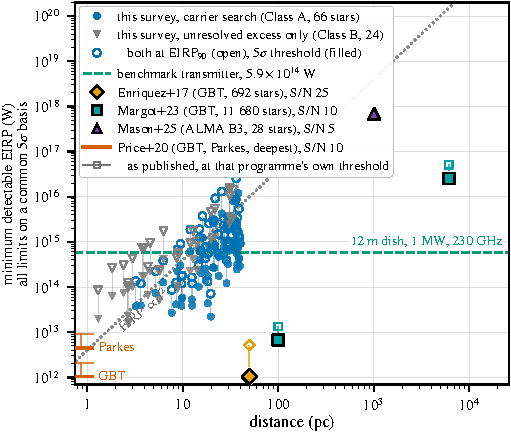
\includegraphics[width=\columnwidth]{figures/eirp_context_a.pdf}\\
{\footnotesize (a)}\\[4pt]
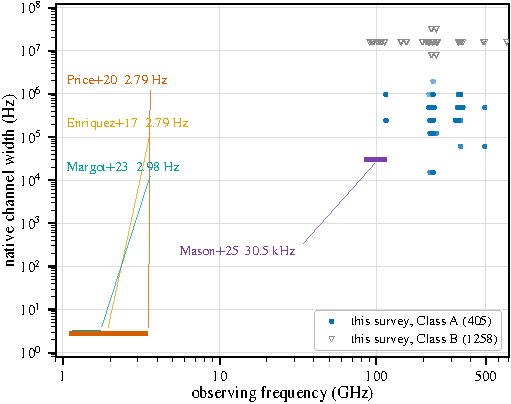
\includegraphics[width=\columnwidth]{figures/eirp_context_b.pdf}\\
{\footnotesize (b)}
%% ★★★ v4.26 (r25-captions): 16 PRINTED LINES -> R1 §7's limit of about six.
%% MOVED into \S\ref{sec:intro}, where Fig.~1 is discussed, and carrying with
%% it three macros THIS CAPTION WAS THE ONLY CITATION SITE OF -- \LtChanSpanDex,
%% \LtChanNarrow, \LtChanWide -- and a fourth, \NgNDecBOnly: the native-channel
%% span and what it means for comparing two programmes; "no limit plotted
%% carries a confirmation criterion"; the grey triangles constraining an
%% unresolved excess and not a carrier; and "the only symbols carrying
%% measured completeness".  Deleting instead of moving would have let
%% retire_macros.py take four numbers out of the paper in silence.
%% DELETED, because the drawn panels already carry it or \S1 already says it:
%% "each published value kept beside its rescaled one" (\S1 states exactly
%% that of the rescaling) and the list of what the panels label, which they
%% do label -- \BenchDiam keeps two citation sites elsewhere.
\caption{Where this survey sits among published radio technosignature
searches, on Table~\ref{tab:litthresh}'s common $\LtCommonSnr\sigma$ basis
(\S\ref{sec:intro}). \textbf{(a)} Minimum detectable EIRP against distance;
this survey's deepest window per star -- blue, the carrier search; grey,
coarse channels only; filled, the bare threshold; open,
$\mathrm{EIRP}_{90}$. \textbf{(b)} Native channel width against sky
frequency (filled, Class~A; open, Class~B).}
\label{fig:context}
\end{figure}

%% ★ Figure 1's caption was 30 printed lines, 1848 characters, the longest in
%% the main text; the referees asked for about 60 per cent off, and it is now
%% 17 printed lines / 1023 characters, measured by capmeasure.py.
%% WHAT WENT: the colour legend (orange/aqua/violet/left-edge ticks, grey
%% dotted, green dashed) -- "the panel labels already carry the legend", and
%% they do, the panels print Parkes, GBT, Price+20, Enriquez+17,
%% EIRP propto d^2 and "12 m dish, 1 MW, 230 GHz"; the sentence re-explaining
%% the rescaling; and the "Compare the hollow markers with this survey's
%% filled ones" aside.
%% WHAT STAYED, because each is a caveat and not an explanation: the native
%% channel span (a limit is only a limit for a signal narrower than the
%% channel that set it), the Class B triangles constraining an unresolved
%% excess and NOT a drifting carrier, completeness measured only for this
%% survey's open symbols, and no confirmation criterion anywhere on the
%% figure.  Two caveats MOVED into §1 so each survives exactly once: the
%% matched-false-alarm qualification, which §1 states where the rescaling is
%% described, and "excludes atmospheric decorrelation", which Table 3 defines
%% as the meaning of "nominal".
%% ► Enriquez2017 and Price2020 keep citation sites elsewhere, so dropping
%% the colour legend does not orphan a bibitem.
%%
%% Housekeeping. The two-symbol convention on panel (a) -- bare 5 sigma
%% filled, EIRP_90 open, joined -- is set by make_fig_context_v410.py.
%
\section{The sample}
\label{sec:sample}

This search covers \NWindows{} spectral windows toward \NStars{} stars in
\NSystems{} systems within 40\,pc. They are drawn from \NEB{} public ALMA
execution blocks and \TotalDataTB\,TB of raw data, put through one
pipeline: \StTelHours\,h of telescope time, and \LdgCensusHours\,h summed
over windows. That set is the \emph{primary census}: every
sensitivity, every expectation and every limit here is computed over it, and
so are \MtCrossACen{} of the \EvNCrossRaw{} threshold crossings this paper
reports. \LdgNCrossB{} more are coarse-channel crossings of the same census,
all of them in the one execution block that fails the data-quality criterion
of \S\ref{sec:summary}, and they are reported apart for that reason and not
because they fall outside it. The remaining \CeNTailCross{} lie in the
\emph{archival tail}: blocks searched after the sweep that fixed the census
was closed, toward stars the census already holds, whose windows are not
tabulated window by window here and enter no expectation. Three further sets
were searched and enter no census statistic either -- the \emph{archival
extension}, a larger harvest of blocks toward the same stars; a
\emph{hold-out}, set aside by the identifier rule of
Appendix~\ref{sec:heldout} and searched as an additional sample; and a
control beyond 40\,pc -- and each is reported with its own counts where its
result is (\S\ref{sec:holdoutsearch}).
Table~\ref{tab:blockledger} names them in rows that sum, and
Table~\ref{tab:counts} resolves every count of windows, crossings and systems
into the set it is counted over.

\emph{Star} means one stellar component, \emph{system} a bound group
counted once however many of its components were observed, and \emph{target}
one ALMA pointing.

The census is two experiments, divided on native channel width, which is
what the search statistic and the completeness calibration both depend on.
\emph{Class~A} is the \NWinA{} fine-channel windows toward
\LdgClassAStars{} stars in \NSysClassA{} systems, and every sensitivity and
exclusion quoted here refers to them unless stated otherwise;
\emph{Class~B} is the remaining \NWinB{} coarse-channel windows, which
support a secondary search for an unresolved spectral excess. The division
is unambiguous because the channelisation of the sample is bimodal: the
widest fine channel is \ScChanFineMaxMHz\,MHz and the narrowest coarse one
\ScChanCoarseMinMHz\,MHz, a factor of \ScChanGapFac{} with nothing between
them. Whether a window can also discriminate a drifting carrier is a
separate question, and \S\ref{sec:statistic} answers it: \EtaDriftAOk{} of
the \NWinA{} can, \EtaDriftALo{} cannot.

Every inclusion criterion was applied by query. A star enters
if its Gaia~DR3 parallax is at least 25\,mas, measured to better than
\PlxAdqlPct{} per cent, and if its proper-motion-corrected position at the
observation epoch falls inside the quoted field of view of at least one
public execution block. Distances are direct inversions, $d=1/\varpi$, and
the star need not sit at the pointing centre. One further rule applies to the
window and not to the star: a window is kept only where the primary-beam
response at the star is at least \BmFloorResp, the offset at which the
Gaussian adopted here and the response of a blocked circular aperture
part by \BmFloorTolPct{} per cent. It removes nothing, in the census or in
the archival coverage beyond it: the furthest window from a pointing centre
lies at \ExCWorstExt\,$\lambda/D$ against a limit at
\BmFloorC\,$\lambda/D$, so the limit does not stand clear of the
distribution, and the windows it is nearest are the off-axis ones on
$\epsilon$~Eridani, which the survey searches.
The precision clause never binds: the worst fractional parallax
error among the stars searched is \SfPlxWorstPct{} per cent. The query returns
\NCensus{} work-list entries; the quoted field of view is optimistic, and
only \NGenuinelyCovered{} of those stars are in fact contained by a public
field, of which \NStars{} yielded a searchable window. One target has no
catalogue name -- a serendipitous field star that appears throughout as
\BkAlmaName, Gaia~DR3 \BkAlmaGaia, an \BkAlmaSpType{} dwarf at
\BkAlmaDistPc\,pc with no measured systemic velocity.

Disc, planet and colour enter as descriptive metadata only. One exclusion,
though, is a property of the catalogue and not of the sky: a Gaia~DR3
parallax needs a Gaia~DR3 source, and the brightest stars have none. Every
one of the \BsNBright{} stars in this volume brighter than \BsBrightMag{}
magnitude is absent from DR3 astrometry, and so is a steady
\BsGapFaintPct{} per cent of every magnitude bin below Hp~\BsGapMagCut,
which saturation does not explain. Together \BsNGap{} of the \BsNVol{} Hipparcos stars whose own parallaxes
meet the criteria above never reached the work list: \BsGapNBright{} of them
brighter than Hp~\BsGapMagCut{} and \BsGapNFaint{} fainter. Of these,
\BsNAlmaWord{} lie inside a public field of view -- \BsStarList{} -- and
hold \BsNWinA{} fine-channel and \BsNWinB{} coarse-channel windows, amounting
to \BsRawTB\,TB of raw data in \BsNEB{} execution blocks, none of it searched
here -- Sirius~A among them, since the \BsSirNEBWord{} blocks that put
Sirius~B in this census are pointed at it. A search of
this volume should admit these stars on Hipparcos astrometry where Gaia has
none.

Two removals act on windows and not on stars and account for the whole
difference between the \LqNExport{} rows the extraction wrote and the
\NWindows{} retained: \NDup{} repeated rows of one window, and \NDefect{}
lying more than \LqDefectCut{} times below the sample median in
$\sigma\sqrt{t_{\rm on}\Delta\nu_{\rm ch}}$ and so not measuring the sky. The
primary-beam limit above removes none, and no integration-time cut was
applied.

\subsection{The archival selection}
\label{sec:bias}

This sample was not designed: it is whatever previous ALMA programmes
happened to observe among the stars Gaia~DR3 catalogues, and
\PctDiscProposal{} per cent of the stars searched were targeted under a
debris-disc or planet-formation proposal. Table~\ref{tab:selfunc} measures
the bias against a volume-limited reference census of which the searched
stars are a subset, classifying both columns by one rule so that every ratio
below -- the searched column fraction over the census column fraction, above
one for over-representation -- is like against like. Both columns are the
same Gaia~DR3 selection --
$\varpi>0$, $\sigma_\varpi/\varpi\le\SfPlxCutDec$ and $1/\varpi\le40$\,pc,
\SfCensusN{} objects -- and the looser \PlxAdqlPct{} per cent the query above
applies selects exactly the same objects, so the two cuts are one selection
and not two. The one rule is colour: BP$-$RP sets the class, and the absolute
$G$ magnitude separates the degenerates that colour alone would place among
the A~stars. It reaches \SfCensusNCol{} census objects, \SfCensusColPct{} per
cent of them, and \SfNClassified{} of the \SfNStar{} searched stars, the
other \SfNNoColour{} carrying no Gaia BP or RP photometry. Both columns are
Gaia-defined, so neither contains the bright stars above and the ratios are
internally consistent without them.

Distance is the dominant selection effect. Stars within 5\,pc are
over-represented by a factor \SfTopRatio, and the enhancement falls
monotonically with distance to a factor of two \emph{under}-representation
beyond 30\,pc. Colour comes second: A~stars are over-represented by about
\SfARatio{} and F and G stars by factors of three, because those are the
stars with bright debris discs. For the A~stars that factor is a floor,
because the catalogue requirement is itself colour-selective: it removes
\BsNEarly{} of the \BsNEarlyVol{} stars in the volume as blue as an A~star,
\BsEarlyRatio{} times its rate among all the others. M~dwarfs are depleted
--
\SfMSearched{} of the \SfNStar{} searched stars are M~dwarfs, a factor
\SfMRatio{} of their share of the reference census, and only
\SfMClassAStars{} of them carry fine-channel coverage at all. Coverage is also concentrated:
\ConcThreeWin{} of the \NWindows{} windows come from \ConcThreeSys{}
systems. No statement in this paper is therefore an occurrence rate for the
solar neighbourhood, and the selection acts hardest on
exactly the targets a designed search would pick: of the \CsIntNRow{} sample
systems within 15\,pc with a confirmed planet, \CsIntNoClassA{} carry no
Class~A coverage and so no drift-resolving limit.

%% GENERATED by selfunc_v411.py -- do not hand-edit.
\begin{table}
\centering
\scriptsize
\setlength{\tabcolsep}{4pt}
\caption{Selection function of the 90 searched stars against the volume-limited Gaia~DR3 census of \S\ref{sec:bias}. ``Ratio'': the searched over the census column fraction.}
\label{tab:selfunc}
\begin{tabular}{@{}lrrr@{}}
\toprule
Property & Census & Searched & Ratio \\
\midrule
\multicolumn{4}{@{}l}{Distance} \\
\quad $d\le5$\,pc & 48 (0.3\%) & 13 (14.4\%) & 52.9 \\
\quad 5--10\,pc & 240 (1.4\%) & 13 (14.4\%) & 10.6 \\
\quad 10--20\,pc & 2069 (11.8\%) & 18 (20.0\%) & 1.7 \\
\quad 20--30\,pc & 5391 (30.7\%) & 19 (21.1\%) & 0.7 \\
\quad 30--40\,pc & 9818 (55.9\%) & 27 (30.0\%) & 0.5 \\
\midrule
\multicolumn{4}{@{}l}{Colour class$^{a}$} \\
\quad A & 61 (0.4\%) & 5 (6.2\%) & 17.2 \\
\quad F & 473 (2.8\%) & 8 (10.0\%) & 3.6 \\
\quad G & 978 (5.8\%) & 15 (18.8\%) & 3.2 \\
\quad K & 2221 (13.2\%) & 11 (13.8\%) & 1.0 \\
\quad M & 13\,082 (77.8\%) & 41 (51.2\%) & 0.7 \\
\midrule
\multicolumn{4}{@{}l}{Other axes} \\
\quad Confirmed planet hosts$^{b}$ & 26 (15.5\%) & 24 (26.7\%) & 1.7 \\
\quad White dwarfs$^{a}$ & 463 (2.7\%) & 8 (9.1\%) & 3.4 \\
\quad Searched stars / systems & -- & 90 / 83 & -- \\
\bottomrule
\end{tabular}

\smallskip
{\footnotesize $^{a}$Colour bins, not MK types. The boundaries are the colours at which the census's own temperature--colour relation crosses 7500, 6000, 5300 and 3900\,K: BP$-$RP $<0.36$ for A, 0.36--0.72 for F, 0.72--0.95 for G, 0.95--1.77 for K and $>1.77$ for M. Over the 8594 census objects that also carry a Gaia temperature the two classifications agree for 98 per cent, and every disagreement is between neighbouring bins. A star is counted as degenerate when it lies more than 4\,mag below the main sequence measured from the census itself: the two sequences are separated by 5 to 8\,mag here, so moving the cut by a magnitude either way changes the count by under 3 per cent. The five classes are normalised over the 80 non-degenerate searched stars and the 16\,815 non-degenerate census objects, and the degenerate row over the 88 classified searched stars and the 17\,278 classified census objects, which is the same rule in both columns.\\ $^{b}$Both columns are the same positional join, of the 168-entry ALMA-covered work list and of its searched subset, to the NASA Exoplanet Archive \texttt{pscomppars} table accessed 2026 October 4. The 24 searched hosts carry 51 confirmed planets, 22 of the 24 surviving the deuterium-burning mass limit; the Gaia census carries no planet information, so the census column in this row is the work list and not the 17\,566-object Gaia census.}
\end{table}


%% fig:funnel DELETED: it drew the three counts the sentence above it
%% already carries, so it joined the prose instead of replacing it.  The
%% artwork is online material (figures_diagnostic/selection_funnel.pdf).

\subsection{Frequency coverage and archival scope}
\label{sec:coverage}

The Class~A experiment covers $\Delta\nu_A=\DnuA$\,GHz of unique sky
frequency, and that coverage is sparse: \DomAIslands{} disjoint islands
between \DomAFreqLo{} and \DomAFreqHi\,GHz instead of a band, so those
endpoints bound where observations exist and not what was covered. With the
coarse-channel windows the archival coverage is \DnuAB\,GHz in
\UnionIntervals{} intervals, of which \SearchedUnionGHz\,GHz survives the
molecular-line mask of \S\ref{sec:method}. Fig.~\ref{fig:waterfall} shows the
distribution: a transmitter between the islands was never observable here,
whatever its power.

The archive is not exhausted either. \LdgExtScope{} further blocks lie inside
the same query and were unprocessed when the census was frozen;
Table~\ref{tab:blockledger} accounts for every one of them row by row,
including the \LdgExtEB{} reported here as repeat epochs. The largest single
gap is the \FateNoCal{} blocks whose raw visibilities
the archive holds but never pipeline-calibrated, \FateNoCalGB\,GB in all; no
effort of ours would close that.

\begin{figure*}
\centering
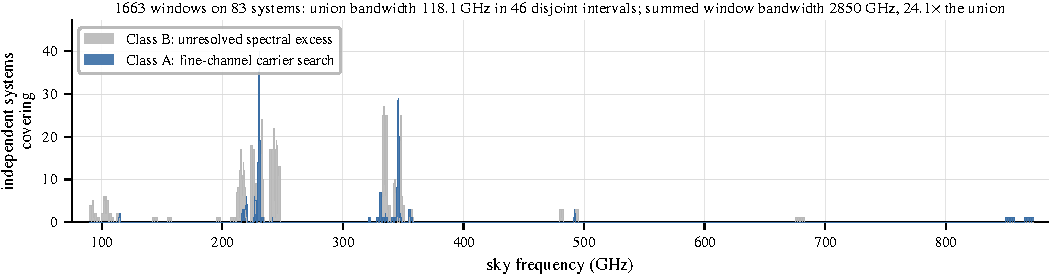
\includegraphics[width=0.99\textwidth]{figures/coverage_waterfall.pdf}
\caption{Where this survey searched: the number of independent systems
covering each sky frequency -- blue the fine-channel carrier search
(Class~A), light grey the coarse-channel spectral-excess search (Class~B).
Curves step at the searched window edges themselves, so an interval narrower
than a plotted pixel still appears. The summed window bandwidth is
$\GrossOverUnion\times$ the union.}
\label{fig:waterfall}
\end{figure*}

%% Floats that belong elsewhere: tab:blockledger is in Appendix A (its
%% headline rows are in the prose above, so the cross-reference is not a
%% pointer with no numbers beside it); tab:interesting is neither typeset nor
%% distributed -- r15-deposit, 2026-10-08: there is no deposit, so if its rows
%% are wanted by a reader they have to be printed; tab:searchspace is deleted, nothing having cited
%% it, and its counts, unions, channel widths and drift range are all
%% elsewhere in the paper.
%% Carried forward to the numbers owner: tab_interesting.tex is still
%% generated but is not in make_all.sh, and its planet column should read the
%% dated NASA Exoplanet Archive extract selfunc_v411.py uses so that one
%% definition of "confirmed planet" serves both tables.  Two display defects
%% belong in star_alias.designation: Barnard's Star prints as a SIMBAD
%% identifier with the "NAME" prefix stripped, and BD+05 1668 would read
%% better with its GJ alias beside it.
%
\section{Data and methodology}
\label{sec:method}

The search looks for one kind of signal: an unresolved carrier at the
star's own position, narrow compared with a single correlator channel, and
drifting in sky frequency because the transmitter accelerates along the line
of sight. Over a long track its power is spread across many channels, so a
search that treats each channel on its own will miss it. The analysis therefore \emph{de-drifts} the data before it measures them:
each integration's spectrum is shifted to follow a trial drift rate, and only
then are they added together.

\subsection{The de-drifted search statistic}
\label{sec:statistic}

Each window's dynamic spectrum is stacked along every trial drift rate
$\dot\nu$. The search statistic is the largest stacked signal-to-noise
ratio anywhere on the resulting channel$\times$drift grid,
%
\begin{equation}
T(\mathbf{x})=\max_{\dot\nu,\;\nu}\;
\frac{\sum_{t} I\!\left(\mathbf{x},t,\nu+\dot\nu t\right)\big/\sigma^{2}(t,\nu)}
     {\left[\sum_{t}1\big/\sigma^{2}(t,\nu)\right]^{1/2}},
\label{eq:tstar}
\end{equation}
%
where $I(\mathbf{x},t,\nu)$ is the spectrum at sky position $\mathbf{x}$
in integration $t$ and channel $\nu$, and $\sigma(t,\nu)$ is the noise scale
there. Equation~\ref{eq:tstar} is the matched filter for a constant-drift
carrier: a drift-aligned, inverse-variance-weighted stack of the calibrated
intensities along the track, divided by the noise of that stack, so $T$ is an
absolute signal-to-noise ratio and not a local contrast. In Equation~\ref{eq:tstar} the time $t$ runs from the first integration of the
observation, so the frequency $\nu$ that labels a track is the one a carrier
would occupy at the start of that block, and a repeat epoch is read at the
cell the same convention fixes (\S\ref{sec:etacrv}).
The noise scale is the median absolute deviation
across \NCtrl{} control positions at each integration and each channel,
scaled to its Gaussian-equivalent standard deviation: local in time and
frequency, global in position, and shared by the star and every control.
They lie, from a fixed seed, in an annulus set by each block's own
synthesised and primary beams: the field read over is that block's primary
beam.
The statistic is evaluated at one position at a time, identically at the
star and at each control, which is what makes the two comparable.
$T_\star$ denotes its value at the star.

Spectra are extracted at the star's apparent position, never from images.
For each integration and each native channel the pipeline forms the weighted
vector average of the phase-shifted visibilities, in total intensity: the
mean $I=(XX+YY)/2$ of the two parallel-hand correlations. That average is the
dirty-map value at the extraction position -- an amplitude, not a
deconvolved flux density, so in a field with extended emission it is not a
point-source measurement. The correction for the displacement of that
amplitude is measured and not assumed: a carrier injected into the same
visibilities and recovered at both the catalogue and the apparent position
returns the normalised dirty beam on that block's own baselines, and exceeds
the model at the larger displacement, so a limit corrected by it is
shallower than it need be (Appendix~\ref{app:pbresp}).
The data are used as the archive delivered them,
through ALMA's own calibration and quality assurance, with their flagging
carried through, every delivered channel searched, and no regridding,
deconvolution or edge trimming. A per-integration median along the
\emph{frequency} axis removes the continuum; it removes a level and not a
shape, and no median is taken along time, so no feature narrow against the
band can be removed by it. One
subtlety matters for every power quoted below: the delivered channels are
smoothed, so a channel's effective noise bandwidth is not its separation
and flux density times channel width is not yet a radiated power. A
response correction computed from the correlator's own channel shape
supplies the difference (Appendix~\ref{app:conventions}).

One convention holds everywhere in the paper. The search runs on the
topocentric sky frequencies ALMA delivered, and every drift rate quoted is
the apparent one at the telescope, which is what the data contain and what
a reader can recompute from the archived channel axes. Two steps need the
star's own frame and both take it: a crossing is compared with the line catalogue, and a repeat epoch is read
at the \emph{predicted cell} -- the single channel, at a single drift rate,
where the first epoch's own fit says a carrier should be. Both take that
frame by correcting each block's frequency axis for the Earth's motion at
that epoch and then for the star's systemic velocity, which is the
catalogued radial velocity from SIMBAD \citep{SIMBAD2000}, queried on
\SimbadQueryDate, and zero where the
catalogues give none. One star departs: toward $\beta$~Pic the adopted value
is \BpRecVsys\,km\,s$^{-1}$, the stellar radial velocity adopted in the ALMA
CO analysis of its disk \citep{Matra2017}, which this survey's own blocks
reproduce to \BpRecVsysSpread\,km\,s$^{-1}$ in the barycentric frame. The
catalogued value is lower by \BpRecVsysGaiaDiff\,km\,s$^{-1}$, in the sense
and of the size of the template-mismatch offset the \textit{Gaia} pipeline
documents for stars this hot and leaves in its archive \citep{Blomme2023}.

Two power quantities carry the main text, both defined in
Table~\ref{tab:quantities}: the trigger level $P_{\rm trig} = 4\pi
d^{2}S\,\Delta\nu$ at distance $d$, for a carrier that makes $T_\star$ reach
$T_{\rm trig}=\StageNullTrig$ in one native channel of width $\Delta\nu$,
and the sensitivity $\mathrm{EIRP}_{90}$. The second is measured, not
assumed: synthetic carriers of known amplitude were injected into
calibrated visibilities and recovered through the unmodified pipeline.
Three campaigns did that, one for each stage of the chain the completeness
depends on: the trigger completeness itself, on \MkInjCompWin{} of the
\MkInjCompDenom{} fine-channel windows injected directly and on
\SensNToneCoarse{} carriers of the coarse class; the cost of the spatial
rank, on \SelNTone{} carriers over \MkInjSelUnit{} of \MkInjSelTotal{}
attempted block--window configurations; and the primary-beam correction, on a
third set of \MkInjBeamUnit{} scored units, \MkInjBeamShared{} of them also
among the directly injected windows. Between them they span both ALMA arrays,
four bands and the sample's full range of channel widths. Every limit quoted in
this paper is the $\mathrm{EIRP}_{90}$ of its own window, given to two
significant figures beside its native channel width, except the
bare-threshold comparisons of \S\ref{sec:intro} and
Fig.~\ref{fig:context}(a), which are labelled as such; the measured
completeness is \S\ref{sec:pninetysel} and its error
budget is Table~\ref{tab:p90budget}. Two comparisons bear on the amplitude
scale and they are not the same kind of check. An independent reduction of the same AU~Mic visibilities is reproduced to
\PxJanRatio\,$\pm$\,\PxJanRatioErr. That tests the extraction and not
ALMA's flux transfer, an error in which would appear in both reductions
alike. The external comparison is with the published quiescent flux density
of $\epsilon$~Eridani, recovered to
\PxEpsRatio\,$\pm$\,\PxEpsRatioErr{} \citep{Burton2022} and so a
\SbEpsPct\,per cent measurement. The absolute scale is therefore carried at ALMA's own band-dependent
accuracy specification. The sample as a whole carries $\pm\BudComb$ per
cent, and the \BudNHiWin{} Class~A windows in
\BudHiBandWord~\BudHiBands, at \BudHiGHzList\,GHz, carry
$\pm\BudCombWorst$.

The drift range searched is bounded by an acceleration, not by a
frequency. Drift rate and line-of-sight acceleration are one quantity in
two sets of units,
%
\begin{equation}
\frac{\dot\nu}{\nu}=\frac{a_{\rm los}}{c}
\qquad\text{and so}\qquad
a_{\rm los}=\frac{c\,\dot\nu}{\nu},
\label{eq:accel}
\end{equation}
%
so a ceiling expressed as $\dot\nu/\nu$ is the same physical limit in
every band. The default ceiling is
\DriftCeilLo--\DriftCeilHi\,Hz\,s$^{-1}$\,GHz$^{-1}$, the acceleration of a
transmitter orbiting a solar-type star at a few hundredths of an au: the
\citet{Mason2025} fiducial with a threefold margin, widened for a confirmed
exoplanet host whenever the innermost known planet demands more, and
\AccelSheikhPct{} per cent of the \AccelSheikhNHz\,nHz that
\citet{Sheikh2019} recommend for a general search, whose figure is set by the
closest observed exoplanet orbit. As an acceleration that default ceiling is
\AccelCeilMed\,m\,s$^{-2}$, which is also the median over the Class~A
windows, and it rises to \AccelCeilMax\,m\,s$^{-2}$ on the \AccelNWide{}
\AccelWideStar{} windows. The grid is uniform in $\dot\nu$ and fine
enough that a carrier midway between two trials loses no more than
\DriftGridFineHalf{} of a native channel over the longest track, and runs
from the negative ceiling to the first trial at or beyond the positive one
(Appendix~\ref{sec:edge}).
\textbf{The survey does not constrain a transmitter whose apparent
acceleration exceeds that range}, and three cases put one there: a
deliberately chirped carrier, which is in any case not distinguished from an
accelerating platform; a transmitter not bound to a known planet; and the
sum of orbital and rotational acceleration, which share the one budget, so a
transmitter on a rapidly rotating planet can exceed the ceiling on its spin
alone -- $\beta$~Pictoris~b, the fastest rotation measured for any
planetary-mass object and orbiting one of the stars searched here,
corresponds to \AccelBpicRotNHz\,nHz \citep{Sheikh2019}. For the most
demanding known case, transiting TRAPPIST-1~b, \TrapPhaseHi{} per cent of the
orbital phase lies above the default ceiling, and its maximum line-of-sight
acceleration equals the widened grid used on that star's own windows to
within the $\pm\TrpAmaxPct$ per cent its host's mass and orbit are known to,
so the fraction of phase above that grid is anywhere between nothing and a
sixth (Fig.~\ref{fig:accel}). That figure draws three reference accelerations
beside the ceiling: \AccelWorstName{} and \AccelSecondName{} at
\AccelWorstVal{} and \AccelSecondVal\,m\,s$^{-2}$, the two most demanding
known planets of any target, the second of them searched in coarse-channel
windows only; and a Jupiter's equatorial rotation at
\AccelJupRot\,m\,s$^{-2}$, which alone would spend \AccelJupPct{} per cent of
the budget.

\begin{figure}
\centering
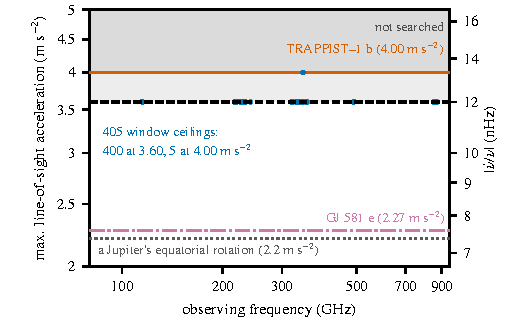
\includegraphics[width=\columnwidth]{figures/drift_acceleration.pdf}
%% ★★★ v4.26 (r25-captions): 11 PRINTED LINES -> R1 §7's limit of about six.
%% TEN macros had this caption as their ONLY citation site -- \AccelCeilMed,
%% \AccelCeilMax, \AccelNWide, \AccelWideStar, \AccelWorstName,
%% \AccelSecondName, \AccelWorstVal, \AccelSecondVal, \AccelJupRot,
%% \AccelJupPct -- so every one of those clauses had to MOVE and none could
%% be deleted: retire_macros.py would otherwise have taken ten numbers out of
%% the paper without a gate going red.  They are now two sentences of
%% \S\ref{sec:statistic} above, beside the ceiling they qualify.  The caption
%% keeps what reads the panel: what a point is, both axes, the shading, and
%% that the horizontal lines are reference accelerations.
\caption{What the drift search reaches, as a physical selection function: the
drift ceiling of each of the \NWinA{} Class~A windows (points), by
Equation~\ref{eq:accel}, against observing frequency, with the unsearched
region shaded and the same quantity as a fractional drift rate on the right.
Horizontal lines are the reference accelerations of \S\ref{sec:statistic}.}
\label{fig:accel}
\end{figure}

Only part of the archive can carry a drift search at all, and the two
classes reported here are that division (Table~\ref{tab:quantities}).
Channelisation in the sample is bimodal with an empty gap between the
modes, so the split is unambiguous -- but it is a split on channel width,
and the criterion that decides whether a window can discriminate a drifting
carrier at all is whether the maximum searched drift crosses of order one
channel or more over the on-source track, $\eta_{\rm drift} =
|\dot\nu_{\max}|\tau_{\rm track}/\Delta\nu_{\rm ch} \gtrsim 1$. The two do
not partition the survey identically: \EtaDriftAOk{} of the \NWinA{} Class~A
windows satisfy it and \EtaDriftALo{} fall below, each of
them a track of \ScLoTauLoS--\ScLoTauHiS\,s against a class median of
\ScLoTauMedAllMin{} minutes, so it is the short track and not the channel
that fails them; the released per-window catalogue carries $\eta_{\rm
drift}$ for every window and so names them.
\EtaDriftBHi{} of the \NWinB{} coarse windows meet the
criterion and stay in Class~B, because meeting it is necessary for drift
discrimination and not sufficient: their channels are \ScBhChanMHz\,MHz, the
whole searched range moves a carrier only \ScBhEtaLo--\ScBhEtaHi{} of one,
and a channel-confined carrier there is diluted by \ScBhDiluteFac{} times
the median fine channel, which is the Class~B limit measured for them by
injection. Nothing is hidden by that choice: all \ScBhNSys{} of their
systems already carry fine-channel coverage and none of the
\EtaDriftBHi{} holds a crossing, so no system and no crossing turns on it;
they would add \ScBhNewBandGHz\,GHz of frequency outside the Class~A
union.

\subsection{From a crossing to a confirmed signal}
\label{sec:summary}

Every window passes through the same three tests in the same order, and
three words name what comes out of them: a \emph{crossing}, an
\emph{unattributed crossing} and, had one survived, a \emph{confirmed
signal} (Fig.~\ref{fig:chain}), each defined once in
Table~\ref{tab:quantities} and used in no other sense. There is no fourth
test, and none of the three is a significance test. Coincidence with a
catalogued transition is a flag and not a disposal, so all \CnCross{}
crossings continue past it, and the spatial rank and the visibility fit are
diagnostics attached to the middle level that decide nothing. Every count in
that figure is read from the ledger, which lists every crossing the search
produced, including those in the archival-tail blocks and in the
quality-failing block that no expectation is computed over, so the figure,
the ledger and the text cannot disagree. The counts drawn are the primary
crossings, one to a window: the \CkNSecondary{} secondary crossings of
\S\ref{sec:technosearch} enter the same three levels, and
\CkNSecUnattrWord{} reach the second, none the third. The reserved hold-out
is drawn as a separate branch because a transmitter in it would matter
whatever its calibration role.

%% ★ minor 3 (figure numbering).  This float was in Sec. 5, but Fig.~\ref{fig:chain}
%% is first cited HERE, in Sec. 4.2, before Figures 4-6 are cited at all, so the
%% figure numbers ran out of citation order.  LaTeX numbers a float where its
%% environment is read, so the fix is to read it here.  Moved by the figures
%% owner; its caption and its counts are unchanged.
\begin{figure}
\centering
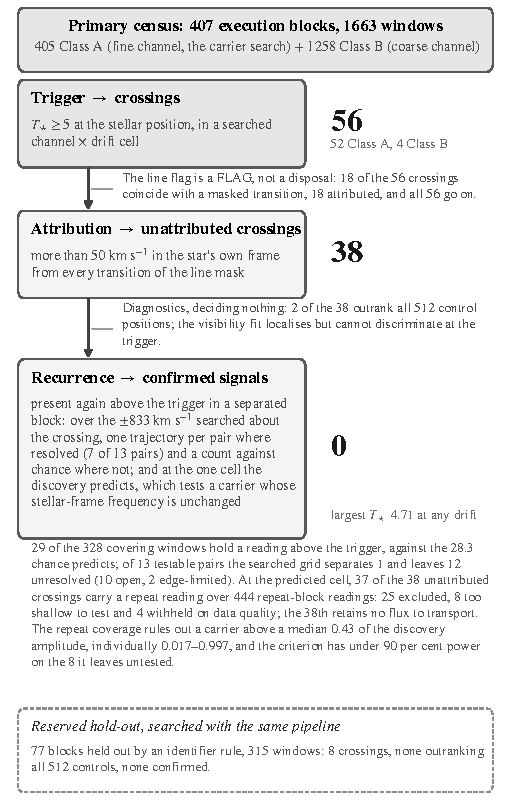
\includegraphics[width=\columnwidth]{figures/chain_v412.pdf}
%% ★★★ v4.26 (r25-captions): 16 PRINTED LINES -> R1 §7's limit of about six.
%% Two clauses were already DRAWN inside the figure -- the line flag "not a
%% disposal" and the diagnostics "deciding nothing" -- and the three terms are
%% defined once in Table~\ref{tab:quantities}, which is what licenses dropping
%% their glosses here.  Everything else went into \S\ref{sec:summary}'s own
%% paragraph above, carrying \CnCross, \CkNSecondary and \CkNSecUnattrWord
%% with it: this caption was the only citation site of \CnCross and
%% \CkNSecondary, so deleting rather than moving them would have let
%% retire_macros.py take two counts out of the paper silently.
\caption{The detection logic, with the count at each level. Three levels and
no more: a \emph{crossing} is an event requiring investigation, an
\emph{unattributed crossing} a target for follow-up, and a \emph{confirmed
signal} would be a detection. All three are defined in
Table~\ref{tab:quantities}, and \S\ref{sec:summary} gives the provenance of
every count drawn.}
\label{fig:chain}
\end{figure}

\begin{enumerate}[label=(\roman*),leftmargin=1.9em,itemsep=3pt,topsep=3pt,parsep=0pt]
\item \emph{Trigger $\to$ a crossing.} The quantity is $T_\star$, the
de-drifted statistic of Eq.~\ref{eq:tstar} read at the stellar position; the
criterion is $T_\star\geq T_{\rm trig}=\StageNullTrig$ in at least one
channel$\times$drift cell. $T_{\rm trig}$ is a trigger
threshold and not a detection significance: $T$ is not shown to follow any
standard distribution under the null, so the level carries no tail
probability, and a window holds between \TuCellsLo{} and $\TuCellsHi$ of
those cells, so one level buys very different protection in a coarse
single-pointing window and in a finely channelised one on a long track. Every
cell that reaches the level is recorded, not only the largest in each window,
because a carrier is masked as effectively by a noise excursion as by a line.
A crossing establishes only that it goes on to the next two tests.
\item \emph{Line attribution $\to$ an unattributed crossing.} The quantity
is the crossing's velocity offset from the nearest transition of a
molecular-line catalogue, evaluated in the star's own rest frame; the
criterion is $\pm\MaskHalfKms$\,km\,s$^{-1}$. The line catalogue is a
single database query, made on \MkListDate{} and repeatable as it stands.
Each crossing's \emph{disposition} -- the account this paper
gives of what it is -- rests on the physical evidence set out beside it.
The half-width follows the Keplerian line-of-sight
velocities of gas
surviving beyond a few au, with margin for the systemic velocity. A crossing
inside that window is \emph{attributed} where the species is one that such
systems are known to carry: a coincidence with a catalogued transition makes
an astrophysical origin far more likely than a transmitter, the more so
where a second transition of the same species or known circumstellar
emission is present. A further \SoNCrossWord{} crossings coincide with a
species no debris disc has been shown to carry; their offsets are reported
and they are counted as unattributed (Appendix~\ref{app:linemask}).
A coincidence is in any case a statement about a catalogue and not a
property of a frequency, so this is an attribution, and
every crossing goes on to the recurrence test whichever side of the
window it falls, wherever a later block covers the frequency. The
window's price is that the survey constrains nothing inside it
(Appendix~\ref{app:linemask}).
\item \emph{Independent recurrence $\to$ a confirmed signal.} The quantity is
$T_\star$ at the cell the first epoch predicts, read in another execution
block of the same star at a single drift rate after the frame correction of
\S\ref{sec:statistic}; and the criterion is that it reach the trigger again.
That cell is the one a carrier would occupy at the start of that block,
which is where the de-drift of Equation~\ref{eq:tstar} is anchored, so the
criterion is met only by a carrier whose stellar-frame frequency at the two
epochs agrees to within half a native channel: it has the power to reject a
carrier that has moved further and none to accept one. The
recovering block must be a \emph{separated} one: an execution of a different
observing session, \emph{and} more than \EpSep{} day from the first. One
reason covers both halves. Blocks of one session share calibrators,
atmosphere, correlator setup and interference environment, and the residual
of \S\ref{sec:bdblock} is what that can produce -- which holds for two blocks
of one session however far apart they were executed, and \QfNPairDrop{} pairs
of blocks here are of one session and more than a day apart, the widest by
\QfSameSessMaxD\,d. So a recovery in any block of the discovery's own session
is a \emph{within-session repeat}, whatever the interval: necessary for a
confirmation and not sufficient for one. This is also the rule the
confirmability census of \S\ref{sec:confirmability} scores the archive on, so
the criterion and the scoring are one rule. It is a weak criterion, and the
archive's uneven temporal sampling is why: only part of the sample has epochs
separated well enough to apply it at all.
\end{enumerate}

\emph{Two diagnostics hang off the second test, and the word is exact: each
says which crossing deserves attention first, and neither decides anything.}
The first ranks $T_\star$ against the same statistic at that window's own
\NCtrl{} control positions (\S\ref{sec:statistic}), none of which
sits on the star; its lowest value, $1/(\NCtrl+1)$, means the star beat every
control. It is a ranking filter and not a significance test, because the
stellar and control positions are not demonstrably exchangeable: on
\HoWin{} reserved windows outside the census the stellar
rank has median \HoRankMed{} where one half is expected if the two were
interchangeable, and \HsIndRankMed{} over the \HsIndBlocks{} of those
blocks that share no observing session with a searched one; no parameter-free
correction for the annulus geometry restores an exchangeable
statistic (Appendix~\ref{app:radius}). It
also responds to compactness and not to origin, as $\beta$~Pictoris
shows: genuine carbon monoxide ranks below its own control ring there,
because the resolved disc lifts the ring along with the star. The second
diagnostic is a visibility-domain fit, which asks whether a crossing's
emission is at the stellar coordinates; it
%% ★★ v4.26 (r25-captions), FLAGGED AND REPAIRED, NOT INTRODUCED HERE.  This
%% sentence reached the built PDF as "...because a noise maxi-mum at the the
%% star (S4.5)." -- a doubled article AND a clause with no verb, so the
%% duplicated word was the only visible sign that something had been lost.
%% Removing the duplicate alone would have hidden the fragment instead of
%% fixing it.  The completion asserts nothing new: that the fit cannot tell a
%% noise maximum at the star from a source there at the trigger level is what
%% the first half of this same sentence says and what \S\ref{sec:vistest}
%% measures ("the fit excludes neither crossing: injected sources in the bin
%% these two occupy return Re/sigma = ...").  ►► IF THE ORIGINAL CLAUSE CAN BE
%% RECOVERED FROM AN EARLIER VERSION, PREFER IT TO THIS.
cannot discriminate at the trigger either, because at that level a noise
maximum at the star fits as a point source there
(\S\ref{sec:vistest}). Neither gates a
disposition, so neither is charged to the sensitivity.
Throughout, $p$ denotes a genuine significance level, and no probability
computed against the rank's own null is called one.

%% This heading said "and a rule fixed in advance says so", which the paper then
%% contradicts two appendices later: the condition was noticed in one block and
%% the criterion written afterwards.  The honest version says what the rule is
%% and leaves its provenance to the place that states it, so the two passages
%% cannot disagree.
\emph{One execution block is not a null, and a uniform rule says so.}
The comparison with the control positions needs each block's ensemble to behave
like noise, and a block fails when the median control statistic over its own
windows, scaled by the median of that quantity over its class, exceeds
\BqFactor{} that scale. Of the \BqNBlocks{} primary-census blocks, \BqNFail{} fails:
\BqFailBlock{} toward \BqFailStar, by a margin that does not depend on where
the line was drawn (Appendix~\ref{sec:blockquality}).
Its \BqFailNWin{} windows are all coarse-channel, so the Class~A
results are identical with it and without it: the same \BqWinACut{} windows
and \BqXrossACut{} crossings either way. But it holds \BqFailNCross{} of the
\NCross{} crossings, which is the survey's entire Class~B crossing
population (\S\ref{sec:bdblock}). The quality-passing data therefore hold
\EvNCrossQp{} threshold crossings, all of them Class~A. The criterion is
applied to blocks, and \BkFlagNCrossOther{} of those \EvNCrossQp{} lies in a
window the same diagnostic flags inside a passing block
(\S\ref{sec:bdblock}); it is counted here and withheld from the
amplitude-dependent tests, which is stated where each is made. The
\CkNCrossCenA{} in the primary census are the baseline every
expectation here is set against; the \CeNTailCrossWord{} in archival-tail blocks enter none of them.
The \BqFailNCross{} from the failing block are
reported in full in the ledger as the record of a block whose own control
ensemble does not satisfy the noise model the rest are compared with, and not
as crossings of the same standing (Appendix~\ref{app:falsealarm}).

Because a fixed threshold is not a fixed false-alarm rate, the number of
crossings expected by chance is computed window by window, from the
exceedance rate measured at each window's own control positions; the reserved
blocks then test the one assumption that makes, which is that a star behaves
like a control position in its own field (\S\ref{sec:trigunif}).

Three corrections precede the statistic: the extraction field is chosen so
that the star lies inside the delivered primary-beam field and not merely
inside the quoted field of view; the stellar position is propagated to the
observation epoch for proper motion, though not for the annual parallax or
for orbital motion, whose omissions are corrected window by window in
\S\ref{sec:pninetysel} and bounded for every component of a multiple in
Appendix~\ref{app:pbresp}; and on-source time is accounted per integration
from the
delivered exposure records and not from the scan intentions. That the
chain finds what it is meant to find is shown twice over, by the injected
carriers above and by $\beta$~Pictoris CO -- a real feature at a known
stellar position, recovered and localised in two transitions and
\NStageOneBpicEb{} execution blocks (\S\ref{sec:bpicval}).

\begin{table*}
\centering
\caption{The quantities and the three words this paper uses, defined once.
Every term below is used in this sense throughout and in no other. The
distinction the first three rows draw is the one the limits of
\S\ref{sec:pninetysel} turn on: a crossing is a single-epoch event, and a
confirmed signal needs a second and separated epoch that no sensitivity
supplies.}
\label{tab:quantities}
\small
\begin{tabular}{@{}p{0.145\textwidth}p{0.825\textwidth}@{}}
\hline
Term & Definition \\
\hline
Crossing &
A channel\,$\times$\,drift cell at the stellar position reaching
$T_\star\geq\StageNullTrig$ in one execution block; neighbouring channels
above the trigger belong to one crossing. The largest in a window is its
\emph{primary} crossing and any other a \emph{secondary} one, and because the
largest cell is the window's own statistic a secondary crossing exists only
where a primary one does. An event requiring investigation; no claimed
significance. \\
Unattributed crossing &
A crossing lying more than $\MaskHalfKms$\,km\,s$^{-1}$ in the star's frame
from every transition of the line catalogue. That is a reproducible frequency
coincidence; which coincidences are astrophysically plausible is a separate
judgement, stated with each one. A target for follow-up; not a detection. \\
Confirmed signal &
An \emph{unattributed} crossing recovered at the predicted stellar-frame
frequency and drift in a \emph{separated} block: an execution of a different
observing session, more than \EpSep{} day from the discovery block. A
recovery in the discovery's own session is a \emph{within-session repeat},
which a confirmation requires and which does not establish one. The criterion is
applied to every crossing, and a crossing coincident with a catalogued
transition that satisfies it is a recurring molecular line:
\MkAttrRecur{} of them are, which is this stage's positive control
(\S\ref{sec:etacrv}). The reading is taken at one channel at one drift, so it holds only for a
carrier whose stellar-frame frequency moved by between $\pm\RqDvLo$ and
$\pm\RqDvHi$\,km\,s$^{-1}$ at most between the epochs compared. Over the
$\pm\WdHalfKms$\,km\,s$^{-1}$ also searched about that cell, a pair of
crossings is tested against a single bounded trajectory wherever the drift
grid resolves the interval between them (\TjNPower{} of \TjNPair{} pairs,
Table~\ref{tab:pairs}). A pair the test cannot separate is \emph{open}, which
is neither a confirmation nor an exclusion. It can be applied only where the archive
observed the same frequency again, so for the \ZcNoRepSys{} Class~A systems
where it did not, no sensitivity makes a confirmed signal possible. \\
$P_{\rm trig}$ &
The power of a carrier that makes $T_\star$ reach the trigger in one native
channel. An internal pipeline level: not a sensitivity, not a
significance. \\
$\mathrm{EIRP}_{90}$ &
The power at which nine injected carriers in ten produce a crossing at the
star: a measured single-epoch trigger completeness, not a detection
probability. Measured for the \SensNInj{} injected Class~A windows; for the
other \SensNTransfer{} an estimate from the class-average calibration.
Nominal in one respect: it excludes atmospheric decorrelation, which
Table~\ref{tab:persys} gives system by system. \\
Class~A &
The primary experiment, defined by channel width: \NWinA{} fine-channel
windows, median \ChanAMedKHz\,kHz, toward \NSysA{} systems over
\UnionClassA\,GHz of union bandwidth, \EtaDriftAOk{} of which satisfy
$\eta_{\rm drift}\gtrsim1$ (\S\ref{sec:statistic}). \\
Class~B &
The secondary experiment: \NWinB{} coarse-channel windows, mode
\ChanBModeMHz\,MHz, constraining a persistent unresolved excess. Never a
carrier search: in \ScCoarseNoDrift{} of them no searched drift leaves one
channel, and in the other \EtaDriftBHi{} the whole searched range moves a
carrier \ScBhEtaLo--\ScBhEtaHi{} channels, which registers one but does not
discriminate it (\S\ref{sec:statistic}). \\
The sample &
Neither volume-limited nor representative of the solar neighbourhood: the
stars ALMA happened to observe for other reasons (\S\ref{sec:sample}). \\
\hline
\end{tabular}
\end{table*}

%% HANDOVER (04_method.tex, round 11, r11-chain) -- supersedes the round-10 note.
%% THE CHAIN IS NOW THREE STEPS: trigger -> line attribution -> recurrence.
%%   The rank and the visibility fit are diagnostics attached to the SECOND
%%   step and gate nothing, so nothing in this paper may charge their cost to
%%   a sensitivity, and the word "candidate" is no longer a defined term
%%   anywhere: the three words are crossing / unattributed crossing /
%%   confirmed signal.
%% tab:quantities IS NOW IN THIS FILE and is the single definition of all
%%   eight terms (R1-10).  It is what licenses the deletion of the repeated
%%   caveats elsewhere; the list of repetitions it pays for is entry 7 of
%%   /workspace/SETI/referee_r11/INTEGRATION_QUEUE.md.
%% DELETED to pay for it: the whole of old stage (iii) (the spatial screen as
%%   a gate, 37 lines), the two-stratum EIRP90 sentences, the screen-cost
%%   arithmetic, and the free-standing visibility-check and rank-displacement
%%   paragraphs, both folded into the diagnostics paragraph.
%% STILL OPEN, queued in /workspace/SETI/referee_r11/INTEGRATION_QUEUE.md:
%%  * fig:chain prints as Figure 8 but is first cited here; the float lives in
%%    05_results.tex.  Either file may host it, but it must be renumbered or
%%    moved.
%%  * the third correction below still says the stellar position is
%%    "propagated to the observation epoch".  It becomes "proper motion and
%%    annual parallax both" the moment r11-sens's re-extraction lands (M5),
%%    and not before -- we must not assert a correction we have not applied.
%%  * no Class A EIRP90 multiplier is quoted here ANY MORE, deliberately: one
%%    adopted figure belongs in S5.1 and Table 4 and nowhere else.
%% NUMBERS STILL WANTED here: a macro for the Keplerian half-width (the typed
%%   13 km/s is gone from stage (ii), and so is the figure) and one for the
%%   threefold drift margin.
%% Table 10 (tab:algorithm) in App A remains unreferenced -- its citations
%%   were here and the three-step chain replaces it; the appendix owner should
%%   delete the float.
%
\section{Results}
\label{sec:results}

The primary experiment is the Class~A search for a drifting, unresolved
spectral carrier: \NWinA{} fine-channel windows toward \NSysClassA{}
systems, \EdrNWinA{} of which are channelised finely enough on the criterion
of \S\ref{sec:statistic} to tell a drifting carrier from a stationary one.
The Class~B search for an unresolved spectral excess is secondary
and carries no drift discrimination: \NWinB{} coarse windows. Together they
are the \NWindows{} windows of the primary census. No event
satisfied the confirmation criterion set out in \S\ref{sec:summary}. Depth
comes first below, then what the search found and how each finding was
disposed of.

\subsection{Sensitivity: the power at which a carrier would have crossed
the threshold} \label{sec:pninetysel}

\emph{The median system, on its best window, would have produced a threshold
crossing from a carrier of $\EirpNinetySysMedA$\,W.} Across the \NSysClassA{} systems those limits
run from $\EirpNinetySysLoA$ to $\EirpNinetySysHiA$\,W
(Fig.~\ref{fig:classasens}a), and \NSysEfifteen{} of the systems reach
$10^{15}$\,W. The median Class~A \emph{window} reaches
$\EirpNinetyWinMedA$\,W.
Over the \EdrNWinA{} windows in which the searched drift crosses a channel
(\S\ref{sec:statistic}) the search covers \EdrUnionGHz\,GHz toward
\EdrNSys{} systems, and their median system limit is \ScEdrMedPct{} per cent
\ScEdrMedSense{} than the figure above.

\emph{They are a recovery completeness of one epoch, and not a threshold.}
Artificial carriers were injected at a random sub-channel phase and a random
drift from each window's own grid, then recovered through the unchanged
pipeline; the power at which nine in ten come back is
$\mathrm{EIRP}_{90}$, the only sensitivity quoted here. It is measured
through the single-epoch trigger and the localisation at the stellar position
inside one execution block. It is therefore the power at which a
carrier would have produced a crossing and not the power at which one would
have been confirmed, because confirmation needs a second and separated epoch, which the archive
supplies for some systems and not others (\S\ref{sec:confirmability}). The \NCtrl-position spatial rank
decides nothing and is not charged against it either: charging it would cost
a further factor $\SensCostLike$, and in \SensNRingHiUnres{} bright-ring
windows it could not be met at any injected power (Fig.~\ref{fig:strata}).

\emph{Measured that way the completeness is one number for the class.} Nine
carriers in ten are recovered at $\EirpNinetyMultA\,P_{\rm trig}$, and the
sampling error of that pooled value is $\pm\SensBootPct$ per
cent, a statement about the class average and about no individual
window. It is a
total power set against a nominal threshold, $P_{\rm trig}$ being the bare
$\LtCommonSnr\sigma$ of the window itself. The loss a channel-confined
carrier suffers to the correlator's spectral response is carried by the
injected tones, so it sits inside the measured factor -- $\times\RpRespFac$
of it -- and is not applied to the result as well
(Appendix~\ref{app:conventions}). Every one of the \SensNInj{} directly
injected Class~A windows resolves a ninety per cent point of its own, and the
value does not depend on the brightness of its control ring: the
\SensNRingHi{} windows whose ring carries resolved emission -- a ring
brightness above $\SensRingRule\sigma$, which is where the dotted line of
Fig.~\ref{fig:strata} falls -- come back at
$\SensRingHi\,P_{\rm trig}$ against $\SensRingLo$ for the rest
(Fig.~\ref{fig:strata}). Class~B carries its own factor $\EirpNinetyMultB\,P_{\rm trig}$, which
sets the limits for Barnard's Star, Wolf~359 and Proxima. It is measured the
same way, from \SensNToneCoarse{} carriers injected into \SensNInjCoarse{}
coarse windows of \SensNInjCoarseBlock{} execution blocks.

Calibration of that factor is good to
$\times\SensFacLo$--$\times\SensFacHi$ (Table~\ref{tab:p90budget}), which is
an interval on the median and on the counts and not on any one window's
limit. The median system's limit above carries it -- $\TfMedCalLo$ to
$\TfMedCalHi$\,W -- so the second figure of that median is set by the
calibration and not by the depth of any observation.

\emph{Every limit quoted here is nominal in one respect: it excludes
atmospheric decorrelation.} An injected carrier is added to already
calibrated visibilities and so suffers none, whereas a real carrier does, and
the bias runs one way only. Measured block by block from the phase rms the
observatory records on each block's phase calibrator
\citep[\S\S10.4.11, 11.3.1]{ALMAHandbook}, through the standard phase-scatter
relation \citep[Eq.~3]{Richards2022}, it leaves the median limit optimistic
by \SensDecorPct{} per cent, and the median window above
\SensDecorHiGHz\,GHz by \SensDecorHiPct{} per cent.
\emph{That is why this term is stated and not
folded in}: the factors that are applied are available for every window
of the census, while this one is available for \SensDecorNBlk{} blocks of
\SensDecorNBlkTot{} and the rest are measurably the harder ones, so folding
it in where it is known would leave a set of limits that is neither corrected
nor uncorrected. Table~\ref{tab:persys} gives it system by system, measured
from the phase calibrator of a system's own block where the delivery exposes
one and imputed from the blocks matched to it in baseline length where it
does not (Appendix~\ref{app:persys}).

Three further factors act window by window and are divided out of the limits
above rather than quoted beside them: the primary-beam response at the star's
own offset from the pointing centre, the annual parallax the search's phase
centre omits, and the smearing of a carrier that sweeps within a channel
during one integration while an injected one does not.
Table~\ref{tab:p90budget} gives each with its range and its direction,
Appendix~\ref{app:conventions} the definitions and
Appendix~\ref{app:pbresp} the astrometric terms, and the released per-window
catalogue carries each window's own value. The beam response is evaluated on
the full width the observatory documents, at each window's own dish diameter
and centre frequency, which of the two widths available is the one that
follows a blocked circular aperture; that choice is the largest of the three
and moves no quoted limit by more than \BmModelMaxPct{} per cent.
\emph{The net bias on one window's limit is therefore of either sign.} In the
median window the injected profile's \InjShortPct{} per cent shortfall
against the exact channel response is the larger term and the quoted limit is
conservative by \NmNetConsPct{} per cent; at the ninetieth percentile of the
systems' own best windows the decorrelation is, and the limit is optimistic
by \NmNetOptPct{} per cent, rising to \NmNetOptMaxPct{} per cent for the most
affected system. Neither direction describes the sample, which is why
Table~\ref{tab:persys} gives the decorrelation system by system.

\emph{Carriers were injected directly into \SensNInj{} of the \NWinA{}
Class~A windows, \SensNInjPct{} per cent, and the result transferred to the
remaining \SensNTransfer. That transfer is the dominant caveat on everything
above.} The injected windows are the Class~A windows of execution blocks
drawn in a random order, balanced by band and array; they hold
\SensNCrossAch{} crossings against the \SensNCrossExp{} the population rate
predicts. \emph{The unit is the block and not the window}, because a block's
calibrated visibilities are what an injection campaign has to rebuild, so
band and array were fixed by the draw and the conditions that vary within a
block were compared with the population afterwards.

That comparison covers \RpNAxis{} properties -- channel width, integration
time, noise, control-ring brightness, the channels a carrier at the drift
ceiling crosses in one track, and the intra-integration retention -- and on
every one the injected windows span the central eight-tenths of the
population, five of them agreeing in the median to \RpCovOtherPct{} per cent.
The sixth, \RpCovWorstAxis, does not: the injected windows are
$\times\RpCovWorstRatio$ noisier, which follows from drawing whole blocks,
and it is also the property the measurement is built to be insensitive to,
each ladder being in units of its own window's threshold: splitting the
injected set at the median of each property in turn moves the ninety per cent
point by at most \RpFacShiftMax\,$P_{\rm trig}$ (Appendix~\ref{app:persys}).

A window that was not injected therefore carries an estimated
$\mathrm{EIRP}_{90}$. One dimensionless number per class is
carried across -- the ninety per cent point in units of the window's own trigger power
-- while the channel width, the noise, the integration time, the primary-beam
response, the parallax displacement and the intra-integration retention that
turn it into a power are each that window's own measurement.
Across the injected windows the ninety per cent point
ranges from $\times\SensIndivFacLo$ to $\times\SensIndivFacHi$ of the
adopted factor, with \NmDispNTenth{} of the \SensNInj{} lying within a tenth
of it. The upper end of that range is one window and not a typical error: the
second largest is $\times\NmDispSecond$. That dispersion, and not the calibration
interval above, is what one uninjected window's own limit is uncertain by.
Two bands and two channelisations of the survey hold no injected window at
all, \NgNExtrapWin{} windows between them, and \NgNExtrapSys{} systems take
their best window from one: \NgExtrapSys. Their completeness is carried
across a configuration boundary and not within one, and because no
injected window lies in those configurations the range just quoted is not an
empirical bound on it. The deepest limit in the survey is one of these.
The best window was itself injected into for \SmcNMeasSys{} of the
\NSysClassA{} systems, marked as measured in Table~\ref{tab:persys}; for the
other \SmcNEstSys{} the headline limit is an estimate carrying that
dispersion. Each of those six at its own measured
factor instead of the class average would move by at most \NmOwnDevPct{} per
cent, and over the population the estimate is not biased in a direction one
can name (Appendix~\ref{app:persys}).

\emph{A carrier that is not always radiating is penalised in proportion}: over
\DutyNTrial{} trials at duty cycles down to \DutyCycleMinPct{} per cent the
recovered amplitude followed the duty cycle to \DutyAttenDevPct{} per cent, so
a transmitter radiating a tenth of the time needs $\DutyPowFac\times$ the
power quoted above. Those trials carry no drift, so the joint drifting and
intermittent case is not measured here.

\begin{table*}
\centering
\scriptsize
\caption{What sets $\mathrm{EIRP}_{90}$, and in which direction. The
calibration interval applies to the class-average factor and so to any
statistic over many windows; the spread between windows is an observed
dispersion and is the statement about one window; the signed terms are biases
and are not folded into an error bar (\S\ref{sec:pninetysel}).}
\label{tab:p90budget}
\setlength{\tabcolsep}{2pt}
% GENERATED by sens_r11.py -- do not hand-edit.
\begin{tabular}{@{}l@{~~}r@{~~}>{\raggedright\arraybackslash}p{0.61\linewidth}@{}}
\hline
 & value & what it does to the limit \\
\hline
Class-average completeness & $\times3.03$ & nine carriers in ten recovered at this multiple of a window's own trigger power. \emph{Measured} in the 49 Class~A windows injected directly and \emph{estimated}, at this factor, in the other 356 \\
\hline
\multicolumn{3}{@{}l}{\emph{Uncertainty on that calibration} (per cent), combined in quadrature} \\
The factor itself & $\pm2$ & sampling error of the pooled value over the 49 injected windows \\
Absolute flux scale & $\pm\BudFlux$ & the observatory's own band-dependent specification (\BudFluxSource): \BudFluxSpec, weighted over this sample's bands \\
Distance and visibility scale & $\pm\BudDistVis$ & the Gaia parallaxes, which enter as $d^{2}$, and the block-to-block visibility scale \\
\emph{Combined} & $-11/+11$ & $\times0.89$--$\times1.11$ on the factor, and so on the median limit and on the system counts; $\pm\BudCombWorst$ for the \BudNHiWin{} Class~A windows in \BudHiBandWord~\BudHiBands, at \BudHiGHzList\,GHz \\
\hline
\multicolumn{3}{@{}l}{\emph{Spread between windows}. An observed dispersion, not an error bar.} \\
Window to window & $\times0.80$--$\times1.58$ & the 49 injected windows resolve 2.41--4.80\,$P_{\rm trig}$ individually, \NmDispNTenth{} of them within a tenth of the pooled value and the second largest at $\times\NmDispSecond$. This, and not the interval above, is what an estimated limit is uncertain by; it is wider, and it applies to \SmcNEstSys{} of the \NSysClassA{} systems \\
\hline
\multicolumn{3}{@{}l}{\emph{Applied}. Folded into every limit quoted, and so not combined with the above.} \\
Intra-integration smearing & $\times1.00$--$\times\SmcFacWorst$ & a carrier sweeps through part of a channel within one integration and the injected ones do not: $\eta_{\rm smear}$ at the drift that sets a ninety per cent point, from each window's own integration length where it is recorded (\SmcNMeas{} windows) and from the longest delivered anywhere where it is not (\SmcNBound) \\
Primary beam & $\times1.00$--$\times\NmBeamFacWorst$ & the star is not at the pointing centre, so each limit is divided by the response at its own offset, on the full width the observatory documents. Nothing in the median window; the \BmNAboveTenPct{} windows furthest off-axis carry the departure of that form from a blocked circular aperture, up to \BmModelMaxPct{} per cent, as a one-sided systematic \\
Annual parallax & $\times1.00$--$\times2.06$ & the phase centre omits it, so each limit is divided by the amplitude a compact source retains at its own displacement, a median \PxaLossMedPct\,per cent \\
\hline
\multicolumn{3}{@{}l}{\emph{Signed terms}. A bias is not an error bar and is not added to one.} \\
Channel response & $\times\RpRespFac$ & the share of a channel-confined carrier the peak channel keeps. Carried by the injections, so already inside the completeness above, which is this factor times a margin of $\times\RpMarginNinety$ over the nominal trigger \\
\quad its residual & $+\InjShortPct$ & the injected profile falls short of the exact response: \emph{conservative} \\
Decorrelation & $+0/+\SensDecorPct$ & measured block by block from the phase rms the observatory records on each block's phase calibrator, which an injected carrier does not suffer and a real one does: $+\SensDecorHiPct$ above \SensDecorHiGHz\,GHz, and more than $+\SensDecorTailLevelPct$ in \SensDecorTailPct{} per cent of windows \\
\hline
\end{tabular}

\end{table*}

\begin{figure}
\centering
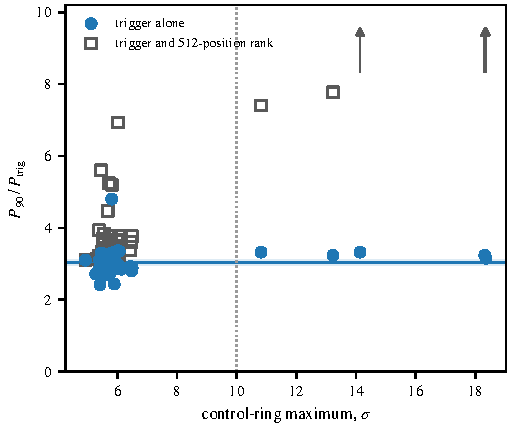
\includegraphics[width=\columnwidth]{figures/sens_ring.pdf}
%% ★ v4.26 (r25-captions): 9 printed lines -> R1 §7's limit of about six.
%% \S\ref{sec:pninetysel} above already carries every statement removed:
%% that the value does not depend on the ring's brightness, what charging
%% the rank would cost, and the bright-ring windows that cannot meet it at
%% any injected power -- the arrows.  \SensRingRule had this caption as its
%% only citation site, so the dotted line's threshold MOVED into that
%% paragraph rather than being dropped.
\caption{Why one completeness factor serves the whole class. The
\SensNInj{} directly injected Class~A windows at the power recovering nine
carriers in ten, each against its own \NCtrl-position ring maximum: no trend
with the ring. Filled, the criterion adopted here, pooled value as line and
band; open, the rank charged too, arrows where no power meets it; dotted, a
resolved ring.}
\label{fig:strata}
\end{figure}

\begin{figure*}
\centering
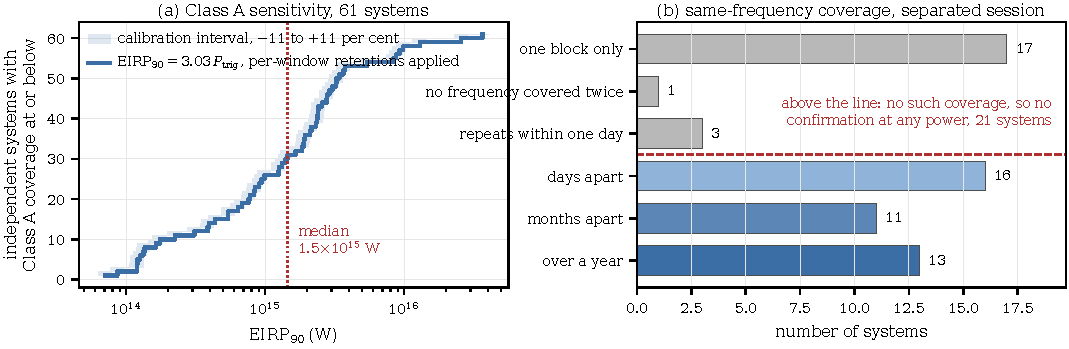
\includegraphics[width=\textwidth]{figures/classa_sensitivity.pdf}
%% ★ v4.26 (r25-captions): 9 printed lines -> R1 §7's limit of about six.
%% DELETED as said elsewhere and verified before deleting: "for an
%% accelerating carrier, confirmation further requires the repeat to fall at
%% a matching orbital phase" stands in Fig.~\ref{fig:confcov}'s caption AND in
%% \S\ref{sec:confirmability}; the grouping over "the primary census together
%% with every repeat block the recurrence test reads" is
%% \S\ref{sec:confirmability}'s own sentence; and the closing paragraph
%% re-states that section's opening line, "a sensitivity limit and a
%% confirmation limit are different statements", which is kept here in one
%% clause because it is what the figure is for.  No macro lost a site.
\caption{\textbf{The two completenesses of the carrier search, over the same
\NSysClassA{} systems}, which are separate statements and neither of which
follows from the other (\S\ref{sec:confirmability}).
\emph{(a)}~Single-epoch trigger completeness: the cumulative number of
systems whose best window reaches a given $\mathrm{EIRP}_{90}$, each
window's own retentions applied and atmospheric decorrelation excluded
(Table~\ref{tab:p90budget}, whose calibration interval is the shaded band).
\emph{(b)}~Systems with same-frequency coverage in a separated session,
which no amount of power buys, grouped by the longest separation between two
such sessions. \textbf{Left of the dashed line, \ZcNoRepSys{} systems have
no such pair, and for them confirmation was not possible at any sensitivity
in panel~(a)}.}
\label{fig:classasens}
\end{figure*}

\subsection{The nearest stars: Barnard's Star and Wolf~359}
\label{sec:barnardswolf}

Barnard's Star is the second-nearest stellar system and Wolf~359 the third if
brown dwarfs are excluded, and to our knowledge these are the first millimetre
or submillimetre technosignature limits for either; radio searches of
the nearest stars have worked at centimetre wavelengths \citep{Enriquez2017,
Price2020, Margot2023}. Both are non-detections. \emph{Both limits come from
the secondary Class~B experiment and not from the carrier search}: the archive
holds only coarse Band~6 windows toward these stars, so the
constraint is on an unresolved spectral excess and not on a
drifting carrier. On the $\mathrm{EIRP}_{90}$ convention of \S\ref{sec:pninetysel}
Barnard's Star reaches $\EirpNinetyBarnLo$--$\EirpNinetyBarnHi$\,W over
\NWinBarn{} windows. Wolf~359 reaches
$\EirpNinetyWolfLo$--$\EirpNinetyWolfHi$\,W over \NWinWolf.

\subsection{Threshold crossings and how each was disposed of}
\label{sec:technosearch}

\emph{The result is a chain of three tests, and it is read in one direction.}
Of the windows the search covers -- the \NWindows{} of the primary census
and the archival-tail blocks beside them -- \EvNCrossRaw{} hold a cell
reaching $T\geq5$ at the stellar position. \EvNCrossFlag{} lie in the one
execution block that fails the quality criterion of \S\ref{sec:bdblock}, which
was written after the condition was seen in that block and is insensitive to
where the line was drawn (Appendix~\ref{sec:blockquality}), so the population
that characterises the search is the \EvNCrossQp{} in quality-passing data and
those \EvNCrossFlag{} are reported beside it. The molecular-line mask is $\pm\MaskHalfKms$\,km\,s$^{-1}$ wide in each
star's own rest frame, and it places \MkNCoinc{} of the \EvNCrossQp{} within
that distance of a catalogued transition. A further \SoNCrossWord{} fall on
transitions of a species no debris disc has been shown to carry, which the
mask therefore does not hold; their offsets are reported and they stay
unattributed (Appendix~\ref{app:linemask}). That leaves
\EvNAttrQp{} crossings attributed and \EvNUnattrQp{} unattributed. The attributions are kinematic and not an accident of bandwidth: in the
frame the correlator delivered, the crossings with a measured peak frequency
crowd onto the transitions these setups were tuned to far more tightly than a
free landing on their own grids would put them (Appendix~\ref{app:rfi}). Of the unattributed,
\EvNRankQp{} outrank all \NCtrl{} control positions of their own window, and
none was found again in any other epoch covering its frequency. No
crossing survives the chain, and this survey reports no detection.
Figure~\ref{fig:chain} counts what survives each step and the crossing
ledger, which accompanies this paper as data, lists every crossing.

\emph{Anything bright in a window hides a weaker carrier behind it, so the
weaker cells were sought too.} The de-drifted statistic is retained in every
channel, so behind a window's tabulated crossing -- its largest cell --
weaker above-trigger cells can be read as well, neighbouring channels counting
as one: \CkNWin{} of the \NWinA{} Class~A windows retain such a profile and
hold \CkNSecondaryWord{} weaker cells, in \CkNSecWin{}
windows and as many as \CkNSecMax{} in one, of which \CkNSecAttr{}
are the resolved carbon monoxide of a disc spread over channels. The
\CkNSecUnattrWord{} unattributed ones, toward \CkSecStars, each have
\CkCovLo--\CkCovHi{} covering blocks, and \CkNRecurWord{} reaches the trigger
in any of them, the deepest repeat being $T_\star=\CkTrepHi$.
Cells are counted in the controls too, and outside the mask the star holds
slightly more of them than a control position at every level below the
trigger, with no step where a carrier search would put one; the displacement
is Appendix~\ref{app:falsealarm}'s and the expectation \S\ref{sec:trigunif}'s.

\subsubsection{The unattributed count is what the control positions predict}
\label{sec:trigunif}

The trigger is a threshold on a statistic and not a false-alarm rate: the
number of searched channel\,$\times$\,drift cells per window spans
\TuCellsDecades{} decades, so one level buys very unequal protection. How
many crossings chance should produce is therefore measured window by window,
over the \CeNWin{} Class~A windows of the census and with one condition on
both sides of the comparison: a cell at the stellar position that reaches the
trigger and that the line mask does not attribute. Both quantities are read from the data themselves, and
Appendix~\ref{app:falsealarm} gives that accounting. The control positions carry no continuum, so a calibration error varying
with frequency would raise the star and not them; on the continuum these
stars have, the least demanding window would need
\CyEpsMinPct{} per cent of it to reach the trigger, and the mild excess of
\S\ref{sec:technosearch} runs the wrong way with continuum brightness,
\CkRatioContBright{} against \CkRatioContFaint{} over the \CkNContWin{}
windows with a photospheric estimate (Appendix~\ref{app:radius}). These fields' own control positions predict \CeExp{} unattributed
Class~A crossings and \CeObs{} are found. A count that large or larger arises
by chance with probability \CeProbNull. Both sides are read over the whole
primary beam \S\ref{sec:statistic} defines. That is the primary reading, the
one the abstract and \S\ref{sec:summary} quote, and it is primary by
definition: it is the statistic Equation~\ref{eq:tstar} specifies, whereas a
narrower field drops the integrations whose pointing falls outside it and
with them on-source time and real signal. Read over such a field on both
sides the same comparison gives \FrNarrowObs{} against \FrNarrowExp{} at
$P=\FrNarrowProb$, reported here as a sensitivity test and not as a second
result. Both are extraction geometries applied uniformly to every window and
to both sides, so neither was defined by reference to the counts; neither was
nominated as the primary before the counts were compared, and with
\FrNRead{} readings tested the smaller probability corrected for \FrNRead{}
trials is \FrTwoTrialP, so neither reading departs from chance at the
\CeAlphaPct{} per cent level. The two disagree on \FrNFlag{} of the
\CeNWin{} windows and in both directions: the whole beam holds a crossing the
narrower field does not toward \FrUpStars, both of them attributed to carbon
monoxide, and the narrower field holds one the whole beam does not toward
\FrDownStars. The stars do carry more above-threshold cells than their own
controls below the trigger, and that excess has no identified cause; the rate
adopted is the control positions' own, and
Appendix~\ref{app:falsealarm} gives both readings and carries the excess
as a sensitivity test. A further \CeNTailCrossWord{} unattributed
crossings, both toward \CeTailStar, lie in archival-tail blocks the catalogue
does not tabulate window by window, and enter neither side.

That establishes consistency with the expectation these fields' own
control positions set, under the assumptions above, and not that the
unattributed crossings are noise: the most this comparison could not have
rejected is \CeAddLim{} further crossings against those same control
positions, \FrNarrowAddLim{} on the narrower reading. That is a statement of
compatibility under the model set out above -- one count per window, the
control positions' own rates, and the attribution applied to both sides --
and not an independently measured limit on a population of transmitters, nor
a confidence interval on one (Appendix~\ref{app:falsealarm}). Each
crossing is tested individually by the recurrence test of
\S\ref{sec:etacrv}.

\subsubsection{One execution block accounts for four of the crossings}
\label{sec:bdblock}

\BdNCross{} crossings belong to \BdStar{} (\BdAlias), all of them in one
ACA execution block, \texttt{\BdBlock}, whose whole field is above threshold.
\BdNCtrlAbove{} of its \BdNCtrl{} control positions exceed $T=5$, where the
median of a window's own control ensemble is \BdSurvCtrlMed{} across the
survey. Its single-integration noise is as predicted, \BdRmsMeas\,Jy against
\BdRmsPred\,Jy, but it does not integrate down. A jackknife on the channel
mean gives \BdJack\,Jy against \BdThermal\,Jy thermal, \BdJackRatio{} times
too large, while neighbouring channels stay uncorrelated (\BdChanCorr). The
two numbers describe a residual that persists from one integration to the next and differs from
channel to channel. Equation~\ref{eq:tstar} divides by the noise of the
stacked spectrum, which falls as the root of the integration count, so a
residual that does not average down accumulates along a drift track faster
than the denominator grows, and it does so at every position in the field; and
having no part common to the channels of one integration, it is not what the
continuum median of \S\ref{sec:statistic} removes. The \BdNSibling{}
sibling executions of the same field, array and setup reach only
$T_\star=\BdSibTMax{}$ and produce no crossing. \emph{The field is inflated and the star is not.} The strongest of the
four reaches $T_\star=\EvFlagTStarHi$ where its own controls peak at
\EvFlagCtrlAtHi, and \EvFlagNgeLo--\EvFlagNgeHi{} of the \BdNCtrl{} stand
above the star. The
criterion fails this block and no other, at any threshold between it and the
next most extreme block (Appendix~\ref{sec:blockquality}), so its
\BdNCross{} crossings are reported apart from the \EvNCrossQp{}; Appendix~\ref{app:rfi} carries what the block
might instead be. Milder cases of the same condition are not unique to it:
read window by window the same diagnostic flags \DqNWin{} windows in
\BkFlagNBlock{} blocks, and the \BkFlagNCrossOther{} flagged crossing outside
this block -- \BkFlagOtherStar{} -- is withheld for it too.

\subsubsection{Stellar flares are excluded by a broadband prediction}

Known flare stars are in the sample, but a millimetre flare raises every
channel of a window alike, so one able to produce a single-channel crossing at
the trigger must produce a $5\sqrt{N}\sigma$ continuum event in the same
integrations. Over the \FlNCont{} crossings with a recoverable continuum measurement
that prediction runs \FlPredLo--\FlPredHi$\sigma$. The observed continuum
statistic has median \FlObsMed, with $|Z|<3$ in \FlNQuiet{} of them. One block settles it: \FlEgStar{} \texttt{\FlEgEb} holds both a
crossing ($T_\star=\FlEgT$) and the millimetre flare of
\citet{MacGregor2020}, and that flare contributes \FlEgContrib$\sigma$
to the single-channel statistic -- raising the continuum at $Z=\FlEgContZ$
while the crossing's own de-drifted track reaches $Z_{\max}=\FlEgTrackZ$.

\subsection{$\beta$~Pictoris: an astrophysical positive control, and the
obstacle it identifies} \label{sec:bpicval}

\emph{A search that finds nothing must show that it could have found
something, and the survey's strongest features show exactly that.} The
pipeline recovers the $\beta$~Pictoris circumstellar carbon monoxide
without being told the disc is there: in two
rotational transitions and in \CsBpCoBlocks{} execution
blocks spanning \BpBaselineYr\,yr, drawn from \CsBpCoSess{}
observing sessions with each transition recovered in more than one of them,
the closest two being \CsBpCoSepMinD\,d apart.
In \NStageOneBpicEb{} of the blocks the star also outranks every control --
\BpicNFlagThree{} Band~3 windows at $T_\star$ up to \BpicBThreeTsym{} and
\BpicNFlagSix{} Band~6 windows at \BpicBSixTsym{} -- but the identification
is kinematic and does not rest on those
statistics: carried through the frame chain to the barycentre at each
block's own epoch and then to the star's rest frame, all \BpicPanelNCo{}
crossings lie within \BpicDvCoHi\,km\,s$^{-1}$ of the stellar systemic
velocity, in the two lowest CO transitions of a star with mapped
circumstellar CO \citep{Dent2014,Matra2017}, and the Band~3 peaks agree
across blocks to \BpRecThreeTuneChanMax{} channel once each block's own
tuning is removed. The alternative reading
requires a transmitter placed by coincidence at matched offsets from two CO
transitions of one star.

It is also the control that shows the recurrence test of
\S\ref{sec:etacrv} working in the positive direction: every flagged
$\beta$~Pictoris carbon-monoxide feature is recovered in another execution
block, and each transition in a block of another session as well, the
screened Band~6 window returning
$T_\star=\BpRecTTwo{}$ in the second block of its own recurrence set. A
non-recurrence elsewhere means nothing unless the same machinery recovers a
repeat where one exists.

\emph{One of those blocks is a counterexample, and it is the more useful half
of the control.} In it -- block \texttt{\BpCtrlBlock}, Band~\BpCtrlBand,
where the control ring reaches \BpCtrlRingMax{} against \BpCtrlStar{} at the
star -- several of the \NCtrl{} control positions exceed the
stellar statistic, so the spatial rank disfavours a window holding carbon
monoxide known to be real and centred on the star; the disc is resolved on
the scale of the primary beam in that configuration, which is the geometry
the statistic is built to reject. The rank is therefore a test of
compactness and not of authenticity, and on a real extended source it errs
conservatively -- a stronger statement than a clean positive control, because
it bounds the diagnostic's reach as well as demonstrating it
(Fig.~\ref{fig:bpiccontrol}).

%% fig:bpiccontrol MOVED to Appendix B (sections/app_C_spatialnorm.tex),
%% which is the appendix about the spatial statistic this figure bounds.
%% 0.36 pp off the main text; Sec. 5.4 cites it.


HD~48370 is the complementary case and is equally instructive. Its crossing
reaches $T_\star=\HdTsym$, but the control ring rises with the star, to
\HdRingMax, as emission filling the primary beam does. The velocity matches
the prominent CO($2{\to}1$) that \citet{Cataldi2023} report toward the
source and flag as possible cloud contamination. The block's
$^{13}$CO($2{\to}1$) window is bright at the ring and faint at the star.
The extended emission is therefore identified by the \emph{level} of the
control ring and not by the star's rank against it -- the star here outranks
every control -- which is why the window-level flag of
Appendix~\ref{sec:blockquality} is defined on the ring's median.

The mask that removes this emission covers \FrNSpec{} species and costs
\MkMaskAPct{} per cent of the Class~A union bandwidth, and it is nevertheless
the single most productive test in the chain
(Appendix~\ref{app:linemask}). \S\ref{sec:mmdifferent} draws the lesson.

\subsection{The two crossings that lead their own control fields}
\label{sec:vistest}

Frequencies in this section and the next are in the star's own rest frame,
which is the frame the recurrence test registers in; the delivered ones are in
Table~\ref{tab:cand} and in the ledger.

Two crossings reach a stellar statistic above every one of the \NCtrl{}
control positions in their own window, and neither is a detection. They are
\EvAStar{} at \RqFreqSx\,GHz and \EvBStar{} at \RqFreqCp\,GHz, both in
Band~\EvABand; both are tabulated in Table~\ref{tab:cand} and the first is
drawn in Fig.~\ref{fig:event}. At \EvAFlux$\pm$\EvAFluxErr\,mJy against
\EvARmsInt\,mJy per integration that first carrier is \EvAPerIntSig{}
standard deviations in any one of them and exists only in the drift-aligned
stack of all \EvADwellMin{} minutes on source, its fitted drift carrying it
\EvADriftChan{} channels of \EvAChanwkHz\,kHz across the block's
\EvAElapsedMin{} minutes of elapsed time. Their control rank is recorded because it says which crossing was examined
first, and it disposes of nothing (\S\ref{sec:method}).
\EvBStar's crossing lies $\EvBDv$\,km\,s$^{-1}$ from \EvBLine, a coincidence
reported as a note, not as a disposition
(Appendix~\ref{app:linemask}). Both events go on to the recurrence test. Each was also re-fitted in the visibility domain, as \LgNFit{} of the
\NCross{} crossings were, by phase rotating to the star and following the
recovered drift, and \LgNLocalCor{} of those fits are consistent with a point
source at the star. The fit excludes neither crossing: injected sources in
the bin these two occupy return
${\rm Re}/\sigma=\RsevReAtFiveMeanA\pm\RsevReAtFiveSdA$. Its value is that a pedestal fed through a sidelobe from elsewhere in
the field, which a dirty map at the star cannot tell from a source at the
phase centre, is not a point source there. Of the \NCtrl{} control positions
the rank screen uses, \RcNRetCtrl{} retain a dynamic spectrum and
\RcNVisCtrl{} are reachable in the visibilities.

Neither crossing is present when the same stellar-frame frequency is observed
again, and Table~\ref{tab:cand} gives both readings of that silence. The nearest covering block assumes least. It lies \RcSxNearH{} and
\EvBDeepH\,hours from each discovery, and rules out anything above
\RqNearFracSx{} and \RqNearFracCp{} of the discovery amplitude. Combining every covering block instead -- \RqNRepSx{} and \RqNRepCp{} of
them -- deepens that to \RcSxFive{} and \RcCpFive. It asks the same return
over baselines of \RqSpanDSx{} and \RqSpanDCp\,days, however, and not of
hours. Either
reading covers half a channel in the star's frame, $\pm\RqDispSx$ and
$\pm\RqDispCp$\,km\,s$^{-1}$, which each carrier's own fitted drift would
cross in \ZtSxLeaveSec{} and \ZtCpLeaveSec{} seconds: the
test asks for a return to that frequency, not a stability at
it (\S\ref{sec:etacrv}). Table~\ref{tab:cand} reports both readings as the
statistic a carrier persisting at the discovery amplitude $S$ would have
given at the predicted stellar-frame cell, $T_{\rm pers}$, against the
$T_{\rm rep}$ measured there with every repeat epoch combined by inverse
variance at the carried drift. That reading is one cell at one trial and so
may be negative, where each indented reading beneath it is a maximum and so
positive on average whatever is present. At the faintest amplitude consistent with each crossing
having been found at all, the criterion would have recovered a persisting
carrier with a calculated probability \RqPowerTrigSx{} and
\RqPowerTrigCp{}, and injected carriers at that amplitude are measured at
\HjMeasSx{} and \HjMeasCp{} in the accompanying data -- so for
\EvBStar{} the silence is not an exclusion and is not read as one. The same
chance computed at $S$ itself, which Table~\ref{tab:cand} gives in brackets,
is biased high.
Appendix~\ref{app:radius} follows its crossing through every step
of the chain.


\subsection{Recurrence, applied to every unattributed crossing}
\label{sec:etacrv}

A transmitter on a body in orbit about its star does not arrive at the same
frequency twice: its line-of-sight velocity changes between epochs, and a
carrier at a fixed rest frequency changes with it. The question the repeat
coverage can answer about such a carrier is therefore the broad one --
whether anything above the trigger is present again anywhere in a covering
window, searched at every drift of the grid -- and it is the result this
section leads with. That window is $\pm\WdHalfKms$\,km\,s$^{-1}$ wide in the
median case, against the $\pm\EcVexcKms$\,km\,s$^{-1}$ an orbit at the grid's
own \WdAGrid\,m\,s$^{-2}$ ceiling can produce about any star in this sample,
whatever its eccentricity and orientation, so it spans the excursion such a
carrier could have made. \WdNExc{} of the \WdNCov{} covering windows hold a
statistic above the trigger, and that is the number chance predicts in trials
of that size: \WdExpect. That expectation is a sum of each window's own
chance of holding one cell above the trigger, from its independent
channel--drift cells and the noise its own control positions measure, and
not a control rate applied to their number (Appendix~\ref{sec:pairacct}). The strongest of them reaches
\WdExcMax{} and the nearest sits \WdNearKms\,km\,s$^{-1}$ from the crossing's
own frequency, a median \WdMedKms\,km\,s$^{-1}$ away. A catalogued window
covers \WdNOrbTot{} of the \RcNExcl{} crossings that carry an exclusion and
spans that excursion in \EcNSpan{} of them; for \EcNShort, toward
\EcShortStarList, the widest covering window is narrower than the excursion,
and \WdNNoCov{} is covered by no catalogued window at all. Nothing recurs in
excess of chance.

Each of the \WdNExc{} repeat windows that hold something above the trigger
holds a crossing, so a carrier present again would appear in its repeat block
as one, and each pair must be asked whether one transmitter could have
produced both members. Inside that interval there are \TjNCandPair{} pairs in
which at least one member is unattributed
(Appendix~\ref{sec:pairacct} takes the one count to the other);
Table~\ref{tab:pairs} asks the question of the \TjNPair{} of them, across
\TjNStarPair{} stars, whose two crossings each carry an independently fitted
drift and a block epoch measured from their own data; \TjNCandLost{} cannot
be asked, for want of discovery products (\TjNCandLostSpec) or of a fitted
drift (\TjNCandLostFit). Both fitted drifts are
carried into the star's frame first, by removing the observatory's own
line-of-sight acceleration, which is diurnal here and so cannot be
extrapolated across days; Table~\ref{tab:pairs} marks that frame with the
subscript $\star$ and carries the stellar-frame offset $\Delta\nu$ beside the
two rates, while Appendix~\ref{sec:edge} gives the rates in the observatory's
frame, the frame the grid is stepped in. Constant line-of-sight acceleration means
$\dot\nu_1=\dot\nu_2$, which \TjNUneqDrift{} of the \TjNPair{} pairs fail by
more than the grid resolves, and the \TjNPower{} pairs whose rates the grid
resolves fail a drift changing at a constant rate as well
(Appendix~\ref{sec:pairacct}). The claim the measurement supports is
weaker and safer -- that no trajectory inside the searched grid joins the two
crossings -- and it separates \TjNExcl{} pair, the two crossings of
\EcGridStar{} needing \EcGridFactor{} times the grid's own ceiling between
them. Table~\ref{tab:pairs}'s \emph{Miss} column is that departure, measured
in units of the drift grid's own resolution over $\Delta t$, and a dash there
marks a pair the comparison has no power over at all.
The other \TjNOpen{} are unresolved, neither a confirmation nor an exclusion:
\TjNOpenPlain{} \emph{open} and \TjNPairEdge{} \emph{edge-limited}, where one
of the two fitted rates sits at the edge of the grid and is a lower bound and
which Table~\ref{tab:pairs} marks \emph{edge}. The comparison has the power to reject,
which it uses on all \TjNPower{} resolved pairs, and none to accept a drifting
carrier -- and it does accept the one pair that is a single emitter, the
\TjCtlLine{} line of \TjCtlStar, which is a line that does not drift and
which Table~\ref{tab:pairs} carries below its rule as a control row
(Appendix~\ref{sec:pairacct}).

The ledger's own exclusions answer a third and far narrower question: whether
a carrier returned to the single cell its own discovery predicts. That is a
test for a carrier whose stellar-frame frequency is unchanged between epochs
-- one at a fixed rest frequency, whose line-of-sight velocity relative to its
star is the same at the two epochs to within half a channel
(\RqHalfChanKHz\,kHz in the median case, $\pm\RqDvLo$ to $\pm\RqDvHi$\,km\,s$^{-1}$
across the \RcNExcl{} crossings that carry an exclusion, with a median of
$\pm\RqDvMed$), and which drifts through each observation at the rate fitted
there. The fitted drifts disfavour that model: every one of these crossings
carries a line-of-sight acceleration of \ZtALosLo{} to at least
\ZtALosHi\,m\,s$^{-2}$ in the observatory's frame, reaching \EgStarALosHi{} in
the star's own, which carries a carrier out of the half-channel the reading
covers in \ZtSxLeaveSec{} and \ZtCpLeaveSec{} seconds -- so a null result
there has little bearing on carriers of the kind these crossings would be, and
it is reported for what it is rather than as a result about persistence. The
same model is exactly right for an emitter at rest in the star's own frame,
which is what a spectral line is, and there the reading keeps its full force:
it is what recovers the line-attributed crossings below, and what any claimed
line identification for an unattributed crossing has to satisfy. A
\emph{confirmed signal} is an \emph{unattributed} crossing that satisfies the
criterion (Table~\ref{tab:quantities}); a line-coincident crossing that
satisfies it is a recurring molecular line, and is reported as one.
\RcNExclPoss{} of the \RcNTested{} unattributed crossings were read this way,
over \RcNRepeatMeas{} readings in \RcNRepeatBlock{} execution blocks -- the
test reads \ZcNRecEB{} blocks in all, those \RcNRepeatBlock{} together with
the \ZcNRecEBDisc{} discovery blocks that supply the other end of a
comparison and no repeat reading of their own -- at the
one channel the Earth's motion at the repeat epoch and the star's systemic
velocity predict, maximised over nothing, and none returned. The largest
statistic anywhere is $\RcTRepMax$ for a crossing's whole repeat coverage
combined at the \emph{carried drift} -- the rate fitted at the discovery epoch
and carried across to the repeat -- \RcTMatched{} read in one block alone at
that drift and \RcTMax{} at any drift of the grid, against a trigger of
\StageNullTrig. The amplitude such a reading reaches is the fraction of the
discovery amplitude still excluded at the trigger,
$(T_{\rm rep}+5)/T_{\rm pers}$: \RcNExcl{} crossings carry one,
\RcNWithheld{} take their discovery amplitude from the block that fails the
quality criterion of \S\ref{sec:bdblock} and \RcNNoSpec{} retains no discovery
spectrum. Over the \RcNExcl{} the repeat coverage rules out a carrier at a
median \RcFracMed{} of the discovery amplitude and \RcFracMin{} at best, and
\RcNFracBelow{} of the \RcNExcl{} rule out an amplitude below the discovery
amplitude at all -- but only just at the weak end, where the weakest rules out
\RcFracMax{} of it and \RcNFracWeak{} of them -- \RcFracWeakList{} -- rule out
nothing below \RcFracWeakLo. Each was measured as well as calculated, by
injecting a carrier at the trigger amplitude into the retained
per-integration spectra of every covering repeat block and reading it back by
the same procedure (Appendix~\ref{app:radius}):
\HjNPowerHi{} of the \RcNExcl{} reach \RcPowerLevel{} per cent recovery and
the other \HjNPowerLo{} -- \HjLowList{} -- are too shallow to test and are
reported as untested and not excluded. These are conditional detection
probabilities under the model this reading assumes, not probabilities that a
candidate was noise: a crossing that does not recur has not been shown to be
anything else. Neither the registration of that cell, nor the anchor along the
discovery track, nor the threshold itself changes any of these dispositions,
and Appendix~\ref{sec:regbudget} gives all three.

The reading works in the positive direction on real emission.
\MkAttrRecur{} of the \MkAttrTested{} crossings attributed to circumstellar or
interstellar carbon monoxide do recur, as expected, and they are the positive
control of this stage on both of the ways real emission arises here:
\RqNRecurDisc{} are the resolved circumstellar disc of \RqRecurDiscStars{} and
\RqNRecurCloud{} are interstellar gas toward \RqRecurCloudStars, whose
sightline carries catalogued cloud emission at the crossing's own velocity in
the local standard of rest (Appendix~\ref{app:linemask}). No exclusion is
formed for them, because what one would exclude has just been observed. The
control reaches across the baselines the exclusions are quoted over -- every
one of the \QcNCtl{} is recovered in a block more than \EpSep{} day from its
own and in a different observing session, \QcSepMinD{} to \QcSepMaxD{} days
away -- and close to the trigger it is thinner than
that count suggests: every circumstellar recovery has
$T_\star\ge\RqRecurDiscTLo$, and the \RqNearTrigN{} attributed crossings that
are not recovered are the two faintest tested, both at
$T_\star=\RqNearTrigT$, so there the stage is controlled by
\RqRecurCloudStars{} alone -- by interstellar gas and not by a point
source. What it establishes about the registration of a single cell rests on the
\RgRegNUnres{} readings of \RgRegStar{} alone, whose line is confined to one
channel; the rest test the frame correction only to the width of a resolved
line (Appendix~\ref{sec:regbudget}). The \MkAttrExcl{}
attributed crossings of the \MkAttrTested{} tested that are not recovered both
remain consistent with their attribution: each is bounded only \RqHrExcl{} and
\RqAjExcl{} standard deviations below what carbon monoxide persisting at the
discovery flux density would have given, and for the serendipitous field star
among them the attribution rests on a catalogued interstellar velocity and not
on this test (Appendix~\ref{app:linemask}).

\subsubsection{What can be searched, and what can be confirmed}
\label{sec:confirmability}

A sensitivity limit and a confirmation limit are different statements. This
experiment searched \RcSearchSys{} systems and \RcSearchWin{} Class~A windows
over \CvUnionA\,GHz of union bandwidth. Confirmation needs a second
observation of a frequency the first block covered, in another observing
session: \ZcConfSysDay{} of those systems have one more than a day later --
counting every block the recurrence test above reads and not the census alone
-- and \ZcConfSysYr{} of them more than a year later
(Fig.~\ref{fig:confcov}), while for the remaining \ZcNoRepSys{} no such block
exists and no transmitted power could have made a confirmation possible.
Requiring the different session as well as the day moves \QfNSysMovedWord{}
system, because each of the \QfNSysPairDropWord{} systems holding a
same-session pair more than a day apart holds a pair in two sessions as
well. Coverage is one limit on confirmation and
the criterion applied to the repeat is the other: a carrier accelerating as
these crossings do is back inside the interval a single cell permits for a
fraction of order $10^{\RgPhaseExpLo}$--$10^{\RgPhaseExpHi}$ of the phases of
an orbit at the searched ceiling, so for such a carrier a repeat at the same
frequency confirms nothing unless it also falls at a matching orbital
phase. What does bear on it is the window search and the pair test above, and
neither found a recurrence in excess of chance.

An independent execution block is also not an independent epoch. The baselines
run from \RcSepMinH\,hours to \RcSepMaxYr\,yr, and for \RcNSepSameDay{} of the
\RcNExclPoss{} crossings that carry a discovery amplitude at all the nearest
covering block falls within a day -- for \QcNHazard{} of those a block of the
same observing session as well, the two events of Table~\ref{tab:cand} among
them, whose nearest coverage lies \QcEvSepOneH{} and \QcEvSepTwoH\,hours
away. A recovery in a block of the discovery's own session would not have been
a confirmation. Read over blocks of another session more than a day away
alone, \SpNSep{} of the \RcNExcl{} keep such a block: \SpNExcl{} of those rule
out a carrier below the discovery amplitude, at a median \SpFracMed{} of it
and \SpFracMin{} at best, while \SpNVac{} rule out nothing at all, reaching
\SpFracMax. \SpNPower{} of them still reach \RcPowerLevel{} per cent recovery
at the trigger amplitude against \RqNPowerHi{} over every covering block;
both are modelled recoveries, comparable with each other and not with the
\HjNPowerHi{} the injections measure, which is the weaker reading and the one
quoted everywhere else here. The \QfNExclSameOnlyWord{} crossings
whose only coverage lies in their own session -- \SpNoSepList{} -- are all
among the \HjNPowerLo{} reported too shallow to exclude anything. Over months
and years these tests bound no duty cycle, and for the other \ZcNoRepSys{}
systems they bound nothing at all.
\subsubsection{The reserved hold-out and the control beyond 40\,pc}
\label{sec:holdoutsearch}

Three sets of execution blocks enter no census statistic
(Table~\ref{tab:blockledger}); each was searched with the same pipeline, each
holds data on real targets and each is reported here as a search. The hold-out is \HoNBlock{} blocks, \HoNWin{} windows, \HoNStar{} stars
and \HoHours\,h on source, set aside by the identifier rule of
Appendix~\ref{sec:heldout} and sharing no execution block
with the census. It contains \HoNCross{} threshold crossings,
the strongest at $T_\star=\HoTMax$, and none of them outranks its own
control positions: the fewest controls above the star in any of them is
\HoNCtrlMin{} of \NCtrl. \HoNTested{} were tested for recurrence on the same
code path as the census, and exactly one is present again -- \HoRecStar{} at
$\HoRecDv$\,km\,s$^{-1}$ from \HoRecLine, whose \HoRecNRep{} later blocks
combine to $T_{\rm rep}=\HoRecTRep$ at the carried drift. It is a molecular
line, so its recovery is the test working in the positive direction here as
well; for every other tested crossing the repeat coverage rules out a carrier
at \HoFracMax{} of the discovery amplitude or less. The hold-out crossings
are released row by row with the catalogue, on the columns of the crossing
ledger.

The archival extension was searched the same way. Its \LdgExtWin{} windows in
\LdgExtEB{} blocks hold \QxObsCross{} threshold crossings, every one in a
fine-channel window; \QxObsAttr{} lie inside the mask in their own star's
frame and \QxObsUnattr{} do not, against \QxLam{} predicted by chance over
the \QxNWinA{} fine-channel windows among them
(Appendix~\ref{app:falsealarm}), so the chance of \QxObsUnattr{} or more is
\QxPGe{} and the extension returns what the census's own fields predict. A
sample this size could have shown a shortfall and does not,
$P(0\,|\,\QxLam)=\QxPZero$. The frame these
offsets are read in is approximate -- no barycentric term is recorded for
these blocks, and \QxNVsysCross{} of the \QxObsCross{} carry a measured
systemic velocity -- but over the whole range either term can take the
unattributed count stays at \QxObsUnattrLo{} or \QxObsUnattrHi, and the
\ExtNStageOne{} crossings that outrank their own control positions are all
the $\beta$~Pictoris disc's carbon monoxide.

The control beyond 40\,pc is \OosNBlock{} blocks and \OosNWin{} windows
toward \OosNStar{} background sources, \OosHours\,h on source, holding
\OosNCross{} crossings, the strongest at $T_\star=\OosTMax$ and none of them
outranking its own controls. \OosVsysClause, so the set supports no limit and
shows only that the pipeline behaves the same way on fields beyond the
sample. The third reserved set calibrates the spatial rank
and is not external at all (Appendix~\ref{app:radius}).

\begin{figure*}
\centering
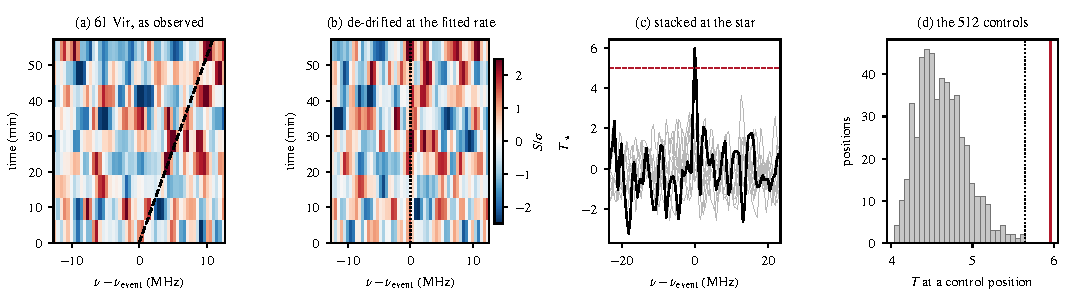
\includegraphics[width=\textwidth]{figures/event_crossings.pdf}
\caption{\textbf{The strongest unattributed crossing of the quality-passing
data, and the control field it leads.} Frequencies are in the star's rest
frame.
\emph{(a)}~The dynamic spectrum at \EvAStar's position around the crossing
at \RqFreqSx\,GHz, observed \EvADate, the fitted drift of
\EvADrift\,Hz\,s$^{-1}$ dashed, \EvANInt{} integrations binned into
\EvANBin{} and plotted in units of each bin's noise.
\emph{(b)}~The same rows shifted by that drift.
\emph{(c)}~The de-drifted stack at the star (black) and at the
\RcNRetCtrl{} control positions with retained dynamic spectra (grey), in
units of its own noise, the trigger dashed. \emph{(d)}~The same statistic at
each of the \NCtrl{} rank-screen control positions: the star (solid) against
the highest control (dotted).}
%% ★ v4.26 (r25-captions): 8 printed lines -> R1 §7's limit of about six.
%% MOVED into \S\ref{sec:vistest} above, carrying seven macros this caption
%% was the only citation site of (\EvAFlux, \EvAFluxErr, \EvARmsInt,
%% \EvAPerIntSig, \EvADwellMin, \EvADriftChan, \EvAChanwkHz,
%% \EvAElapsedMin): the per-integration significance and the drift's reach
%% across the block, both of which are statements about the crossing and not
%% keys to the panels.  DELETED: the closing pointer to
%% Table~\ref{tab:cand} and to \EvBStar{} at \RqFreqCp\,GHz, which
%% \S\ref{sec:vistest}'s own second paragraph states in the same words.
\label{fig:event}
\end{figure*}

\begin{table}
\centering
%% ★★★ v4.26 (r25-captions): 16 PRINTED LINES -> the author's limit.  Nothing
%% here was dropped on the floor: the $\pm\WdHalfKms$ interval and the
%% \TjNCandPair{} it holds are \S\ref{sec:etacrv}'s own second paragraph
%% already; \emph{edge} is defined there verbatim; and the subscript $\star$,
%% the observatory-frame pointer to Appendix~\ref{sec:edge} and the
%% \emph{Miss} column's units are now sentences in that same paragraph, which
%% is where a reader meets the table.  Measured with capmeasure.py.
\caption{\textbf{Can two crossings be one carrier?} The \TjNPair{} pairs
toward one star with an unattributed member. \emph{Miss}, the starred rates,
the control row and the verdicts: \S\ref{sec:etacrv}.}
\label{tab:pairs}
\scriptsize
%% GENERATED by pairs_v415.py -- do not hand-edit.
\begin{tabular}{@{}l@{~}l@{\hspace{4pt}}r@{\,}r@{\,}r@{\,}r@{\hspace{3.5pt}}r@{~}l@{}}
\hline
Star & blocks & $\Delta t$ & $\dot\nu_{1\star}$ & $\dot\nu_{2\star}$ & $\Delta\nu$ & miss & one \\
 & & (d) & \multicolumn{2}{c}{(Hz\,s$^{-1}$)} & (MHz) & ($\sigma$) & carrier? \\
\hline
61~Vir & X822/X82f & 3.00 & $+1092$ & $+3221$ & $+755.4$ & 15 & open \\
J1537$-$3319 & X10359/X398 & 123 & $-2000$ & $+2390$ & $+223.5$ & 3.6 & open \\
AU~Mic & X1838/X319 & 310 & $+1440$ & $+2645$ & $-159.0$ & -- & open \\
HD~14055 & X2b2ee/X2c3bb & 0.09 & $-2390$ & $+4216$ & $+825.2$ & 2447 & no \\
 & X24be0/Xd46 & 1.92 & $+1134$ & $-3823$ & $+63.0$ & 41 & open \\
 & X2c3bb/X3835 & 2.00 & $+4216$ & $+1800$ & $-514.6$ & 144 & edge \\
 & X2b2ee/X3835 & 2.09 & $-2390$ & $+1800$ & $+310.6$ & 48 & open \\
 & X3835/Xd526 & 607 & $+1800$ & $-2563$ & $-555.5$ & -- & open \\
 & X2b2ee/Xd526 & 609 & $-2390$ & $-2563$ & $-244.9$ & -- & open \\
 & X3835/X25c5e & 649 & $+1800$ & $+2611$ & $+423.3$ & -- & open \\
 & X2c3bb/X25c5e & 651 & $+4216$ & $+2611$ & $-91.3$ & -- & edge \\
 & X2b2ee/X25c5e & 651 & $-2390$ & $+2611$ & $+733.8$ & -- & open \\
$\beta$~Pic & X3a90/Xa9df & 1.02 & $-1611$ & $-679$ & $+85.5$ & 132 & open \\
\hline
HD~285968 & X108f/X5b4e & 4.99 & $-29$ & $-29$ & $-0.002$ & 0.6 & yes \\
\hline
\end{tabular}

\end{table}

\begin{table}
\centering
%% ★★★ v4.26 (r25-captions): 15 PRINTED LINES -> the author's limit.  The row
%% stubs of tab_recurcand_v411 already label $T_{\rm pers}$, $T_{\rm rep}$,
%% $(T_{\rm rep}+5)/T_{\rm pers}$ and the $\Phi$ rows in words, so the caption
%% was re-stating the table.  What was NOT anywhere else -- the sign of
%% $T_{\rm rep}$ against the indented maxima, and "in brackets the same at $S$,
%% which is biased high" -- is now \S\ref{sec:vistest}'s prose, two
%% paragraphs above this float.  The half-channel displacement is already in
%% that section ($\pm\RqDispSx$, $\pm\RqDispCp$) and the pointer to
%% Fig.~\ref{fig:event} is already in its first paragraph.
\caption{\textbf{The two events}, the crossings whose
stellar statistic exceeds all \NCtrl{} control positions of their own window.
\S\ref{sec:vistest} reads them.}
\label{tab:cand}
\footnotesize
%% GENERATED by recur_v411.py -- do not hand-edit.
\begin{tabular}{@{}>{\raggedright\arraybackslash}p{0.49\columnwidth}@{~~}r@{~~}r@{}}
\hline
 & 61 Vir & CP$-$72 2713 \\
\hline
Frequency, stellar frame (GHz) & 346.323236 & 344.296455 \\
\quad as delivered, topocentric & 346.313811 & 344.269746 \\
Drift rate (Hz\,s$^{-1}$) & $+3182$ & $-2056$ \\
$T_\star$ & 5.958 & 5.809 \\
Highest control $T$ & 5.65 & 5.68 \\
Fitted amplitude (mJy) & 118.8 $\pm$ 19.9 & 11.3 $\pm$ 2.0 \\
Peak-channel EIRP (W) & $5.1 \times 10^{14}$ & $8.9 \times 10^{14}$ \\
Repeat epochs measured & 3 & 5 \\
\quad of them in the primary census & 3 & 1 \\
\quad census repeats with no retained spectrum & 1 & 0 \\
Nearest covering epoch, separation (h) & $-1.97$ & $+2.05$ \\
\quad covering epochs more than a day away & 2 & 4 \\
Longest baseline (d) & 3 & 2 \\
$T$ expected if persistent, $T_{\rm pers}$ & 9.70 & 6.30 \\
$T$ measured, matched drift, $T_{\rm rep}$ & $+0.39$ & $-0.82$ \\
\quad largest single epoch & $+1.65$ & $+0.96$ \\
\quad maximised over every drift & 2.71 & 3.60 \\
Nearest block alone, $T_{\rm pers}$ & 5.28 & 6.21 \\
\quad $T_{\rm rep}$ & $-0.01$ & $-0.57$ \\
Amplitude still excluded, $(T_{\rm rep}+5)/T_{\rm pers}$ & 0.56 $S$ & 0.66 $S$ \\
\quad from the nearest block alone & 0.95 $S$ & 0.71 $S$ \\
\quad from separated blocks alone & \SpSxFracSep{} $S$ ($n=\SpSxNSep$) & \SpCpFracSep{} $S$ ($n=\SpCpNSep$) \\
\quad over the matched registration tolerance & \SpSxFracTol{} $S$ & \SpCpFracTol{} $S$ \\
Displacement permitted (km\,s$^{-1}$) & $\pm$0.211 & $\pm$0.213 \\
Calculated recovery chance $\Phi$ at $5S/T_\star$ (at $S$) & 1.00 (1.00) & 0.66 (0.90) \\
Disposition & not confirmed & not confirmed \\
\hline
\end{tabular}

\end{table}

%% ★★★★ TABLE 7 (tab:holdout) MOVED TO THE RELEASED FILES, round 25, to
%% the referees' guardrail "Table 7 may move to the catalogue".  It was a
%% full-width float of 0.20 pp carrying a 5-line full-width caption: 0.26 pp
%% in all, measured by floatinv.py and capmeasure.py.
%% ► ITS NAMED HOME, WHICH r25-zenodo MUST PROVIDE: the hold-out crossings as
%%   rows of the crossing ledger, carrying \Delta v_star (the offset from the
%%   nearest masked transition in the star's own frame), n_rep, T_pers, T_rep
%%   and the dagger flag for an offset inside the attribution interval whose
%%   species the attribution set excludes.  Sec. 5.6.2 carries the pointer.
%% ► NOTHING WAS DELETED FROM THE PROSE TO PAY FOR IT: the two readings the
%%   table carried that the text quoted, \HoRecTRep and \HoFracMax, are both
%%   still in Sec. 5.6.2; and the caveat its caption carried -- that a
%%   crossing inside the attribution interval whose species the set excludes
%%   is reported and not acted on -- is stated in Sec. 4.2 and Appendix C, so
%%   it survives exactly once, which is the referees' own rule.
%% ► To restore the float, revert this comment block; tab_holdout_v412.tex is
%%   still generated and still in make_all.sh.

%% tab:ledger MOVED to Appendix D (sections/app_J_falsealarm.tex): a
%% full-width 56-row table* worth 0.72 pp of the main text.  Sec. 5.3 and
%% Sec. 5.6 carry the counts and cite it.



%% fig:chain MOVED to sections/04_method.tex, Sec. 4.2, where it is first
%% cited (referee 2, minor 3).  Sec. 5 cites it at the crossing census.
%
\subsection{A stellar-frame multi-epoch stacked search}
\label{sec:stack}

Combining the epochs of a star in that star's own rest frame deepens the
limit. \EpMulti{} of the \NSystems{} surveyed systems hold more than one
searched execution block, and \SxStkStarCensus{} of the surveyed stars can be
stacked, \SttNStkOneEb{} of them from blocks beyond the census. Over
\SyStkNGroup{} stacked groups, \SyStkNEpochComb{} epoch-windows and
\SyStkHours\,h, the flux-density limit improves on each star's best single
epoch by a median factor \SyStkGainMed{} and by \SyStkGainMax{} at most;
\SxStkStarOutside{} further stars, all control stars beyond 40\,pc, stack too
and are excluded from those figures. Every
stacked limit is measured by injection into the stack itself and never read
off a stacked spectrum as a threshold.

\emph{A fixed stellar-frame frequency is not a fixed observed frequency, so
the epochs are registered before they are added.} The barycentric term alone
swings by a median \StkVcorrSwingMed\,km\,s$^{-1}$ between the epochs of one
star and by as much as \StkVcorrSwingMax{} -- many channels at the
\StkRefChanKHz\,kHz Class~A width -- so epochs added as observed would
dilute. Each epoch is transformed to the stellar rest frame,
divided by its own primary-beam response and combined by inverse variance
over the channels of common stellar-frame coverage, keyed on the star's
catalogued identity and not the directory the search ran in; spectra with
pathological archived visibility weights are excluded first
(\StkBadWeight{} of \StkNProd). The transform is verified on a real line:
over \StkRegNEpoch{} epochs spanning \StkRegSpanD\,d,
\StkPersistLineStar's molecular line collapses from a
\StkRegTopoChan-channel topocentric spread to \StkRegStellarChan{} channels.
The criterion is a stacked
$Z\ge\StkZmin$ above every stacked control maximum, no epoch supplying more
than \StkDomMax{} of the weighted sum, and at least \StkJkMin{} of the signal
surviving removal of the strongest epoch; controls are stacked identically
and every clause evaluated at them, measuring the whole test's
false-alarm rate at \StkCtrlFap{} per cent against a \StkFapCeil{} per cent
ceiling. \emph{The gain is $\sqrt{N_{\rm eff}}$ and not $\sqrt{N}$}, where
$N_{\rm eff}=\sigma_{\min}^{2}\sum_e\sigma_e^{-2}$ is the equivalent number of
equal-depth epochs and the median $N_{\rm eff}/N$ is \StkNeffFrac: against
$\sqrt{N}$ the realised gain is \StkGainVsN, the shortfall being unequal
epoch depth, so an epoch count alone misleads.

\emph{The deepest stacked limit is Proxima Centauri's, and it is a Class~B
limit.} Proxima is covered by \StkProxN{} blocks over \StkProxHours\,h
spanning \StkProxSpanYr\,yr, all of them coarse \ChanBModeMHz\,MHz windows,
so the stack constrains an unresolved spectral excess and discriminates no
drift. Stacking the census blocks alone, the set every other limit here uses,
gives $\mathrm{EIRP}_{90}=\SzProxEirpCensus$\,W; adding the rest of the
archive deepens that by \SzProxDeepen{} to $\StkProxEirpCal$\,W, against
$\StkProxEirpSingle$\,W for the best single epoch on the same convention.
The limit holds for an emitter steady in the stellar frame to within one
\ChanBModeMHz\,MHz channel, which is \StkProxTolKms\,km\,s$^{-1}$ peak to
peak, and \PxPlanet{} does not satisfy it. At \PxPorbD\,d about a star of
\PxMassMsun\,M$_\odot$ -- the archive's default parameter set
\citep{NEA2013}, for the planet of \citet{AngladaEscude2016} and a host mass
agreeing with \citet{Kervella2017} -- the planet moves at
\PxVorbKms\,km\,s$^{-1}$, so a
transmitter on it swings over \PxPPKms$\sin i$\,km\,s$^{-1}$, some
\PxNChanWalk{} channels at $\sin i=1$, and the stack cancels such a
carrier instead of building it unless the orbit is seen nearly face-on
($\sin i\le\PxSiniMax$, \PxIsoPct{} per cent of randomly oriented orbits).
Within a single block the same transmitter gains
at most \PxBlockDvKms\,km\,s$^{-1}$, \PxBlockPct{} per cent of one channel,
so the single-epoch limit of $\PxEirpSingle$\,W is the one that applies to
it -- \PxEirpRatio{} times shallower than the stack, and the deepest limit
this survey places on the nearest plausible transmitter site.

\emph{\StkNSurvive{} groups pass the full criterion and both are known
lines}: $\beta$~Pictoris carbon monoxide in two transitions, the astrophysical
positive control of \S\ref{sec:bpicval} passing in the stack as well. The
survey's own $\pm\StkAttrKms$\,km\,s$^{-1}$ mask leaves \StkUnattrClause.

Every stacked limit above holds only for a carrier that stays inside one
channel. At CO(2--1) one \StkRefChanKHz\,kHz channel spans
\StkTolFineKms\,km\,s$^{-1}$, the whole excursion a stacked carrier is
allowed, peak to peak, and a transmitter on a short-period giant planet whose
line-of-sight velocity swings by $\pm\StkReflexAmpKms$\,km\,s$^{-1}$ crosses
\SzReflexPPChanFine{} of those channels and de-registers completely, against
\SzReflexPPChanCoarse{} of a \ChanBModeMHz\,MHz window: the coarse stacks buy
reflex tolerance with bandwidth. Drift divides the same way, a
stack in \StkRefChanKHz\,kHz channels being confined to
\StkDriftTolHzS\,Hz\,s$^{-1}$ over the median inter-epoch span of
\StkSpanMedD\,d, and no crossing of \S\ref{sec:etacrv} drifts that slowly, so
toward the \SttNHostStar{} stars carrying them the stack is a deeper limit on
a non-drifting carrier and not a test of these events. Each
stacked limit therefore constrains only emitters stable in the stellar frame to
within its own channel; the single-epoch limits of \S\ref{sec:excludes} apply
generally.

%% ★ CUT HERE, round 25, to the referees' instruction "keep the method (one
%% paragraph) and Proxima (one paragraph); delete the HD 161868 example and
%% the beta Pic stacked-CO paragraph, which repeats Sec. 5.4".
%%
%% DELETED, with where each thing now lives:
%%  * the HD 161868 worst-stack example (\StkWorstStar, \StkWorstN,
%%    \StkWorstGain, \StkWorstNeff, \SzWorstSqrtNeff, \SzWorstNoise) -- an
%%    illustration of the sqrt(N_eff) point, which is KEPT as the point.
%%  * the realised-noise validation (\StkGainVsNeff, \StkMadZScatterPct,
%%    \SzNoiseLo, \SzNoiseHi): a validation result, so it is NOT simply gone --
%%    it belongs in the appendix with the rest of the stack validation, and is
%%    queued for the appendix owner rather than dropped.  The claim it
%%    supports ("the gain is sqrt(N_eff), not sqrt(N)") is weakened to exactly
%%    what survives: the measured ratio against sqrt(N), \StkGainVsN.
%%  * the beta Pic stacked-CO detail (\StkBpCoOne*/\StkBpCoTwo*,
%%    \StkBpCrossKms, \StkBpCrossChan, \BpicDvCoHi here) -- Sec. 5.4 carries the
%%    same control, and the RESULT (two groups pass, both known lines, none
%%    unattributed) is kept in full, because deleting a result is not a length
%%    saving.
%%  * HD 285968's own rejection by its controls (\StkPersistLineZ,
%%    \StkPersistLineCtrl).  The star itself stays: it is the registration
%%    standard, which is method.
%%  * Proxima's epoch provenance (\SxProxEbCensus, \SzProxEbSearched,
%%    \SzProxEbHold), its N_eff breakdown (\StkProxNeff, \SxProxSqrtNeff,
%%    \StkProxGain), \PxNEpoch/\PxFracSampled, \PxIncMaxDeg,
%%    \StkProxDriftHzS, \StkProxDistPc, \SttDriftMinHzS/\SttDriftMinMin,
%%    \SttNIncDisc.  The census-only figure \SzProxEirpCensus is KEPT and is
%%    named as the set every other limit uses, which is the one distinction a
%%    reader needs.
%%  * \StkLimitGainMed and \StkNStar: the all-stars median gain, which the
%%    census figures above already bound.
%%
%% NOTHING WEAKENED INTO A STRONGER CLAIM.  The two caveats in this subsection
%% -- that a stacked limit holds only for a carrier steady to within one
%% channel, and that the stack is not a test of the drifting crossings -- are
%% both KEPT, and the sqrt(N_eff) qualification is kept with the one number
%% that still supports it.
%%
%% ►► GATE CONSEQUENCES, all three handled in patches_cutmain.json:
%%  * \StkMadZScatterPct leaves valuetwin's seven-per-cent COINCIDENCE group
%%    (record G1);
%%  * \PxFracSampled's COINCIDENCE entry goes stale and is deleted (record G4);
%%  * \StkNStar leaves synmacro's nstar group (record G6), which is what
%%    exposed a defect in that gate's own note.
%%  * retire_macros --dry-run retires exactly FIVE macros across this whole
%%    pass -- StkBpCoOneN, StkBpCoOneOff, StkBpCoOneZ, StkBpCoTwoOff,
%%    StkBpCoTwoZ -- which are precisely the beta Pic stacked-CO detail the
%%    brief instructed be deleted, and no gate or generator names any of them.
%
\section{Discussion}
\label{sec:discussion}

\subsection{What is different about a millimetre technosignature search}
\label{sec:mmdifferent}

This experiment's most transferable result is not the non-detection but
a measurement of what limits a carrier search at these wavelengths. It is not
depth: the power a transmitter must radiate to cross the threshold here is a median
$\EirpNinetySysMedA$\,W per system, and more power buys nothing at a
frequency the archive never tuned to or never returned to. That
inherited coverage sets the limit. Molecular-line confusion is a different
matter: it costs bandwidth, and it decides how a crossing is disposed of once
one is found.

\emph{Line emission, and not interference, is the astrophysical false
positive here.}
Catalogued molecular transitions, almost all of them carbon monoxide, account
for \EvNAttrQp{} of the \EvNCrossQp{} crossings in quality-passing data, and
no crossing in this survey is attributed to interference
(Appendix~\ref{app:rfi}). \LnAttrSupp{} of those attributions carry support
beyond the frequency match -- a second transition of the same species,
catalogued gas on the sightline, or the crossing's own recurrence -- while
\LnAttrCoincWord{} rest on the coincidence alone, which leaves them
consistent with molecular emission and not identified as it. The
attributed crossings include the strongest events in the quality-passing
data, but they are
not the commonest: of the \EvNUnattrQp{} unattributed crossings the \CeObs{}
of the primary census are no more numerous than the control positions of
their own fields predict
(\S\ref{sec:trigunif}), so chance at a trigger of \StageNullTrig{} is enough
to account for most crossings by number while line emission accounts for the
ones that stand out.
\DiscFpWin{} of the \DiscFpOfFlags{} windows that reached the spatial stage
are disc or interstellar carbon monoxide, all but one the resolved disc of
$\beta$~Pictoris and the exception a cloud along the sightline to
HD~48370. The remedy that works is a velocity-space mask evaluated in each star's
own rest frame, and \S\ref{sec:bpicval} gives what it costs in
bandwidth.

\emph{Spatially extended emission is the second discriminant, and it has no
analogue at centimetre wavelengths.} A line filling the primary beam raises
the star and the control annulus together instead of cancelling, so the
spatial statistic loses power exactly where circumstellar gas is brightest:
$\beta$~Pictoris shows the benign face, its circumstellar carbon monoxide
recovered by the same search (\S\ref{sec:bpicval}), and HD~48370 the other,
its emission an interstellar cloud and not a disc
(Appendix~\ref{app:linemask}), lying near a band edge, and that one window
contributing \VnEdgeDomPct{} per cent of every near-edge threshold exceedance
in the survey. Pooled, the near-edge rate is $\times\VnEdgeRatio$ the
interior rate; without that window it is $\times\VnEdgeNoDomRatio$, and on a
held-out half $\times\VnEdgeHalfCleanRatio$
($\pv{\VnEdgeHalfCleanP}$). That near-edge excess is
one interstellar cloud, so no edge correction is
applied to any limit.

An illustrative engineering benchmark fixes the scale these limits reach. A
\BenchDiam\,m dish radiating \BenchPowerMW\,MW at \BenchFreqGHz\,GHz with an
aperture efficiency of \BenchEta{} has a directive gain
$G=\eta(\pi D\nu/c)^{2}=\BenchGain$ and so an EIRP of $\BenchEirp$\,W, above
the single-epoch crossing limit of \BenchNSysA{} of the \NSysClassA{} Class~A
systems. The same gain makes its beam $\Omega=4\pi/G=\BmOmegaSr$\,sr,
illuminating $\BmSkyFrac$ of the sky with a half-power width of \BmArcsec{}
arcsec, and EIRP is not transmitter power -- the same megawatt radiated
isotropically would be $10^{6}$\,W -- so these limits apply to beamed
transmitters whose beam contains the Solar System.

\emph{The channelisation is inherited.} In \ScCoarseNoDrift{} of the
\NWinB{} coarse-channel windows every drift in the grid stays inside one channel over a
whole track and in \EtaDriftBHi{} more it crosses barely one; none of them
can distinguish a drifting carrier from a stationary one, which is why the
carrier search rests on the \NWinA{} fine-channel windows. The widths on offer here run from \SzChanFinestKHz\,kHz to
\SzChanWidestMHz\,MHz, about \SzChanDexSurvey{} orders of magnitude. Set
beside the \SzChanLitHz\,Hz channels of centimetre-band carrier searches the
range becomes \SzChanDexAll{} orders (Fig.~\ref{fig:context}(b)), and
nothing in the search could choose them.

\emph{Repeat epochs turn a crossing into a testable claim, and an archive
supplies them only incidentally.} Let the \emph{confirmation coverage}
$C_{\rm conf}(\nu)$ be the number of systems toward which two execution
blocks of different observing sessions more than a day apart both cover the
sky frequency $\nu$, so
that a carrier found once there could have been sought again. It must be
stated against frequency and not as a fraction of the sample, because
repeat visits re-tune and a second epoch is of no use at a frequency it does
not cover. Its support is \CvConfGHzDay\,GHz of union bandwidth, \CvConfPctDay{} per
cent of the \CvUnionA\,GHz searched, and it falls to \CvConfGHzYr\,GHz
beyond a year. At its best, near \CvConfNuMaxDay\,GHz, it reaches
\CvConfNMaxDay{} systems (Fig.~\ref{fig:confcov}). The searched extent
is about twice the extent over which a carrier returning to its predicted
cell could have been
confirmed, and for close to half the sample the archive constrains an
intermittent emitter hardly at all, whatever its power.

\begin{figure}
\centering
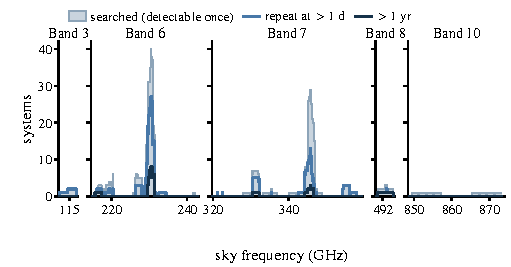
\includegraphics[width=\columnwidth]{figures/confcoverage.pdf}
%% ★ v4.26 (r25-captions): 8 printed lines -> R1 §7's limit of about six.
%% "a block of another observing session more than a day later" IS the defined
%% term \emph{separated} (Table~\ref{tab:quantities}), so naming the term is
%% both shorter and the paper's own usage.  The orbital-phase caveat is KEPT
%% here: it was dropped from Fig.~\ref{fig:classasens}'s caption, which
%% carried it as well, and this is the panel it bites hardest on.  "as in
%% Fig.~\ref{fig:covmap}" went because that caption states the same panel
%% rule in the same words.  No macro lost a citation site.
\caption{What could be searched against where a separated repeat exists.
Class~A systems against sky frequency: detectable once (grey); with a
\emph{separated} block (Table~\ref{tab:quantities}) covering it (blue);
beyond a year (dark). An accelerating carrier further needs a matching
orbital phase. One panel per populated ALMA band, width proportional to its
frequency share.}
\label{fig:confcov}
\end{figure}

\subsection{The search space this archive opens}
\label{sec:newspace}

The searches of \citet{Steffes1994} and \citet{Mauersberger1996} reached
nearby stars above about 30\,GHz at one frequency only, and the one other
millimetre search of more than a single line, \citet{Mason2025},
covered \MasonBandMHz\,MHz of Band~3 toward far more distant stars
(\S\ref{sec:intro}); Band~3 is searched here, in
\NWinBandThree{} windows down to \SurvFreqLo\,GHz including
$\beta$~Pictoris' CO $J=1\!-\!0$ control. The haystack axis of \citet{Wright2018} runs from \SttHayLoMHz\,MHz to
\SttHayHiGHz\,GHz, and this experiment covers \SttHayGHz\,GHz of it. Only
\SttHayFineGHz\,GHz of that is carrier search, because the Class~A union
spans \SurvFreqLoA--\SurvFreqHiA\,GHz, and the rest lies above the axis
altogether.

Union bandwidth overstates what that buys: different frequencies were searched
toward different numbers of stars and to very different
limits. Figure~\ref{fig:covmap} gives instead the number of independent systems
that would have yielded a recovery at ninety per cent completeness, against sky
frequency and transmitter power. At an EIRP of $\CovEirpRefTex$\,W the covered frequency falls to
\CovUnionAtRef\,GHz, which is \CovFracAtRef{} per cent of the union. It
reaches \CovNSysAtRef{} systems, and \CovNMaxAtRef{} at the best-covered
frequency near \CovNuMaxAtRef\,GHz. With no limit on power at all that
frequency reaches \CovNMaxFull{} of the \NSysClassA{} systems, and half the
sample is reached only above $\CovEirpHalf$\,W.

\begin{figure}
\centering
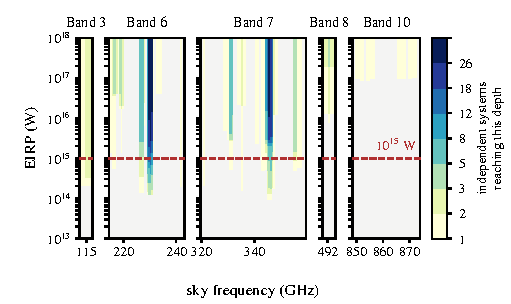
\includegraphics[width=\columnwidth]{figures/completeness_map.pdf}
%% ★ v4.26 (r25-captions): 10 printed lines -> R1 §7's limit of about six.
%% DELETED after checking each: "that is a recovery completeness" restates the
%% clause before it; and "the Class~A union being \CovNIslands{} disjoint
%% islands across \DomAFreqLo--\DomAFreqHi\,GHz" is \S\ref{sec:coverage}'s own
%% sentence, and the abstract's and Conclusion 1's -- all three macros keep
%% two or more citation sites, checked before deleting.
\caption{Where the experiment could have found something. Shading, the
independent systems recovering an unresolved carrier of the plotted EIRP and
sky frequency nine times in ten \emph{in a single epoch}; unshaded, none.
Confirmation needs a second epoch covering the same cell, which no power
supplies. Panels as in Fig.~\ref{fig:confcov}, which gives that coverage.
Dashed, $\CovEirpRefTex$\,W.}
\label{fig:covmap}
\end{figure}

On the continuous-waveform transmitter figure of merit of
\citet{Enriquez2017}, with the single survey-wide fractional bandwidth
replaced by the star-bandwidth product an archive requires, this experiment
is $\CwBareMed$ on the median system and $\CwBareWorst$ on the sample's
largest threshold power.\footnote{The denominator is the star-bandwidth
product $\sum_{i}\Delta\nu_{i}/\nu_{i}$, one term per system, in which
$\Delta\nu_{i}$ is the union of that system's own searched windows and
$\nu_{i}$ the midpoint of the span they cover: \CwSigma{} over the
\CwNSys{} systems against \CwUniform{} on a single survey-wide fractional
bandwidth, a factor \CwRatio{} apart because the median system was covered
over only \SysUnionAMed\,GHz of the \CvUnionA\,GHz union. An archive
searches different frequencies toward different stars, which a single
fractional bandwidth credits to every system alike. The published values are
read at the common threshold of Table~\ref{tab:litthresh}, where
\FomLitEnriquez{} becomes \FomLitEnriquezFive{} and \FgLitMargot{} becomes
\FgLitMargotFive; \citet{Margot2023} publish no figure of merit, and the
value quoted here is the same expression on the \FomMargotN{} stars,
\FomMargotLo--\FomMargotHi\,GHz and $\mathrm{EIRP}>\FgMargotEirp$\,W
they do give.} That is a factor $\CwRatioEnriquezFive$ above the
Enriquez value once both are read at the same threshold, which splits into
\CwBandDex{} decades of haystack and \CwEirpDex{} decades of depth: a far
smaller haystack than a wideband centimetre survey of thousands of stars,
and a shallower one.

\subsection{What this experiment excludes, and what it does not}
\label{sec:excludes}

\noindent\emph{The signal these limits describe.} Every limit here applies to
one kind of signal: an unresolved carrier at the stellar position, confined to
a single \ChanLoA--\ChanHiA\,kHz channel, lying outside the molecular-line
mask, radiating while one of the archival blocks is on sky, and changing
frequency linearly at no more than its own window's ceiling,
\DriftCeilLo--\DriftCeilHi\,nHz. Such a carrier would
have produced a crossing nine times in ten above the nominal
$\mathrm{EIRP}_{90}$ of \S\ref{sec:pninetysel}, which leaves out
atmospheric decorrelation, and none survived toward any of the \NSysClassA{}
systems the carrier search covers. Four conditions
bound it as sharply as power does: the coverage is sparse and
inherited (Fig.~\ref{fig:covmap}); the drift grid reaches an acceleration that contains every
known planet of the sample but one, while a transmitter on a rapidly rotating
planet spends most of that reach on its spin alone (Fig.~\ref{fig:accel}); emission broader than one channel is
retained but unmatched by the single-channel filter, which needs close to
\ScNBroadRatio$\times$ the total power for a feature as wide as the widest line these
fields show, so the thresholds quoted here do not apply to it; and a carrier on for part of a block comes
back at that fraction of its amplitude, while one absent throughout is not
constrained at all.

\noindent\emph{The result is a non-detection and not an exclusion of
persistent transmitters.} Recurrence applies over a far smaller domain than
the limits do: where the archive observed a frequency only once no
transmitted power makes a confirmation possible
(\S\ref{sec:confirmability}), and where the test does apply it has power
only against a carrier as strong as the trigger demands of the repeat, so a
shallow repeat excludes nothing. Three propositions then have to be kept
apart. A
transmitter radiating continuously at a fixed intrinsic frequency is not
tested here at all, because its observed frequency follows its own
line-of-sight velocity. A return to the same observed stellar-frame frequency
is what the reading at a single cell tests, and it is not found. Remaining
above the detection threshold at both epochs is a third condition, and
\HjNPowerLo{} of the \RcNExcl{} crossings that carry an exclusion fail
it. Four further restrictions on that reading are ours. A transmitter
operating intermittently need not have been radiating during the second
block. A second block need not cover the frequency at all, and over about
half the searched bandwidth none does (\S\ref{sec:mmdifferent}). A
transmitter accelerating as these crossings do crosses the half-channel the
cell permits in seconds, so it is back inside it only at a matching orbital
phase, and what bears on such a carrier is the search over the whole covering
window and the pair comparison of \S\ref{sec:etacrv} -- a population
statement, not an exclusion of any one of them. And a transmitter may change
frequency deliberately, which nothing here addresses. Outside the adopted criterion, then, nothing
is excluded: neither emission inside the
$\pm\MaskHalfKms$\,km\,s$^{-1}$ molecular-line mask at any strength, nor any
emission from the stars within 40\,pc that ALMA has not
observed, which is almost all of the \NGaiaCensus{} this volume holds.

\noindent\emph{Two blind spots.}
$(\mathrm{XX}+\mathrm{YY})/2$, which retains the full intensity of a circularly polarised
carrier; the loss is not sensitivity but the discrimination
polarisation would offer against unpolarised astrophysical emission, because ALMA's feeds
are linear and the circularity lies in the cross-hands, which this analysis
does not extract. And the frequency coverage is the archive's and not a
choice: the \SbPriorFreqGHz\,GHz positronium hyperfine line that
\citet{Steffes1994} and \citet{Mauersberger1996} observed lies in ALMA Band~5,
where this survey holds
\LnBFiveWin{} coarse-channel windows, all toward \LnBFiveStars, and none of
them covers it.

\subsection{What a dedicated ALMA technosignature experiment should do
differently}
\label{sec:future}

A purpose-built experiment on the same telescope would be far stronger, and
the changes it needs follow from the limitations above.

\begin{itemize}[leftmargin=1.2em,itemsep=2pt,topsep=3pt,parsep=0pt]
\item \emph{Channelise finely everywhere.} The \NCoarse{} coarse-channel
windows cannot carry a carrier search at all.
\item \emph{Choose the targets and the frequencies.} An archive weighted
toward dusty discs is the worst case for molecular-line confusion, the
M~dwarfs that dominate the nearby habitable-zone planet census are the least
covered, and windows placed deliberately away from the bright transitions
would recover most of the \MkMaskAGHz\,GHz of the \CvUnionA\,GHz Class~A
union that the mask costs.
\item \emph{Repeat the epochs on purpose, at the same tuning.} Two or three
visits separated by days and by years turn a crossing into a testable claim,
and the separation is a scheduling constraint rather than extra sensitivity
(Fig.~\ref{fig:confcov}). Two epochs cannot test an orbit, only fit one;
three separated epochs over-determine it, and \PaNSysThree{} of the
\NSysClassA{} systems here already carry three at a common frequency, so the
shortfall is not coverage but a candidate seen at more than one of them.
\item \emph{Retain the visibilities.} Rotating the phase centre to the star
leaves a genuine point source entirely in the real part of the visibility,
which asks whether the data contain a source where the star is -- a stronger
question than any rank against neighbouring positions in an image.
\end{itemize}
%
\section{Conclusions}
\label{sec:conclusions}

\begin{enumerate}[leftmargin=1.6em,itemsep=4pt,topsep=4pt,parsep=0pt]

\item \emph{What is new, and what was searched.} In the millimetre band the
record for nearby stars is two measurements of one spectral line:
\citet{Steffes1994} and \citet{Mauersberger1996} each covered no more than
\SbPriorBandMHz\,MHz at narrowband resolution around the
\SbPriorFreqGHz\,GHz positronium line, with no search over drift rate and no
epoch-to-epoch test of persistence. The carrier search here is \NWinA{}
fine-channel windows toward \NSysClassA{} systems within 40\,pc, covering
\CvUnionA\,GHz of unique frequency in \CovNIslands{} disjoint intervals --
at least \SbPriorRatio{} times that bandwidth -- of which \EdrNWinA{} windows
carry a track long enough for the searched drift to cross a channel,
\EdrUnionGHz\,GHz toward \EdrNSys{} systems. A coarse-channel search for a
steady unresolved excess adds \NWinB{} windows toward \PrSysClassB{} systems,
both from one pass through \NEB{} public ALMA execution blocks spanning
\SurvFreqLo--\SurvFreqHi\,GHz (\S\ref{sec:sample}).

\item \emph{How deep.} The median system's best window would have produced a
threshold crossing from a carrier of $\EirpNinetySysMedA$\,W nine times in
ten, and \NSysEfifteen{} systems reach $10^{15}$\,W on that measure;
combining each star's epochs in its own rest frame deepens the flux-density
limit by a median factor \SyStkGainMed, the deepest being Proxima Centauri's
$\StkProxEirpCal$\,W in coarse \ChanBModeMHz\,MHz channels, which bounds a
steady unresolved excess and not a drifting carrier (\S\ref{sec:stack}).
That is the completeness of a single observation and not of a confirmation
(\S\ref{sec:confirmability}), and for \SmcNEstSys{} of the \NSysClassA{}
systems it is carried across from the windows injected into rather than
measured in their own. It also leaves out atmospheric decorrelation, which a
real carrier suffers and an injected one does not, so the net bias on any one
limit runs either way and Table~\ref{tab:persys} gives it system by system
(\S\ref{sec:pninetysel}).

\item \emph{What was found.} The search produced \EvNCrossRaw{} threshold
crossings -- \CkNCrossCenA{} Class~A in the primary census,
\CeNTailCrossWord{} Class~A in archival-tail blocks that enter no
expectation, and \PrFlagXrossWord{} Class~B which all come from the single
execution block that fails the data-quality criterion of
Appendix~\ref{sec:blockquality} -- so the quality-passing data hold
\EvNCrossQp{} crossings, every one of them from the carrier search.
\EvNAttrQp{} of those are attributed to a catalogued molecular transition
within $\pm\MaskHalfKms$\,km\,s$^{-1}$ of the star's velocity, circumstellar
or interstellar, and \EvNUnattrQp{} are not; an attribution is not an
identification, and \S\ref{sec:mmdifferent} says which of them carry evidence
beyond the coincidence. Of the unattributed, \CeTlObsCutWord{} is
atmospheric, leaving \CeObs{} of the primary census to set against the
\CeExp{} these fields' own control positions predict at
probability \CeProbNull{} -- consistency, and not a demonstration that the
crossings are noise, since a further \CeAddLim{} would have been consistent
too (\S\ref{sec:technosearch}, \S\ref{sec:trigunif}).

\item \emph{What the repeat observations show, and what could have been
confirmed at all.} Nothing came back. A transmitter on an orbiting body
arrives at a frequency its own motion has moved, so the test that bears on
one is the broad one, and every unattributed crossing another block covers
was searched twice over that way: across the whole covering window at every
drift of the grid, where \WdNExc{} of the \WdNCov{} windows hold a statistic
above the trigger against the \WdExpect{} chance predicts in trials of that
size; and pair by pair, where of the \TjNPair{} pairs of crossings carrying
enough measurement to be asked the searched grid separates \TjNExcl{} and
leaves \TjNOpen{} unresolved, \TjNOpenPlain{} \emph{open} and
\TjNPairEdge{} \emph{edge-limited}. Neither finds a recurrence in excess of
chance. Nothing returned to the single cell a crossing's own discovery
predicts either, the largest statistic anywhere being \RcTMatched{} at the
drift fitted at discovery and \RcTMax{} at any drift of the grid, against a
trigger of \StageNullTrig; the same reading recovers \MkAttrRecur{} of the
\MkAttrTested{} line-attributed crossings it was tested on, each in a
different observing session more than a day away, so the machinery does
return a repeat where one exists. What that reading tests is narrow, and the
narrowness belongs to the criterion and not to the archive: it requires a
carrier radiating in both observations whose stellar-frame frequency comes
back to within half a native channel, and a transmitter accelerating at the
\ZtALosLo{} to \ZtALosHi\,m\,s$^{-2}$ these crossings themselves show
re-enters that interval only if its motion is periodic and the second epoch
catches it at the matching phase, so this is not a test of a persistent
transmitter of any kind. Of the \NSysClassA{} systems covered,
\ZcConfSysDay{} were observed again in another observing session more than a
day later at a frequency the first block covered and \ZcConfSysYr{} more than
a year later, while for the remaining \ZcNoRepSys{} no repeat exists, so no
transmitted power would have made a confirmation possible: coverage is one
limit on confirmation and the criterion applied to the repeat is the other
(\S\ref{sec:confirmability}, \S\ref{sec:etacrv}).

\item \emph{What this does not constrain, and what would change the answer.}
These limits hold only inside the domain actually searched: the drift grid
stops at \DriftCeilLo\,nHz, \AccelSheikhPct{} per cent of the ceiling
recommended for a general carrier search \citep{Sheikh2019}, so an unbound
transmitter, one on a rapidly rotating planet, or one whose orbital and
rotational accelerations together exceed that is not constrained here at all
(\S\ref{sec:excludes}). The obstacle transfers beyond this archive:
channelisation chosen by other observers, and not collecting area, decides
which search is possible. Three choices a proposal can simply make would lift
it -- fine channels everywhere, frequencies and targets chosen against the
line forest rather than inherited from programmes that sought it, and repeat
visits at one tuning days and years apart (\S\ref{sec:future}).

\end{enumerate}

%% ★★★★ ROUND 25: EIGHT NUMBERED CONCLUSIONS BECAME FIVE, to R1's "no more
%% than five short paragraphs".  Merged: old 1+2 (what is new / what was
%% searched) into 1; old 7 (stacking) into 2, keeping the median gain and
%% Proxima's deepest figure and dropping the inclination arithmetic, which
%% Sec. 5.7 carries; old 5+6 (repeat exclusions / confirmability) into 4.
%% Item 4 runs to six sentences rather than three: it carries two merged
%% items and A1's reframing, and R1's binding constraint is the FIVE
%% paragraphs, not a sentence count.
%%
%% ★★★★ THIS FILE FOLDS IN TWO OTHER AGENTS' HUNKS, because a whole-file
%% record would otherwise clobber them and their own `old` strings are
%% anchored in the PRISTINE eight-item structure that no longer exists:
%%  * r25-recur (recur.patch, both hunks on this file): A1's reframing.  The
%%    broad window search and the PAIR TEST become the headline recurrence
%%    result and the single-cell reading is demoted to "Nothing returned ...
%%    either"; the item is retitled "What the repeat observations SHOW" and
%%    not "exclude"; \TjNOpenPlain and \TjNPairEdge are theirs; and old item
%%    6's close becomes "coverage is one limit on confirmation and the
%%    criterion applied to the repeat is the other".
%%  * r25-cut-app (patches_cutapp.json X3.1): "(Table~\ref{tab:confirm})" is
%%    removed, Table D3 having moved to the deposit.
%% ►► IF r25-recur REVISES ITS TEXT AFTER THIS RECORD WAS WRITTEN, THIS FOLD
%%    IS STALE AND THEIRS WINS -- re-read before integrating.
%%
%% ★★★ RULING 11.2 RE-POINTS censusacct_r17's A4 AT SEC. 5.3, AND I HAVE
%% DELIBERATELY NOT TAKEN THE LICENCE IT OFFERS.  A4 required THIS file to
%% carry \CkNCrossCenA, \PrFlagXrossWord, "\CeNTailCrossWord{} Class~A",
%% \EvNCrossRaw and \EvNCrossQp, and the sentence carrying \PrFlagXrossWord
%% also to say "fails the data-quality criterion" and name a "single execution
%% block".  Item 3 above still satisfies A4 in ONE sentence instead of four,
%% for two reasons that are measurements and not caution:
%%  (1) \PrFlagXrossWord is cited in exactly TWO files, this one and
%%      sections/abstract.tex.  r25-abs is rewriting the abstract to 180-200
%%      words; if that drops it and this file drops it too, retire_macros
%%      deletes the macro and the flagged-block count leaves the paper
%%      silently.  Keeping it here costs one clause and removes that coupling.
%%  (2) The record therefore applies whether or not the A4 re-point has landed
%%      in the integration tree, which a record that is the only surviving
%%      copy of the work ought to do.
%% ► A fuller cut IS available and is the integrator's to take: delete the
%%   dash-clause naming the three sets from item 3 once (a) the A4 re-point is
%%   in the tree and (b) \PrFlagXrossWord is confirmed still cited elsewhere.
%%
%% ★★ WHAT WENT, AND WHERE IT LIVES.  The narrower-field reading
%% (\FrNarrowObs, \FrNarrowExp, \FrNarrowProb, \FrNarrowAddLim) is no longer
%% quoted here: the coordinator's A2 ruling puts the alternative reading in
%% Sec. 5.3.1 and Appendix D as a labelled sensitivity test, and B9 asks for it
%% to be quoted ONCE.  The primary reading kept here is the one that is NOT
%% significant, so dropping the alternative cannot strengthen a claim.
%% Proxima's inclination condition (\PxNChanWalk, \PxIncMaxDeg,
%% \PxEirpSingle) stays in Sec. 5.7, where the stack's one-channel tolerance is
%% derived; the conclusion above no longer quotes the stacked figure as
%% applying to the planet, so the qualification it needed is not missing.
%
\section*{Acknowledgements}
This paper makes use of the following ALMA data: the \NProjCodes{} projects
listed in Table~\ref{tab:projcodes}, each cited as \texttt{ADS/JAO.ALMA\#}
followed by its project code. The \NEB{} primary-census execution blocks
searched span \PrEbDateFirst{} to \PrEbDateLast{}, and we thank the principal
investigators and teams who proposed and obtained
them.\ProjCodeUnresClause{} ALMA is a partnership of ESO
(representing its member states), NSF (USA) and NINS (Japan), together with NRC
(Canada), NSTC and ASIAA (Taiwan), and KASI (Republic of Korea), in cooperation
with the Republic of Chile. The Joint ALMA Observatory is operated by ESO,
AUI/NRAO and NAOJ. This work has made use of data from the European Space
Agency (ESA) mission {\it Gaia} \citep{GaiaDR3}, processed by the {\it Gaia}
Data Processing and Analysis Consortium (DPAC). This research has made use
of the SIMBAD database \citep{SIMBAD2000} (CDS, Strasbourg, France); of the
NASA Exoplanet Archive \citep{NEA2013}, which is operated by the California
Institute of Technology under contract with the National Aeronautics and
Space Administration under the Exoplanet Exploration Program; and of the
Splatalogue spectral-line database \citep{Splatalogue2007}.

\emph{Use of generative artificial intelligence.} Large language models were
used in this work. They wrote most of the software: the archival retrieval and
calibration scripts, the search and vetting pipeline, the statistical tests,
and the generators that produce every number, table and figure in this paper.
They also drafted text, which the authors revised. The authors set the
scientific question, chose every criterion, and are responsible for the
content of this paper.

\emph{Testing and validation of that analysis.} No result here is accepted
on a model's assertion. Every number in the text is written by the program
that computes it from the data rather than transcribed, which removes
transcription error and nothing else: it does not make a computation correct,
and Appendix~\ref{sec:regbudget} names the one window where the archive holds
two extractions of the same data that differ. A separate audit re-derives the
identities that must hold among the published values -- counts that must
partition, quantities that must sum, numbers reached by two routes that must
agree -- and refuses the paper where one does not, and every assertion in the
analysis was first made to fail on purpose, on deliberately wrong input,
before it was relied on, since an assertion that has never fired is no
evidence that anything is right.

\emph{Software.} The pipeline depends on \textsc{casa}~6.7.6
\citep{CASA2022}, \textsc{python}~3 with \textsc{astropy} \citep{Astropy2022}, \textsc{numpy}
\citep{Harris2020} and \textsc{scipy} \citep{Virtanen2020}, and the ALMA Science
Archive and SIMBAD TAP interfaces through \textsc{astroquery} \citep{Ginsburg2019};
all are free and open-source, at the versions cited.

\emph{Author contributions.} G.J.W.\ conceived the survey, defined the target sample and the selection
criteria, and wrote the manuscript. R.D.\ built and operated the archival
retrieval, calibration and search pipeline, implemented the spatial control
statistic and the injection--recovery campaigns, and produced the per-window
catalogue and its regeneration scripts. Both authors designed the vetting
procedure, chose the masked species, carried out the statistical
validation reported in \S\ref{sec:statistic} and
Appendix~\ref{app:falsealarm}, and agreed the dispositions of
the crossing ledger.
%% Authors to confirm this division before submission.

\emph{Funding.} This work received no dedicated funding. It used public archival data and
no observing time was awarded for it.
%% Authors to replace this if any grant supported the work.

\emph{Competing interests.} The authors declare no competing interests. VBRL Holdings is a privately
held company through which R.D.\ conducts independent research, named
here solely as his affiliation; it had no role in the design of the
survey, the selection of targets, the analysis, the decision to publish
or the content of this paper, and provided no funding for the work.
%% Authors to confirm this wording, which is accurate only if the company's
%% involvement was indeed nil.

\section*{Data availability}
\label{sec:data}
\emph{Public.} Every observation this paper rests on is public and is
identified here precisely enough to be fetched. The \NEB{} primary-census
execution blocks, and those of every other set of
Table~\ref{tab:blockledger}, are held in the ALMA Science Archive under the
\NProjCodes{} project codes of Table~\ref{tab:projcodes} and are retrieved by
the execution-block identifier, which the crossing ledger gives for each of
the \EvNCrossRaw{} threshold crossings; archival data should carry the full
provenance of their origin and the credit for it \citep{Chen2022}.
The astrometry is Gaia~DR3, the planet counts the NASA Exoplanet Archive, and
the mask one Splatalogue query of CDMS and JPL made on \McQueryDate{} and
repeatable as it stands.

\emph{Deposited.} The machine-readable data behind this paper are deposited
as a citable archive \citep{SIdeposit}: the per-window catalogue of all
\NWindows{} searched windows; the Class~A and Class~B sensitivity
measurements; the \EvNCrossRaw{} threshold crossings, with their molecular
identifications, the atmospheric flag and both field readings of the trigger;
the repeat-observation readings; the injection trials and the completeness
calibration carried from them; the control-field statistics, including the
above-threshold cell counts below the trigger; the execution-block and count
accounting, all \MtCountRows{} rows of Table~\ref{tab:counts} included; and
the data behind the figures. Every table describes its own columns and units,
and carries the project code and execution block that tie each row to an
observation. Five of them also accompany the paper on the arXiv as ancillary
files, served beside the article and not part of it. The archive includes
short reference implementations of the four definitions the results rest on
-- the statistic of Equation~\ref{eq:tstar}, the control-position generator,
the injection--recovery harness and the line mask -- runnable against the
deposited tables; they implement the published definitions and are not the
pipeline that produced the survey.

\emph{What the deposit supports.} With Table~\ref{tab:blockledger} for the
block and window partition and Appendix~\ref{app:persys} for every system of
the carrier search, it rebuilds the window, star and system counts; the
crossing counts and their classification; the chance expectation of \CeExp{}
crossings, as a sum over each Class~A window's own control exceedance rate,
masked share and atmospheric factor; the $\mathrm{EIRP}_{90}$ summaries,
including which windows carry an injected completeness and which a
transferred one; and every exclusion depth with its recovery probability. Two
quantities it does not give on their own: the interval on the chance
expectation, whose resampling draws on quantities that are not per-window;
and the completeness of the individually injected windows, whose injection
was made into per-integration spectra that are not deposited.

\emph{Not public.} The calibrated visibilities, the per-window products and
the code that produced them are not distributed, so this execution of the
search cannot be re-run. Two claims should be kept apart. The published
statistical summaries rebuild from the deposited tables, row by row. Whether
the description here suffices to implement the search afresh has not been
tested.
%

%% THE APPENDICES.  One document: a single pdflatex run typesets the whole
%% paper, body and appendices together, and nothing refers to a second file.
\appendix
%% ★ gate.sh printed "appendix starts p. None" for four versions, because it
%% looked for a \newlabel{page:appstart} nobody had ever written.  A \label
%% here would be one `labelcheck` F4 fails on -- never referenced, which is
%% right, since no sentence should cite it -- so the gate now LOCATES the
%% class's own "APPENDIX" divider in the rendered PDF instead.  Nothing to
%% declare in the source; see gate.sh.

%% APPENDIX A -- spectral response, frequency conventions, primary-beam response.
%% Owner: appendix-triage.  Carries \label{app:conventions} (cited by
%% 04_method.tex) and \label{app:pbresp}.
\section{Spectral response, frequency conventions and the primary-beam
response}
\label{app:conventions}

%% The single-column figure of the three-point Hanning response against
%% sub-channel phase is removed; its numbers are in the peak-channel
%% paragraph below.  QUEUE_integrate.md entry S6: make_all.sh must stop
%% running make_fig_hanning.py and figorphan.py must carry
%% hanning_response.pdf in PENDING, or the figure gate fails.

\subsection{Frequency frames, linewidth and smearing}
%% (subsection label retired: nothing cites it)

Every frequency axis here -- searched spectra, tabulated ranges and
crossing frequencies alike -- is \emph{topocentric} as delivered by the
ALMA correlator, and the search applies no velocity-frame shift.
Velocities enter at the vetting stage, where the line mask carries every
crossing frequency to the barycentre at its own block's epoch and then to the
stellar frame before comparing it with a transition
(Appendix~\ref{app:linemask}). The residual error is then the catalogue
radial-velocity uncertainty alone, a few km\,s$^{-1}$ within 40\,pc;
second-order relativistic terms at the \MaskHalfKms\,km\,s$^{-1}$
scale are $\lesssim5$\,kHz at 350\,GHz, below the finest native channel
searched. The stacking is drift-aligned and inverse-variance weighted:
coherent in frequency trajectory, not in electric-field phase.

The native channel width is also the linewidth convention for every EIRP
threshold. The statistic is the single-channel flux density after drift
correction, so EIRP$_{\rm trig}$ is the minimum \emph{total} power of a
channel-confined carrier, flat in the assumed linewidth below the channel and
never a spectral power density. Above the channel it is not a threshold at
all: spreading a fixed total power over $N$ channels lowers the statistic as
$N^{\ScNBroadExp}$, measured on Eq.~\ref{eq:tstar} as the power recovered nine
times in ten, so a feature as wide as the widest line these fields resolve
(\ScNBroadChan{} channels) must carry \ScNBroadRatio$\times$ the power of a
carrier. A filter matched to such a feature would pay only
\ScNBroadRatioMatched$\times$, and this search uses no such filter. Flatness
is exact only for a centred tone, and a boundary-straddling one divides its
power between two channels, which is the loss the injections carry and one
reason EIRP values are quoted to two significant figures. The Hz-resolution
surveys' limits are total powers in the same sense, each the best case of
its own channelisation, which makes the axes of Fig.~\ref{fig:context}(a)
commensurable. Channel widths come from the measurement sets' own
CHAN\_WIDTH; MS~v2 defines no ``EFFECTIVE\_BANDWIDTH'' column, so the quoted
channelisations are separations and are not claimed to be noise bandwidths.

ALMA applies online Hanning smoothing by default \citep{ALMAHandbook}, so
the spectral response is ${\sim}2$ channels wide and neighbouring channels
are correlated. For the $0.25/0.5/0.25$ kernel the coefficients
are $\rho_1=\HanRhoOneFrac=\HanRhoOne$ and $\rho_2=\HanRhoTwo$, the lag-two
term a sixth of the lag-one term, and the smoothing narrows the noise by
$\sigma_{\rm smoothed}/\sigma_{\rm raw}=\HanSigRatio$. The peak
channel holds \HanBest{} of an unresolved carrier's flux at a channel centre
and \HanWorst{} on a boundary, a median \HanMed{} over sub-channel phase.
\emph{That loss enters the limits exactly once; the thresholds are free of it
and the limits are not.} A window's trigger flux is the
bare $\LtCommonSnr\sigma$ of its own spectrum, so setting the \emph{total}
power of a channel-confined carrier against it would be optimistic by
$\times\HanFacBest$--$\times\HanFacWorst$. The injected carriers are not set
against it in that way: each is deposited with the correlator's own channel
response, at a sub-channel phase drawn afresh, and recovered through the same
trigger, which reads the peak channel. The measured completeness therefore
already contains the loss, and factorises into it exactly:
$\EirpNinetyMultA\,P_{\rm trig}$ is $\times\RpRespFac$ for the channel
response and $\times\RpMarginNinety$ for the margin a peak channel needs
above the nominal trigger for nine carriers in ten to return. So
$P_{\rm trig}$, the sensitivity $S_{\min}$ below and the filled symbols of
Fig.~\ref{fig:context}(a) are nominal throughout, which is what makes them
commensurable with other programmes' detection thresholds, while
$\mathrm{EIRP}_{90}$ carries the correction and is not corrected again.
The deposition falls \InjShortPct{} per cent short of the ideal response
averaged over phase, so the completeness is conservative by that much; and
at a typical searched drift rate a carrier crosses about \InjDriftChan{}
channels in one observation, sampling the whole response.

\emph{Intra-integration smearing, which the injections do not model.} Each
injected tone is deposited at one frequency per integration, so the campaign
carries the channel response and the drift between integrations but not the
sweep within one. A carrier moving $\Delta$ channels during an integration
spends its dwell time spread across the delivered channel response, so
$\eta_{\rm smear}$ is the mean of that response over the sweep and every
limit in this paper is divided by it once. \emph{The sweep cannot act inside
the transform}: these channels are $\NmRespChanTau$ times wider than the
reciprocal of an integration, so a sweep redistributes dwell time rather than
destroying coherence, and where the transform-limited amplitude
$\mathrm{sinc}(\pi\Delta/2)$ is the more severe of the two it is so by
\NmRespOverPct{} per cent at worst. The correction exceeds one per cent in
\NmRespNApplied, reaching $\times\SmcFacWorst$; it is measured where the
integration length is recorded, for \SmcNMeas{} of the \NWindows{} windows,
and \emph{bounded} for the other \SmcNBound{} at \SmcDtCeil\,s, the longest
integration delivered anywhere, where none falls below \SmcBoundEta.
Re-scoring the \SmcValNWin{} injected windows' own ladders with every tone
de-rated by its own $\eta_{\rm smear}$ gives a penalty never larger than the
one applied, so the correction errs the safe way.

\subsection{The primary-beam response}
\label{app:pbresp}

The sensitivity quoted for a window is $S_{\min}=5\sigma/A$, where $A$ is the
primary-beam response at the star's offset from the phase centre: the noise
$\sigma$ is measured in apparent flux density, the limit is quoted in true
flux density, and the two differ by $A$. Archival fields are
pointed at a catalogue position, often decades old, while these are
high-proper-motion stars, so the star can sit well off axis. Over the
\PbNWin{} windows the offset has a median of \PbOffMed$''$, a 99th
percentile of \PbOffPNN$''$ and a maximum of \BmOffMax$''$; the response $A$
runs from \BmRespMed{} in the median down to \BmRespMin, falling below $0.99$
on \PbNLowNN{} windows and below $0.9$ on \BmNBelowNine, every one of
those being a J2000 pointing on a fast-moving star rather than an error.

\emph{The response applied is a Gaussian of the full width the observatory
documents}, $\RingPbCoef\,\lambda/D$ \citep{ALMAHandbook}, evaluated at each
window's \emph{own} dish diameter. The dish matters: the \PbNAcaRow{} rows
taken on the \PbAcaRatio$\times$ smaller compact-array antennas have a
correspondingly wider beam, and a Gaussian forced to $D=12$\,m reproduces the
per-window geometry only to $\SensPbResidTwelve$ against $\SensPbResid$ for
the per-dish form. The blocked-aperture response, which carries the shadow of
the secondary and is what \textsc{casa} applies \citep{CASA2022}, has a
half-power width of $\BmAiryFwhm\,\lambda/D$ on a 12\,m antenna and
$\BmAiryFwhmAca\,\lambda/D$ on a 7\,m one; the Gaussian used here is that
beam to \BmDocAiryPct{} per cent, while a Gaussian of the Airy first-null
width departs from it by up to \BmModelMaxNullPct{} per cent, which is why
the documented width is the one adopted. The two forms part company as the
offset grows, which is what sets the retention rule of
\S\ref{sec:sample}, and \emph{the furthest
window of the primary census lies at $\BmCensusWorstC\,\lambda/D$, where they
agree to \BmCensusWorstPct{} per cent: that is the largest beam-model
uncertainty any sensitivity quoted here carries.}

\emph{One star is covered far off axis.} $\epsilon$\,Eridani, at
\BmEpsDistPc\,pc the nearest in the sample with Band~6 coverage, has
\BmEpsNOn{} of its \BmEpsNWin{} windows at the pointing centre and
\BmEpsNOff{} lying $\BmEpsCLo$--$\BmEpsCHi\,\lambda/D$ off it, where the
response is \BmEpsRespLo--\BmEpsRespHi, inside the main lobe -- the
blocked-aperture response does not reach its first null until
$\BmAiryNull\,\lambda/D$ -- and the two beam forms agree to
\BmEpsAgreePct{} per cent. \BmEpsNCensus{} of those windows fall inside the
primary census and carry its statistics, counted in
Table~\ref{tab:blockledger}, and the deepest of them, $\BmEpsCenEirp$\,W in
\BmEpsCenEb, is the limit Table~\ref{tab:persys} gives for this star; no
window of it reaches the trigger, the largest statistic being \BmEpsTMax,
and the \BmEpsNExt{} outside the census are reported with the archival
extension. Nor does any block of this star carry an annual-parallax record,
so its limit omits a displacement of \ExCenPxArcsec$''$ --
\ExCenPxBeams{} of that block's synthesised beam, from the largest catalogued
parallax in the sample, \BmEpsPlxMas\,mas -- which is smaller than the
\SensPxSmallBeams{} of a beam at which the retained amplitude below was
measured, so that measurement bounds the loss instead of being extrapolated
to it and the limit is optimistic by at most \BmEpsPxBoundPct{} per cent on
this account.

\emph{The correction is applied exactly once.} The offset is computed for
every measurement set from its own \texttt{FIELD::PHASE\_DIR} and the
propagated stellar position, so no window carries an offset
that is zero by assumption, and it enters in one place only:
$S_{\min}=5\sigma/A$ closes on all \PbSminClosed{} catalogued rows to
\PbSminWorstRes{} in relative terms, and on the \PbSminIndep{} of them whose
$A$ comes from the search's own stored geometry to \PbSminIndepRes{} -- the
other \PbSminTaut, whose products are not retained, having $A$ back-solved
from $5\sigma/S_{\min}$ and flagged as such. Nothing else needs
correcting: the statistic of
Eq.~\ref{eq:tstar}, the control ranks and the attribution are \emph{ratios}
formed inside one window, in which $A$ divides out identically.

\emph{The star's apparent direction includes the annual parallax, and the
amplitude a compact source retains when that is left out of the assumed phase
centre is measured rather than modelled.} A small fraction of a synthesised
beam attenuates a compact source and does nothing else, while a displacement
approaching a beam puts the phase wrong on the longest baselines.
Re-extracting the \SensNReextWin{} windows of \SensNReextBlock{} blocks
furthest out at the full apparent position -- proper motion, parallax and
radial velocity where catalogued -- leaves each window's noise unchanged to
\SensReextNoiseMaxPct{} per cent and alters no disposition. A carrier
injected at the apparent position and recovered from the \emph{same}
visibilities at both does return the normalised dirty beam, with no model in
it: \SensPxSmallMeas{} against a predicted \SensPxSmallPred{} at
\SensPxSmallBeams{} of a beam, and \SensPxLargeMeas{} against
\SensPxLargePred{} at \SensPxLargeBeams. It exceeds the model at the larger
displacement because maximising over a plane of trajectories lets a partly
decohered carrier still find a cell, so a limit corrected by the model is
shallower than it need be.

\emph{A component of a bound pair does not travel in a straight line, and the
propagation assumes it does.} Of the \OmNStar{} searched positions,
\OmNComponent{} have a companion located inside \OmRadius{} arcsec by
Gaia~DR3 or measured in the double-star catalogues \citep{wds,orb6} and
\OmNIndOnly{} more have a disturbed astrometric solution with no companion
found; where the pair has a published visual orbit the displacement follows
from it, where it has not the projected separation puts a ceiling on the
orbital acceleration with the companion's mass taken from the main-sequence
sequence of \citet{pecaut2013}, and the Hipparcos--Gaia proper-motion
anomaly \citep{kervella2022} covers \OmNPma{} of them. The largest
displacement anywhere is \OmWorstArcsec{} arcsec at \OmWorstStar,
\OmWorstBeams{} of that block's synthesised beam, no crossing lies more than
\OmCrossWorstBeams{} of a beam from its predicted position and the deepest
limit of any system moves by at most \OmSysMovedMaxPct{} per cent -- except
for \OmFlagStars, whose solutions are disturbed with no companion located and
no Hipparcos epoch to measure one from, so that the \OmNWinFlag{} windows of
those \OmNFlag{} stars carry limits optimistic by an unmeasured amount.

Table~\ref{tab:blockledger} accounts for every execution block the archival
query exposed and Table~\ref{tab:counts} for every event the search returned;
the full itemisation of both, all \MtCountRows{} rows, accompanies this paper
as data. The telescope on-source time behind the primary census is
\StTelHours\,h, of which \StTelHoursFine\,h carries at least one Class~A
window and \StTelHoursCoarse\,h at least one Class~B window -- figures that
overlap and must not be added. Confirmed planet counts there and in the
target list come from the \SfHostCatalogue{} \SfHostTable{} table
\citep{NEA2013}, accessed \SfHostDate. Three counts in the second table are
\MtCrossA{} over three different sets -- the Class~A crossings of the adopted
ledger, those of the per-window extraction catalogue and the quality-passing
crossings -- and the first two differ on \FrNFlag{} rows, where the statistic
read over a narrower field falls on the other side of the trigger from the
whole-primary-beam reading the ledger adopts, in both directions
(Appendix~\ref{app:falsealarm}); the accompanying table carries the ledger's
flag, \MtCrossACen{} of them in the census. Row 3.1.1 applies the criterion
of \S\ref{sec:summary} and row 2.2.1 is decomposed system by system in
Appendix~\ref{app:falsealarm}.

%% Carried forward: the UV Ceti worked example (flux -> EIRP) is out of this
%% appendix because two of its four numbers had no macro behind them.  If a
%% worked example is wanted back it needs three: the flux density, the implied
%% EIRP and the distance used.  It is the clearest single verification aid the
%% paper could carry.  \label{app:repro} and the transmitter-power benchmark
%% are both resolved: nothing cites the label any more, and exactly one
%% benchmark survives, in Sec. 6.
%% tab:blockledger lives here rather than in Sec. 3: it is a full-width
%% table* worth 0.53 pp of the main text, and Sec. 3 carries its headline
%% rows in prose and cites it.
\begin{table*}
\centering
\scriptsize
%% ★ v4.26 (r25-captions): 4 printed lines -> the author's 3.  DELETED because
%% \S\ref{sec:sample}'s first paragraph says it in the same words -- "every
%% sensitivity, every expectation and every limit here is computed over it"
%% -- checked before deleting.  No macro and no \ref lost a citation site.
\caption{\textbf{The survey ledger, part one: execution blocks and windows.}
Each row carries its own number, and a group sums to the row whose number
heads it. Hours are window-hours, so the classes partition the hours as they
partition the windows. Rows~3.2 to 3.5 are the archival gap, over which no
result is formed.}
\label{tab:blockledger}
%% GENERATED by blockledger_v411.py -- do not hand-edit.
\begin{tabular}{@{}r@{~}p{0.33\textwidth}rrrrr@{}}
\hline
 & Set of execution blocks & Blocks & Windows & Stars & Systems & Hours \\
\hline
1 & Archival scope: blocks the query exposes & 656 & -- & -- & -- & -- \\
1.1 & \hspace{0.8em}\ldots{} processed with the same pipeline & 479 & -- & -- & -- & -- \\
1.2 & \hspace{0.8em}\ldots{} not processed at the freeze & 177 & -- & -- & -- & -- \\
\hline
2 & Processed with the same pipeline$^{c}$ & 484 & -- & -- & -- & -- \\
2.1 & \hspace{0.8em}\textbf{Primary census} & 407 & 1663 & 90 & 83 & 1098 \\
2.1.1 & \hspace{1.6em}Class~A, fine channels$^{a}$ & -- & 405 & 66 & 61 & 228 \\
2.1.2 & \hspace{1.6em}Class~B, coarse channels$^{a}$ & -- & 1258 & 89 & 82 & 870 \\
2.2 & \hspace{0.8em}Reserved hold-out & 77 & 315 & 36 & -- & 214 \\
\hline
3 & Not processed at the freeze: what became of each & 177 & -- & -- & -- & -- \\
3.1 & \hspace{0.8em}Calibrated and searched & 144 & -- & -- & -- & -- \\
3.1.1 & \hspace{1.6em}\textbf{Archival extension}, reported & 115 & 463 & 16 & 16 & 269 \\
3.1.1.1 & \hspace{2.4em}Class~A, fine channels$^{a}$ & -- & 67 & 11 & -- & 48 \\
3.1.2 & \hspace{1.6em}Searched after the extension was frozen & 8 & 32 & -- & -- & -- \\
3.1.3 & \hspace{1.6em}$\epsilon$\,Eri, both pointings$^{d}$ & 8 & 32 & -- & -- & -- \\
3.1.4 & \hspace{1.6em}No window reached the export & 13 & 0 & -- & -- & -- \\
3.2 & \hspace{0.8em}No calibration in the ALMA delivery & 18 & -- & -- & -- & -- \\
3.3 & \hspace{0.8em}Calibration failed & 11 & -- & -- & -- & -- \\
3.4 & \hspace{0.8em}Not attempted & 3 & -- & -- & -- & -- \\
3.5 & \hspace{0.8em}Working disk insufficient & 1 & -- & -- & -- & -- \\
\hline
4 & Beyond 40\,pc: out-of-sample control & 47 & 198 & 22 & -- & 88 \\
5 & Rank-calibration sample$^{b}$ & 326 & 1322 & 56 & -- & -- \\
\hline
\end{tabular}

{\footnotesize\raggedright $^{a}$The two classes partition the census windows, not its blocks: 255 blocks carry a Class~A window and 392 a Class~B one, and most carry both, so the hours of the two rows partition the windows and not the observing time.\\ $^{b}$Not an out-of-sample set and not an addition to this ledger: every one of its blocks is counted in a row above, in the primary census or in the hold-out, and it is listed apart only to keep it from being counted twice.\\ $^{c}$Panels 1 and 2 overlap rather than add: 479 of these 484 blocks are row 1.1, and the other 5 carry no member observing unit in the archive metadata, so the scope query does not expose them; 4 of the 5 are in the primary census.\\ $^{d}$Every one is an $\epsilon$\,Eri Band~6 block. The archival pointings put the star either at the centre of the field, at a response of 1.00, or well off it, where it is 0.23--0.28 over the 16 of their 32 windows that lie off axis, above the 0.22 retention floor of \S\ref{sec:sample} in every case. All of them are searched, each from its own recorded phase centre, and their conventions are in Appendix~\ref{app:conventions}.\\ The same band's 12 windows that fall in the primary census are counted in row~2.1 and carry every census statistic; the on-axis pointings reach a response of 1.00.}

\end{table*}

The numbering of Table~\ref{tab:counts} below is not consecutive, because
the itemisation it is drawn from accompanies the paper as data rather than
as part of the article.

\begin{table}
\centering
\scriptsize
%% ★ v4.26 (r25-captions): 5 printed lines -> the author's 3.  The sentence
%% about the numbering MOVED to the paragraph immediately above this float:
%% it explains the table rather than reading it.
\caption{\textbf{The survey ledger, part two: events, dispositions and
confirmation.} Every headline count in this paper is read from here.}
\label{tab:counts}
%% GENERATED by counts_r15.py -- do not hand-edit.
%% The accounting rows of the master count table; the itemisation is in
%% the machine-readable file this generator writes beside it.
\begin{tabular}{@{}r@{~}p{0.405\columnwidth}r@{\,\,}p{0.325\columnwidth}@{}}
\hline
 & Count & Value & What it counts \\
\hline
1 & Threshold crossings at $T_\star\ge5$ & \EvNCrossRaw & census and archival tail \\
1.1 & Class~A, fine channels & \MtCrossA & the carrier experiment \\
1.2 & Class~B, coarse channels & \LdgNCrossB & all in the one block failing \S\ref{sec:bdblock} \\
\hline
2 & Quality-passing crossings & \EvNCrossQp & the same rows as 1.1 \\
2.1 & \ldots{} attributed to a transition & \EvNAttrQp & of \MkNCoinc{} coincidences inside the mask in the star's own frame \\
2.2 & \ldots{} unattributed & \EvNUnattrQp & rows 2.2.1 to 2.2.3 \\
2.2.1 & \ldots{} in the primary census & \CeObs & against \CeExp{} expected by chance at the \CeNWin{} windows' own control positions -- a count chance delivers with probability \CeProbNull \\
2.2.2 & \ldots{} in archival-tail blocks & \CeNTailCross & outside that comparison \\
2.2.3 & \ldots{} coincident with an atmospheric transition & \CeTlObsCut & within \ScRadMHz\,MHz of one in the topocentric frame (Appendix~\ref{app:rfi}), and counted as atmospheric on both sides of that comparison \\
\hline
3 & Class~A systems & \NSysClassA & of \NSystems{} surveyed \\
3.1.1 & Class~A systems with same-frequency coverage in a separated session & \textbf{\ZcConfSysDay} & \textbf{the only confirmation count quoted}: a later block in another session covering a frequency the first covered, \ZcConfSysYr{} of them over a year later. For an accelerating carrier, confirmation further requires the repeat to fall at a matching orbital phase. Over the census together with the repeat blocks the recurrence test reads \\
3.3 & \ldots{} with no separated second block at a covered frequency & \ZcNoRepSys & confirmation impossible over the \ZcNRecEB{} blocks the recurrence test reads; \RcNoRepSysAll{} of all \NSystems \\
\hline
4 & Class~A union bandwidth & \CvUnionA\,GHz & \DomAIslands{} disjoint islands \\
4.1 & \ldots{} removed by the line mask & \MkMaskAPct\,\% & \MkMaskAGHz\,GHz: the figure the text quotes, against \FrMaskPct{} per cent of the \DnuAB\,GHz archival union \\
\hline
\end{tabular}

\end{table}

%% ★★ 2026-10-08: THE ALMA PROJECT CODES, RESTORED AS A TABLE.
%% They were taken out of the Acknowledgements as padding and then lived "in
%% the data release"; there is no data release, so they were nowhere.  ALMA's
%% data-use policy expects the codes to be traceable from the publication, so
%% this is not optional -- but an appendix table satisfies the policy without
%% putting \NProjCodes{} codes back into the front matter, which is what was
%% objected to.  The fragment is generated by projcodes_v400.py and is the
%% same list that resolves every block in Table~\ref{tab:blockledger}.
\begin{table}
\centering
\scriptsize
%% ★ v4.26 (r25-captions): 4 printed lines -> the author's 3.  The unbreakable
%% \mbox is about a fifth of a column here, so this caption breaks badly and
%% costs a whole line more than its character count suggests -- which is why
%% the limit is measured in printed lines and not in characters.
\caption{\textbf{The \NProjCodes{} ALMA proposals the searched blocks belong
to}, as \mbox{ADS/JAO.ALMA\#\textit{code}}. Every census block belongs to
one.\ProjCodeUnresClause}
\label{tab:projcodes}
%% GENERATED by projcodes_v400.py -- do not hand-edit.
\mbox{2012.1.00142.S}, \mbox{2012.1.00198.S}, \mbox{2012.1.00268.S}, \mbox{2012.1.00385.S}, \mbox{2012.1.00437.S}, \mbox{2012.1.00993.S}, \mbox{2013.1.00359.S}, \mbox{2013.1.00588.S}, \mbox{2013.1.00645.S}, \mbox{2013.1.01147.S}, \mbox{2013.1.01214.S}, \mbox{2015.1.00307.S}, \mbox{2015.1.00633.S}, \mbox{2015.1.00783.S}, \mbox{2015.1.01015.S}, \mbox{2015.1.01260.S}, \mbox{2016.1.00104.S}, \mbox{2016.1.00358.S}, \mbox{2016.1.00515.S}, \mbox{2016.1.00637.S}, \mbox{2016.1.00803.S}, \mbox{2016.1.00817.S}, \mbox{2016.1.00878.S}, \mbox{2016.1.00880.S}, \mbox{2016.2.00015.S}, \mbox{2016.2.00200.S}, \mbox{2016.A.00013.S}, \mbox{2017.1.00167.S}, \mbox{2017.1.00200.S}, \mbox{2017.1.00215.S}, \mbox{2017.1.00561.S}, \mbox{2017.1.00698.S}, \mbox{2017.1.00704.S}, \mbox{2017.1.00786.S}, \mbox{2017.1.00986.S}, \mbox{2017.1.01583.S}, \mbox{2017.1.01644.S}, \mbox{2018.1.00045.S}, \mbox{2018.1.00072.S}, \mbox{2018.1.00126.S}, \mbox{2018.1.00461.S}, \mbox{2018.1.00470.S}, \mbox{2018.1.00947.S}, \mbox{2018.1.01149.S}, \mbox{2018.1.01545.S}, \mbox{2018.1.01833.S}, \mbox{2019.1.00189.S}, \mbox{2019.1.00696.S}, \mbox{2019.1.01443.T}, \mbox{2019.1.01517.S}, \mbox{2019.1.01603.S}, \mbox{2019.1.01681.S}, \mbox{2019.2.00208.S}, \mbox{2021.1.00485.S}, \mbox{2021.1.01209.S}, \mbox{2021.2.00097.S}, \mbox{2022.1.00134.S}, \mbox{2022.1.00338.L}, \mbox{2022.1.00793.S}, \mbox{2022.1.01163.S}, \mbox{2023.1.00390.S}, \mbox{2023.1.00487.S}, \mbox{2024.1.00165.S}, \mbox{2024.1.00595.S}, \mbox{2024.1.00722.S}, \mbox{2024.1.01095.S}, \mbox{2024.A.00040.S}

\end{table}
%
%% APPENDIX B -- the spatial rank as a diagnostic: what it can and cannot
%% support, and the reserved hold-out that calibrates it.
%% Owner: r11-chain.  Carries \label{app:radius} (cited by 04_method.tex)
%% and \label{sec:heldout} (cited from the other appendices)
%% and \label{sec:nullscatter} (v4.23: cited by 05_results.tex's
%% false-alarm sentence, which quotes the MEASURED scatter of this very
%% null -- the reference used to read `app:spatialnorm`, a label that has
%% never existed in this tree and which stopped the build at `labelcheck`).
\section{The spatial rank, and what it can support}
\label{app:radius}

The spatial rank asks whether an excess sits at the star or anywhere else in
the field. It is a diagnostic, no disposition rests on it, and this appendix
is the measurement that settles why: \rankstatus{}

The star lies at the phase centre, inside the control annulus, and the
displacement is real: the star carries more above-threshold cells than a
control position at every level below the trigger. The chance expectation of
\S\ref{sec:trigunif} is not stepped by it, since the ratio at the trigger is
formed from the cells under test, and what it does when it is carried in is
measured once, in Appendix~\ref{app:falsealarm}. \emph{It is not a primary-beam effect.} Spectra are
extracted from phase-rotated visibilities in apparent flux density and are never
corrected for the primary-beam response (Appendix~\ref{app:conventions}), so
the familiar rise of image noise with distance from the pointing centre
cannot operate here; were it operating it would make the control probes
noisier than the star and place the stellar rank \emph{above} one half, the
opposite of what is measured. The control ensemble does show
a weak rise of its own level with radius, and each probe is therefore
standardised within its own radius bin, with no free parameter.

\emph{A calibration error that varied with frequency would explain the
displacement, and it is the only mechanism on offer.} An error identical in
every channel is removed exactly by the per-integration median along
frequency; a channel-dependent one is not, and two ordinary errors are
channel-dependent: a residual in the bandpass, and a system temperature
measured in the coarse correlator mode and interpolated onto the science
channels, which near a telluric line leaves a narrow feature behind
\citep{ALMATsys2018}. Both
multiply the continuum, so both act at the star and not on empty sky, both
stand still in topocentric frequency and both are coherent between
integrations: they would stack at near-zero drift and put the stellar rank
\emph{below} one half, the sign observed.
\emph{Amplitude excludes them, measured where the search looks.} Such an
error multiplies the continuum at the extraction position, a dirty-map
amplitude that includes any dust inside the synthesised beam; it must beat
the noise of the de-drifted, block-combined spectrum, since a
coherent residual stacks as a carrier does. A fractional error $\epsilon$
deposits $\epsilon S_{\rm c}$ at the star, so a crossing at the trigger needs
$\epsilon=5\sigma/S_{\rm c}$. That continuum is measured for each window in
its own execution block, as the time average of the window's own retained
spectra -- the same estimator as the search, at the same position -- over
\CyNWinMeas{} of the \CyNWinTot{} windows, and over \CyNRouteBlock{} blocks
it agrees with independent continuum images of
the same fields with no offset between the two (\CyRouteBiasMJy\,mJy).
No window in the survey requires as little as the
\CySpecTsysLo--\CySpecTsysHi{} per cent a coarse system temperature is
documented to leave at an ozone line: the smallest requirement anywhere is
\CyEpsMinPct{} per cent and the median \CyEpsMedPct, while over the
\CyNCrossMeas{} crossings with a measured continuum the least demanding
needs \CyCrossEpsLoPct{} per cent. The bandpass branch fails by amplitude
everywhere, needing
$\CyMarginBp\times$ the \CdSpecBpWorst{} per cent amplitude variation the
observatory quotes for its worst bands \citep{ALMAKBBandpass}, from the
bandpass stability campaign of \citet{ALMATechNote15}; and of either sample
\ScNInRad{} crossing lies within \ScRadMHz\,MHz -- two of the
\CdSpecTsysRes\,MHz channels on which the system temperature is measured --
of a catalogued atmospheric transition
(Appendix~\ref{app:rfi}), and it is counted as atmospheric. The shared noise
scale raises one further question, and the same arithmetic settles it: over
the \NsrNWin{} of
the \NWindows{} census windows that hold none of the adopted crossings, the
stellar statistic divided by the median of the \NCtrl{} control
statistics is exactly the ratio of the two noises; its median is \NsrMed{}
(\NsrLo--\NsrHi), so the two scales agree.

\subsection{The reserved hold-out, and what it calibrates}
\label{sec:heldout}

The statistic and the mask are set on the searched sample and cannot also
calibrate themselves, so a further sample is separated by an identifier rule:
a block is held out if and only if
$\mathrm{sha256}(\textsc{uid})_{[:8]} \bmod 5 = 0$, subject to two guards that
use identifiers alone -- a block on a named list stays in the
survey, and no system loses every block -- so that the assignment follows
from the UIDs and that list alone. That this sample is independent of the
choice of statistic and of mask is an assertion of ours and not something a
reader can check. Of
\NEbProcessedAll{} blocks processed, \NEbHeldOut{} are reserved, \HoPctHeld{}
per cent of them, carrying \HoWin{} windows toward \HoStars{} stars, with
no star and no system lost from the headline sample. The rule hashes the
execution block, and ALMA's identifier carries the observing session above
it, so \HsSharePct{} per cent of the reserved set -- \BkSessHoBlocks{} of
the \NEbHeldOut{} blocks, across \BkSessShared{} sessions -- shares
calibrators, weather and correlator setup with a searched block, where a
session-level hash would have been the stronger choice. Every quantity drawn
from this sample is therefore given twice, over the whole reserved set and
over the \HsIndBlocks{} blocks that share no session with it.
One further quantity is calibrated on those blocks and on nothing else, the
radial behaviour of the control ensemble: the standardised level
runs \HoRadBins{} across the annulus, a mean per-window slope of
$\HoRadSlope\pm\HoRadSlopeSe$, small and of the wrong sign to account for the
displacement.

\subsection{The recurrence statistic under the null}
\label{sec:nullscatter}

The exclusion in the crossing ledger is one formula. Writing $S$ and
$\sigma_{\rm d}$ for the discovery amplitude and its error, and $\bar{a}$ and
$\bar{\sigma}=(\sum_i\sigma_i^{-2})^{-1/2}$ for the inverse-variance
combination of the repeat readings at the predicted channel,
\begin{equation}
\sigma_{\rm excl}=\frac{S-\bar{a}}
{\sqrt{\sigma_{\rm d}^{2}+\bar{\sigma}^{2}}}
=\frac{T_{\rm pers}-T_{\rm rep}}{\sqrt{1+(T_{\rm pers}/T_\star)^{2}}},
\label{eq:excl}
\end{equation}
with $T_{\rm pers}=S/\bar{\sigma}$ and $T_{\rm rep}=\bar{a}/\bar{\sigma}$, so
every exclusion follows from three columns of that table and nothing else.
$T_{\rm rep}$ is read at the carried drift and at one cell; the largest value
over every drift trial at the same cell is tabulated beside it but is never
compared with $T_{\rm pers}$, since a maximum is positive on average whatever
is there. No exclusion can exceed the strength of the discovery it is built
from, nor is it the strongest statement available: an amplitude selected as
the largest of $10^{\TuCellsDecLo}$ to $10^{\TuCellsDecHi}$ cells at $T_\star\simeq5$ is biased high,
so a real carrier would be fainter than measured, and the
limit $(T_{\rm rep}+5)/T_{\rm pers}$ survives the bias, the
fraction of the discovery amplitude still ruled out at the trigger.

\emph{The same three numbers say where the test has power and where it has
none.} The criterion asks the repeat to reach the trigger, so a carrier
radiating through both observations at the discovery amplitude satisfies it
with probability $\Phi(T_{\rm pers}-5)$, and at the trigger amplitude
$5S/T_\star$ -- the faintest carrier that could have produced the crossing
at all -- with $\Phi(5T_{\rm pers}/T_\star-5)$. Where they are small the
crossing is untested and not excluded, and is reported that way.

\emph{That probability is calculated, and on every crossing that carries an
exclusion it is measured as well.} A
carrier at the trigger amplitude was injected at the predicted cell of every
covering repeat block through the instrument's own channel response, at a
sub-channel position drawn independently of the discovery's, into the
retained per-integration spectra of the discovery block and of every covering
repeat block -- \GpNRoleInj{} windows in all, before the baseline step, so
that the measurement is the recurrence reading -- and the readings combined
as the exclusion combines them, each realisation taking its noise
from a real reading of another channel of the same block. The accompanying
data give the measured recovery beside the calculated $\Phi$ for all
\HjNMeas: the rank-leading pair of \EvAStar{} and \EvBStar{} are recovered
\HjMeasSx{} and \HjMeasCp{} of the time over \HjMeasN{} realisations
apiece, against the \RqPowerTrigSx{} and \RqPowerTrigCp{} the expression
gives. Run with the
carrier amplitude set to zero the same harness returns each block's published
reading to the last digit, over \GpNullBlock{} readings of \GpNullStar{}
crossings. Over all \HjNMeas{} crossings that carry an exclusion the
experiment returns a median \HjDevMed{} less than the expression gives, and
two terms account for the difference: where in a channel the frame correction
places the carrier, which costs a median \HjRespMedPct{} per cent of the
amplitude, and the drift grid, which is sized to the discovery block, so that
carried into a repeat observation of a different length one of its steps
walks a different distance -- \HjEtaWalkCh{} channels in the one case where
the repeat is much the longer (\S\ref{sec:etacrv}), where the injection is
recovered \HjEtaMeas{} of the time against the one the expression gives.
A second harness built independently agrees to \HjCrossDev{} on the crossings
the two share, returning \RjMeasCp{} for \EvBStar{} where the two overlap;
the shortfall in the case just named is \HjDevMax, and the largest anywhere
else is \HjDevMaxOther{} at \HjDevStarOther. The \HjNPowerLo{} crossings
whose recovery chance is smallest
are the ones reported untested and not excluded, and every crossing's
recovery chance accompanies this paper as data, measured beside the
expression's own value.

\emph{The reading at the predicted channel is centred on zero and scatters
by one, measured and not merely designed.} Over \NuNullN{} single-cell
readings of every repeat block in the census and the hold-out its mean is
\NuNullMean{} and its scatter \NuNullSd. At the control positions of the
discovery windows it reads \NuDiscCtrlMean{} and \NuDiscCtrlSd. Over the
\WdBandNCross{} crossings scanned that way, the
largest value anywhere within $\pm$\WdBandKms\,km\,s$^{-1}$ of a predicted
channel is \WdBandMax{} at the carried drift; the
\RcTMax{} of Table~\ref{tab:cand} is its converse, one channel read at every
trial of the grid. A maximum behaves as a maximum
should: the largest of the
\NuCtrlRet{} retained control probes of a repeat block averages
\NuCtrlMean{} against \NuCtrlPred{} expected and the combined
$T_{\rm rep}$ of Eq.~\ref{eq:excl} averages \NuRepMean.
Widening the window
costs trials and not calibration: the repeat-epoch exceedances match the
same accounting, and the windows of \EcNShortStar{} stars are
narrower than the excursion an orbit at the grid ceiling could produce.

Figure~\ref{fig:bpiccontrol} draws both directions of the $\beta$~Pictoris
control, over the same \BpicPanelNDrawn{} of the \NCross{} crossings, the
remainder retaining no control ring. In its second panel the
\BpicPanelNCo{} $\beta$~Pictoris carbon-monoxide crossings land
\BpicDvCoLo--\BpicDvCoHi\,km\,s$^{-1}$ from CO in the star's own frame,
while the \BpicPanelNCs{} unattributed crossings of the same star have no
masked transition anywhere near them -- the nearest lies
\BpicDvCsLo--\BpicDvCsHi\,km\,s$^{-1}$ away -- and the methanol components
they do sit close to are excluded as their source in
Appendix~\ref{app:linemask}.

%% fig:bpiccontrol belongs here, where the spatial statistic is characterised.
\begin{figure}
\centering
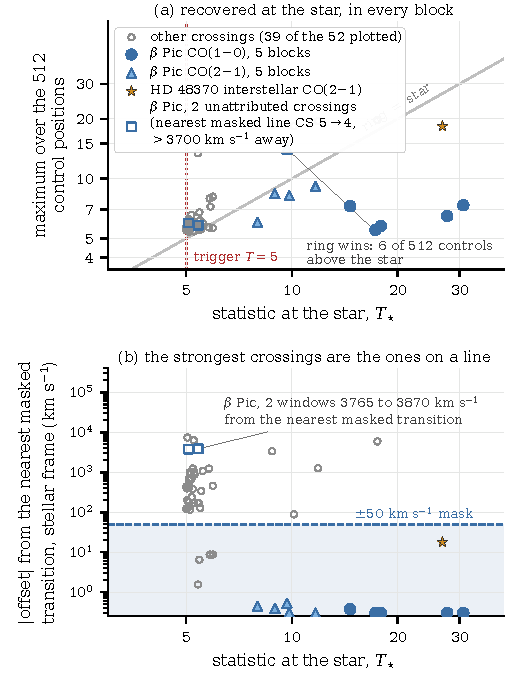
\includegraphics[width=\columnwidth]{figures/bpic_control.pdf}
%% ★★★ v4.26 (r25-captions): 16 PRINTED LINES -> R1 §7's limit of about six.
%% NINE macros had this caption as their only citation site.  Four --
%% \BpCtrlBlock, \BpCtrlBand, \BpCtrlRingMax, \BpCtrlStar -- went to
%% \S\ref{sec:bpicval}, into the sentence about the one block whose ring
%% beats the star, which described that block without naming it; the other
%% five -- \BpicPanelNDrawn, \BpicDvCoLo, \BpicPanelNCs, \BpicDvCsLo,
%% \BpicDvCsHi -- are the paragraph above, where this figure is introduced.
%% DELETED: the methanol offsets, which Appendix~\ref{app:linemask} states
%% in full and at greater length (\ZmOffLoMHz, \ZmOffHiMHz keep their sites
%% there), and "\NStageOneBpicEb{} of them with the star above every control"
%% which \S\ref{sec:bpicval} already carries.
\caption{The $\beta$~Pictoris positive control, in both directions
(\S\ref{sec:bpicval}). \emph{(a)}~The spatial screen: the stellar statistic
against the maximum over the window's \NCtrl{} control positions, filled for
the blocks recovering $\beta$~Pictoris CO. \emph{(b)}~Velocity offset from
the nearest masked transition \emph{in the star's own frame}, the adopted
$\pm\MaskHalfKms$\,km\,s$^{-1}$ half-width marked; grey, the
\BpicPanelNOther{} others, HD~48370 labelled.}
\label{fig:bpiccontrol}
\end{figure}
%
%% The line mask, reported in two layers: the frequency coincidence, which is
%% a velocity criterion and nothing else, and the one species we do not read
%% as emission, which is an argument and is set out as one.
%% Owner: r16-mask.  Carries \label{app:linemask} (cited by 04_method.tex and
%% app_C_spatialnorm.tex) and \label{tab:masklines}.
%%
%% ★ THIS APPENDIX IS THE PAPER'S ONLY DEFINITION OF THE ATTRIBUTION RULE.
%% It owns the species list, the half-width and the FRAME.  The rule is the
%% star's own rest frame; the local standard of rest is evaluated as a check
%% and changes no disposition (masklsr_v520.py, L10).  Sec. 5.3 states the
%% rule in one clause and Appendix D points here; nothing else in the paper
%% may name a frame of its own, or there are two rules again.
\section{The line mask}
\label{app:linemask}

A crossing that falls on a known molecular transition has an astrophysical
explanation to hand, and the mask exists to say which crossings those are. It
reports the frequency coincidence and the judgement about the coinciding
species separately, so the reproducible part can be recomputed and the
arguable part argued with.

\emph{The list, and when it was made.} The mask holds every transition of the
\FrNSpec{} species these spectral setups cover -- the three CO isotopologues,
HCN, HCO$^{+}$, CS, CN, SiO, H$_2$CO, [C\,\textsc{i}] and hydrogen
recombination -- that falls inside one of the \McNIsland{} searched frequency
intervals with an upper-state energy below \McEuMax\,K. That rule is the whole
of it, and it admits \FrNTrans{} transitions (Table~\ref{tab:masklines}).
No strength cut is applied across species: any threshold admitting HCN's
strong lines would discard the brightest lines in these fields. Within a
species the main hyperfine components are kept and the satellites
dropped. The list is a single Splatalogue query
\citep{Splatalogue2007} of CDMS and JPL \citep{Pickett1998,CDMS2005} made on
\MkListDate{}, and the query is dated and repeatable, so the mask itself can
be rebuilt.

\emph{The species are the ones the observers went to the telescope for, and
that is a limitation.} The spectral setups are tuned to them: \TnCenPct{} per
cent of the \NWinA{} Class~A windows are centred within
$\pm\MaskHalfKms$\,km\,s$^{-1}$ of a transition of the list and \TnWinPct{}
per cent contain one somewhere, while the same windows displaced bodily by
\TnShiftLoGHz{} to \TnShiftHiGHz\,GHz leave only
\TnCtrlCenLo--\TnCtrlCenHi{} per cent centred on one. The list is therefore
set by the science goals of the programmes that took
the data and not by anything in this search, and \emph{unattributed} means
unattributed against it. A wider list measures what that costs: every
transition below \XlEuMax\,K of all \XlNSpecies{} species with a published
interstellar or circumstellar detection, queried from CDMS and JPL
\citep{Pickett1998,CDMS2005} on \XlQueryDate, gives \XlNTrans{} transitions
inside the searched intervals, covering \XlBandPct{} per cent of the Class~A
union against \MkMaskAPct{} per cent for the list adopted here and
attributing every one of the \MkUnattr{} unattributed crossings together with
\XlShareWidePct{} per cent of the control positions' own exceedances, so it
empties the category for star and control alike. Narrowed to
$\pm\XlTightHalf$\,km\,s$^{-1}$, where it still covers only
\XlTightBandPct{} per cent of the band, it would attribute \XlTightNIn{} of
the \MkUnattr{} and the unattributed count remains what the control positions
predict (\XlTightObs{} against \XlTightExp{} expected); the nearest
transition of that wider list, with its quantum numbers, upper-state energy
and offset in both frames, is reported beside every unattributed crossing in
the accompanying data, so \emph{unattributed} can be read against it row by
row -- and at a density where \XlBandPct{} per cent of the band lies within
\MaskHalfKms\,km\,s$^{-1}$ of something, proximity is not an identification.

\emph{What an identification would look like, on the pair that comes closest
to one.} The \ZmNCross{} unattributed crossings of $\beta$~Pictoris lie
\ZmOffLoMHz{} and \ZmOffHiMHz\,MHz above components of the methanol
$5_K\to4_K$ ladder (\ZmCompLo{} and \ZmCompHi, $E_{\rm u}=\ZmEuLo$ and
\ZmEuHi\,K, at frequencies on which CDMS and JPL agree), \ZmDvLo{} and
\ZmDvHi\,km\,s$^{-1}$ in the star's frame: offsets agreeing with each other
to \ZmDvAgree\,km\,s$^{-1}$, which is the configuration a real line
identification produces and which arises by chance in \ZmChancePct{} per cent
of pairs drawn uniformly in the window they were found in. Four measurements
decide against it, all in the one window that holds both crossings and covers
the whole ladder in both blocks, \ZmBandLo--\ZmBandHi\,GHz in the stellar
frame. The brightest member of the complex, \ZmBright{} at
\ZmBrightMHz\,MHz, would reach $T_\star\ge\ZmPredAplus$ at any excitation
temperature and would therefore have been the window maximum, where the
maximum over the whole channel--drift grid is the crossing itself. The weaker
of the two claimed components cannot exceed \ZmRatioMax{} of the stronger at
any temperature and is observed at \ZmRatioObs{} of it. Both fitted drifts
are \ZmStepsLo{} and \ZmStepsHi{} steps of their own grid from the zero a
transition at rest requires, each track crossing \ZmSweepLo{} and
\ZmSweepHi{} channels inside its own block. And neither is present
\ZmGapH\,h later in the block covering the same frequency, where a persistent
line would be recovered at \ZmPersLo{} and \ZmPersHi$\sigma$ and the
statistic at that cell reaches only \ZmAnyLo{} and \ZmAnyHi{} over every
drift of the grid (\S\ref{sec:etacrv}). Where this system's own molecular gas
is seen, in \ZmCoNBlock{} blocks, it registers to \ZmCoReg\,km\,s$^{-1}$ of
rest.

\emph{Attribution is decided in the star's own rest frame, and the sign is
not the usual one.} A crossing's frequency is carried from the topocentric
value to the barycentre using its own block's pointing and mid-time, and then
to the stellar rest frame using the star's systemic velocity. That frame, and
no other, is where a coincidence is judged.
The barycentric term alone spans \FrBarySwing\,km\,s$^{-1}$ across the
survey, so a tolerance applied in the observed frame would spend most of its
budget on the Earth's motion. The \FrEpochNEpoch{} \FrEpochStar{} epochs show
the transform working in the only way that can be checked:
\FrEpochTopoKms\,km\,s$^{-1}$ apart as observed, they agree to
\FrEpochStelKms\,km\,s$^{-1}$ in the star's frame.
Throughout, $\Delta v_\star = c\,(\nu_\star-\nu_0)/\nu_0$, so a positive
offset means the crossing lies \emph{above} the transition
in frequency, the opposite sign to the velocity convention of a spectral line.

\emph{Every crossing is read in the local standard of rest as well, where
interstellar gas is at rest, and that second reading
establishes which coincidences are interstellar.} Of the \LsNLos{} stars carrying crossings, the composite
CO($1\to0$) survey of \citet{DameThaddeus2022}, which contains
\citet{Dame2001}, covers \LsNLosCov{} and holds emission toward \LsNLosDet{}
of them, between \LsCoVLo{} and \LsCoVHi\,km\,s$^{-1}$. Toward every other
star, including the \LsNLosOut{} outside the CfA footprint, the all-sky
Planck CO map \citep{PlanckCO2016} stays below
\LsPlanckMax\,K\,km\,s$^{-1}$. Toward
\LsCloudStars{} the CO spectrum is non-zero at the crossing's own LSR
velocity, within \LsCloudDvMax\,km\,s$^{-1}$ of its own peak and at
\LsCloudTMin\,K or brighter against a \LsCoRms\,K channel. So \LsNCloud{} of
the \MkNCoinc{} coincidences are interstellar gas and not circumstellar.
Two are worth naming. \BkAlmaName{} is a serendipitous field star toward the
Lupus clouds, at \BkAlmaDistPc\,pc with the clouds far behind it; its
CO($2\to1$) crossing lies \LsLupDv\,km\,s$^{-1}$ from a
\LsLupWco\,K\,km\,s$^{-1}$ cloud line at \LsLupVco\,km\,s$^{-1}$, so the
field is a molecular sightline and not a disc, and on such a sightline the
wider chemistry a molecular cloud carries is a real limitation: of the
species a Lupus line of sight would be expected to show, \XlLupNamedN{}
reaches one of its crossings within the mask's own half-width,
\XlLupNamedMol{} at \XlLupNamedDv\,km\,s$^{-1}$. HD~48370 is
the case where the two readings part: its coincidence lies
\LsHdDvStar\,km\,s$^{-1}$ from the star's own CO($2\to1$), while in the local
standard of rest it sits at \LsHdVfeat\,km\,s$^{-1}$, on a catalogued cloud
line peaking at \LsHdVco. The offset follows the interstellar gas and not the
star, so that window's extended emission is an interstellar cloud and not
a resolved disc.

\emph{A coincidence is an attribution, and for most of them it is not the
only evidence.} \LnAttrSupp{} of the \MkAttr{} attributions carry support
beyond the frequency match: catalogued carbon monoxide on the sightline here,
a second transition of the same species, or the crossing's own recurrence.
The other \LnAttrCoincWord, toward \LnCoincStars, rest on the coincidence
alone -- no catalogued gas on either sightline, no second transition and no
repeat epoch that recovers them -- so they are consistent with molecular
emission and are not identified as it. Table~\ref{tab:masklines} gives the
mask species by species; the hydrogen recombination lines among them carry
no tabulated upper-state energy, and are blank in that column.

\begin{table}
\centering
\footnotesize
%% ★ v4.26 (r25-captions): 4 printed lines -> the author's 3.  The hydrogen
%% recombination lines' missing $E_{\rm u}$ MOVED to the paragraph above: it
%% explains a blank cell, which is a fact about the catalogue and not a
%% definition of a column.
\caption{The line mask, by species: the number $N$ of transitions, the
frequency range they span inside the searched intervals and their
upper-state energies.}
\label{tab:masklines}
%% GENERATED by maskso_v414.py -- do not hand-edit.
\begin{tabular}{@{}lrr@{\,}c@{\,}rr@{}}
\hline
Species & $N$ & \multicolumn{3}{c}{$\nu_0$ (GHz)} & $E_{\rm u}$ (K) \\
\hline
H & 5 & 92.03 & -- & 231.90 & -- \\
H$_2$CO & 13 & 101.33 & -- & 491.97 & 10--106 \\
C$^{18}$O & 3 & 109.78 & -- & 329.33 & 5--32 \\
CN & 50 & 113.12 & -- & 680.30 & 5--114 \\
CO & 3 & 115.27 & -- & 345.80 & 6--33 \\
CS & 3 & 195.95 & -- & 342.88 & 24--66 \\
SiO & 2 & 217.10 & -- & 347.33 & 31--75 \\
$^{13}$CO & 8 & 220.40 & -- & 330.59 & 16--32 \\
HCN & 7 & 354.50 & -- & 354.51 & 43--43 \\
HCO$^{+}$ & 1 & 356.73 & -- & 356.73 & 43 \\
{[C\,\textsc{i}]} & 1 & 492.16 & -- & 492.16 & 24 \\
\hline
\end{tabular}%

\end{table}

\emph{The coincidences, and the one species the mask leaves out.} Of the
\NCross{} crossings, \MkNCoinc{} fall within $\pm\MaskHalfKms$\,km\,s$^{-1}$
of a transition of the list in their own star's frame. The list holds no
species whose coincidences are reported and not acted on, so those are also
the \MkAttr{} attributions and the two counts are one count. Sulphur monoxide is a catalogued species of these spectral
setups and is deliberately not in the list: no debris disc has a reported SO
detection, where the second-generation gas is CO, C and O, so masking its
\SoNTrans{} transitions would have declared no constraint over bandwidth this
survey does constrain. That leaves \SoNCrossWord{} crossings within the same
half-width of one of them -- \SoStars, at \SoDvList\,km\,s$^{-1}$ from
transitions of upper-state energy \SoEuLo--\SoEuHi\,K -- and all
\SoNCrossWord{} are therefore searched, tested and reported as unattributed,
with the offset printed beside each in the ledger. \SoNBelowScreen{} of them
are below the rank screen as well.

Interstellar sulphur monoxide is another matter, and it is a measurement
rather than a preference. It is a common molecular-cloud species, \LsNCloud{}
of the \MkNCoinc{} coincidences here are interstellar rather than
circumstellar, and a crossing on such a sightline could be interstellar SO
rather than noise. Interstellar gas is at rest in the local standard of rest,
where the three offsets are \SoDvLsrList\,km\,s$^{-1}$, so for one of them
the coincidence does not survive the change of frame at all. \SoNUncovered{}
of the three lie outside the footprint of the composite CO($1\to0$) survey and
their sightlines carry at most \SoPlanckMax\,K\,km\,s$^{-1}$ of integrated
CO against the \SoPlanckCeil\,K\,km\,s$^{-1}$ a detection needs. The third,
\SoCloudStar, is a molecular sightline -- the survey detects
\SoCloudTpeak\,K at \SoCloudVpeak\,km\,s$^{-1}$,
\SoCloudW\,K\,km\,s$^{-1}$ integrated, at $l=\SoCloudGlon^{\circ}$,
$b=\SoCloudGlat^{\circ}$ -- but its crossing sits at
\SoCloudVfeat\,km\,s$^{-1}$, \SoCloudDv\,km\,s$^{-1}$ from that emission,
where this survey's own cloud test allows \LsCloudDvMax\,km\,s$^{-1}$. Each
of the three windows also covers CO($3\to2$), and in each the maximum over the
whole channel--drift grid is the crossing itself, so no CO($3\to2$) feature
above the trigger accompanies any of them -- and carbon monoxide, not sulphur
monoxide, is what a cloud shows first. The reserved hold-out is treated
identically, leaving \HoNAttr{} attributed and \HoNUnattr{} unattributed
there (\S\ref{sec:holdoutsearch}).

\emph{The half-width, and what it costs.} A one-channel test is too tight for
circumstellar gas, whose emission is shifted by many channels: the width
follows from Keplerian motion where these molecules survive,
$\lesssim$13\,km\,s$^{-1}$ beyond 10\,au, and is
$\pm\MaskHalfKms$\,km\,s$^{-1}$. At that width the mask removes
\MkMaskAGHz\,GHz of the \CvUnionA\,GHz Class~A union, \MkMaskAPct{} per cent
of it, and \FrMaskLostGHz\,GHz of \FrMaskUnionGHz\,GHz over both classes
together, \FrMaskPct{} per cent, so the cost falls on the primary
experiment, because its windows are the line-tuned ones.
Attributing on either frame instead would mask the union of two tubes
separated by the star's LSR velocity, \LsMaskTwoGHz\,GHz or
\LsMaskTwoPct{} per cent of the Class~A union -- \LsMaskAddPct{} per cent
more bandwidth for no further attribution, which is the measurement behind
deciding in one frame. Between $\pm\FrLadderLo$ and
$\pm\FrLadderHi$\,km\,s$^{-1}$ the mask attributes \FrAttrWTwenty{} to
\FrAttrWHundred{} of the crossings, and the \FrNRankPass{} that outrank
every control position of their own windows are the same two at every
width.

\emph{The labelled crossings are tested for recurrence too.} \MkAttrTested{}
of the \MkAttr{} attributed crossings have a later block covering the
predicted cell, and the \MkAttrRecur{} that are present again, toward
\MkAttrRecurStars, are the positive control of that stage; \MkAttrUntest{}
have no covering block at all (\MkAttrUntestNames). For the \MkAttrExcl{}
not recovered a repeat window's own largest statistic bounds the predicted
cell from above and the ledger prints the row as a bound, at
$T_{\rm rep}<\RqHrTRep$ and $T_{\rm rep}<\RqAjTRep$ against the
$T_{\rm pers}=\RqHrTPers$ and $T_{\rm pers}=\RqAjTPers$ real carbon
monoxide at the discovery flux density would have given. One of those two
attributions rests on a velocity rather than on the recurrence test, the
sightline carrying catalogued interstellar emission
\LsLupDv\,km\,s$^{-1}$ from the crossing's own LSR velocity, and its repeat
blocks show where that gas lies rather than whether it can be recovered:
in every one of them between
\RqAjNgeLo{} and \RqAjNgeHi{} of the \NCtrl{} control positions stand above
the star, so the gas is bright and it is not at the star.
%
%% APPENDIX D -- the false-alarm expectation, the control ensemble, and the
%% execution-block quality criterion.  Owner: r14-chance.  Carries
%% \label{app:falsealarm} (04_method.tex, 08_backmatter.tex) and
%% \label{sec:blockquality} (04_method.tex).
\section{The false-alarm expectation and the control ensemble}
\label{app:falsealarm}

This appendix gives the chance expectation for the unattributed crossings,
what it is conditioned on, and what the control ensemble calibrating it can
support.

\subsection{Conditions on the expectation}

\emph{One attribution set serves both sides of the comparison}, the set of
\S\ref{sec:technosearch}: the mask of Appendix~\ref{app:linemask} within
$\pm\MaskHalfKms$\,km\,s$^{-1}$ in the star's own rest frame, which holds no
sulphur monoxide. So the \SoNCrossWord{} crossings that fall on SO transitions
are unattributed crossings, and a control maximum on one of those transitions
is an unattributed exceedance: the same list on both sides, as it always was. A systemic velocity is measured for the stars of
\CeNVsys{} of the census windows and the others are taken at rest, which moves
the masked share by \CeVsysSensPct{} points.

The expectation is built from the control positions, the only empirical null
the data provide, and each Class~A window contributes two quantities
measured on itself. The fraction of its own \NCtrl{} control positions that
reaches the trigger is the probability that a position in that field does so
-- no cell count enters it and no form is assumed for the tail -- and
summed over the windows \CeExpTrig{} are expected to trigger by chance. How
many of those would be attributed is measured on the channels the control
maxima land on, which the retained spectra record: \CeNExcAttr{} of
\CeNExc{} exceedances fall inside the mask -- carried to the same star's rest
frame, through the same two steps and against the same transition list as a
cell at the stellar position -- and the attribution therefore
takes \CeMaskPct{} per cent of the expectation, where a maximum free to
land anywhere on its own grid would take \CeUnifPct{} per cent: the
\CeNFullMask{} narrow line-tuned windows lie wholly inside the mask and
their fields, which hold real emission, are where a control position most
often triggers, so a uniform landing would under-attribute them and leave
the unattributed expectation too high. The atmospheric screen of
Appendix~\ref{app:rfi} is then applied to these same positions, on the same
radius and in the same topocentric frame as to the crossings, and takes
\CeTlCtrlCut{} of the \CeTlCtrlSurv{} exceedances the mask leaves, a further
\CeTlPct{} per cent. That leaves \CeExp{} expected unattributed Class~A
crossings against \CeObs{} observed.

Both sides run over the \CeNWin{} Class~A windows of the primary census, so
the expectation is a sum over rows and nothing is carried at an assumed rate.
They are also read over the same field, and which field that is matters.
The $\sigma$ of Equation~\ref{eq:tstar} is the median absolute deviation over
the control positions, so $T_\star$ is a property of the annulus as much as of
the cell: one product supplies both sides here, the statistic read over the
whole primary beam with each block on its own antenna geometry, for the
expectation and for the crossing count alike. A field narrower than the
primary beam drops the integrations whose pointing falls outside it, and with
them on-source time and real signal, so a statistic read over part of a beam
is not the quantity \S\ref{sec:statistic} defines. The choice is not
immaterial and is reported rather than assumed small: read over such a field
on both sides, the same comparison gives \FrNarrowObs{} crossings against
\FrNarrowExp{} expected at $P=\FrNarrowProb$, where the whole beam gives
\CeObs{} against \CeExp{} at $P=\CeProbNull$; the bound below becomes
\FrNarrowAddLim{} further crossings against \CeAddLim{} on the same
resampling. The same comparison holds system by system, each system's
expectation formed from its own control positions: \MtNSysLowP{} of the
\MtNSysChance{} systems fall below one chance in twenty, against
\MtNSysLowPExp{} expected, and no system departs from its own controls by
more than chance allows.
A further \CeNWinTail{} searched Class~A windows lie outside the comparison
because the deposit does not tabulate them -- \VnTailNWinA{} in the
archival-tail blocks of \S\ref{sec:sample} and \VnCompNWinA{} toward a
companion resolved after the census closed -- together with the
\CeNTailCrossWord{} unattributed crossings toward \CeTailStar{} they hold,
which are reported beside it and enter neither side. No window holds more than one primary crossing, so
both sides count windows; the weaker cells behind those maxima are counted at
their own grain in \S\ref{sec:technosearch}.

The one assumption the searched data cannot test is that a star behaves like
a control position in its own field, and two samples measure it. In the census
the star carries \CeNear{} times as many above-threshold cells as a control
position of the same field, measured in the band immediately below the
trigger, $\CeNearBandLo\le T<\CeNearBandHi$, on \CeNearNStar{} stellar cells
over the \CeNearNWin{} windows that retain a control vector, with
\CeNearIntLo--\CeNearIntHi{} allowed at \CeCovPct{} per cent when the
execution blocks are resampled. The band ends at the trigger because the
ratio is not flat in level: read half-level by half-level it rises from
\CeNearRiseLo{} to \CeNearRiseHi, so a band further below the trigger would
not measure it where the comparison uses it. No cell under test enters it, a
band count being the difference of two cumulative counts, so an
above-threshold cell belonging to a crossing is counted in both terms and
cancels; at the trigger itself the ratio is \CeTrAt, but there it is formed
from the \CeStepNX{} cells that are the crossings under test. No step is
applied to the sum above: the expectation adopted is the control positions'
own, the smaller of the two and the more demanding of the count under test.
Carried in as a sensitivity test it raises the expectation to \CeExpNear{}
and the probability to \CeProbNear{} and lowers the bound to \CeAddLimNear,
the control positions' own rate being the one adopted.
What the comparison requires of that ratio is a statement in
the other direction: the \CeObs{} observed would stand above chance at the
\CeAlphaPct{} per cent level only if stars reached the trigger at \CeRCrit{}
times the rate of a control position or less, a deficit at the star of
\CeRCritPct{} per cent, and every ratio measured here is an excess instead.
The reserved blocks measure
the same quantity on blocks the search did not reach: their stars reach the
trigger in \StHoObs{} of \StHoNFine{} fine-channel windows where the control
positions of those same windows predict \StHoExpFine, a ratio of
\StHoRatio, and in the \StHoNCoarse{} coarse-channel reserved windows no
star reaches it against \StHoExpCoarse{} predicted. Every one of those
events lies in a reserved block that shares an observing session with a
searched one, and the \HsIndBlocks{} reserved blocks that share none hold
\HsIndObsWord{} trigger \HsIndObsNoun{} between them, so they neither
confirm the step nor contradict it (Appendix~\ref{sec:heldout}).

A count is compared with the distribution of counts chance delivers, and
not with a range on its own mean. A rate is drawn from \CeNBoot{} resamplings
-- each window's rate redrawn from its own \NCtrl{} probes, the attributed
share from its own \CeNExc{} exceedances, and the execution blocks resampled
because windows share them and are not independent trials -- and the count
scatters about that rate. A count of \CeObs{} or more then arises with
probability \CeProbNull{} at the control positions alone, and that is the
comparison adopted here; as a sensitivity test, applying the step gives
\CeProbStep. The same distribution bounds what the comparison could have
missed: added to each resampled control-position rate, \CeAddLim{} further
crossings still leave a count as low as \CeObs{} credible at \CeProbAtLim,
and one more does not, at \CeProbAboveLim{} against the \CeAlphaPct{} per
cent level. So \CeAddLim{} is the largest added population this comparison
could not have rejected, the uncertainty in \CeExp{} carried inside it by the
same resampling, and it is the compatibility statement of
\S\ref{sec:trigunif}: it counts crossings and not transmitters. Read at the grain of
the individual cell rather than the window, the same accounting gives
\CkExp{} expected against \CkNObs{} found, with \CkLo--\CkHi{} covering
\CeCovPct{} per cent of the same resampling.

\subsection{Execution-block quality}
\label{sec:blockquality}

The comparison with the control positions assumes each block's ensemble
behaves like noise, and one block makes that false: every one of its \NCtrl{}
probes exceeds the trigger, the smallest at \BqFailCtrlMin. A criterion for
the condition is therefore applied to every block and not to the one that
prompted it.

\emph{Two criteria are built from that statistic and they are not the same
test.} The statistic is the median of a window's own \NCtrl-position control
ensemble, which separates a field with a source in it from a field that is no
null at all. A \emph{window} is flagged when that median exceeds \BqFactor{}
the survey median of the same quantity, \DqThresh{} against \DqSurvMed; the
flag is a property of the window and cuts across attribution by design,
firing on \DqNWin{} of the \NWindows{} windows in \BkFlagNBlock{} blocks
toward \DqNStar{} stars (\DqStars), every one of which carries a crossing.
A \emph{block} is judged on the same median divided by the median over the
windows of its own class, since a maximum over a larger channel$\times$drift
grid sits higher; it fails where the median of that ratio over its windows
exceeds \BqFactor{} the scale of its class. The factor is the same in both.

\emph{Neither criterion was fixed in advance.} The condition was noticed
in one block and the criterion written afterwards, so it is post hoc, and
what makes it trustworthy is how little the position of the line matters. The
failing block sits at \BqFailQ{} and the next most extreme at \BqNextQ, a
factor \QsRatio{} apart; over \QsNStep{} thresholds spanning that interval
the same single block is selected every time, in number and in identity, so
the line may be drawn anywhere from \QsMarginLo{} to \QsMarginHi{} times
where it is. Outside that interval the answer does change, which is how one
can tell the rule discriminates: at \BqNextQ{} it selects \QsNAtNext{}
blocks, and at the median block, \QsQMed, \QsNAtMed{} of the
\BqNBlocks. Nor does the class treatment decide it: the same block is
selected with each class normalised on its own windows and with the survey
taken as one, and no block in the census is failed on one class
and passed on the other. The median block of the primary census sits at
\BqQMed, nothing else is close to the \BqNFail{} the criterion fails, and the
unscaled form of the rule fails the same \BqRawNFail{} block. Its
\BqFailNWin{} windows are all coarse-channel and
hold the survey's entire Class~B crossing population, so it carries
\EvNCrossFlag{} of the \EvNCrossRaw{} threshold crossings. \EvNRankFlag{}
of those outrank all \NCtrl{} control positions of their own window, and
no Class~A statistic here has ever contained it. Those \EvNCrossFlag{} appear
in the crossing ledger with their block named and enter no count
elsewhere.

\subsection{The control ensemble's resolution}

Over the \VerNTested{} census windows that retain a control vector the
stellar ranks are consistent with the one half exchangeability implies --
median \BkRankBalSurv{} with each star carrying equal weight,
\BkRankBalSurvLo{} to \BkRankBalSurvHi{} at \CeCovPct{} per cent -- which is
a weak statement and not a strong one, since a shift smaller than about
\VerKsPowerAca{} could not have been seen in a sample of this size, and the
reserved blocks agree once each star carries equal weight, \BkRankBalHo{}
(\BkRankBalHoLo--\BkRankBalHoHi). \emph{The rank is not a significance test,
and the reason is structural.}
Ranking the star against \NCtrl{} control positions of the same field
decides which windows deserve examination, but $1/(\NCtrl+1)=\RankFloorVal$
is the \emph{resolution} of the ensemble -- the smallest rank it can
express -- and not the probability that noise produced the window. A survey
of \NWindows{} windows would need a rank \BonfRankRatio{} times finer, and
correlation makes it coarser still: controls inside the synthesised beam are
not independent, so an annulus resolves no better than
\RankEffLo--\RankEffHi{} however many probes are drawn into it, with the
primary beam bounding how many a single pointing contains. That floor is the
design's central limitation: no single window here can be significant on the
rank alone, which is why confirmation requires independent recurrence.

\subsection{The trials budget}

The searched cells counted in \S\ref{sec:summary} are not independent
trials: channel smoothing and a drift grid stepped twice per channel
correlate neighbouring ones, which alone would leave \StGridFrac{} of them
independent, while fitting each window's effective count against its own
control ensemble returns \StNindFrac{} and those ensembles' maxima sit at
\CtrlMaxRatioMed{} of the prediction for the maximum of the full searched
count treated as independent and Gaussian. Nothing
turns on which is right, because the expectation above is summed from measured
rates and not from a cell count: by the cell-count route the number reaching
the trigger is \StExpModel{} against \CeExpTrig, \StModelAgreePct{} per
cent away. The on-star crossings do exceed a Gaussian tail over every
searched cell, which predicts \CellExpect{} stellar exceedances against the
\NCross{} found -- but \MkAttr{} are attributed by the set above,
\EvNCrossFlag{} come from the block of \S\ref{sec:blockquality},
\CeNTailCross{} fall outside the census windows and \CeTlObsCut{} is
atmospheric, which leaves \CeObs{}
against the \CeExpSurv{} the same control positions predict over both classes
together -- the \CeExp{} of the fine class and the \CeExpCoarseAdd{} the clean
coarse windows add to the expectation while holding \CeObsCoarseWord{} crossing
of their own, which is what keeps the comparison symmetric --
so no excess survives the attribution. The remainder is bounded and
the bounds are null: the measured stellar ranks agree at $\pv{\StarPseudoP}$
with the \NPseudo{} ranks each control takes against the other probes of its
own window, radial suppression is below \RingRhoBoundPct{} per cent in the
mean, and scrambling a window so nothing coherent survives along a drift
track carries \LNNWindows{} past the rank floor and changes no disposition.

%% The chance expectation here is summed from the measured control exceedance
%% rates and each window's own masked grid share (chance_v414.py, round 310),
%% so no cell count and no Gaussian tail enters it and nothing in it is
%% conditioned on the crossings; the cell-count route is a cross-check only,
%% and the rank-conditioned expectation (\ClustStageMean against
%% \ClustStageNObs) is a pipeline diagnostic that must not be reachable as
%% "the" expectation.  tab:ctrlsep, tab:excess, tab:arraysplit and
%% fig:ctrldiag are generated and nothing cites them; r15-deposit, 2026-10-08:
%% they used to be described as "in the data release", and there is no data
%% release, so they are simply unpublished diagnostics.
\subsection{The registration of the predicted cell}
\label{sec:regbudget}

The recurrence test of \S\ref{sec:etacrv} reads one channel at one drift
rate, so what it can conclude depends on how well that cell is registered
between two epochs. Every term of the budget is a frequency the reading
knows to a fraction of a channel: half a channel for the predicted cell,
half for the discovery channel it is referred to, \RgDriftWithinChMed{}
for the drift, \RgVsysChMax{} for the systemic velocity, which is removed at
one epoch and re-applied at the other, and \RgBaryChMax{} for the ephemeris,
a total of \RgBudgetChMed{} of a channel in every window and
\RgBudgetKmsMed\,km\,s$^{-1}$ in the median one. The frame correction is the
one term that is large in channels rather than small: it moves the predicted
cell by up to \ZtFrameChanMax{} channels, and by $\VnEcrDchan$ for
$\eta$~Crv. No reading at all is quoted for \RcUntStar{} \texttt{\RcUntEb},
whose frequency \RcUntNRep{} blocks cover but whose own window retains no
spectrum, so there is no discovery amplitude to transport to them. That is a
budget and not a
measurement, and the measurement is larger where the channels are narrow: the
stellar-frame centroid of a real recurring line sits a median
\RgCenMedKms\,km\,s$^{-1}$ from the predicted cell and \RgCenMaxKms{} at
worst, measured over \RgCenNBlock{} block readings of the line-attributed
recoveries. Each exclusion was therefore re-read over every cell within
\RgTolKms\,km\,s$^{-1}$ of the predicted one -- \RgNTrialMax{} cells at most
-- and formed from the worst of them, with the threshold raised to
\RgThrMax{} so that the wider reading keeps the single cell's own false-alarm
probability; it costs depth, the amplitude ruled out falling from a median
\RcFracMed{} to \RgFracMed{} of the discovery amplitude, and \RgNVac{} of the
\RcNExcl{} then rule out nothing, both of them already among the
\HjNPowerLo{} crossings \S\ref{sec:etacrv} reports as untested and not
excluded. Reading the same cell at every trial of the window's own drift grid
instead, which bounds an error in the carried drift whatever its size, leaves
the largest value anywhere \RcTMax{} over all \RcNRepeatMeas{} readings. The
reading has also to be pinned somewhere along the track, because a drifting
carrier occupies tens of channels and not one: each observation is de-drifted
from its own first integration, and pinning the cell anywhere across the span
the discovery track covers moves it by at most \AnSpanMaxKms\,km\,s$^{-1}$,
where the nearest above-trigger cell in any covering window lies
\AnNearKms\,km\,s$^{-1}$ away and the strongest reading over every anchor is
\AnTBest{} combined and \AnTSingle{} in a single block. So no disposition
rests on the carried drift, on the anchor or on the width of the cell.
Combining every covering block is what buys the depth that is quoted: the
nearest block alone rules out a median \TjFracNearMed{} of the discovery
amplitude, and \TjNNearWeak{} of the \RcNExcl{} rule out nothing on it. One
window is delivered twice by the archive, once with the control annulus on
that compact-array block's own antenna geometry and once on a nominal 12\,m
beam: the reading on the block's own geometry is the one published,
\LrSuppPub, where the 12\,m annulus gives \LrSuppOwn{} for the same cell,
\LrSuppPct{} per cent apart, \NbProvRmsPct{} per cent of that in the window
noise and the rest in the recovered amplitude. Part
of the power the single cell loses is the threshold and not the archive: a
statistic of five was set for a window of $10^{\TuCellsDecLo}$ to
$10^{\TuCellsDecHi}$ cells, and at
one predicted cell it is a far stricter demand, a false-alarm probability of
$\ZtOneCellP\times10^{\ZtOneCellExp}$ evaluated at the scatter measured in
\S\ref{sec:nullscatter}; holding the chance of a single false confirmation
across all \RcNRepeatMeas{} readings at \ZtFwPct{} per cent instead puts the
bar at \ZtTrialThr, and nothing would have been confirmed there either, the
largest single-block reading at the carried drift being \RcTMatched. A
carrier that keeps drifting across the gap is a different model and the
numbers belong to it: at the rates fitted here such a carrier is a median
\RgWalkChMed{} channels from the predicted cell by the nearest covering
block, and $\RgWalkChMax\times10^{\RgWalkChMaxExp}$ at \RgWalkStar.

\subsection{From the widened window's exceedances to the pairs}
\label{sec:pairacct}

Two counts of \S\ref{sec:etacrv} are counts of different objects, and
Table~\ref{tab:pairacct} takes one to the other. The \WdNExc{} above-trigger
readings are window readings, one for each pairing of an unattributed
crossing with a window that covers its frequency in another block, so a pair
whose two members are both unattributed crossings is read twice:
\PaNPairTwice{} of the readings are such a second reading, representing
\PaNPairRead{} distinct pairs, of which \PaNPairBeyond{} lie outside the
interval the pair test admits -- the median covering window's half-width --
and \PaNPairInside{} remain, which is the set Table~\ref{tab:pairs} is formed
over. The observatory's own line-of-sight acceleration is removed from both
fitted drifts before they are compared, at most \TjFrameMaxHzS\,Hz\,s$^{-1}$
here. Of the \TjNPower{} pairs whose rates the grid resolves, every one fails
a drift changing at a constant rate, by \TjSigMin{} standard deviations in
the mildest case; the offset
$\frac{1}{2}(\dot\nu_1+\dot\nu_2)\Delta t$ such a
trajectory predicts has no freedom left once both rates and the interval are
fixed, and the pair the searched grid itself separates is \EcGridStar's,
whose two crossings lie \EcGridDvKms\,km\,s$^{-1}$ apart in blocks
\EcGridDtH\,hours apart, a single carrier having had to drift at
\EcGridFactor{} times the grid's ceiling between them. Nothing measured here
bounds the curvature in between: the ceiling bounds the line-of-sight
component of a carrier's acceleration and not how fast that component can
turn over, an orbit directed across the plane of the sky sweeping it
\EcRateSupFac{} times faster than the circular orbit at the ceiling, while
the velocity excursion \emph{is} bounded, to within \EcVsupFac{} times the
circular amplitude over every eccentricity and orientation, which is why the
widened window of \S\ref{sec:etacrv} can be set against that excursion and a
reversal time cannot. The control row is a line
that does not drift: the \TjCtlLine{} line of \TjCtlStar{} is recovered at
one stellar-frame frequency \TjCtlDtD{} days apart and \TjCtlNSig{} standard
deviations from the prediction, its fitted drifts \TjCtlDriftStep{} of one
\TjCtlStepHzS\,Hz\,s$^{-1}$ grid step from zero and the predicted offset
below the comparison's own resolution over the same interval, so the
comparison resolves a mean drift to \TjCtlDriftResHzS\,Hz\,s$^{-1}$ and no
finer at any baseline. For the \TjNOpen{} pairs it cannot separate --
\TjNPowerOpen{} of them resolved and failed by the constant-acceleration
comparison -- nothing measurable tells one carrier from two.

$\beta$~Pictoris is the closest case, and it is the one the comparison
cannot dismiss. Its two crossings sit at \TjBpNuLo{}
and \TjBpNuHi\,GHz, \TjBpDvKms\,km\,s$^{-1}$ apart in the star's frame, in
blocks \TjBpDtH\,hours apart -- both inside the methanol $5_K\to4_K$ ladder,
which Appendix~\ref{app:linemask} excludes as their source -- with both
fitted drifts negative
($\TjBpDriftLo$ and $\TjBpDriftHi$\,Hz\,s$^{-1}$), so a single carrier would
have had to rise in frequency between the epochs and under constant
acceleration misses by \TjBpNSig{} standard deviations -- but the mean
acceleration it needs, \TjBpAccelReq\,m\,s$^{-2}$, is inside the
\WdAGrid\,m\,s$^{-2}$ ceiling. The pair fixes three numbers, the
acceleration at each epoch and the frequency offset between them, and a
circular orbit about a star of \EcMassBp\,M$_\odot$ \citep{Crifo1997} has
three free parameters: one orbit reproduces all three at once, at
\ObDayBp\,d in period, \ObIncBp$^\circ$ in inclination and \ObAuBp\,au in
radius, eccentric orbits fit up to $e$ of about \ObEccMaxBp{} before the
periastron acceleration leaves the ceiling, and the pair is therefore not
separable.

\begin{table}
%% ★ v4.26 (r25-captions): 5 printed lines -> the author's 3.  Naming
%% Table~\ref{tab:pairs} as what the readings are taken TO says in one clause
%% what two said: "the pairs the trajectory test is asked of" and "the counts
%% in the lower block are those of Table~\ref{tab:pairs}" are the same pairs.
\caption{The \WdNExc{} above-trigger readings of the widened recurrence
window, taken to the pairs of Table~\ref{tab:pairs}; each block of rows is
the one above with one effect removed.}
\label{tab:pairacct}
\footnotesize
%% GENERATED by pairacct_r23.py -- do not hand-edit.
\begin{tabular}{@{}p{0.76\columnwidth}r@{}}
\hline
Covering windows read, over the \PaNCovWinCross{} unattributed crossings a later block covers & \WdNCov \\
\ldots{} holding a statistic above the trigger, in \PaNRepWin{} windows of \PaNRepBlock{} blocks & \WdNExc \\
\hline
Distinct crossing pairs those readings represent & \PaNPairRead \\
\ldots{} readings that are the second reading of such a pair & \PaNPairTwice \\
Pairs separated by more than $\pm\WdHalfKms$\,km\,s$^{-1}$ in the star's frame, to \PaDvBeyondMax\,km\,s$^{-1}$ & \PaNPairBeyond \\
Pairs inside that interval & \PaNPairInside \\
\hline
Pairs with at least one unattributed member & \TjNCandPair \\
\ldots{} with a fitted drift and a block epoch for both members & \TjNPair \\
\hline
\ldots{} separated by the bounded-trajectory criterion & \TjNExcl \\
\ldots{} open & \TjNOpen \\
\hline
\end{tabular}

\end{table}

%% ★★ v4.23: THIS SUBSECTION AND ITS TABLE SIT AT THE END OF THE
%% APPENDIX FOR A REASON THAT IS NOT STYLE.  Placed next to the
%% registration budget, where it belongs by subject, its float took
%% the number Table~D1 and pushed the crossing ledger's sample to D2
%% and the recurrence positive controls to D3 -- and the positive
%% controls are the table Referee 2's first point is about, which he
%% and the response letter both call Table~D2.  Renumbering the
%% table a referee is reading about is a cost with no benefit, so the
%% new float goes last and takes the new number.  \S\ref{sec:edge}
%% is cited from \S4 and \S5.6 and the pointer is unaffected.
\subsection{The drift grid's edges}
\label{sec:edge}

The drift trials of a window run from $-\dot\nu_{\max}$ in equal steps of
half a native channel across the retained track, and the last trial is the
first at or beyond $+\dot\nu_{\max}$, so the interval searched is asymmetric
by up to one step and the ceilings themselves, computed window by window from
Equation~\ref{eq:accel}, reproduce it to $\DriftRelDev$ over all
\DriftRelNWin{} Class~A windows. Each window's grid is recovered from two
quantities that enter no common calculation -- the trial count recorded for
it and the channel width and retained span its own crossing record carries --
and the two agree on \EgNGrid{} of the \EgNDrift{} crossings that carry a
fitted drift, on every one of which the fitted rate is a trial of that grid
exactly; \EgNEdge{} lie on an outermost trial (Table~\ref{tab:edge}), toward
\EgEdgeStars, and are reported as lower bounds, while the remaining
\EgNNoGrid{} are in archival-tail windows for which no grid is recorded
anywhere.

\begin{table}
%% ★ v4.26 (r25-captions): 6 printed lines -> the author's 3.  DELETED after
%% checking: "a maximum at the boundary of the interval searched is a lower
%% bound" is \S\ref{sec:etacrv}'s own definition of \emph{edge-limited}, and
%% "Table~\ref{tab:pairs} gives them in the star's frame" is now a clause of
%% that same paragraph, which is where a reader meets both tables.
\caption{The crossings whose fitted drift lies on an outermost trial of
their window's own grid, with that grid. Rates are in the observatory
frame.}
\label{tab:edge}
\footnotesize
%% GENERATED by edge_v423.py -- do not hand-edit.
\begin{tabular}{@{}llr@{~}r@{~}c@{~}r@{~}l@{}}
\hline
Star & block & $\nu$ & $\dot\nu_{\rm obs}$ & trial & \multicolumn{2}{c}{$|a_{\rm los}|$} \\
 & & (GHz) & (Hz\,s$^{-1}$) & & \multicolumn{2}{c}{(m\,s$^{-2}$)} \\
\hline
BD+05~1668 & \texttt{X28a8} & 242.195 & $+3452$ & 2/2 & $\ge$ & 4.27 \\
HD~14055 & \texttt{X29ae} & 331.156 & $-3976$ & 0/135 & $\ge$ & 3.60 \\
HD~14055 & \texttt{X2c3bb} & 345.526 & $+4184$ & 141/141 & $\ge$ & 3.63 \\
HD~161868 & \texttt{X10ca8} & 345.634 & $+4195$ & 127/127 & $\ge$ & 3.64 \\
TRAPPIST$-$1 & \texttt{X259b} & 346.245 & $-4623$ & 0/137 & $\ge$ & 4.00 \\
\hline
\end{tabular}

\end{table}
%
%% APPENDIX E -- radio-frequency interference screening.
%% Owner: appendix-triage.  Carries \label{app:rfi}.
\section{Radio-frequency interference screening}
\label{app:rfi}

Interference is the first alternative explanation for an unattributed
crossing, so the screening this survey has and the coverage it lacks are both
set out here. Millimetre interferometry is an unusually poor
environment for terrestrial interference, though not an empty one: ITU Radio
Regulations Article~5 \citep{ITU2024} carries active allocations throughout
90--275\,GHz, and WRC-19 identified parts of 275--450\,GHz for land-mobile and
fixed use. The specific hazard is the \RadarLo--\RadarHi\,GHz Earth
exploration-satellite allocation used by spaceborne cloud radar
\citep{CloudSat2002,EarthCARE2023}, a documented contaminant of ALMA Band~3
\citep{ALMAMemo504}: of the \RadarNTot{} census windows \RadarNWin{} overlaps
it, carrying \RadarNCross{} threshold crossings and \RadarNStage{}
rank-passing events, so no result here rests on it. Two things favour this
band: terrestrial transmitters are sparse compared with centimetre
wavelengths, and an interferometer is not a total-power detector, so a signal
not in the far field at the phase centre acquires a rapidly varying
geometric phase across the array and is suppressed in the correlation rather
than imaged.

\emph{The coverage of the screening is uneven.} The five tests of
Table~\ref{tab:rfitests} are computed for every searched window of the
census, as is the \NCtrl-position rank screen; recurrence
reaches only the crossings with a covering repeat block, and the visibility
fit is a consistency check rather than a filter. The correlator flagging is
the observatory's own, replayed from each block's delivered calibration
script, and was not retained window by window: \emph{no per-channel
interference flag of our own exists, and none can be recovered.} The
populations of the five tests in Table~\ref{tab:rfitests} differ from one
another for that reason: each test needs a different quantity to have been
recorded.

\begin{table}
\centering
\footnotesize
%% ★ v4.26 (r25-captions): 4 printed lines -> the author's 3.  The reason the
%% five populations differ MOVED to the paragraph above, where the record
%% that is or is not retained is the subject.
\caption{The five interference tests, each of which could have failed. $p$ is
against the same peaks redrawn on their own channel grids.}
\label{tab:rfitests}
\begin{tabular}{@{}p{0.20\columnwidth}p{0.22\columnwidth}p{0.33\columnwidth}r@{}}
\hline
Test & Population & Result & $p$ \\
\hline
Clustering in sky frequency &
\AppMNCrossF{} crossings with a measured peak &
\AppMTubeObs{} within $\pm\DispoHalfKms$\,km\,s$^{-1}$ of a searched
transition against \AppMTubeNull{} expected: they cluster on the survey's own
lines &
\AppMTubeP \\
Crowding on one another &
\QcNQP{} unattributed, quality-passing &
no crowding at any of six separations from \QcTolLo{} to \QcTolHi\,MHz, where
the \QcNAttr{} attributed crossings crowd at every one &
$\geq\QcPQPMin$ \\
Atmospheric transitions &
\TlNCross{} crossings against \TlNLine{} telluric lines &
\ScNInRad{} inside the \ScRadMHz\,MHz screening radius in the topocentric
frame, flagged as atmospheric and removed from both sides of the chance
comparison while remaining among the unattributed; \TlTubeObs{} inside
$\pm\TlTubeHalf$\,km\,s$^{-1}$ against \TlTubeNull{} expected &
-- \\
Fixed intermediate frequency &
\IfPopNWin{} windows with a released peak frequency &
peak positions within their own windows uniform, median \RfiFracMed &
-- \\
Cross-target occupancy &
\RfiOccNWin{} windows toward \RfiOccNStars{} stars &
\RfiOccObs{} cross-star coincidences within \RfiOccTol\,MHz against
\RfiOccNull$\,\pm\,$\RfiOccNullSd{} expected; \emph{below} the null over the
\RfiOccSigN{} above-trigger windows, \RfiOccSigObs{} against
\RfiOccSigNull$\,\pm\,$\RfiOccSigNullSd &
\RfiOccP \\
Image sideband &
\ImNScreen{} unattributed crossings &
\ImNNoParent{} have no catalogued transition in the image interval and
\ImNParentAbsent{} have one the same block observed with nothing bright
enough to leak; for \ImNLeft{} the parent frequency was not observed &
-- \\
\hline
\end{tabular}
\end{table}

The first four tests establish that the crossing population carries none of
the signatures interference leaves. The clustering it does show is the
attribution and not a residue left over after it: the ledger counts the
densest band, \AppMBandLo--\AppMBandHi\,GHz, as \EvTubeLedgerN{} crossings
with \EvTubeLedgerAttr{} attributed, and the one concentration a reader will
notice, \TlBandAll{} crossings between \TlBandLo{} and \TlBandHi\,GHz, is the
carbon monoxide tuning seen from the other side -- \TlBandObs{} of the
\TlBandNSub{} unattributed crossings whose window the catalogue tabulates
against \TlBandNull$\,\pm\,$\TlBandNullSd{} expected from where the spectral
windows were tuned. It is not atmospheric either, because that interval
holds \TlBandNLine{} telluric transitions. The mask has to be applied before the
occupancy screen, because \RfiOccMaskN{} of the \RfiOccSigN{} above-trigger
windows sit on a masked transition (\RfiOccSpeciesList), and a carbon
monoxide line falls at nearly the same sky frequency toward every nearby
star, which is exactly the coincidence that screen is looking for; applied,
it reads \RfiOccMskObs{} against
\RfiOccMskNull$\,\pm\,$\RfiOccMskNullSd. The atmospheric screen is not sharp
where it fires: the one crossing it removes sits in a window tuned on the
line, \ScNearWinPct{} per cent of whose channels lie within the same radius
of the same transition, so the coincidence establishes not that this channel
is atmospheric but that this window cannot separate the two, and removing it
from both sides of the comparison of \S\ref{sec:trigunif} is the
conservative response. It remains among the \MkUnattr{} unattributed
crossings and is tested for recurrence with them. The same radius is taken off the control side,
where it enters the expectation of Appendix~\ref{app:falsealarm} as one
surviving fraction formed over all windows rather than crossing by crossing;
that pooled fraction is the larger of the two, so the screen takes
proportionally more from the expectation than from the observed count and the
residual asymmetry runs against the null and not for it.

\emph{The fifth test bounds the one mechanism that could put a crossing where
no line is catalogued.} A sideband-separating receiver passes the
image frequency $2\nu_{\rm LO1}-\nu$ at finite rejection, and the first
local oscillator is not among the quantities the archive delivers; each
block's own spectral windows bound it, every window having to
fall inside one sideband at an intermediate frequency the receiver passes,
which pins $\nu_{\rm LO1}$ to a median \ImLoWidthBlkGHz\,GHz. Reflecting each
crossing about that interval places its image \ImGapLoGHz--\ImGapHiGHz\,GHz
away, never inside the window the crossing was found in, and ALMA specifies
an image rejection of at least \ImIrrDb\,dB, so a parent would have to be
\ImIrrFac{} times the crossing's own flux density. Taken \ImWideGHz\,GHz
wider at each end the screen leaves \ImNNoParentWide{} of the \ImNScreen{}
excluded on frequency alone, so it is a bound and not a clearance, and
\ImNDsb{} unattributed crossings lie in Band~9 or Band~10, where the
receivers are double-sideband and no such bound could be drawn. Where a
carbon monoxide isotopologue does fall in the image band of a Class~A window,
\ScImNHitCross{} crossings lie at the image position against \ScImExp{}
expected from the share of the window that band occupies, \ScImNHitUn{} of
them unattributed -- and neither parent attributes its crossing: each was
observed at its own frequency in the same block, where no
feature reaches the trigger, \ScImUnParMaxT{} at most, and the largest
amplitude is \ScImUnRatioA{} and \ScImUnRatioB{} times the crossing's own,
where a leak at the quoted rejection would need \ImIrrFac{} times as much.

\emph{One execution block fails these tests, and it fails them as a block
and not as a carrier.} Its \DqBlockNCross{} crossings toward
\LgVerRejectStar{} are the \DqBlockNCross{} highest statistics in the survey
(\S\ref{sec:bdblock}, which identifies the failure). Whether interference
accounts for them is what belongs here, and three readings say not. The
visibility fit returns a large imaginary part,
placing the emission away from the phase centre; the block's
\BdNSibling{} sibling executions of the same field, array and spectral setup
produce no crossing at all; and of the further windows covering each of its
frequencies toward other stars, \DqOtherSame{} carries a crossing in the
same channel.

\emph{None of this substitutes for the ON/OFF cadence a dedicated search
uses.} The claim is only that no
identified interference mechanism accounts for the unattributed events:
allocation tables cannot exclude harmonics, intermodulation products,
unconventional emitters or near-field sources, and archival data without a
simultaneous off-source strategy cannot do better. These are statements about
the population, not a clearance of any one crossing.

%% "The null result rests on internal validation alone" lives once, in the
%% discussion's lessons subsection, and not here.  fig:appm is not included
%% -- it compared our own two statistics and the paper states only the one it
%% uses -- so figures/appm_power.pdf and the \AppMPowerOld* and
%% \RfiOcc{Prior,Dir,Stale}* families will be retired.
%%
%% ★ r16-mask: the cross-target screen of the fourth test is now scoped to
%% the ADOPTED attribution (round 660, maskrfi_v660.py), which makes it two
%% events and not one.  round 49's \RfiEventLead, \RfiFreqThem,
%% \RfiSameChanClause, \RfiNotTestableClause, \RfiOtherWin,
%% \RfiOtherStarsRange and \RfiOtherBlocksRange are therefore unreferenced
%% and will be retired; rfi_v399.py still reproduces them and its grammar
%% selftest still runs, so nothing breaks if the scope is ever restored.
%
%% Per-system sensitivity of the carrier search.  Table fragment generated by
%% persys_r17.py; the caption quotes only macros other generators publish.
\section{Per-system sensitivity}
\label{app:persys}

The limit Table~\ref{tab:persys} quotes for a system is that of its best
window, so a system whose coverage is wide is not penalised for the
shallowest window in it; the window-by-window distribution is the per-window
result of \S\ref{sec:pninetysel}. Beside each limit the table
gives that window's centre frequency $\nu$ and native channel width
$\Delta\nu$, the system's merged coverage $\Delta\nu_{\rm cov}$, the
percentage \emph{dec.} by which atmospheric decorrelation leaves the limit
optimistic, and whether two blocks of different observing sessions cover a
common frequency more than a day (d) or more than a year (yr) apart, over the
primary census together with the \ZcNRecEB{} blocks the recurrence
test of \S\ref{sec:etacrv} reads, of which \ZcNRecEBOut{} lie outside the
census. The limits span more than two orders of
magnitude, so no single survey depth describes the sample, and the frequency
at which a system's best limit falls is set by what the archive holds toward
it and not by any property of the star; for \ZcNoRepSys{} of the
\NSysClassA{} systems no sensitivity would have been enough, no block of
another observing session more than a day away covering a frequency the
first one did. \emph{The decorrelation column is measured where the delivery
allows it and imputed where it does not}: a system's best window lies in a
block with no phase record of its own for \NgNDecImpSys{} of the systems
against \NgNDecMeasSys{} measured, with a dash for the one system whose
blocks offer neither, so the median quoted in
\S\ref{sec:pninetysel} is a mixture of the two, \NgDecMeasMedPct{} per cent
over the measured and \NgDecImpMedPct{} over the imputed, and the blocks
whose delivery exposes no record are not a random subset -- they are
\NbDecPctTwelveUn{} per cent 12\,m against \NbDecPctTwelveMeas{} per cent of
those that do expose one, and it is that array's long baselines that lose
coherence. Matching each of their windows to the measured blocks within a
factor of two in baseline length puts the correction at \RpDecMatchMed{} per
cent in the median and \RpDecMatchHi{} per cent at the ninetieth percentile
of the blocks matched to them, so those limits are conditional on a
calibration performance the archive does not report. \emph{The injected set is drawn by block, and that cost is measured}:
it spans both delivered response forms, \TfInjNat{} windows at the native
channelisation and \TfInjAvg{} with channels averaged online, splitting it
there moves the ninety per cent point by \TfFacShift\,$P_{\rm trig}$, and
re-weighting the pooled curve by the survey's own composition
gives $\SensPooledArrWeighted\,P_{\rm trig}$ against the adopted
$\EirpNinetyMultA$. Because a system's limit is its best window, a minimum
over several estimates could favour windows whose own factor falls below the
class average; drawing each window's factor from the \SensNInj{} measured
ones instead, over \ScRsNTrial{} trials, shifts the per-system median by
\ScRsMedShiftPct{} per cent. A dagger marks
the \SmcNMeasSys{} systems whose own best window was one of the \SensNInj{}
injected into, so that their completeness is measured; the other
\SmcNEstSys{} limits are transferred from the class average and carry instead
the dispersion observed between injected windows, $\times\SmcDispLo$ to
$\times\SmcDispHi$, and for the \NgNExtrapSys{} systems whose best window
lies in a band or channelisation holding no injected window that dispersion
is itself transferred.

\begin{table*}
\centering
%% ★ v4.26 (r25-captions): 4 printed lines -> the author's 3.  The daggers and
%% the nominal status of every limit are defined at length in the paragraphs
%% immediately above this float, so the caption points instead of repeating;
%% "a gravitationally bound pair" is shortened and not dropped, because it is
%% how a reader resolves a missing component name in the first column.
\caption{\textbf{Per-system sensitivity of the carrier search.} For each of
the \NSysClassA{} systems the fine-channel search covers, the
$\mathrm{EIRP}_{90}$ of its best window with its own primary-beam,
annual-parallax and smearing retentions applied. Rows are ordered by the
limit; a bound pair is one system under its primary's name; columns and
daggers are defined above.}
\label{tab:persys}
\footnotesize
%% GENERATED by persys_r17.py -- do not hand-edit.
%% One row per system of the carrier search, two systems per printed line,
%% ordered by the limit.  Every value is computed from the per-window results.
\begin{tabular}{@{}l@{\hspace{4pt}}r@{\hspace{4pt}}r@{\hspace{4pt}}r@{\hspace{4pt}}r@{\hspace{4pt}}r@{\hspace{4pt}}c@{\hspace{10pt}}l@{\hspace{4pt}}r@{\hspace{4pt}}r@{\hspace{4pt}}r@{\hspace{4pt}}r@{\hspace{4pt}}r@{\hspace{4pt}}c@{}}
\hline
System & $\mathrm{EIRP}_{90}$ & $\nu$ & $\Delta\nu$ & $\Delta\nu_{\rm cov}$ & dec. & conf. & System & $\mathrm{EIRP}_{90}$ & $\nu$ & $\Delta\nu$ & $\Delta\nu_{\rm cov}$ & dec. & conf. \\
 & ($10^{14}$\,W) & (GHz) & (kHz) & (GHz) & (\%) &  &  & ($10^{14}$\,W) & (GHz) & (kHz) & (GHz) & (\%) &  \\
\hline
$\beta$~Pic & 0.71 & 230.52 & 15.3 & 4.4 & 2$^{*}$ & yr & HD 170773 & 17 & 230.13 & 488 & 7.4 & 2$^{*}$ & d \\
LP 876-10 & 0.87 & 345.83 & 488 & 1.7 & 4$^{*}$ & d & HD 61005 & 19 & 230.52 & 244 & 19 & 3$^{*}$ & d \\
AU Mic & 1.2 & 230.56 & 488 & 3.5 & 3$^{*}$ & yr & HR 1010 & 19 & 230.53 & 977 & 2.8 & 1 & d \\
$\tau$~Cet & 1.2 & 230.55 & 488 & 1.8 & 0.4$^{*}$ & d & LHS 1140 & 19 & 230.00 & 488 & 1.8 & 0.4$^{*}$ & d \\
HD 69830 & 1.2 & 230.06 & 488 & 3.8 & 1 & d & $\kappa$~CrB & 19$^{\dagger}$ & 230.57 & 977 & 1.7 & 2$^{*}$ & -- \\
61 Vir & 1.3 & 345.79 & 488 & 1.8 & 5$^{*}$ & yr & HD 155555C & 21$^{\dagger}$ & 346.01 & 488 & 1.7 & 43 & -- \\
$\eta$~Crv & 1.3 & 345.80 & 61.0 & 7.2 & 28 & yr & L 836-122 & 22 & 346.00 & 488 & 1.7 & 1 & -- \\
$\epsilon$~Eri & 1.4 & 229.98 & 977 & 2.3 & -- & yr & CD$-$57 1054 & 23 & 345.99 & 488 & 1.7 & 20 & d \\
TRAPPIST-1 & 1.6 & 346.58 & 488 & 1.7 & 5 & d & CP$-$72 2713 & 24 & 345.12 & 488 & 5.8 & 64 & d \\
AT Mic AB & 1.7 & 346.04 & 488 & 1.7 & 3 & -- & HD 14055 & 24 & 230.11 & 488 & 7.2 & 3 & yr \\
GJ 3379 & 2.2 & 229.96 & 488 & 1.9 & 0.4$^{*}$ & d & TWA 7 & 24 & 345.99 & 244 & 0.87 & 26$^{*}$ & d \\
GJ 14 & 3.1 & 227.22 & 488 & 3.5 & 19 & d & GJ 2006A & 24 & 346.02 & 488 & 1.7 & 1 & -- \\
HN Lib & 3.9$^{\dagger}$ & 229.99 & 488 & 1.8 & 0.4$^{*}$ & d & Wolf 219 & 26 & 230.13 & 488 & 1.7 & 2$^{*}$ & d \\
HD 172555 & 4.0 & 230.53 & 15.3 & 5.3 & 40$^{*}$ & -- & LP 736-15 & 28 & 345.82 & 977 & 1.7 & 4$^{*}$ & -- \\
HD 10647 & 4.4 & 345.79 & 488 & 6.1 & 0.8 & yr & TYC 2211-1309-1 & 28 & 346.00 & 488 & 1.7 & 5 & -- \\
HD 202628 & 5.4 & 230.51 & 488 & 1.8 & 4$^{*}$ & yr & UCAC3 176-23654 & 29 & 346.02 & 488 & 1.7 & 4 & -- \\
HD 53143 & 5.4 & 230.53 & 977 & 1.8 & 2$^{*}$ & yr & PM J03433+1958 & 31 & 230.13 & 488 & 1.7 & 2$^{*}$ & -- \\
HD 207129 & 6.4 & 230.57 & 488 & 1.8 & 3$^{*}$ & yr & UCAC2 20312880 & 32 & 345.96 & 488 & 1.7 & 11 & -- \\
GJ 849 & 6.8 & 230.02 & 488 & 1.9 & 0.4$^{*}$ & d & LP 353-51 & 33 & 346.02 & 488 & 1.7 & 26 & -- \\
TWA 3A & 7.6$^{\dagger}$ & 230.54 & 122 & 0.44 & 35$^{*}$ & d & Barta 161 12 & 34 & 346.02 & 488 & 1.7 & 4$^{*}$ & -- \\
HD 139664 & 7.8 & 230.55 & 488 & 1.7 & 3$^{*}$ & -- & 51 Eri & 37 & 230.53 & 1953 & 1.7 & 11$^{*}$ & -- \\
HD 92945 & 8.3 & 355.11 & 488 & 3.7 & 6$^{*}$ & d & HD 23484 & 37 & 230.53 & 977 & 1.8 & 0.2 & d \\
TX PsA & 8.5 & 346.03 & 488 & 1.7 & 7 & -- & HD 139084 & 54 & 346.01 & 488 & 1.7 & 3 & -- \\
HD 285968 & 9.1 & 229.97 & 488 & 1.8 & 0.4$^{*}$ & d & WD 0407+179 & 84 & 230.13 & 488 & 1.7 & 2$^{*}$ & -- \\
HIP 10679 & 9.4 & 230.55 & 15.3 & 0.11 & 31$^{*}$ & -- & HD 48370 & 88$^{\dagger}$ & 230.73 & 122 & 3.3 & 0.4$^{*}$ & yr \\
HD 161868 & 9.9 & 227.22 & 488 & 7.4 & 5 & d & HD 45184 & 93 & 230.53 & 977 & 1.7 & 2 & d \\
HD 38858 & 13 & 230.50 & 488 & 1.8 & 3$^{*}$ & yr & ALMA J153702653-33192492 & 99 & 345.98 & 488 & 14 & 5$^{*}$ & d \\
HD 110411 & 13 & 219.58 & 244 & 4.7 & 2$^{*}$ & yr & HD 31392 & 130 & 230.52 & 977 & 1.7 & 0.9 & d \\
HIP 490 & 13$^{\dagger}$ & 230.53 & 244 & 0.86 & 3$^{*}$ & -- & HD 89452 & 260 & 230.53 & 977 & 1.7 & 0.7 & d \\
HD 107146 & 14 & 355.14 & 488 & 3.7 & 6$^{*}$ & d & HD 377 & 370 & 230.54 & 977 & 1.7 & 68 & d \\
LP 476-207 & 15 & 346.02 & 488 & 1.7 & 4 & -- &  &  &  &  &  &  &  \\
\hline
\end{tabular}

\end{table*}
%
%% ★★★ r20-blockers, 2026-10-15: THE BIBLIOGRAPHY NOW STARTS ON ITS OWN
%% PAGE, AND IT COSTS NOTHING.  Flowing it on from the appendices was right
%% while it happened to begin high in a column; with this round's restored
%% definition in D.2 the REFERENCES heading landed 23 pt from the bottom of a
%% column and the first entry -- the one web source, four lines of URL the
%% list cannot break any further -- was set 37 pt BELOW the text block, 18 pt
%% from the paper's edge.  pdflatex reported no overfull box for it (the
%% bibliography is set ragged-bottom), so only `floatfit_r18.py`'s ink
%% measurement could see it: ink in the margin of a submitted PDF, which is
%% the defect Glenn found by eye two rounds ago in another guise.
%% ★★ MEASURED, from a clean `.aux`: with `\clearpage` the paper is 37 pages,
%% exactly as without it, with 0 overfull boxes, `floatfit` clean and
%% `tabfloor` stable -- so the old comment's "a \clearpage would waste one" is
%% not true at this length.  Re-measure if the appendices change again.
%% ★ v4.22, re-measured as that note asks: the appendices changed, and with
%% the \clearpage the last appendix leaves a page carrying one paragraph.
%% Flowed on, the paper is a page shorter and `floatfit`'s ink measurement
%% is clean, so the clause that justified it no longer applies.
%% ★★★ v4.25, RE-MEASURED AGAIN BECAUSE THE APPENDICES CHANGED AGAIN, which
%% is what the note above asks for.  The figure-of-merit arithmetic moved out
%% of the discussion into an appendix of its own, and flowed on the REFERENCES
%% heading landed 73 pt from the bottom of a column with the one web source --
%% four lines of URL the list cannot break any further -- set to within 7 pt
%% of the paper's edge: `floatfit` F2 FAIL on p.40, ink at y 785 of 792, and
%% TWO overfull \vbox of 32.65 pt in the log.  So the \clearpage is back.
%% The trade is measured below in the build notes, not assumed.
\begin{thebibliography}{99}
\bibitem[Akeson et al.(2013)]{NEA2013} Akeson R.~L., et al., 2013, PASP, 125, 989
%% ★ THE ONE URL IN THIS LIST CARRIES ITS OWN BREAK POINTS, and that is not
%% decoration.  The class redefines \url to typeset its argument and nothing
%% else, so the 101-character address is one unbreakable run: set as \url it
%% leaves an Overfull \hbox of 68-77 pt in the bibliography, and this paper
%% ships with none.  \href keeps the link live for a reader who clicks and
%% \allowbreak lets the line break at the path separators, where a reader who
%% retypes it expects a break.  The three alternatives were worse: drop the
%% URL and the one web-only source is unreachable; make the whole
%% bibliography ragged right and 63 other entries re-break; leave the box
%% overfull and the gate is right to fail.
\bibitem[ALMA Science Portal(2026)]{ALMAKBBandpass} ALMA Science Portal, 2026, What is the tested capability of ALMA for bandpass calibration precision? ALMA Knowledgebase, General ALMA Queries, \href{https://help.almascience.org/kb/articles/what-is-the-tested-capability-of-alma-for-bandpass-calibration-precision}{\texttt{https://help.almascience.org/\allowbreak kb/\allowbreak articles/\allowbreak what-is-the-tested-\allowbreak capability-of-alma-for-\allowbreak bandpass-calibration-\allowbreak precision}}, accessed 2026 October 14
\bibitem[Anglada-Escud\'e et al.(2016)]{AngladaEscude2016} Anglada-Escud\'e G., et al., 2016, Nature, 536, 437
\bibitem[Astropy Collaboration et al.(2022)]{Astropy2022} Astropy Collaboration, 2022, ApJ, 935, 167
\bibitem[Backus \& Project Phoenix Team(2002)]{Backus2002} Backus P.~R., Project Phoenix Team, 2002, in Stanimirovi\'{c} S., Altschuler D., Goldsmith P., Salter C., eds, ASP Conf. Ser. Vol. 278, Single-Dish Radio Astronomy: Techniques and Applications. Astron. Soc. Pac., San Francisco, p.~525
\bibitem[Blomme et al.(2023)]{Blomme2023} Blomme R., et al., 2023, A\&A, 674, A7
\bibitem[Burton et al.(2022)]{Burton2022} Burton K., MacGregor M.~A., Osten R.~A., 2022, ApJ, 939, L6
\bibitem[CASA Team(2022)]{CASA2022} CASA Team, 2022, PASP, 134, 114501
\bibitem[Cataldi et al.(2023)]{Cataldi2023} Cataldi G., et al., 2023, ApJ, 951, 111
\bibitem[Chen et al.(2022)]{Chen2022} Chen T.~X., et al., 2022, ApJS, 260, 5
\bibitem[Choza et al.(2024)]{Choza2024} Choza C., et al., 2024, AJ, 167, 10
\bibitem[Cocconi \& Morrison(1959)]{CocconiMorrison1959} Cocconi G., Morrison P., 1959, Nature, 184, 844
\bibitem[Cortes et al.(2026)]{ALMAHandbook} Cortes P.~C., et al., 2026, ALMA Cycle~13 Technical Handbook, ALMA Doc. 13.3, ver. 1.0, doi:10.5281/zenodo.18793803
\bibitem[Crifo et al.(1997)]{Crifo1997} Crifo F., Vidal-Madjar A., Lallement R., Ferlet R., Gerbaldi M., 1997, A\&A, 320, L29
\bibitem[Czech et al.(2021)]{Czech2021} Czech D.~J., et al., 2021, PASP, 133, 064502
\bibitem[Dame et al.(2001)]{Dame2001} Dame T.~M., Hartmann D., Thaddeus P., 2001, ApJ, 547, 792
\bibitem[Dame \& Thaddeus(2022)]{DameThaddeus2022} Dame T.~M., Thaddeus P., 2022, ApJS, 262, 5
\bibitem[Dent et al.(2014)]{Dent2014} Dent W. R. F., et al., 2014, Science, 343, 1490
\bibitem[Drake(1961)]{Drake1960} Drake F.~D., 1961, Physics Today, 14, 40
\bibitem[Emerson(2004)]{ALMAMemo504} Emerson D., 2004, The CloudSat radar and implications for ALMA, ALMA Memo 504
\bibitem[Enriquez et al.(2017)]{Enriquez2017} Enriquez J.~E., et al., 2017, ApJ, 849, 104
\bibitem[Gaia Collaboration et al.(2023)]{GaiaDR3} Gaia Collaboration, Vallenari A., et al., 2023, A\&A, 674, A1
\bibitem[Garrett(2026)]{BRaTs2026} Garrett M.~A., 2026, MNRAS, 549, stag991
\bibitem[Ginsburg et al.(2019)]{Ginsburg2019} Ginsburg A., et al., 2019, AJ, 157, 98
\bibitem[Harris et al.(2020)]{Harris2020} Harris C.~R., et al., 2020, Nature, 585, 357
\bibitem[Hunter et al.(2018)]{ALMATsys2018} Hunter T.~R., Phillips N.~M., Brogui\`{e}re D., Gonz\'{a}lez J., 2018, Improving the Calibration of Atmospheric Spectral Features in ALMA Data. NA ALMA 2016 Development Study Final Report, 2018 March 2
\bibitem[International Telecommunication Union(2024)]{ITU2024} International Telecommunication Union, 2024, Radio Regulations, Edition of 2024. ITU, Geneva
\bibitem[Jacobson-Bell et al.(2025)]{GLOBULAR2025} Jacobson-Bell B., et al., 2025, AJ, 169, 206
\bibitem[Johnson et al.(2023)]{LOFARdualsite2023} Johnson O.~A., et al., 2023, AJ, 166, 193
\bibitem[Kameno(2014)]{ALMATechNote15} Kameno S., 2014, ALMA Cross Correlation Bandpass Stability. ALMA Technical Note 15 (draft), 2014 December 17
\bibitem[Kervella et al.(2017)]{Kervella2017} Kervella P., Th\'evenin F., Lovis C., 2017, A\&A, 598, L7
\bibitem[Kervella et al.(2022)]{kervella2022} Kervella P., Arenou F., Th\'evenin F., 2022, A\&A, 657, A7
\bibitem[Li et al.(2026)]{FAST3IATLAS2025} Li J.-K., Tao Z.-Z., Zhang T.-J., 2026, ApJ, 1006, 163
\bibitem[Ma et al.(2023)]{Ma2023} Ma P.~X., et al., 2023, Nature Astronomy, 7, 492
\bibitem[MacGregor et al.(2020)]{MacGregor2020} MacGregor M.~A., Osten R.~A., Hughes A.~M., 2020, ApJ, 891, 80
\bibitem[Manunza et al.(2025)]{SRT2025} Manunza L., et al., 2025, Acta Astronautica, 233, 155
\bibitem[Margot et al.(2023)]{Margot2023} Margot J.-L., et al., 2023, AJ, 166, 206
\bibitem[Mason et al.(2001)]{wds} Mason B.~D., Wycoff G.~L., Hartkopf W.~I., Douglass G.~G., Worley C.~E., 2001, AJ, 122, 3466
\bibitem[Mason et al.(2025)]{Mason2025} Mason L.~A., Garrett M.~A., Wandia K., Siemion A.~P.~V., 2025, MNRAS, 536, 2127
\bibitem[Matrà et al.(2017)]{Matra2017} Matrà L., et al., 2017, MNRAS, 464, 1415
\bibitem[Matson et al.(2026)]{orb6} Matson R.~A., Williams S.~J., Hartkopf W.~I., Mason B.~D., 2026, Sixth Catalog of Orbits of Visual Binary Stars, U.S. Naval Observatory, accessed 2026 October 14
\bibitem[Mauersberger et al.(1996)]{Mauersberger1996} Mauersberger R., Wilson T.~L., Rood R.~T., Bania T.~M., Hein H., Linhart A., 1996, A\&A, 306, 141
\bibitem[Morrison et al.(2023)]{Morrison2023} Morrison I.~S., et al., 2023, PASA, 40, e019
\bibitem[M\"uller et al.(2005)]{CDMS2005} M\"uller H.~S.~P., Schl\"oder F., Stutzki J., Winnewisser G., 2005, J. Mol. Struct., 742, 215
\bibitem[Pardo et al.(2025)]{AnomalyParkesGBT2025} Pardo S., Poznanski D., Croft S., Siemion A.~P.~V., Lebofsky M., 2025, AJ, 170, 12
\bibitem[Pecaut \& Mamajek(2013)]{pecaut2013} Pecaut M.~J., Mamajek E.~E., 2013, ApJS, 208, 9
\bibitem[Pickett et al.(1998)]{Pickett1998} Pickett H.~M., Poynter R.~L., Cohen E.~A., Delitsky M.~L., Pearson J.~C., M\"uller H.~S.~P., 1998, J. Quant. Spectrosc. Radiat. Transfer, 60, 883
\bibitem[Planck Collaboration et al.(2016)]{PlanckCO2016} Planck Collaboration, Adam R., et al., 2016, A\&A, 594, A10
\bibitem[Price et al.(2020)]{Price2020} Price D.~C., et al., 2020, AJ, 159, 86
\bibitem[Privon et al.(2026)]{ALMAPropGuide} Privon G., et al., 2026, ALMA Cycle~13 Proposer's Guide, ALMA Doc. 13.2, ver. 1.0, doi:10.5281/zenodo.18793859
\bibitem[Remijan et al.(2007)]{Splatalogue2007} Remijan A.~J., Markwick-Kemper A., ALMA Working Group on Spectral Line Frequencies, 2007, in American Astronomical Society Meeting Abstracts 211, 132.11
\bibitem[Richards et al.(2022)]{Richards2022} Richards A.~M.~S., Moravec E., Etoka S., Fomalont E.~B., P\'erez-S\'anchez A.~F., Toribio M.~C., Laing R.~A., 2022, Self-calibration and improving image fidelity for ALMA and other radio interferometers, ALMA Memo 620
\bibitem[Sheikh(2020)]{Sheikh2020} Sheikh S.~Z., 2020, International Journal of Astrobiology, 19, 237
\bibitem[Sheikh et al.(2019)]{Sheikh2019} Sheikh S.~Z., Wright J.~T., Siemion A.~P.~V., Enriquez J.~E., 2019, ApJ, 884, 14
\bibitem[Sheikh et al.(2021)]{Sheikh2021} Sheikh S.~Z., et al., 2021, Nature Astronomy, 5, 1153
\bibitem[Sheikh et al.(2025)]{EarthDetectingEarth2025} Sheikh S.~Z., Huston M.~J., Fan P., Wright J.~T., Beatty T., Martini C., Kopparapu R., Frank A., 2025, AJ, 169, 118
\bibitem[Steffes \& DeBoer(1994)]{Steffes1994} Steffes P.~G., DeBoer D.~R., 1994, Icarus, 107, 215
\bibitem[Stephens et al.(2002)]{CloudSat2002} Stephens G.~L., et al., 2002, Bull. Am. Meteorol. Soc., 83, 1771
\bibitem[Tarter(2001)]{Tarter2001} Tarter J., 2001, ARA\&A, 39, 511
\bibitem[Tremblay \& Tingay(2024)]{Tremblay2024} Tremblay C.~D., Tingay S.~J., 2024, ApJ, 972, 76
\bibitem[Vidal et al.(2026)]{SETIreview2025} Vidal C., et al., 2026, arXiv:2605.21093 (preprint)
\bibitem[Virtanen et al.(2020)]{Virtanen2020} Virtanen P., et al., 2020, Nature Methods, 17, 261
\bibitem[Wehr et al.(2023)]{EarthCARE2023} Wehr T., et al., 2023, Atmos. Meas. Tech., 16, 3581
\bibitem[Wenger et al.(2000)]{SIMBAD2000} Wenger M., et al., 2000, A\&AS, 143, 9
\bibitem[White \& Dey(2026)]{SIdeposit} White G.~J., Dey R., 2026, Supplementary Data for an Archival ALMA Search for Technosignatures toward Stars within 40 pc. Zenodo, \href{https://doi.org/10.5281/zenodo.0000000}{doi:10.5281/zenodo.0000000}
%% AUTHOR ACTION: replace both occurrences of 10.5281/zenodo.0000000 with the
%% VERSION-SPECIFIC DOI of the uploaded archive, not the concept DOI, and
%% publish the record before the final arXiv version.
\bibitem[Wright et al.(2018)]{Wright2018} Wright J.~T., Kanodia S., Lubar E., 2018, AJ, 156, 260
\bibitem[Zhang et al.(2020)]{Zhang2020} Zhang Z.-S., et al., 2020, ApJ, 891, 174
\end{thebibliography}

\end{document}


